%!TEX root = ../TI_Gomez_Luis_.tex
% Chapter 1



\chapter{Introducción general} % Main chapter title

\label{Chapter1} % For referencing the chapter elsewhere, use \ref{Chapter1} 
\label{IntroGeneral}

%----------------------------------------------------------------------------------------




%----------------------------------------------------------------------------------------

%\section{Introducción}

%----------------------------------------------------------------------------------------

Este capítulo presenta una revisión sobre la contaminación atmosférica por material particulado fino (\MPF), su impacto en la salud pública y el monitoreo. Se exponen las tecnologías para la medición de este contaminante. Por último, se presentan los objetivos y alcances del trabajo.


\section{El problema de la contaminación atmosférica}
% Breve descripción de la problemática y su importancia (1p)


De acuerdo con la Organización Mundial de la Salud (OMS), la contaminación atmosférica representa uno de los mayores problemas ambientales en zonas urbanas e industriales y afecta a más del 90\% de la población mundial \citep{WHO2021guidelines}. En la actualidad, se considera como una de las principales causas de muertes prematuras: aproximadamente 6,7 millones de fallecidos en el 2019 \citep{Errigo2020}. Entre los contaminantes atmosféricos de mayor impacto se encuentra el \MPF.

El \MPF, se define como las partículas atmosféricas, sólidas o líquidas, con un diámetro aerodinámico inferior a \SI{2,5}{\micro\meter}. Estas tienen la capacidad de penetrar los sistemas respiratorio y circulatorio humano \citep{WHO2021, Kodros2018}. La evidencia epidemiológica muestra una correlación directa entre la exposición prolongada al contaminante y el aumento en la incidencia de enfermedades cardiovasculares y respiratorias \citep{Jordi2022}. Por consiguiente, el monitoreo preciso y continuo de las concentraciones de material particulado fino en el aire, constituye una herramienta fundamental para la gestión ambiental urbana, el desarrollo e implementación de políticas públicas efectivas y la protección de la salud de la población \citep{Nasar2024}.

La incertidumbre en los niveles de exposición humana al \MPF persiste como un problema significativo en numerosas áreas urbanas, particularmente en regiones con recursos limitados. La situación es crítica: solo 24 de 234 países cuentan con una densidad mínima de tres monitores del contaminante por millón de habitantes, mientras que 141 países carecen por completo de monitoreo regular \citep{Martin2019}. Un factor crítico adicional es la distancia promedio entre la población y el monitor más cercano, que actualmente alcanza los 220 kilómetros, una separación excesiva que imposibilita realizar evaluaciones precisas de exposición y compromete la calidad del monitoreo ambiental.

Ante este panorama, uno de los principales desafíos que enfrentan las agencias ambientales nacionales y locales es el desarrollo e implementación de redes de monitoreo de \MPF más extensas y densas. Estas redes deben integrar múltiples fuentes de datos, lo que incluye: redes oficiales con estándares EPA (\textit{Environmental Protection Agency}), monitores de bajo costo, sensores satelitales y modelos atmosféricos y estadísticos. La implementación de estos sistemas integrados de monitoreo mejora la precisión en la medición de \MPF e identificar zonas críticas de alta contaminación. Estos resultados son fundamentales para evaluar, mitigar y prevenir  los problemas de salud pública y calidad de vida asociados a la contaminación del aire.








\section{Estado del arte en la medición de \MPF}
% Descripción de las soluciones implementadas en el mercado (3p)

Los métodos de cuantificación del \MPF se clasifican fundamentalmente en dos categorías, según el principio físico que emplean para su determinación \citep{Rojano2011}. A continuación, se listan estas clasificaciones.

\subsection{Métodos gravimétricos}
Los métodos gravimétricos, considerados como referencia por la EPA \citep{Noble2001}, se basan en la captura física y posterior medición de la masa material particulado. Estos sistemas emplean un cabezal de corte selectivo para \MPF y un filtro de captura. La masa de partículas retenidas se determina, generalmente, mediante balanzas analíticas en un laboratorio.

Uno de los métodos gravimétricos comunes son los muestreadores de alto volumen (HiVol), que operan con flujos de aire entre \SI{1,13} y \mcmin{1,70}, lo que permite recolectar muestras  en períodos de 24 horas \citep{QueenslandGov2024b}.

Otro de los métodos usados en la actualidad son las microbalanzas oscilantes (TEOM). Esta tecnología es un avance significativo al proporcionar información en tiempo real de las concentraciones del material particulado mediante un método gravimétrico \citep{QueenslandGov2024}. Estos emplean la frecuencia de oscilación de un elemento cónico que varía según la masa de partículas depositadas \citep{Green2009}.


\subsection{Métodos ópticos}

Los métodos ópticos han ganado popularidad por su capacidad de proporcionar datos en tiempo real y requerimientos de mantención menores. Estas técnicas se fundamentan en principios de interacción luz-partícula para determinar la concentración de \MPF. Por ejemplo, el medidor de atenuación beta ($\beta $) mide la reducción en la intensidad de la radiación $\beta $ al atravesar un filtro con partículas depositadas \cite{MetOne2020}. La resolución típica máxima de estos equipos es horaria. Este método en la actualidad se considera como EPA equivalente y es ocupado ampliamente en redes institucionales de medición de calidad del aire \cite{Torres2021}.

Otros métodos ópticos se basan en la dispersión de luz infrarroja (IR) al atravesar una muestra de aire que contiene material particulado \citep{Skoog2018}. La medición de la luz dispersada permite estimar la concentración de \MPF, así como su tamaño, tal como se ve en la figura \ref{fig:difraccionlaser}. La nefelometría láser es otra técnica que mide la luz dispersada por las partículas en suspensión en ángulos distintos al incidente, lo que permite una mejor caracterización del tamaño y concentración. En la actualidad, estos métodos no están considerados como de referencia EPA o equivalente, lo que limita legalmente su aplicación en redes oficiales y como una solución analítica de monitoreo de la calidad del aire.

\begin{figure}[tph!]
	\centering
	\includegraphics[width=0.8\linewidth]{Figures/difraccionLaser}
	\caption{Representación del funcionamiento de un aparato de difracción láser.}
	\label{fig:difraccionlaser}
\end{figure}


\subsection{Análisis comparativo de las técnicas de medición}

La selección de métodos para el monitoreo de \MPF requiere una evaluación de las ventajas y limitaciones de cada tecnología. Los métodos gravimétricos, considerados de referencia, se destacan por su alta precisión y trazabilidad \citep{EPA1998}. Sin embargo, presentan desventajas operativas: requieren mantenimiento intensivo, tienen costos elevados de operación y proporcionan datos con baja resolución temporal, lo que limita su capacidad para detectar variaciones a corto plazo en las concentraciones de \MPF.


Por otra parte, los métodos ópticos ofrecen ventajas operativas considerables, como el monitoreo continuo y la capacidad de detectar eventos de contaminación en tiempo real \cite{KUMAR2015199}. No obstante, estos sistemas son más susceptibles a interferencias ambientales, particularmente por variaciones en la humedad relativa y la composición química de las partículas. En este contexto, los sensores ópticos de bajo costo han ganado especial atención por su accesibilidad y potencial para aumentar la cobertura espacial del monitoreo \citep{Nalakurthi2024}. Sin embargo, estos dispositivos aún requieren desarrollos  para alcanzar los niveles de precisión y exactitud de los métodos de referencia.

La tendencia actual en el diseño de redes de monitoreo apunta hacia la implementación de sistemas integrados que combinan múltiples tecnologías. Este enfoque permite aprovechar las fortalezas complementarias de cada método: la precisión de los sistemas gravimétricos y la alta resolución temporal de los métodos ópticos. Para optimizar el desempeño de los sensores de bajo costo dentro de estos sistemas integrados, es fundamental aplicar procedimientos específicos de calibración y corrección, los que se describen en las siguientes subsecciones.  



\subsection{Tecnologías de bajo costo}




Los sensores de bajo costo existentes en el mercado operan bajo el principio de difracción de luz láser. Cuando una partícula en suspensión intercepta el haz láser, se produce una dispersión angular de la luz proporcional al tamaño de la partícula. El patrón de dispersión óptica resultante es captado por un detector. Esta tecnología presenta ventajas sobre los métodos gravimétricos tradicionales, como menor costo y mayor frecuencia de muestreo. Sin embargo, es importante reconocer sus limitaciones, principalmente una menor precisión y exactitud en comparación con las técnicas estándar. Cabe destacar que estos instrumentos ópticos aún no han recibido la certificación de la Agencia de Protección Ambiental (EPA) como métodos analíticos estándar para la cuantificación de \MPF.

Estudios realizados a sensores comerciales de bajo costo \citep{Kuula2020}, a modelos que se muestran en la tabla \ref{table:correlation_sensors}, mostraron limitaciones en su capacidad para detectar partículas dentro de los rangos de tamaño superiores a los \SI{2,5}{\um} de radio aerodinámico. En particular se observa que se afecta su precisión en ambientes donde los tamaños de partículas varían considerablemente.


% Tabla de correlaciones de sensores de bajo costo con diferentes tamaños de partículas
\begin{table}[h!]
	\centering
	\small
	\caption{Valores de correlación ($r^{2}$) en sensores de bajo costo para la medición de diferentes tamaños de partículas.}
	\begin{tabular}{lccc}
		\toprule
		\textbf{Modelo Sensor} & \textbf{MP1 ($r^{2}$)} & \textbf{\MPF ($r^{2}$)} & \textbf{MP10 ($r^{2}$)} \\
		\midrule
		Plantower PMS5003     & \num{0,88}              & 0,82                & 0,65               \\
		Nova SDS011           & 0,85              & 0,80                & 0,62               \\
		Sensirion SPS30       & 0,91              & 0,87                & 0,60               \\
		Sharp GP2Y1010AU0F    & 0,78              & 0,70                & 0,50               \\
		Omron B5W             & 0,80              & 0,75                & 0,55               \\
		\bottomrule
	\end{tabular}
	\label{table:correlation_sensors}
\end{table}


Dentro de las principales conclusiones del estudio se encontraron: 

\begin{itemize}
	\item Limitaciones en la selectividad de tamaño: los sensores de bajo costo no operan correctamente en los rangos de tamaño declarados por los fabricantes.  Esto afecta su precisión en ambientes donde los tamaños de partículas varían considerablemente.

	\item Variabilidad entre unidades del mismo modelo:  se observan diferencias de concentración en la respuesta entre distintas unidades del mismo modelo. Esto implica que cada sensor debe calibrarse individualmente para obtener datos más precisos.

	\item Recomendaciones de corrección:  los resultados sugieren que la precisión de estos sensores puede mejorar con la implementación de ajustes basados en condiciones ambientales locales, como la humedad y el tamaño de las partículas.

	\item Uso potencial y limitaciones en redes de monitoreo: aunque estos sensores tienen un costo accesible y son útiles para extender la cobertura de monitoreo, sus limitaciones indican que su uso debe estar acompañado de modelos de corrección para evitar errores en la interpretación de los datos.
	
\end{itemize}


\subsection{Aplicación de técnicas estadísticas en sensores de bajo costo}
Las investigaciones recientes han mostrado que los dispositivos ópticos de bajo costo para la medición de \MPF requieren ajustes específicos para alcanzar niveles de precisión comparables a los métodos de referencia. En Owczarek et al. (2023) \citep{Owczarek2023} se han implementado calibraciones basadas en modelos de corrección lineal y de segundo grado. Su investigación destaca la importancia de incorporar parámetros ambientales adicionales como velocidad del viento, temperatura y humedad, cuya inclusión mejora la precisión de las mediciones. Esto permite que estos dispositivos generen resultados equiparables a los métodos estándar.

En otra investigación, basada en una red de sensores de bajo costo \citep{Ellen2021}, se aplicó un enfoque estadístico para optimizar las mediciones de \MPF. Los modelos empleados fueron regresión lineal múltiple y bosques aleatorios (\textit{random forests}). Adicionalmente, el estudio integró variables ambientales como temperatura y humedad, junto con parámetros espaciales como la proximidad a carreteras. Los resultados muestran una mejora en la precisión de los sensores tras aplicar la corrección estadística, como se evidencia en la tabla \ref{table:improvement_sensors}.

\begin{table}[h!]
	\centering
	\small
	\caption{Desempeño de sensores de bajo costo para \MPF con corrección estadística.}
	\begin{tabular}{lccc}
		\toprule
		\textbf{Métrica} & \textbf{Original} & \textbf{\textit{Random Forest} \textsuperscript{a}} & \textbf{Regresión Lineal\textsuperscript{b}} \\
		\midrule
		RMSE (\si{\micro\gram\per\cubic\meter}) & \num{5,5} & \num{2,9} & \num{3,1} \\
		R² & \num{0,55} & \num{0,75} & \num{0,78} \\
		\bottomrule
		\multicolumn{4}{l}{\footnotesize\textsuperscript{a}(largo plazo)} \\
		\multicolumn{4}{l}{\footnotesize\textsuperscript{b}(tiempo real)}
	\end{tabular}
	\label{table:improvement_sensors}
\end{table}

En resumen, estos resultados evidencian que la aplicación de técnicas estadísticas puede mejorar la exactitud y precisión de las mediciones realizadas con sensores de bajo costo, lo que acerca su desempeño al de los instrumentos de referencia.



\section{Motivación inicial}
% Motivos que generan la tesis (0.5 p)
Este trabajo surge de la convergencia entre la experiencia del autor en química atmosférica y la necesidad de desarrollar soluciones tecnológicas accesibles para el monitoreo de la calidad del aire en zonas urbanas. La disparidad en las capacidades de monitoreo atmosférico entre países desarrollados y en desarrollo evidencia una brecha tecnológica, donde las poblaciones más vulnerables carecen de información básica sobre su exposición a contaminantes.

La motivación fundamental de esta investigación se centra en el desarrollo de instrumentación de bajo costo pero con alta confiabilidad para el monitoreo del \MPF. Este objetivo busca democratizar el acceso a datos sobre la calidad del aire mediante la implementación de tecnologías en sistemas embebidos y sensores de bajo costo. Este enfoque técnico-científico aborda un desafío de ingeniería y contribuye a la equidad en salud pública y justicia ambiental \cite{HerveEspejo2010}.

\section{Objetivo y alcances}

En esta sección se presentan el objetivo y alcance del trabajo. 

\subsection{Objetivo general}
Desarrollar e implementar un sistema de medición de \MPF que supere las limitaciones de precisión y exactitud de los sensores ópticos de bajo costo convencionales, al incorporar capacidades de transmisión remota de datos y correcciones estadísticas automatizadas.

\subsection{Alcance}
Este trabajo buscó proporcionar una solución tecnológica que combine accesibilidad económica con confiabilidad técnica, diseñada específicamente para:
\begin{itemize}
	\item Complementar las redes de monitoreo de calidad del aire gestionadas por autoridades ambientales y gobiernos locales.
	\item Aumentar la densidad espacial de puntos de medición en zonas urbanas.
	\item Mejorar la disponibilidad de datos sobre calidad del aire para la toma de decisiones en salud pública.
	\item Ofrecer una alternativa viable para regiones con recursos limitados que requieren expandir sus capacidades de monitoreo ambiental.
\end{itemize}


%En este proyecto se incluyen las siguientes actividades:

%\begin{enumerate}%[label=\alph*)]
%	\item \textbf{Diseño y desarrollo del hardware}
%	\begin{itemize}
%		\item Diseño y dimensionamiento del hardware acorde a los niveles de consumo eléctrico, necesidad de cómputo, almacenamiento y transmisión de datos.  
%		\item Selección y adquisición los sensores ópticos de \MPF, y el microcontrolador central, adecuado a los requerimientos de cómputo y administración del sistema.
%		\item Diseño del sistema de almacenamiento de datos y del mecanismo de transmisión de información. Cada dato deberá contar con hora y fecha. Esta información debe ser proporcionada a partir de la implementación del RTC.
%		\item Dimensionamiento del sistema de alimentación eléctrica acorde a los requerimientos del hardaware .
%	\end{itemize}
%	
%	\item \textbf{Desarrollo de software}
%	\begin{itemize}
%		\item Programación del microprocesador para realizar cálculos y transmitir resultados.
%		\item Desarrollo de algoritmos para efectuar estadísticas en tiempo real.
%		\item Generación de algoritmo para el chequeo del funcionamiento de los sensores e implementación de códigos de error en caso de que alguno falle.
%	\end{itemize}
%	
%	\item \textbf{Pruebas de calibración}
%	\begin{itemize}
%		\item Calibración inicial de los sensores con estaciones de monitoreo de referencia o instrumentos de referencia disponibles.
%	\end{itemize}
%	
%	\item \textbf{Recolección de datos}
%	\begin{itemize}
%		\item Periodo de recolección de datos de \MPF para evaluar el funcionamiento y rendimiento del dispositivo.
%	\end{itemize}
%	
%	\item \textbf{Análisis de datos}
%	\begin{itemize}
%		\item Evaluación de precisión y exactitud del dispositivo en comparación con los métodos ópticos tradicionales y los de referencia.
%	\end{itemize}
%	
%	\item \textbf{Documentación}
%	\begin{itemize}
%		\item Generación de informes técnicos que validen el rendimiento y robustez del dispositivo.
%	\end{itemize}
%	
%\end{enumerate}

%El presente proyecto no incluye las siguientes actividades:

%\begin{enumerate}%[label=\alph*)]
%	
%	\item \textbf{Despliegue a gran escala}
%	\begin{itemize}
%		\item Este proyecto no incluye la fabricación en masa ni la distribución a gran escala del dispositivo.
%	\end{itemize}
%	
%	\item \textbf{Mantenimiento prolongado}
%	\begin{itemize}
%		\item El mantenimiento del dispositivo más allá del periodo de pruebas no está incluido.
%	\end{itemize}
%	
%	\item \textbf{Formación o capacitación}
%	\begin{itemize}
%		\item No se incluye la formación o capacitación para usuarios finales o para entidades gubernamentales.
%	\end{itemize}
%	
%	\item \textbf{Adopción por parte de las autoridades}
%	\begin{itemize}
%		\item Aunque se espera que las autoridades consideren esta tecnología, su adopción oficial no está garantizada dentro del alcance de este proyecto.
%	\end{itemize}
%	
%	\item \textbf{Investigaciones futuras}
%	\begin{itemize}
%		\item No se incluye el seguimiento a largo plazo de la efectividad del dispositivo en políticas públicas o investigaciones futuras.
%	\end{itemize}
%	
%\end{enumerate}



%\section{Aprendiendo \LaTeX{}}
%
%\LaTeX{} no es \textsc{WYSIWYG} (What You See is What You Get), a diferencia de los procesadores de texto como Microsoft Word o Pages de Apple o incluso LibreOffice en el mundo open-source. En lugar de ello, un documento escrito para \LaTeX{} es en realidad un archivo de texto simple o llano que \emph{no contiene formato} . Nosotros le decimos a \LaTeX{} cómo deseamos que se aplique el formato en el documento final escribiendo comandos simples entre el texto, por ejemplo, si quiero usar texto en itálicas para dar énfasis, escribo \verb|\it{texto}| y pongo el texto que quiero en itálicas entre medio de las llaves. Esto significa que \LaTeX{} es un lenguaje del tipo \enquote{mark-up}, muy parecido a HTML.
%
%\subsection{Una introducción (no tan corta) a \LaTeX{}}
%
%Si sos nuevo en \LaTeX{}, hay un muy buen libro electrónico - disponible gratuitamente en Internet como un archivo PDF - llamado, \enquote{A (not so short) Introduction to \LaTeX{}}. El título del libro es generalmente acortado a simplemente \emph{lshort}. Puede descargar la versión más reciente en inglés (ya que se actualiza de vez en cuando) desde aquí:
%\url{http://www.ctan.org/tex-archive/info/lshort/english/lshort.pdf}
%
%Se puede encontrar la versión en español en la lista en esta página: \url{http://www.ctan.org/tex-archive/info/lshort/}
%
%\subsubsection{Una subsubsección}
%
%Acá tiene un ejemplo de una ``subsubsección'' que es el cuarto nivel de ordenamiento del texto, después de capítulo, sección y subsección.  Como se puede ver, las subsubsecciones no van numeradas en el cuerpo del documento ni en el índice.  El formato está definido por la plantilla y no debe ser modificado.
%
%\subsection{Guía matemática rápida para \LaTeX{}}
%
%Si estás escribiendo un documento con mucho contenido matemático, entonces es posible que desees leer el documento de la AMS (American Mathematical Society) llamado, \enquote{A Short Math Guide for \LaTeX{}}. Se puede encontrar en línea en el siguiente link: \url{http://www.ams.org/tex/amslatex.html} en la sección \enquote{Additional Documentation} hacia la parte inferior de la página.
%
%
%%----------------------------------------------------------------------------------------
%
%\section{Utilizando esta plantilla}
%
%Si estás familiarizado con \LaTeX{}, entonces podés explorar la estructura de directorios de esta plantilla y proceder a personalizarla agregando tu información en el bloque \emph{INFORMACIÓN DE LA PORTADA} en el archivo \file{memoria.tex}.  
%
%Se puede continuar luego modificando el resto de los archivos siguiendo los lineamientos que se describen en la sección \ref{sec:FillingFile} en la página \pageref{sec:FillingFile}.
%
%Debés asegurarte de leer el capítulo \ref{Chapter2} acerca de las convenciones utilizadas para las Memoria de los Trabajos Finales de la \degreename.
%
%Si sos nuevo en \LaTeX{}, se recomienda que continúes leyendo el documento ya que contiene información básica para aprovechar el potencial de esta herramienta.
%
%
%%----------------------------------------------------------------------------------------
%
%\section{Qué incluye esta plantilla}
%
%\subsection{Carpetas}
%
%Esta plantilla se distribuye como una único archivo .zip que se puede descomprimir en varios archivos y carpetas. Asimismo, se puede consultar el repositorio git para obtener la última versión de los archivos, \url{https://github.com/patriciobos/Plantilla-CESE.git}. Los nombres de las carpetas son, o pretender ser, auto-explicativos.
%
%\keyword{Appendices} -- Esta es la carpeta donde se deben poner los apéndices. Cada apéndice debe ir en su propio archivo \file{.tex}. Se incluye un ejemplo y una plantilla en la carpeta.
%
%\keyword{Chapters} -- Esta es la carpeta donde se deben poner los capítulos de la memoria. Cada capítulo debe ir un su propio archivo \file{.tex} por separado.  Se ofrece por defecto, la siguiente estructura de capítulos y se recomienda su utilización dentro de lo posible:
%
%\begin{itemize}
%\item Capítulo 1: Introducción general	
%\item Capítulo 2: Introducción específica
%\item Capítulo 3: Diseño e implementación
%\item Capítulo 4: Ensayos y resultados
%\item Capítulo 5: Conclusiones
%
%\end{itemize}
%
%Esta estructura de capítulos es la que se recomienda para las memorias de la especialización.
%
%\keyword{Figures} -- Esta carpeta contiene todas las figuras de la memoria.  Estas son las versiones finales de las imágenes que van a ser incluidas en la memoria.  Pueden ser imágenes en formato \textit{raster}\footnote{\url{https://en.wikipedia.org/wiki/Raster_graphics}} como \file{.png}, \file{.jpg} o en formato vectoriales\footnote{\url{https://en.wikipedia.org/wiki/Vector_graphics}} como \file{.pdf}, \file{.ps}.  Se debe notar que utilizar imágenes vectoriales disminuye notablemente el peso del documento final y acelera el tiempo de compilación por lo que es recomendable su utilización siempre que sea posible.
%
%\subsection{Archivos}
%
%También están incluidos varios archivos, la mayoría de ellos son de texto plano y se puede ver su contenido en un editor de texto. Después de la compilación inicial, se verá que más archivos auxiliares son creados por \ LaTeX{} o BibTeX, pero son de uso interno y no es necesario hacer nada en particular con ellos.  Toda la información necesaria para compilar el documento se encuentra en los archivos \file{.tex}, \file{.bib}, \file{.cls} y en las imágenes de la carpeta Figures.
%
%\keyword{referencias.bib} - este es un archivo importante que contiene toda la información de referencias bibliográficas que se utilizarán para las citas en la memoria en conjunto con BibTeX. Usted puede escribir las entradas bibliográficas en forma manual, aunque existen también programas de gestión de referencias que facilitan la creación y gestión de las referencias y permiten exportarlas en formato BibTeX.  También hay disponibles sitios web como \url{books.google.com} que permiten obtener toda la información necesaria para una cita en formato BibTeX. Ver sección \ref{sec:biblio}
%
%\keyword{MastersDoctoralThesis.cls} -- este es un archivo importante. Es el archivos con la clase que le informa a \LaTeX{} cómo debe dar formato a la memoria. El usuario de la plantilla no debería necesitar modificar nada de este archivo.
%
%\keyword{memoria.pdf} -- esta es su memoria con una tipografía bellamente compuesta (en formato de archivo PDF) creado por \LaTeX{}. Se distribuye con la plantilla y después de compilar por primera vez sin hacer ningún cambio se debería obtener una versión idéntica a este documento.
%
%\keyword{memoria.tex} -- este es un archivo importante. Este es el archivo que tiene que compilar \LaTeX{} para producir la memoria como un archivo PDF. Contiene un marco de trabajo y estructuras que le indican a \LaTeX{} cómo diagramar la memoria.  Está altamente comentado para que se pueda entender qué es lo que realiza cada línea de código y por qué está incluida en ese lugar.  En este archivo se debe completar la información personalizada de las primeras sección según se indica en la sección \ref{sec:FillingFile}.
%
%Archivos que \emph{no} forman parte de la distribución de la plantilla pero que son generados por \LaTeX{} como archivos auxiliares necesarios para la producción de la memoria.pdf son:
%
%\keyword{memoria.aux} -- este es un archivo auxiliar generado por \LaTeX{}, si se borra \LaTeX{} simplemente lo regenera cuando se compila el archivo principal \file{memoria.tex}.
%
%\keyword{memoria.bbl} -- este es un archivo auxiliar generado por BibTeX, si se borra BibTeX simplemente lo regenera cuando se compila el archivo principal \file{memoria.tex}. Mientras que el archivo \file{.bib} contiene todas las referencias que hay, este archivo \file{.bbl} contine sólo las referencias que han sido citadas y se utiliza para la construcción de la bibiografía.
%
%\keyword{memoria.blg} -- este es un archivo auxiliar generado por BibTeX, si se borra BibTeX simplemente lo regenera cuando se compila el archivo principal \file{memoria.tex}.
%
%\keyword{memoria.lof} -- este es un archivo auxiliar generado por \LaTeX{}, si se borra \LaTeX{} simplemente lo regenera cuando se compila el archivo principal \file{memoria.tex}.  Le indica a \LaTeX{} cómo construir la sección \emph{Lista de Figuras}.
% 
%\keyword{memoria.log} --  este es un archivo auxiliar generado por \LaTeX{}, si se borra \LaTeX{} simplemente lo regenera cuando se compila el archivo principal \file{memoria.tex}. Contiene mensajes de \LaTeX{}. Si se reciben errores o advertencias durante la compilación, se guardan en este archivo \file{.log}.
%
%\keyword{memoria.lot} -- este es un archivo auxiliar generado por \LaTeX{}, si se borra \LaTeX{} simplemente lo regenera cuando se compila el archivo principal \file{memoria.tex}.  Le indica a \LaTeX{} cómo construir la sección \emph{Lista de Tablas}.
%
%\keyword{memoria.out} -- este es un archivo auxiliar generado por \LaTeX{}, si se borra \LaTeX{} simplemente lo regenera cuando se compila el archivo principal \file{memoria.tex}.
%
%De esta larga lista de archivos, sólo aquellos con la extensión \file{.bib}, \file{.cls} y \file{.tex} son importantes.  Los otros archivos auxiliares pueden ser ignorados o borrados ya que \LaTeX{} y BibTeX los regenerarán durante la compilación.
%
%%----------------------------------------------------------------------------------------
%
%\section{Entorno de trabajo}
%
%Ante de comenzar a editar la plantilla debemos tener un editor \LaTeX{} instalado en nuestra computadora.  En forma análoga a lo que sucede en lenguaje C, que se puede crear y editar código con casi cualquier editor, existen ciertos entornos de trabajo que nos pueden simplificar mucho la tarea.  En este sentido, se recomienda, sobre todo para los principiantes en \LaTeX{} la utilización de TexMaker, un programa gratuito y multi-plantaforma que está disponible tanto para windows como para sistemas GNU/linux.
%
%La versión más reciente de TexMaker es la 4.5 y se puede descargar del siguiente link: \url{http://www.xm1math.net/texmaker/download.html}. Se puede consultar el manual de usuario en el siguiente link: \url{http://www.xm1math.net/texmaker/doc.html}.
% 
%
%\subsection{Paquetes adicionales}
%
%Si bien durante el proceso de instalación de TexMaker, o cualquier otro editor que se haya elegido, se instalarán en el sistema los paquetes básicos necesarios para trabajar con \LaTeX{}, la plantilla de los trabajos de Especialización y Maestría requieren de paquete adicionales.
%
%Se indican a continuación los comandos que se deben introducir en la consola de Ubuntu (ctrl + alt + t) para instalarlos:
%
%\begin{lstlisting}[language=bash]
%  $ sudo apt install texlive-lang-spanish texlive-science 
%  $ sudo apt install texlive-bibtex-extra biber
%  $ sudo apt install texlive texlive-fonts-recommended
%  $ sudo apt install texlive-latex-extra
%\end{lstlisting}
%
%
%\subsection{Configurando TexMaker}
%\label{subsec:configurando}
%
%
%
%Una vez instalado el programa y los paquetes adicionales se debe abrir el archivo memoria.tex con el editor para ver una pantalla similar a la que se puede apreciar en la figura \ref{fig:texmaker}. 
%Una vez instalado el programa y los paquetes adicionales se debe abrir el archivo memoria.tex con el editor para ver una pantalla similar a la que se puede apreciar en la figura \ref{fig:texmaker}. 
%Una vez instalado el programa y los paquetes adicionales se debe abrir el archivo memoria.tex con el editor para ver una pantalla similar a la que se puede apreciar en la figura \ref{fig:texmaker}. 
%Una vez instalado el programa y los paquetes adicionales se debe abrir el archivo memoria.tex con el editor para ver una pantalla similar a la que se puede apreciar en la figura \ref{fig:texmaker}. 
%
%\vspace{1cm}
%
%\begin{figure}[htbp]
%	\centering
%	\includegraphics[width=.5\textwidth]{./Figures/texmaker.png}
%	\caption{Entorno de trabajo de texMaker.}
%	\label{fig:texmaker}
%\end{figure}
%
%\vspace{1cm}
%
%Notar que existe una vista llamada Estructura a la izquierda de la interfaz que nos permite abrir desde dentro del programa los archivos individuales de los capítulos.  A la derecha se encuentra una vista con el archivo propiamente dicho para su edición. Hacia la parte inferior se encuentra una vista del log con información de los resultados de la compilación.  En esta última vista pueden aparecen advertencias o \textit{warning}, que normalmente pueden ser ignorados, y los errores que se indican en color rojo y deben resolverse para que se genere el PDF de salida.
%
%Recordar que el archivo que se debe compilar con PDFLaTeX es \file{memoria.tex}, si se tratara de compilar alguno de los capítulos saldría un error.  Para salvar la molestia de tener que cambiar de archivo para compilar cada vez que se realice una modificación en un capítulo, se puede definir el archivo \file{memoria.tex} como ``documento maestro'' yendo al menú opciones -> ``definir documento actual como documento maestro'', lo que permite compilar con PDFLaTeX memoria.tex directamente desde cualquier archivo que se esté modificando . Se muestra esta opción en la figura \ref{fig:docMaestro}.
%
%\begin{figure}[h]
%	\centering
%	\includegraphics[width=\textwidth]{./Figures/docMaestro.png}
%	\caption{Definir memoria.tex como documento maestro.}
%	\label{fig:docMaestro}
%\end{figure}
%
%En el menú herramientas se encuentran las opciones de compilación.  Para producir un archivo PDF a partir de un archivo .tex se debe ejecutar PDFLaTeX (el shortcut es F6). Para incorporar nueva bibliografía se debe utilizar la opción BibTeX del mismo menú herramientas (el shortcut es F11).
%
%Notar que para actualizar las tablas de contenidos se debe ejecutar PDFLaTeX dos veces.  Esto se debe a que es necesario actualizar algunos archivos auxiliares antes de obtener el resultado final.  En forma similar, para actualizar las referencias bibliográficas se debe ejecutar primero PDFLaTeX, después BibTeX y finalmente PDFLaTeX dos veces por idénticos motivos.
%
%\section{Personalizando la plantilla, el archivo \file{memoria.tex}}
%\label{sec:FillingFile}
%
%Para personalizar la plantilla se debe incorporar la información propia en los distintos archivos \file{.tex}. 
%
%Primero abrir \file{memoria.tex} con TexMaker (o el editor de su preferencia). Se debe ubicar dentro del archivo el bloque de código titulado \emph{INFORMACIÓN DE LA PORTADA} donde se deben incorporar los primeros datos personales con los que se construirá automáticamente la portada.
%
%
%%----------------------------------------------------------------------------------------
%
%\section{El código del archivo \file{memoria.tex} explicado}
%
%El archivo \file{memoria.tex} contiene la estructura del documento y es el archivo de mayor jerarquía de la memoria.  Podría ser equiparable a la función \emph{main()} de un programa en C, o mejor dicho al archivo fuente .c donde se encuentra definida la función main().
%
%La estructura básica de cualquier documento de \LaTeX{} comienza con la definición de clase del documento, es seguida por un preámbulo donde se pueden agregar funcionalidades con el uso de \texttt{paquetes} (equiparables a bibliotecas de C), y finalmente, termina con el cuerpo del documento, donde irá el contenido de la memoria.
%
%\lstset{%
%  basicstyle=\small\ttfamily,
%  language=[LaTeX]{TeX}
%}
%
%\begin{lstlisting}
%\documentclass{article}  <- Definicion de clase
%\usepackage{listings}	 <- Preambulo
%
%\begin{document}	 <- Comienzo del contenido propio 
%	Hello world!
%\end{document}
%\end{lstlisting}
%
%
%El archivo \file{memoria.tex} se encuentra densamente comentado para explicar qué páginas, secciones y elementos de formato está creando el código \LaTeX{} en cada línea. El código está dividido en bloques con nombres en mayúsculas para que resulte evidente qué es lo que hace esa porción de código en particular. Inicialmente puede parecer que hay mucho código \LaTeX{}, pero es principalmente código para dar formato a la memoria por lo que no requiere intervención del usuario de la plantilla.  Sí se deben personalizar con su información los bloques indicados como:
%
%\begin{itemize}
%	\item Informacion de la memoria
%	\item Resumen
%	\item Agradecimientos
%	\item Dedicatoria
%\end{itemize}
%
%El índice de contenidos, las listas de figura de tablas se generan en forma automática y no requieren intervención ni edición manual por parte del usuario de la plantilla. 
%
%En la parte final del documento se encuentran los capítulos y los apéndices.  Por defecto se incluyen los 5 capítulos propuestos que se encuentran en la carpeta /Chapters. Cada capítulo se debe escribir en un archivo .tex separado y se debe poner en la carpeta \emph{Chapters} con el nombre \file{Chapter1}, \file{Chapter2}, etc\ldots El código para incluir capítulos desde archivos externos se muestra a continuación.
%
%\begin{verbatim}
%	%!TEX root = ../TI_Gomez_Luis_.tex
% Chapter 1



\chapter{Introducción general} % Main chapter title

\label{Chapter1} % For referencing the chapter elsewhere, use \ref{Chapter1} 
\label{IntroGeneral}

%----------------------------------------------------------------------------------------




%----------------------------------------------------------------------------------------

%\section{Introducción}

%----------------------------------------------------------------------------------------

Este capítulo presenta una revisión sobre la contaminación atmosférica por material particulado fino (\MPF), su impacto en la salud pública y el monitoreo. Se exponen las tecnologías para la medición de este contaminante. Por último, se presentan los objetivos y alcances del trabajo.


\section{El problema de la contaminación atmosférica}
% Breve descripción de la problemática y su importancia (1p)


De acuerdo con la Organización Mundial de la Salud (OMS), la contaminación atmosférica representa uno de los mayores problemas ambientales en zonas urbanas e industriales y afecta a más del 90\% de la población mundial \citep{WHO2021guidelines}. En la actualidad, se considera como una de las principales causas de muertes prematuras: aproximadamente 6,7 millones de fallecidos en el 2019 \citep{Errigo2020}. Entre los contaminantes atmosféricos de mayor impacto se encuentra el \MPF.

El \MPF, se define como las partículas atmosféricas, sólidas o líquidas, con un diámetro aerodinámico inferior a \SI{2,5}{\micro\meter}. Estas tienen la capacidad de penetrar los sistemas respiratorio y circulatorio humano \citep{WHO2021, Kodros2018}. La evidencia epidemiológica muestra una correlación directa entre la exposición prolongada al contaminante y el aumento en la incidencia de enfermedades cardiovasculares y respiratorias \citep{Jordi2022}. Por consiguiente, el monitoreo preciso y continuo de las concentraciones de material particulado fino en el aire, constituye una herramienta fundamental para la gestión ambiental urbana, el desarrollo e implementación de políticas públicas efectivas y la protección de la salud de la población \citep{Nasar2024}.

La incertidumbre en los niveles de exposición humana al \MPF persiste como un problema significativo en numerosas áreas urbanas, particularmente en regiones con recursos limitados. La situación es crítica: solo 24 de 234 países cuentan con una densidad mínima de tres monitores del contaminante por millón de habitantes, mientras que 141 países carecen por completo de monitoreo regular \citep{Martin2019}. Un factor crítico adicional es la distancia promedio entre la población y el monitor más cercano, que actualmente alcanza los 220 kilómetros, una separación excesiva que imposibilita realizar evaluaciones precisas de exposición y compromete la calidad del monitoreo ambiental.

Ante este panorama, uno de los principales desafíos que enfrentan las agencias ambientales nacionales y locales es el desarrollo e implementación de redes de monitoreo de \MPF más extensas y densas. Estas redes deben integrar múltiples fuentes de datos, lo que incluye: redes oficiales con estándares EPA (\textit{Environmental Protection Agency}), monitores de bajo costo, sensores satelitales y modelos atmosféricos y estadísticos. La implementación de estos sistemas integrados de monitoreo mejora la precisión en la medición de \MPF e identificar zonas críticas de alta contaminación. Estos resultados son fundamentales para evaluar, mitigar y prevenir  los problemas de salud pública y calidad de vida asociados a la contaminación del aire.








\section{Estado del arte en la medición de \MPF}
% Descripción de las soluciones implementadas en el mercado (3p)

Los métodos de cuantificación del \MPF se clasifican fundamentalmente en dos categorías, según el principio físico que emplean para su determinación \citep{Rojano2011}. A continuación, se listan estas clasificaciones.

\subsection{Métodos gravimétricos}
Los métodos gravimétricos, considerados como referencia por la EPA \citep{Noble2001}, se basan en la captura física y posterior medición de la masa material particulado. Estos sistemas emplean un cabezal de corte selectivo para \MPF y un filtro de captura. La masa de partículas retenidas se determina, generalmente, mediante balanzas analíticas en un laboratorio.

Uno de los métodos gravimétricos comunes son los muestreadores de alto volumen (HiVol), que operan con flujos de aire entre \SI{1,13} y \mcmin{1,70}, lo que permite recolectar muestras  en períodos de 24 horas \citep{QueenslandGov2024b}.

Otro de los métodos usados en la actualidad son las microbalanzas oscilantes (TEOM). Esta tecnología es un avance significativo al proporcionar información en tiempo real de las concentraciones del material particulado mediante un método gravimétrico \citep{QueenslandGov2024}. Estos emplean la frecuencia de oscilación de un elemento cónico que varía según la masa de partículas depositadas \citep{Green2009}.


\subsection{Métodos ópticos}

Los métodos ópticos han ganado popularidad por su capacidad de proporcionar datos en tiempo real y requerimientos de mantención menores. Estas técnicas se fundamentan en principios de interacción luz-partícula para determinar la concentración de \MPF. Por ejemplo, el medidor de atenuación beta ($\beta $) mide la reducción en la intensidad de la radiación $\beta $ al atravesar un filtro con partículas depositadas \cite{MetOne2020}. La resolución típica máxima de estos equipos es horaria. Este método en la actualidad se considera como EPA equivalente y es ocupado ampliamente en redes institucionales de medición de calidad del aire \cite{Torres2021}.

Otros métodos ópticos se basan en la dispersión de luz infrarroja (IR) al atravesar una muestra de aire que contiene material particulado \citep{Skoog2018}. La medición de la luz dispersada permite estimar la concentración de \MPF, así como su tamaño, tal como se ve en la figura \ref{fig:difraccionlaser}. La nefelometría láser es otra técnica que mide la luz dispersada por las partículas en suspensión en ángulos distintos al incidente, lo que permite una mejor caracterización del tamaño y concentración. En la actualidad, estos métodos no están considerados como de referencia EPA o equivalente, lo que limita legalmente su aplicación en redes oficiales y como una solución analítica de monitoreo de la calidad del aire.

\begin{figure}[tph!]
	\centering
	\includegraphics[width=0.8\linewidth]{Figures/difraccionLaser}
	\caption{Representación del funcionamiento de un aparato de difracción láser.}
	\label{fig:difraccionlaser}
\end{figure}


\subsection{Análisis comparativo de las técnicas de medición}

La selección de métodos para el monitoreo de \MPF requiere una evaluación de las ventajas y limitaciones de cada tecnología. Los métodos gravimétricos, considerados de referencia, se destacan por su alta precisión y trazabilidad \citep{EPA1998}. Sin embargo, presentan desventajas operativas: requieren mantenimiento intensivo, tienen costos elevados de operación y proporcionan datos con baja resolución temporal, lo que limita su capacidad para detectar variaciones a corto plazo en las concentraciones de \MPF.


Por otra parte, los métodos ópticos ofrecen ventajas operativas considerables, como el monitoreo continuo y la capacidad de detectar eventos de contaminación en tiempo real \cite{KUMAR2015199}. No obstante, estos sistemas son más susceptibles a interferencias ambientales, particularmente por variaciones en la humedad relativa y la composición química de las partículas. En este contexto, los sensores ópticos de bajo costo han ganado especial atención por su accesibilidad y potencial para aumentar la cobertura espacial del monitoreo \citep{Nalakurthi2024}. Sin embargo, estos dispositivos aún requieren desarrollos  para alcanzar los niveles de precisión y exactitud de los métodos de referencia.

La tendencia actual en el diseño de redes de monitoreo apunta hacia la implementación de sistemas integrados que combinan múltiples tecnologías. Este enfoque permite aprovechar las fortalezas complementarias de cada método: la precisión de los sistemas gravimétricos y la alta resolución temporal de los métodos ópticos. Para optimizar el desempeño de los sensores de bajo costo dentro de estos sistemas integrados, es fundamental aplicar procedimientos específicos de calibración y corrección, los que se describen en las siguientes subsecciones.  



\subsection{Tecnologías de bajo costo}




Los sensores de bajo costo existentes en el mercado operan bajo el principio de difracción de luz láser. Cuando una partícula en suspensión intercepta el haz láser, se produce una dispersión angular de la luz proporcional al tamaño de la partícula. El patrón de dispersión óptica resultante es captado por un detector. Esta tecnología presenta ventajas sobre los métodos gravimétricos tradicionales, como menor costo y mayor frecuencia de muestreo. Sin embargo, es importante reconocer sus limitaciones, principalmente una menor precisión y exactitud en comparación con las técnicas estándar. Cabe destacar que estos instrumentos ópticos aún no han recibido la certificación de la Agencia de Protección Ambiental (EPA) como métodos analíticos estándar para la cuantificación de \MPF.

Estudios realizados a sensores comerciales de bajo costo \citep{Kuula2020}, a modelos que se muestran en la tabla \ref{table:correlation_sensors}, mostraron limitaciones en su capacidad para detectar partículas dentro de los rangos de tamaño superiores a los \SI{2,5}{\um} de radio aerodinámico. En particular se observa que se afecta su precisión en ambientes donde los tamaños de partículas varían considerablemente.


% Tabla de correlaciones de sensores de bajo costo con diferentes tamaños de partículas
\begin{table}[h!]
	\centering
	\small
	\caption{Valores de correlación ($r^{2}$) en sensores de bajo costo para la medición de diferentes tamaños de partículas.}
	\begin{tabular}{lccc}
		\toprule
		\textbf{Modelo Sensor} & \textbf{MP1 ($r^{2}$)} & \textbf{\MPF ($r^{2}$)} & \textbf{MP10 ($r^{2}$)} \\
		\midrule
		Plantower PMS5003     & \num{0,88}              & 0,82                & 0,65               \\
		Nova SDS011           & 0,85              & 0,80                & 0,62               \\
		Sensirion SPS30       & 0,91              & 0,87                & 0,60               \\
		Sharp GP2Y1010AU0F    & 0,78              & 0,70                & 0,50               \\
		Omron B5W             & 0,80              & 0,75                & 0,55               \\
		\bottomrule
	\end{tabular}
	\label{table:correlation_sensors}
\end{table}


Dentro de las principales conclusiones del estudio se encontraron: 

\begin{itemize}
	\item Limitaciones en la selectividad de tamaño: los sensores de bajo costo no operan correctamente en los rangos de tamaño declarados por los fabricantes.  Esto afecta su precisión en ambientes donde los tamaños de partículas varían considerablemente.

	\item Variabilidad entre unidades del mismo modelo:  se observan diferencias de concentración en la respuesta entre distintas unidades del mismo modelo. Esto implica que cada sensor debe calibrarse individualmente para obtener datos más precisos.

	\item Recomendaciones de corrección:  los resultados sugieren que la precisión de estos sensores puede mejorar con la implementación de ajustes basados en condiciones ambientales locales, como la humedad y el tamaño de las partículas.

	\item Uso potencial y limitaciones en redes de monitoreo: aunque estos sensores tienen un costo accesible y son útiles para extender la cobertura de monitoreo, sus limitaciones indican que su uso debe estar acompañado de modelos de corrección para evitar errores en la interpretación de los datos.
	
\end{itemize}


\subsection{Aplicación de técnicas estadísticas en sensores de bajo costo}
Las investigaciones recientes han mostrado que los dispositivos ópticos de bajo costo para la medición de \MPF requieren ajustes específicos para alcanzar niveles de precisión comparables a los métodos de referencia. En Owczarek et al. (2023) \citep{Owczarek2023} se han implementado calibraciones basadas en modelos de corrección lineal y de segundo grado. Su investigación destaca la importancia de incorporar parámetros ambientales adicionales como velocidad del viento, temperatura y humedad, cuya inclusión mejora la precisión de las mediciones. Esto permite que estos dispositivos generen resultados equiparables a los métodos estándar.

En otra investigación, basada en una red de sensores de bajo costo \citep{Ellen2021}, se aplicó un enfoque estadístico para optimizar las mediciones de \MPF. Los modelos empleados fueron regresión lineal múltiple y bosques aleatorios (\textit{random forests}). Adicionalmente, el estudio integró variables ambientales como temperatura y humedad, junto con parámetros espaciales como la proximidad a carreteras. Los resultados muestran una mejora en la precisión de los sensores tras aplicar la corrección estadística, como se evidencia en la tabla \ref{table:improvement_sensors}.

\begin{table}[h!]
	\centering
	\small
	\caption{Desempeño de sensores de bajo costo para \MPF con corrección estadística.}
	\begin{tabular}{lccc}
		\toprule
		\textbf{Métrica} & \textbf{Original} & \textbf{\textit{Random Forest} \textsuperscript{a}} & \textbf{Regresión Lineal\textsuperscript{b}} \\
		\midrule
		RMSE (\si{\micro\gram\per\cubic\meter}) & \num{5,5} & \num{2,9} & \num{3,1} \\
		R² & \num{0,55} & \num{0,75} & \num{0,78} \\
		\bottomrule
		\multicolumn{4}{l}{\footnotesize\textsuperscript{a}(largo plazo)} \\
		\multicolumn{4}{l}{\footnotesize\textsuperscript{b}(tiempo real)}
	\end{tabular}
	\label{table:improvement_sensors}
\end{table}

En resumen, estos resultados evidencian que la aplicación de técnicas estadísticas puede mejorar la exactitud y precisión de las mediciones realizadas con sensores de bajo costo, lo que acerca su desempeño al de los instrumentos de referencia.



\section{Motivación inicial}
% Motivos que generan la tesis (0.5 p)
Este trabajo surge de la convergencia entre la experiencia del autor en química atmosférica y la necesidad de desarrollar soluciones tecnológicas accesibles para el monitoreo de la calidad del aire en zonas urbanas. La disparidad en las capacidades de monitoreo atmosférico entre países desarrollados y en desarrollo evidencia una brecha tecnológica, donde las poblaciones más vulnerables carecen de información básica sobre su exposición a contaminantes.

La motivación fundamental de esta investigación se centra en el desarrollo de instrumentación de bajo costo pero con alta confiabilidad para el monitoreo del \MPF. Este objetivo busca democratizar el acceso a datos sobre la calidad del aire mediante la implementación de tecnologías en sistemas embebidos y sensores de bajo costo. Este enfoque técnico-científico aborda un desafío de ingeniería y contribuye a la equidad en salud pública y justicia ambiental \cite{HerveEspejo2010}.

\section{Objetivo y alcances}

En esta sección se presentan el objetivo y alcance del trabajo. 

\subsection{Objetivo general}
Desarrollar e implementar un sistema de medición de \MPF que supere las limitaciones de precisión y exactitud de los sensores ópticos de bajo costo convencionales, al incorporar capacidades de transmisión remota de datos y correcciones estadísticas automatizadas.

\subsection{Alcance}
Este trabajo buscó proporcionar una solución tecnológica que combine accesibilidad económica con confiabilidad técnica, diseñada específicamente para:
\begin{itemize}
	\item Complementar las redes de monitoreo de calidad del aire gestionadas por autoridades ambientales y gobiernos locales.
	\item Aumentar la densidad espacial de puntos de medición en zonas urbanas.
	\item Mejorar la disponibilidad de datos sobre calidad del aire para la toma de decisiones en salud pública.
	\item Ofrecer una alternativa viable para regiones con recursos limitados que requieren expandir sus capacidades de monitoreo ambiental.
\end{itemize}


%En este proyecto se incluyen las siguientes actividades:

%\begin{enumerate}%[label=\alph*)]
%	\item \textbf{Diseño y desarrollo del hardware}
%	\begin{itemize}
%		\item Diseño y dimensionamiento del hardware acorde a los niveles de consumo eléctrico, necesidad de cómputo, almacenamiento y transmisión de datos.  
%		\item Selección y adquisición los sensores ópticos de \MPF, y el microcontrolador central, adecuado a los requerimientos de cómputo y administración del sistema.
%		\item Diseño del sistema de almacenamiento de datos y del mecanismo de transmisión de información. Cada dato deberá contar con hora y fecha. Esta información debe ser proporcionada a partir de la implementación del RTC.
%		\item Dimensionamiento del sistema de alimentación eléctrica acorde a los requerimientos del hardaware .
%	\end{itemize}
%	
%	\item \textbf{Desarrollo de software}
%	\begin{itemize}
%		\item Programación del microprocesador para realizar cálculos y transmitir resultados.
%		\item Desarrollo de algoritmos para efectuar estadísticas en tiempo real.
%		\item Generación de algoritmo para el chequeo del funcionamiento de los sensores e implementación de códigos de error en caso de que alguno falle.
%	\end{itemize}
%	
%	\item \textbf{Pruebas de calibración}
%	\begin{itemize}
%		\item Calibración inicial de los sensores con estaciones de monitoreo de referencia o instrumentos de referencia disponibles.
%	\end{itemize}
%	
%	\item \textbf{Recolección de datos}
%	\begin{itemize}
%		\item Periodo de recolección de datos de \MPF para evaluar el funcionamiento y rendimiento del dispositivo.
%	\end{itemize}
%	
%	\item \textbf{Análisis de datos}
%	\begin{itemize}
%		\item Evaluación de precisión y exactitud del dispositivo en comparación con los métodos ópticos tradicionales y los de referencia.
%	\end{itemize}
%	
%	\item \textbf{Documentación}
%	\begin{itemize}
%		\item Generación de informes técnicos que validen el rendimiento y robustez del dispositivo.
%	\end{itemize}
%	
%\end{enumerate}

%El presente proyecto no incluye las siguientes actividades:

%\begin{enumerate}%[label=\alph*)]
%	
%	\item \textbf{Despliegue a gran escala}
%	\begin{itemize}
%		\item Este proyecto no incluye la fabricación en masa ni la distribución a gran escala del dispositivo.
%	\end{itemize}
%	
%	\item \textbf{Mantenimiento prolongado}
%	\begin{itemize}
%		\item El mantenimiento del dispositivo más allá del periodo de pruebas no está incluido.
%	\end{itemize}
%	
%	\item \textbf{Formación o capacitación}
%	\begin{itemize}
%		\item No se incluye la formación o capacitación para usuarios finales o para entidades gubernamentales.
%	\end{itemize}
%	
%	\item \textbf{Adopción por parte de las autoridades}
%	\begin{itemize}
%		\item Aunque se espera que las autoridades consideren esta tecnología, su adopción oficial no está garantizada dentro del alcance de este proyecto.
%	\end{itemize}
%	
%	\item \textbf{Investigaciones futuras}
%	\begin{itemize}
%		\item No se incluye el seguimiento a largo plazo de la efectividad del dispositivo en políticas públicas o investigaciones futuras.
%	\end{itemize}
%	
%\end{enumerate}



%\section{Aprendiendo \LaTeX{}}
%
%\LaTeX{} no es \textsc{WYSIWYG} (What You See is What You Get), a diferencia de los procesadores de texto como Microsoft Word o Pages de Apple o incluso LibreOffice en el mundo open-source. En lugar de ello, un documento escrito para \LaTeX{} es en realidad un archivo de texto simple o llano que \emph{no contiene formato} . Nosotros le decimos a \LaTeX{} cómo deseamos que se aplique el formato en el documento final escribiendo comandos simples entre el texto, por ejemplo, si quiero usar texto en itálicas para dar énfasis, escribo \verb|\it{texto}| y pongo el texto que quiero en itálicas entre medio de las llaves. Esto significa que \LaTeX{} es un lenguaje del tipo \enquote{mark-up}, muy parecido a HTML.
%
%\subsection{Una introducción (no tan corta) a \LaTeX{}}
%
%Si sos nuevo en \LaTeX{}, hay un muy buen libro electrónico - disponible gratuitamente en Internet como un archivo PDF - llamado, \enquote{A (not so short) Introduction to \LaTeX{}}. El título del libro es generalmente acortado a simplemente \emph{lshort}. Puede descargar la versión más reciente en inglés (ya que se actualiza de vez en cuando) desde aquí:
%\url{http://www.ctan.org/tex-archive/info/lshort/english/lshort.pdf}
%
%Se puede encontrar la versión en español en la lista en esta página: \url{http://www.ctan.org/tex-archive/info/lshort/}
%
%\subsubsection{Una subsubsección}
%
%Acá tiene un ejemplo de una ``subsubsección'' que es el cuarto nivel de ordenamiento del texto, después de capítulo, sección y subsección.  Como se puede ver, las subsubsecciones no van numeradas en el cuerpo del documento ni en el índice.  El formato está definido por la plantilla y no debe ser modificado.
%
%\subsection{Guía matemática rápida para \LaTeX{}}
%
%Si estás escribiendo un documento con mucho contenido matemático, entonces es posible que desees leer el documento de la AMS (American Mathematical Society) llamado, \enquote{A Short Math Guide for \LaTeX{}}. Se puede encontrar en línea en el siguiente link: \url{http://www.ams.org/tex/amslatex.html} en la sección \enquote{Additional Documentation} hacia la parte inferior de la página.
%
%
%%----------------------------------------------------------------------------------------
%
%\section{Utilizando esta plantilla}
%
%Si estás familiarizado con \LaTeX{}, entonces podés explorar la estructura de directorios de esta plantilla y proceder a personalizarla agregando tu información en el bloque \emph{INFORMACIÓN DE LA PORTADA} en el archivo \file{memoria.tex}.  
%
%Se puede continuar luego modificando el resto de los archivos siguiendo los lineamientos que se describen en la sección \ref{sec:FillingFile} en la página \pageref{sec:FillingFile}.
%
%Debés asegurarte de leer el capítulo \ref{Chapter2} acerca de las convenciones utilizadas para las Memoria de los Trabajos Finales de la \degreename.
%
%Si sos nuevo en \LaTeX{}, se recomienda que continúes leyendo el documento ya que contiene información básica para aprovechar el potencial de esta herramienta.
%
%
%%----------------------------------------------------------------------------------------
%
%\section{Qué incluye esta plantilla}
%
%\subsection{Carpetas}
%
%Esta plantilla se distribuye como una único archivo .zip que se puede descomprimir en varios archivos y carpetas. Asimismo, se puede consultar el repositorio git para obtener la última versión de los archivos, \url{https://github.com/patriciobos/Plantilla-CESE.git}. Los nombres de las carpetas son, o pretender ser, auto-explicativos.
%
%\keyword{Appendices} -- Esta es la carpeta donde se deben poner los apéndices. Cada apéndice debe ir en su propio archivo \file{.tex}. Se incluye un ejemplo y una plantilla en la carpeta.
%
%\keyword{Chapters} -- Esta es la carpeta donde se deben poner los capítulos de la memoria. Cada capítulo debe ir un su propio archivo \file{.tex} por separado.  Se ofrece por defecto, la siguiente estructura de capítulos y se recomienda su utilización dentro de lo posible:
%
%\begin{itemize}
%\item Capítulo 1: Introducción general	
%\item Capítulo 2: Introducción específica
%\item Capítulo 3: Diseño e implementación
%\item Capítulo 4: Ensayos y resultados
%\item Capítulo 5: Conclusiones
%
%\end{itemize}
%
%Esta estructura de capítulos es la que se recomienda para las memorias de la especialización.
%
%\keyword{Figures} -- Esta carpeta contiene todas las figuras de la memoria.  Estas son las versiones finales de las imágenes que van a ser incluidas en la memoria.  Pueden ser imágenes en formato \textit{raster}\footnote{\url{https://en.wikipedia.org/wiki/Raster_graphics}} como \file{.png}, \file{.jpg} o en formato vectoriales\footnote{\url{https://en.wikipedia.org/wiki/Vector_graphics}} como \file{.pdf}, \file{.ps}.  Se debe notar que utilizar imágenes vectoriales disminuye notablemente el peso del documento final y acelera el tiempo de compilación por lo que es recomendable su utilización siempre que sea posible.
%
%\subsection{Archivos}
%
%También están incluidos varios archivos, la mayoría de ellos son de texto plano y se puede ver su contenido en un editor de texto. Después de la compilación inicial, se verá que más archivos auxiliares son creados por \ LaTeX{} o BibTeX, pero son de uso interno y no es necesario hacer nada en particular con ellos.  Toda la información necesaria para compilar el documento se encuentra en los archivos \file{.tex}, \file{.bib}, \file{.cls} y en las imágenes de la carpeta Figures.
%
%\keyword{referencias.bib} - este es un archivo importante que contiene toda la información de referencias bibliográficas que se utilizarán para las citas en la memoria en conjunto con BibTeX. Usted puede escribir las entradas bibliográficas en forma manual, aunque existen también programas de gestión de referencias que facilitan la creación y gestión de las referencias y permiten exportarlas en formato BibTeX.  También hay disponibles sitios web como \url{books.google.com} que permiten obtener toda la información necesaria para una cita en formato BibTeX. Ver sección \ref{sec:biblio}
%
%\keyword{MastersDoctoralThesis.cls} -- este es un archivo importante. Es el archivos con la clase que le informa a \LaTeX{} cómo debe dar formato a la memoria. El usuario de la plantilla no debería necesitar modificar nada de este archivo.
%
%\keyword{memoria.pdf} -- esta es su memoria con una tipografía bellamente compuesta (en formato de archivo PDF) creado por \LaTeX{}. Se distribuye con la plantilla y después de compilar por primera vez sin hacer ningún cambio se debería obtener una versión idéntica a este documento.
%
%\keyword{memoria.tex} -- este es un archivo importante. Este es el archivo que tiene que compilar \LaTeX{} para producir la memoria como un archivo PDF. Contiene un marco de trabajo y estructuras que le indican a \LaTeX{} cómo diagramar la memoria.  Está altamente comentado para que se pueda entender qué es lo que realiza cada línea de código y por qué está incluida en ese lugar.  En este archivo se debe completar la información personalizada de las primeras sección según se indica en la sección \ref{sec:FillingFile}.
%
%Archivos que \emph{no} forman parte de la distribución de la plantilla pero que son generados por \LaTeX{} como archivos auxiliares necesarios para la producción de la memoria.pdf son:
%
%\keyword{memoria.aux} -- este es un archivo auxiliar generado por \LaTeX{}, si se borra \LaTeX{} simplemente lo regenera cuando se compila el archivo principal \file{memoria.tex}.
%
%\keyword{memoria.bbl} -- este es un archivo auxiliar generado por BibTeX, si se borra BibTeX simplemente lo regenera cuando se compila el archivo principal \file{memoria.tex}. Mientras que el archivo \file{.bib} contiene todas las referencias que hay, este archivo \file{.bbl} contine sólo las referencias que han sido citadas y se utiliza para la construcción de la bibiografía.
%
%\keyword{memoria.blg} -- este es un archivo auxiliar generado por BibTeX, si se borra BibTeX simplemente lo regenera cuando se compila el archivo principal \file{memoria.tex}.
%
%\keyword{memoria.lof} -- este es un archivo auxiliar generado por \LaTeX{}, si se borra \LaTeX{} simplemente lo regenera cuando se compila el archivo principal \file{memoria.tex}.  Le indica a \LaTeX{} cómo construir la sección \emph{Lista de Figuras}.
% 
%\keyword{memoria.log} --  este es un archivo auxiliar generado por \LaTeX{}, si se borra \LaTeX{} simplemente lo regenera cuando se compila el archivo principal \file{memoria.tex}. Contiene mensajes de \LaTeX{}. Si se reciben errores o advertencias durante la compilación, se guardan en este archivo \file{.log}.
%
%\keyword{memoria.lot} -- este es un archivo auxiliar generado por \LaTeX{}, si se borra \LaTeX{} simplemente lo regenera cuando se compila el archivo principal \file{memoria.tex}.  Le indica a \LaTeX{} cómo construir la sección \emph{Lista de Tablas}.
%
%\keyword{memoria.out} -- este es un archivo auxiliar generado por \LaTeX{}, si se borra \LaTeX{} simplemente lo regenera cuando se compila el archivo principal \file{memoria.tex}.
%
%De esta larga lista de archivos, sólo aquellos con la extensión \file{.bib}, \file{.cls} y \file{.tex} son importantes.  Los otros archivos auxiliares pueden ser ignorados o borrados ya que \LaTeX{} y BibTeX los regenerarán durante la compilación.
%
%%----------------------------------------------------------------------------------------
%
%\section{Entorno de trabajo}
%
%Ante de comenzar a editar la plantilla debemos tener un editor \LaTeX{} instalado en nuestra computadora.  En forma análoga a lo que sucede en lenguaje C, que se puede crear y editar código con casi cualquier editor, existen ciertos entornos de trabajo que nos pueden simplificar mucho la tarea.  En este sentido, se recomienda, sobre todo para los principiantes en \LaTeX{} la utilización de TexMaker, un programa gratuito y multi-plantaforma que está disponible tanto para windows como para sistemas GNU/linux.
%
%La versión más reciente de TexMaker es la 4.5 y se puede descargar del siguiente link: \url{http://www.xm1math.net/texmaker/download.html}. Se puede consultar el manual de usuario en el siguiente link: \url{http://www.xm1math.net/texmaker/doc.html}.
% 
%
%\subsection{Paquetes adicionales}
%
%Si bien durante el proceso de instalación de TexMaker, o cualquier otro editor que se haya elegido, se instalarán en el sistema los paquetes básicos necesarios para trabajar con \LaTeX{}, la plantilla de los trabajos de Especialización y Maestría requieren de paquete adicionales.
%
%Se indican a continuación los comandos que se deben introducir en la consola de Ubuntu (ctrl + alt + t) para instalarlos:
%
%\begin{lstlisting}[language=bash]
%  $ sudo apt install texlive-lang-spanish texlive-science 
%  $ sudo apt install texlive-bibtex-extra biber
%  $ sudo apt install texlive texlive-fonts-recommended
%  $ sudo apt install texlive-latex-extra
%\end{lstlisting}
%
%
%\subsection{Configurando TexMaker}
%\label{subsec:configurando}
%
%
%
%Una vez instalado el programa y los paquetes adicionales se debe abrir el archivo memoria.tex con el editor para ver una pantalla similar a la que se puede apreciar en la figura \ref{fig:texmaker}. 
%Una vez instalado el programa y los paquetes adicionales se debe abrir el archivo memoria.tex con el editor para ver una pantalla similar a la que se puede apreciar en la figura \ref{fig:texmaker}. 
%Una vez instalado el programa y los paquetes adicionales se debe abrir el archivo memoria.tex con el editor para ver una pantalla similar a la que se puede apreciar en la figura \ref{fig:texmaker}. 
%Una vez instalado el programa y los paquetes adicionales se debe abrir el archivo memoria.tex con el editor para ver una pantalla similar a la que se puede apreciar en la figura \ref{fig:texmaker}. 
%
%\vspace{1cm}
%
%\begin{figure}[htbp]
%	\centering
%	\includegraphics[width=.5\textwidth]{./Figures/texmaker.png}
%	\caption{Entorno de trabajo de texMaker.}
%	\label{fig:texmaker}
%\end{figure}
%
%\vspace{1cm}
%
%Notar que existe una vista llamada Estructura a la izquierda de la interfaz que nos permite abrir desde dentro del programa los archivos individuales de los capítulos.  A la derecha se encuentra una vista con el archivo propiamente dicho para su edición. Hacia la parte inferior se encuentra una vista del log con información de los resultados de la compilación.  En esta última vista pueden aparecen advertencias o \textit{warning}, que normalmente pueden ser ignorados, y los errores que se indican en color rojo y deben resolverse para que se genere el PDF de salida.
%
%Recordar que el archivo que se debe compilar con PDFLaTeX es \file{memoria.tex}, si se tratara de compilar alguno de los capítulos saldría un error.  Para salvar la molestia de tener que cambiar de archivo para compilar cada vez que se realice una modificación en un capítulo, se puede definir el archivo \file{memoria.tex} como ``documento maestro'' yendo al menú opciones -> ``definir documento actual como documento maestro'', lo que permite compilar con PDFLaTeX memoria.tex directamente desde cualquier archivo que se esté modificando . Se muestra esta opción en la figura \ref{fig:docMaestro}.
%
%\begin{figure}[h]
%	\centering
%	\includegraphics[width=\textwidth]{./Figures/docMaestro.png}
%	\caption{Definir memoria.tex como documento maestro.}
%	\label{fig:docMaestro}
%\end{figure}
%
%En el menú herramientas se encuentran las opciones de compilación.  Para producir un archivo PDF a partir de un archivo .tex se debe ejecutar PDFLaTeX (el shortcut es F6). Para incorporar nueva bibliografía se debe utilizar la opción BibTeX del mismo menú herramientas (el shortcut es F11).
%
%Notar que para actualizar las tablas de contenidos se debe ejecutar PDFLaTeX dos veces.  Esto se debe a que es necesario actualizar algunos archivos auxiliares antes de obtener el resultado final.  En forma similar, para actualizar las referencias bibliográficas se debe ejecutar primero PDFLaTeX, después BibTeX y finalmente PDFLaTeX dos veces por idénticos motivos.
%
%\section{Personalizando la plantilla, el archivo \file{memoria.tex}}
%\label{sec:FillingFile}
%
%Para personalizar la plantilla se debe incorporar la información propia en los distintos archivos \file{.tex}. 
%
%Primero abrir \file{memoria.tex} con TexMaker (o el editor de su preferencia). Se debe ubicar dentro del archivo el bloque de código titulado \emph{INFORMACIÓN DE LA PORTADA} donde se deben incorporar los primeros datos personales con los que se construirá automáticamente la portada.
%
%
%%----------------------------------------------------------------------------------------
%
%\section{El código del archivo \file{memoria.tex} explicado}
%
%El archivo \file{memoria.tex} contiene la estructura del documento y es el archivo de mayor jerarquía de la memoria.  Podría ser equiparable a la función \emph{main()} de un programa en C, o mejor dicho al archivo fuente .c donde se encuentra definida la función main().
%
%La estructura básica de cualquier documento de \LaTeX{} comienza con la definición de clase del documento, es seguida por un preámbulo donde se pueden agregar funcionalidades con el uso de \texttt{paquetes} (equiparables a bibliotecas de C), y finalmente, termina con el cuerpo del documento, donde irá el contenido de la memoria.
%
%\lstset{%
%  basicstyle=\small\ttfamily,
%  language=[LaTeX]{TeX}
%}
%
%\begin{lstlisting}
%\documentclass{article}  <- Definicion de clase
%\usepackage{listings}	 <- Preambulo
%
%\begin{document}	 <- Comienzo del contenido propio 
%	Hello world!
%\end{document}
%\end{lstlisting}
%
%
%El archivo \file{memoria.tex} se encuentra densamente comentado para explicar qué páginas, secciones y elementos de formato está creando el código \LaTeX{} en cada línea. El código está dividido en bloques con nombres en mayúsculas para que resulte evidente qué es lo que hace esa porción de código en particular. Inicialmente puede parecer que hay mucho código \LaTeX{}, pero es principalmente código para dar formato a la memoria por lo que no requiere intervención del usuario de la plantilla.  Sí se deben personalizar con su información los bloques indicados como:
%
%\begin{itemize}
%	\item Informacion de la memoria
%	\item Resumen
%	\item Agradecimientos
%	\item Dedicatoria
%\end{itemize}
%
%El índice de contenidos, las listas de figura de tablas se generan en forma automática y no requieren intervención ni edición manual por parte del usuario de la plantilla. 
%
%En la parte final del documento se encuentran los capítulos y los apéndices.  Por defecto se incluyen los 5 capítulos propuestos que se encuentran en la carpeta /Chapters. Cada capítulo se debe escribir en un archivo .tex separado y se debe poner en la carpeta \emph{Chapters} con el nombre \file{Chapter1}, \file{Chapter2}, etc\ldots El código para incluir capítulos desde archivos externos se muestra a continuación.
%
%\begin{verbatim}
%	%!TEX root = ../TI_Gomez_Luis_.tex
% Chapter 1



\chapter{Introducción general} % Main chapter title

\label{Chapter1} % For referencing the chapter elsewhere, use \ref{Chapter1} 
\label{IntroGeneral}

%----------------------------------------------------------------------------------------




%----------------------------------------------------------------------------------------

%\section{Introducción}

%----------------------------------------------------------------------------------------

Este capítulo presenta una revisión sobre la contaminación atmosférica por material particulado fino (\MPF), su impacto en la salud pública y el monitoreo. Se exponen las tecnologías para la medición de este contaminante. Por último, se presentan los objetivos y alcances del trabajo.


\section{El problema de la contaminación atmosférica}
% Breve descripción de la problemática y su importancia (1p)


De acuerdo con la Organización Mundial de la Salud (OMS), la contaminación atmosférica representa uno de los mayores problemas ambientales en zonas urbanas e industriales y afecta a más del 90\% de la población mundial \citep{WHO2021guidelines}. En la actualidad, se considera como una de las principales causas de muertes prematuras: aproximadamente 6,7 millones de fallecidos en el 2019 \citep{Errigo2020}. Entre los contaminantes atmosféricos de mayor impacto se encuentra el \MPF.

El \MPF, se define como las partículas atmosféricas, sólidas o líquidas, con un diámetro aerodinámico inferior a \SI{2,5}{\micro\meter}. Estas tienen la capacidad de penetrar los sistemas respiratorio y circulatorio humano \citep{WHO2021, Kodros2018}. La evidencia epidemiológica muestra una correlación directa entre la exposición prolongada al contaminante y el aumento en la incidencia de enfermedades cardiovasculares y respiratorias \citep{Jordi2022}. Por consiguiente, el monitoreo preciso y continuo de las concentraciones de material particulado fino en el aire, constituye una herramienta fundamental para la gestión ambiental urbana, el desarrollo e implementación de políticas públicas efectivas y la protección de la salud de la población \citep{Nasar2024}.

La incertidumbre en los niveles de exposición humana al \MPF persiste como un problema significativo en numerosas áreas urbanas, particularmente en regiones con recursos limitados. La situación es crítica: solo 24 de 234 países cuentan con una densidad mínima de tres monitores del contaminante por millón de habitantes, mientras que 141 países carecen por completo de monitoreo regular \citep{Martin2019}. Un factor crítico adicional es la distancia promedio entre la población y el monitor más cercano, que actualmente alcanza los 220 kilómetros, una separación excesiva que imposibilita realizar evaluaciones precisas de exposición y compromete la calidad del monitoreo ambiental.

Ante este panorama, uno de los principales desafíos que enfrentan las agencias ambientales nacionales y locales es el desarrollo e implementación de redes de monitoreo de \MPF más extensas y densas. Estas redes deben integrar múltiples fuentes de datos, lo que incluye: redes oficiales con estándares EPA (\textit{Environmental Protection Agency}), monitores de bajo costo, sensores satelitales y modelos atmosféricos y estadísticos. La implementación de estos sistemas integrados de monitoreo mejora la precisión en la medición de \MPF e identificar zonas críticas de alta contaminación. Estos resultados son fundamentales para evaluar, mitigar y prevenir  los problemas de salud pública y calidad de vida asociados a la contaminación del aire.








\section{Estado del arte en la medición de \MPF}
% Descripción de las soluciones implementadas en el mercado (3p)

Los métodos de cuantificación del \MPF se clasifican fundamentalmente en dos categorías, según el principio físico que emplean para su determinación \citep{Rojano2011}. A continuación, se listan estas clasificaciones.

\subsection{Métodos gravimétricos}
Los métodos gravimétricos, considerados como referencia por la EPA \citep{Noble2001}, se basan en la captura física y posterior medición de la masa material particulado. Estos sistemas emplean un cabezal de corte selectivo para \MPF y un filtro de captura. La masa de partículas retenidas se determina, generalmente, mediante balanzas analíticas en un laboratorio.

Uno de los métodos gravimétricos comunes son los muestreadores de alto volumen (HiVol), que operan con flujos de aire entre \SI{1,13} y \mcmin{1,70}, lo que permite recolectar muestras  en períodos de 24 horas \citep{QueenslandGov2024b}.

Otro de los métodos usados en la actualidad son las microbalanzas oscilantes (TEOM). Esta tecnología es un avance significativo al proporcionar información en tiempo real de las concentraciones del material particulado mediante un método gravimétrico \citep{QueenslandGov2024}. Estos emplean la frecuencia de oscilación de un elemento cónico que varía según la masa de partículas depositadas \citep{Green2009}.


\subsection{Métodos ópticos}

Los métodos ópticos han ganado popularidad por su capacidad de proporcionar datos en tiempo real y requerimientos de mantención menores. Estas técnicas se fundamentan en principios de interacción luz-partícula para determinar la concentración de \MPF. Por ejemplo, el medidor de atenuación beta ($\beta $) mide la reducción en la intensidad de la radiación $\beta $ al atravesar un filtro con partículas depositadas \cite{MetOne2020}. La resolución típica máxima de estos equipos es horaria. Este método en la actualidad se considera como EPA equivalente y es ocupado ampliamente en redes institucionales de medición de calidad del aire \cite{Torres2021}.

Otros métodos ópticos se basan en la dispersión de luz infrarroja (IR) al atravesar una muestra de aire que contiene material particulado \citep{Skoog2018}. La medición de la luz dispersada permite estimar la concentración de \MPF, así como su tamaño, tal como se ve en la figura \ref{fig:difraccionlaser}. La nefelometría láser es otra técnica que mide la luz dispersada por las partículas en suspensión en ángulos distintos al incidente, lo que permite una mejor caracterización del tamaño y concentración. En la actualidad, estos métodos no están considerados como de referencia EPA o equivalente, lo que limita legalmente su aplicación en redes oficiales y como una solución analítica de monitoreo de la calidad del aire.

\begin{figure}[tph!]
	\centering
	\includegraphics[width=0.8\linewidth]{Figures/difraccionLaser}
	\caption{Representación del funcionamiento de un aparato de difracción láser.}
	\label{fig:difraccionlaser}
\end{figure}


\subsection{Análisis comparativo de las técnicas de medición}

La selección de métodos para el monitoreo de \MPF requiere una evaluación de las ventajas y limitaciones de cada tecnología. Los métodos gravimétricos, considerados de referencia, se destacan por su alta precisión y trazabilidad \citep{EPA1998}. Sin embargo, presentan desventajas operativas: requieren mantenimiento intensivo, tienen costos elevados de operación y proporcionan datos con baja resolución temporal, lo que limita su capacidad para detectar variaciones a corto plazo en las concentraciones de \MPF.


Por otra parte, los métodos ópticos ofrecen ventajas operativas considerables, como el monitoreo continuo y la capacidad de detectar eventos de contaminación en tiempo real \cite{KUMAR2015199}. No obstante, estos sistemas son más susceptibles a interferencias ambientales, particularmente por variaciones en la humedad relativa y la composición química de las partículas. En este contexto, los sensores ópticos de bajo costo han ganado especial atención por su accesibilidad y potencial para aumentar la cobertura espacial del monitoreo \citep{Nalakurthi2024}. Sin embargo, estos dispositivos aún requieren desarrollos  para alcanzar los niveles de precisión y exactitud de los métodos de referencia.

La tendencia actual en el diseño de redes de monitoreo apunta hacia la implementación de sistemas integrados que combinan múltiples tecnologías. Este enfoque permite aprovechar las fortalezas complementarias de cada método: la precisión de los sistemas gravimétricos y la alta resolución temporal de los métodos ópticos. Para optimizar el desempeño de los sensores de bajo costo dentro de estos sistemas integrados, es fundamental aplicar procedimientos específicos de calibración y corrección, los que se describen en las siguientes subsecciones.  



\subsection{Tecnologías de bajo costo}




Los sensores de bajo costo existentes en el mercado operan bajo el principio de difracción de luz láser. Cuando una partícula en suspensión intercepta el haz láser, se produce una dispersión angular de la luz proporcional al tamaño de la partícula. El patrón de dispersión óptica resultante es captado por un detector. Esta tecnología presenta ventajas sobre los métodos gravimétricos tradicionales, como menor costo y mayor frecuencia de muestreo. Sin embargo, es importante reconocer sus limitaciones, principalmente una menor precisión y exactitud en comparación con las técnicas estándar. Cabe destacar que estos instrumentos ópticos aún no han recibido la certificación de la Agencia de Protección Ambiental (EPA) como métodos analíticos estándar para la cuantificación de \MPF.

Estudios realizados a sensores comerciales de bajo costo \citep{Kuula2020}, a modelos que se muestran en la tabla \ref{table:correlation_sensors}, mostraron limitaciones en su capacidad para detectar partículas dentro de los rangos de tamaño superiores a los \SI{2,5}{\um} de radio aerodinámico. En particular se observa que se afecta su precisión en ambientes donde los tamaños de partículas varían considerablemente.


% Tabla de correlaciones de sensores de bajo costo con diferentes tamaños de partículas
\begin{table}[h!]
	\centering
	\small
	\caption{Valores de correlación ($r^{2}$) en sensores de bajo costo para la medición de diferentes tamaños de partículas.}
	\begin{tabular}{lccc}
		\toprule
		\textbf{Modelo Sensor} & \textbf{MP1 ($r^{2}$)} & \textbf{\MPF ($r^{2}$)} & \textbf{MP10 ($r^{2}$)} \\
		\midrule
		Plantower PMS5003     & \num{0,88}              & 0,82                & 0,65               \\
		Nova SDS011           & 0,85              & 0,80                & 0,62               \\
		Sensirion SPS30       & 0,91              & 0,87                & 0,60               \\
		Sharp GP2Y1010AU0F    & 0,78              & 0,70                & 0,50               \\
		Omron B5W             & 0,80              & 0,75                & 0,55               \\
		\bottomrule
	\end{tabular}
	\label{table:correlation_sensors}
\end{table}


Dentro de las principales conclusiones del estudio se encontraron: 

\begin{itemize}
	\item Limitaciones en la selectividad de tamaño: los sensores de bajo costo no operan correctamente en los rangos de tamaño declarados por los fabricantes.  Esto afecta su precisión en ambientes donde los tamaños de partículas varían considerablemente.

	\item Variabilidad entre unidades del mismo modelo:  se observan diferencias de concentración en la respuesta entre distintas unidades del mismo modelo. Esto implica que cada sensor debe calibrarse individualmente para obtener datos más precisos.

	\item Recomendaciones de corrección:  los resultados sugieren que la precisión de estos sensores puede mejorar con la implementación de ajustes basados en condiciones ambientales locales, como la humedad y el tamaño de las partículas.

	\item Uso potencial y limitaciones en redes de monitoreo: aunque estos sensores tienen un costo accesible y son útiles para extender la cobertura de monitoreo, sus limitaciones indican que su uso debe estar acompañado de modelos de corrección para evitar errores en la interpretación de los datos.
	
\end{itemize}


\subsection{Aplicación de técnicas estadísticas en sensores de bajo costo}
Las investigaciones recientes han mostrado que los dispositivos ópticos de bajo costo para la medición de \MPF requieren ajustes específicos para alcanzar niveles de precisión comparables a los métodos de referencia. En Owczarek et al. (2023) \citep{Owczarek2023} se han implementado calibraciones basadas en modelos de corrección lineal y de segundo grado. Su investigación destaca la importancia de incorporar parámetros ambientales adicionales como velocidad del viento, temperatura y humedad, cuya inclusión mejora la precisión de las mediciones. Esto permite que estos dispositivos generen resultados equiparables a los métodos estándar.

En otra investigación, basada en una red de sensores de bajo costo \citep{Ellen2021}, se aplicó un enfoque estadístico para optimizar las mediciones de \MPF. Los modelos empleados fueron regresión lineal múltiple y bosques aleatorios (\textit{random forests}). Adicionalmente, el estudio integró variables ambientales como temperatura y humedad, junto con parámetros espaciales como la proximidad a carreteras. Los resultados muestran una mejora en la precisión de los sensores tras aplicar la corrección estadística, como se evidencia en la tabla \ref{table:improvement_sensors}.

\begin{table}[h!]
	\centering
	\small
	\caption{Desempeño de sensores de bajo costo para \MPF con corrección estadística.}
	\begin{tabular}{lccc}
		\toprule
		\textbf{Métrica} & \textbf{Original} & \textbf{\textit{Random Forest} \textsuperscript{a}} & \textbf{Regresión Lineal\textsuperscript{b}} \\
		\midrule
		RMSE (\si{\micro\gram\per\cubic\meter}) & \num{5,5} & \num{2,9} & \num{3,1} \\
		R² & \num{0,55} & \num{0,75} & \num{0,78} \\
		\bottomrule
		\multicolumn{4}{l}{\footnotesize\textsuperscript{a}(largo plazo)} \\
		\multicolumn{4}{l}{\footnotesize\textsuperscript{b}(tiempo real)}
	\end{tabular}
	\label{table:improvement_sensors}
\end{table}

En resumen, estos resultados evidencian que la aplicación de técnicas estadísticas puede mejorar la exactitud y precisión de las mediciones realizadas con sensores de bajo costo, lo que acerca su desempeño al de los instrumentos de referencia.



\section{Motivación inicial}
% Motivos que generan la tesis (0.5 p)
Este trabajo surge de la convergencia entre la experiencia del autor en química atmosférica y la necesidad de desarrollar soluciones tecnológicas accesibles para el monitoreo de la calidad del aire en zonas urbanas. La disparidad en las capacidades de monitoreo atmosférico entre países desarrollados y en desarrollo evidencia una brecha tecnológica, donde las poblaciones más vulnerables carecen de información básica sobre su exposición a contaminantes.

La motivación fundamental de esta investigación se centra en el desarrollo de instrumentación de bajo costo pero con alta confiabilidad para el monitoreo del \MPF. Este objetivo busca democratizar el acceso a datos sobre la calidad del aire mediante la implementación de tecnologías en sistemas embebidos y sensores de bajo costo. Este enfoque técnico-científico aborda un desafío de ingeniería y contribuye a la equidad en salud pública y justicia ambiental \cite{HerveEspejo2010}.

\section{Objetivo y alcances}

En esta sección se presentan el objetivo y alcance del trabajo. 

\subsection{Objetivo general}
Desarrollar e implementar un sistema de medición de \MPF que supere las limitaciones de precisión y exactitud de los sensores ópticos de bajo costo convencionales, al incorporar capacidades de transmisión remota de datos y correcciones estadísticas automatizadas.

\subsection{Alcance}
Este trabajo buscó proporcionar una solución tecnológica que combine accesibilidad económica con confiabilidad técnica, diseñada específicamente para:
\begin{itemize}
	\item Complementar las redes de monitoreo de calidad del aire gestionadas por autoridades ambientales y gobiernos locales.
	\item Aumentar la densidad espacial de puntos de medición en zonas urbanas.
	\item Mejorar la disponibilidad de datos sobre calidad del aire para la toma de decisiones en salud pública.
	\item Ofrecer una alternativa viable para regiones con recursos limitados que requieren expandir sus capacidades de monitoreo ambiental.
\end{itemize}


%En este proyecto se incluyen las siguientes actividades:

%\begin{enumerate}%[label=\alph*)]
%	\item \textbf{Diseño y desarrollo del hardware}
%	\begin{itemize}
%		\item Diseño y dimensionamiento del hardware acorde a los niveles de consumo eléctrico, necesidad de cómputo, almacenamiento y transmisión de datos.  
%		\item Selección y adquisición los sensores ópticos de \MPF, y el microcontrolador central, adecuado a los requerimientos de cómputo y administración del sistema.
%		\item Diseño del sistema de almacenamiento de datos y del mecanismo de transmisión de información. Cada dato deberá contar con hora y fecha. Esta información debe ser proporcionada a partir de la implementación del RTC.
%		\item Dimensionamiento del sistema de alimentación eléctrica acorde a los requerimientos del hardaware .
%	\end{itemize}
%	
%	\item \textbf{Desarrollo de software}
%	\begin{itemize}
%		\item Programación del microprocesador para realizar cálculos y transmitir resultados.
%		\item Desarrollo de algoritmos para efectuar estadísticas en tiempo real.
%		\item Generación de algoritmo para el chequeo del funcionamiento de los sensores e implementación de códigos de error en caso de que alguno falle.
%	\end{itemize}
%	
%	\item \textbf{Pruebas de calibración}
%	\begin{itemize}
%		\item Calibración inicial de los sensores con estaciones de monitoreo de referencia o instrumentos de referencia disponibles.
%	\end{itemize}
%	
%	\item \textbf{Recolección de datos}
%	\begin{itemize}
%		\item Periodo de recolección de datos de \MPF para evaluar el funcionamiento y rendimiento del dispositivo.
%	\end{itemize}
%	
%	\item \textbf{Análisis de datos}
%	\begin{itemize}
%		\item Evaluación de precisión y exactitud del dispositivo en comparación con los métodos ópticos tradicionales y los de referencia.
%	\end{itemize}
%	
%	\item \textbf{Documentación}
%	\begin{itemize}
%		\item Generación de informes técnicos que validen el rendimiento y robustez del dispositivo.
%	\end{itemize}
%	
%\end{enumerate}

%El presente proyecto no incluye las siguientes actividades:

%\begin{enumerate}%[label=\alph*)]
%	
%	\item \textbf{Despliegue a gran escala}
%	\begin{itemize}
%		\item Este proyecto no incluye la fabricación en masa ni la distribución a gran escala del dispositivo.
%	\end{itemize}
%	
%	\item \textbf{Mantenimiento prolongado}
%	\begin{itemize}
%		\item El mantenimiento del dispositivo más allá del periodo de pruebas no está incluido.
%	\end{itemize}
%	
%	\item \textbf{Formación o capacitación}
%	\begin{itemize}
%		\item No se incluye la formación o capacitación para usuarios finales o para entidades gubernamentales.
%	\end{itemize}
%	
%	\item \textbf{Adopción por parte de las autoridades}
%	\begin{itemize}
%		\item Aunque se espera que las autoridades consideren esta tecnología, su adopción oficial no está garantizada dentro del alcance de este proyecto.
%	\end{itemize}
%	
%	\item \textbf{Investigaciones futuras}
%	\begin{itemize}
%		\item No se incluye el seguimiento a largo plazo de la efectividad del dispositivo en políticas públicas o investigaciones futuras.
%	\end{itemize}
%	
%\end{enumerate}



%\section{Aprendiendo \LaTeX{}}
%
%\LaTeX{} no es \textsc{WYSIWYG} (What You See is What You Get), a diferencia de los procesadores de texto como Microsoft Word o Pages de Apple o incluso LibreOffice en el mundo open-source. En lugar de ello, un documento escrito para \LaTeX{} es en realidad un archivo de texto simple o llano que \emph{no contiene formato} . Nosotros le decimos a \LaTeX{} cómo deseamos que se aplique el formato en el documento final escribiendo comandos simples entre el texto, por ejemplo, si quiero usar texto en itálicas para dar énfasis, escribo \verb|\it{texto}| y pongo el texto que quiero en itálicas entre medio de las llaves. Esto significa que \LaTeX{} es un lenguaje del tipo \enquote{mark-up}, muy parecido a HTML.
%
%\subsection{Una introducción (no tan corta) a \LaTeX{}}
%
%Si sos nuevo en \LaTeX{}, hay un muy buen libro electrónico - disponible gratuitamente en Internet como un archivo PDF - llamado, \enquote{A (not so short) Introduction to \LaTeX{}}. El título del libro es generalmente acortado a simplemente \emph{lshort}. Puede descargar la versión más reciente en inglés (ya que se actualiza de vez en cuando) desde aquí:
%\url{http://www.ctan.org/tex-archive/info/lshort/english/lshort.pdf}
%
%Se puede encontrar la versión en español en la lista en esta página: \url{http://www.ctan.org/tex-archive/info/lshort/}
%
%\subsubsection{Una subsubsección}
%
%Acá tiene un ejemplo de una ``subsubsección'' que es el cuarto nivel de ordenamiento del texto, después de capítulo, sección y subsección.  Como se puede ver, las subsubsecciones no van numeradas en el cuerpo del documento ni en el índice.  El formato está definido por la plantilla y no debe ser modificado.
%
%\subsection{Guía matemática rápida para \LaTeX{}}
%
%Si estás escribiendo un documento con mucho contenido matemático, entonces es posible que desees leer el documento de la AMS (American Mathematical Society) llamado, \enquote{A Short Math Guide for \LaTeX{}}. Se puede encontrar en línea en el siguiente link: \url{http://www.ams.org/tex/amslatex.html} en la sección \enquote{Additional Documentation} hacia la parte inferior de la página.
%
%
%%----------------------------------------------------------------------------------------
%
%\section{Utilizando esta plantilla}
%
%Si estás familiarizado con \LaTeX{}, entonces podés explorar la estructura de directorios de esta plantilla y proceder a personalizarla agregando tu información en el bloque \emph{INFORMACIÓN DE LA PORTADA} en el archivo \file{memoria.tex}.  
%
%Se puede continuar luego modificando el resto de los archivos siguiendo los lineamientos que se describen en la sección \ref{sec:FillingFile} en la página \pageref{sec:FillingFile}.
%
%Debés asegurarte de leer el capítulo \ref{Chapter2} acerca de las convenciones utilizadas para las Memoria de los Trabajos Finales de la \degreename.
%
%Si sos nuevo en \LaTeX{}, se recomienda que continúes leyendo el documento ya que contiene información básica para aprovechar el potencial de esta herramienta.
%
%
%%----------------------------------------------------------------------------------------
%
%\section{Qué incluye esta plantilla}
%
%\subsection{Carpetas}
%
%Esta plantilla se distribuye como una único archivo .zip que se puede descomprimir en varios archivos y carpetas. Asimismo, se puede consultar el repositorio git para obtener la última versión de los archivos, \url{https://github.com/patriciobos/Plantilla-CESE.git}. Los nombres de las carpetas son, o pretender ser, auto-explicativos.
%
%\keyword{Appendices} -- Esta es la carpeta donde se deben poner los apéndices. Cada apéndice debe ir en su propio archivo \file{.tex}. Se incluye un ejemplo y una plantilla en la carpeta.
%
%\keyword{Chapters} -- Esta es la carpeta donde se deben poner los capítulos de la memoria. Cada capítulo debe ir un su propio archivo \file{.tex} por separado.  Se ofrece por defecto, la siguiente estructura de capítulos y se recomienda su utilización dentro de lo posible:
%
%\begin{itemize}
%\item Capítulo 1: Introducción general	
%\item Capítulo 2: Introducción específica
%\item Capítulo 3: Diseño e implementación
%\item Capítulo 4: Ensayos y resultados
%\item Capítulo 5: Conclusiones
%
%\end{itemize}
%
%Esta estructura de capítulos es la que se recomienda para las memorias de la especialización.
%
%\keyword{Figures} -- Esta carpeta contiene todas las figuras de la memoria.  Estas son las versiones finales de las imágenes que van a ser incluidas en la memoria.  Pueden ser imágenes en formato \textit{raster}\footnote{\url{https://en.wikipedia.org/wiki/Raster_graphics}} como \file{.png}, \file{.jpg} o en formato vectoriales\footnote{\url{https://en.wikipedia.org/wiki/Vector_graphics}} como \file{.pdf}, \file{.ps}.  Se debe notar que utilizar imágenes vectoriales disminuye notablemente el peso del documento final y acelera el tiempo de compilación por lo que es recomendable su utilización siempre que sea posible.
%
%\subsection{Archivos}
%
%También están incluidos varios archivos, la mayoría de ellos son de texto plano y se puede ver su contenido en un editor de texto. Después de la compilación inicial, se verá que más archivos auxiliares son creados por \ LaTeX{} o BibTeX, pero son de uso interno y no es necesario hacer nada en particular con ellos.  Toda la información necesaria para compilar el documento se encuentra en los archivos \file{.tex}, \file{.bib}, \file{.cls} y en las imágenes de la carpeta Figures.
%
%\keyword{referencias.bib} - este es un archivo importante que contiene toda la información de referencias bibliográficas que se utilizarán para las citas en la memoria en conjunto con BibTeX. Usted puede escribir las entradas bibliográficas en forma manual, aunque existen también programas de gestión de referencias que facilitan la creación y gestión de las referencias y permiten exportarlas en formato BibTeX.  También hay disponibles sitios web como \url{books.google.com} que permiten obtener toda la información necesaria para una cita en formato BibTeX. Ver sección \ref{sec:biblio}
%
%\keyword{MastersDoctoralThesis.cls} -- este es un archivo importante. Es el archivos con la clase que le informa a \LaTeX{} cómo debe dar formato a la memoria. El usuario de la plantilla no debería necesitar modificar nada de este archivo.
%
%\keyword{memoria.pdf} -- esta es su memoria con una tipografía bellamente compuesta (en formato de archivo PDF) creado por \LaTeX{}. Se distribuye con la plantilla y después de compilar por primera vez sin hacer ningún cambio se debería obtener una versión idéntica a este documento.
%
%\keyword{memoria.tex} -- este es un archivo importante. Este es el archivo que tiene que compilar \LaTeX{} para producir la memoria como un archivo PDF. Contiene un marco de trabajo y estructuras que le indican a \LaTeX{} cómo diagramar la memoria.  Está altamente comentado para que se pueda entender qué es lo que realiza cada línea de código y por qué está incluida en ese lugar.  En este archivo se debe completar la información personalizada de las primeras sección según se indica en la sección \ref{sec:FillingFile}.
%
%Archivos que \emph{no} forman parte de la distribución de la plantilla pero que son generados por \LaTeX{} como archivos auxiliares necesarios para la producción de la memoria.pdf son:
%
%\keyword{memoria.aux} -- este es un archivo auxiliar generado por \LaTeX{}, si se borra \LaTeX{} simplemente lo regenera cuando se compila el archivo principal \file{memoria.tex}.
%
%\keyword{memoria.bbl} -- este es un archivo auxiliar generado por BibTeX, si se borra BibTeX simplemente lo regenera cuando se compila el archivo principal \file{memoria.tex}. Mientras que el archivo \file{.bib} contiene todas las referencias que hay, este archivo \file{.bbl} contine sólo las referencias que han sido citadas y se utiliza para la construcción de la bibiografía.
%
%\keyword{memoria.blg} -- este es un archivo auxiliar generado por BibTeX, si se borra BibTeX simplemente lo regenera cuando se compila el archivo principal \file{memoria.tex}.
%
%\keyword{memoria.lof} -- este es un archivo auxiliar generado por \LaTeX{}, si se borra \LaTeX{} simplemente lo regenera cuando se compila el archivo principal \file{memoria.tex}.  Le indica a \LaTeX{} cómo construir la sección \emph{Lista de Figuras}.
% 
%\keyword{memoria.log} --  este es un archivo auxiliar generado por \LaTeX{}, si se borra \LaTeX{} simplemente lo regenera cuando se compila el archivo principal \file{memoria.tex}. Contiene mensajes de \LaTeX{}. Si se reciben errores o advertencias durante la compilación, se guardan en este archivo \file{.log}.
%
%\keyword{memoria.lot} -- este es un archivo auxiliar generado por \LaTeX{}, si se borra \LaTeX{} simplemente lo regenera cuando se compila el archivo principal \file{memoria.tex}.  Le indica a \LaTeX{} cómo construir la sección \emph{Lista de Tablas}.
%
%\keyword{memoria.out} -- este es un archivo auxiliar generado por \LaTeX{}, si se borra \LaTeX{} simplemente lo regenera cuando se compila el archivo principal \file{memoria.tex}.
%
%De esta larga lista de archivos, sólo aquellos con la extensión \file{.bib}, \file{.cls} y \file{.tex} son importantes.  Los otros archivos auxiliares pueden ser ignorados o borrados ya que \LaTeX{} y BibTeX los regenerarán durante la compilación.
%
%%----------------------------------------------------------------------------------------
%
%\section{Entorno de trabajo}
%
%Ante de comenzar a editar la plantilla debemos tener un editor \LaTeX{} instalado en nuestra computadora.  En forma análoga a lo que sucede en lenguaje C, que se puede crear y editar código con casi cualquier editor, existen ciertos entornos de trabajo que nos pueden simplificar mucho la tarea.  En este sentido, se recomienda, sobre todo para los principiantes en \LaTeX{} la utilización de TexMaker, un programa gratuito y multi-plantaforma que está disponible tanto para windows como para sistemas GNU/linux.
%
%La versión más reciente de TexMaker es la 4.5 y se puede descargar del siguiente link: \url{http://www.xm1math.net/texmaker/download.html}. Se puede consultar el manual de usuario en el siguiente link: \url{http://www.xm1math.net/texmaker/doc.html}.
% 
%
%\subsection{Paquetes adicionales}
%
%Si bien durante el proceso de instalación de TexMaker, o cualquier otro editor que se haya elegido, se instalarán en el sistema los paquetes básicos necesarios para trabajar con \LaTeX{}, la plantilla de los trabajos de Especialización y Maestría requieren de paquete adicionales.
%
%Se indican a continuación los comandos que se deben introducir en la consola de Ubuntu (ctrl + alt + t) para instalarlos:
%
%\begin{lstlisting}[language=bash]
%  $ sudo apt install texlive-lang-spanish texlive-science 
%  $ sudo apt install texlive-bibtex-extra biber
%  $ sudo apt install texlive texlive-fonts-recommended
%  $ sudo apt install texlive-latex-extra
%\end{lstlisting}
%
%
%\subsection{Configurando TexMaker}
%\label{subsec:configurando}
%
%
%
%Una vez instalado el programa y los paquetes adicionales se debe abrir el archivo memoria.tex con el editor para ver una pantalla similar a la que se puede apreciar en la figura \ref{fig:texmaker}. 
%Una vez instalado el programa y los paquetes adicionales se debe abrir el archivo memoria.tex con el editor para ver una pantalla similar a la que se puede apreciar en la figura \ref{fig:texmaker}. 
%Una vez instalado el programa y los paquetes adicionales se debe abrir el archivo memoria.tex con el editor para ver una pantalla similar a la que se puede apreciar en la figura \ref{fig:texmaker}. 
%Una vez instalado el programa y los paquetes adicionales se debe abrir el archivo memoria.tex con el editor para ver una pantalla similar a la que se puede apreciar en la figura \ref{fig:texmaker}. 
%
%\vspace{1cm}
%
%\begin{figure}[htbp]
%	\centering
%	\includegraphics[width=.5\textwidth]{./Figures/texmaker.png}
%	\caption{Entorno de trabajo de texMaker.}
%	\label{fig:texmaker}
%\end{figure}
%
%\vspace{1cm}
%
%Notar que existe una vista llamada Estructura a la izquierda de la interfaz que nos permite abrir desde dentro del programa los archivos individuales de los capítulos.  A la derecha se encuentra una vista con el archivo propiamente dicho para su edición. Hacia la parte inferior se encuentra una vista del log con información de los resultados de la compilación.  En esta última vista pueden aparecen advertencias o \textit{warning}, que normalmente pueden ser ignorados, y los errores que se indican en color rojo y deben resolverse para que se genere el PDF de salida.
%
%Recordar que el archivo que se debe compilar con PDFLaTeX es \file{memoria.tex}, si se tratara de compilar alguno de los capítulos saldría un error.  Para salvar la molestia de tener que cambiar de archivo para compilar cada vez que se realice una modificación en un capítulo, se puede definir el archivo \file{memoria.tex} como ``documento maestro'' yendo al menú opciones -> ``definir documento actual como documento maestro'', lo que permite compilar con PDFLaTeX memoria.tex directamente desde cualquier archivo que se esté modificando . Se muestra esta opción en la figura \ref{fig:docMaestro}.
%
%\begin{figure}[h]
%	\centering
%	\includegraphics[width=\textwidth]{./Figures/docMaestro.png}
%	\caption{Definir memoria.tex como documento maestro.}
%	\label{fig:docMaestro}
%\end{figure}
%
%En el menú herramientas se encuentran las opciones de compilación.  Para producir un archivo PDF a partir de un archivo .tex se debe ejecutar PDFLaTeX (el shortcut es F6). Para incorporar nueva bibliografía se debe utilizar la opción BibTeX del mismo menú herramientas (el shortcut es F11).
%
%Notar que para actualizar las tablas de contenidos se debe ejecutar PDFLaTeX dos veces.  Esto se debe a que es necesario actualizar algunos archivos auxiliares antes de obtener el resultado final.  En forma similar, para actualizar las referencias bibliográficas se debe ejecutar primero PDFLaTeX, después BibTeX y finalmente PDFLaTeX dos veces por idénticos motivos.
%
%\section{Personalizando la plantilla, el archivo \file{memoria.tex}}
%\label{sec:FillingFile}
%
%Para personalizar la plantilla se debe incorporar la información propia en los distintos archivos \file{.tex}. 
%
%Primero abrir \file{memoria.tex} con TexMaker (o el editor de su preferencia). Se debe ubicar dentro del archivo el bloque de código titulado \emph{INFORMACIÓN DE LA PORTADA} donde se deben incorporar los primeros datos personales con los que se construirá automáticamente la portada.
%
%
%%----------------------------------------------------------------------------------------
%
%\section{El código del archivo \file{memoria.tex} explicado}
%
%El archivo \file{memoria.tex} contiene la estructura del documento y es el archivo de mayor jerarquía de la memoria.  Podría ser equiparable a la función \emph{main()} de un programa en C, o mejor dicho al archivo fuente .c donde se encuentra definida la función main().
%
%La estructura básica de cualquier documento de \LaTeX{} comienza con la definición de clase del documento, es seguida por un preámbulo donde se pueden agregar funcionalidades con el uso de \texttt{paquetes} (equiparables a bibliotecas de C), y finalmente, termina con el cuerpo del documento, donde irá el contenido de la memoria.
%
%\lstset{%
%  basicstyle=\small\ttfamily,
%  language=[LaTeX]{TeX}
%}
%
%\begin{lstlisting}
%\documentclass{article}  <- Definicion de clase
%\usepackage{listings}	 <- Preambulo
%
%\begin{document}	 <- Comienzo del contenido propio 
%	Hello world!
%\end{document}
%\end{lstlisting}
%
%
%El archivo \file{memoria.tex} se encuentra densamente comentado para explicar qué páginas, secciones y elementos de formato está creando el código \LaTeX{} en cada línea. El código está dividido en bloques con nombres en mayúsculas para que resulte evidente qué es lo que hace esa porción de código en particular. Inicialmente puede parecer que hay mucho código \LaTeX{}, pero es principalmente código para dar formato a la memoria por lo que no requiere intervención del usuario de la plantilla.  Sí se deben personalizar con su información los bloques indicados como:
%
%\begin{itemize}
%	\item Informacion de la memoria
%	\item Resumen
%	\item Agradecimientos
%	\item Dedicatoria
%\end{itemize}
%
%El índice de contenidos, las listas de figura de tablas se generan en forma automática y no requieren intervención ni edición manual por parte del usuario de la plantilla. 
%
%En la parte final del documento se encuentran los capítulos y los apéndices.  Por defecto se incluyen los 5 capítulos propuestos que se encuentran en la carpeta /Chapters. Cada capítulo se debe escribir en un archivo .tex separado y se debe poner en la carpeta \emph{Chapters} con el nombre \file{Chapter1}, \file{Chapter2}, etc\ldots El código para incluir capítulos desde archivos externos se muestra a continuación.
%
%\begin{verbatim}
%	%!TEX root = ../TI_Gomez_Luis_.tex
% Chapter 1



\chapter{Introducción general} % Main chapter title

\label{Chapter1} % For referencing the chapter elsewhere, use \ref{Chapter1} 
\label{IntroGeneral}

%----------------------------------------------------------------------------------------




%----------------------------------------------------------------------------------------

%\section{Introducción}

%----------------------------------------------------------------------------------------

Este capítulo presenta una revisión sobre la contaminación atmosférica por material particulado fino (\MPF), su impacto en la salud pública y el monitoreo. Se exponen las tecnologías para la medición de este contaminante. Por último, se presentan los objetivos y alcances del trabajo.


\section{El problema de la contaminación atmosférica}
% Breve descripción de la problemática y su importancia (1p)


De acuerdo con la Organización Mundial de la Salud (OMS), la contaminación atmosférica representa uno de los mayores problemas ambientales en zonas urbanas e industriales y afecta a más del 90\% de la población mundial \citep{WHO2021guidelines}. En la actualidad, se considera como una de las principales causas de muertes prematuras: aproximadamente 6,7 millones de fallecidos en el 2019 \citep{Errigo2020}. Entre los contaminantes atmosféricos de mayor impacto se encuentra el \MPF.

El \MPF, se define como las partículas atmosféricas, sólidas o líquidas, con un diámetro aerodinámico inferior a \SI{2,5}{\micro\meter}. Estas tienen la capacidad de penetrar los sistemas respiratorio y circulatorio humano \citep{WHO2021, Kodros2018}. La evidencia epidemiológica muestra una correlación directa entre la exposición prolongada al contaminante y el aumento en la incidencia de enfermedades cardiovasculares y respiratorias \citep{Jordi2022}. Por consiguiente, el monitoreo preciso y continuo de las concentraciones de material particulado fino en el aire, constituye una herramienta fundamental para la gestión ambiental urbana, el desarrollo e implementación de políticas públicas efectivas y la protección de la salud de la población \citep{Nasar2024}.

La incertidumbre en los niveles de exposición humana al \MPF persiste como un problema significativo en numerosas áreas urbanas, particularmente en regiones con recursos limitados. La situación es crítica: solo 24 de 234 países cuentan con una densidad mínima de tres monitores del contaminante por millón de habitantes, mientras que 141 países carecen por completo de monitoreo regular \citep{Martin2019}. Un factor crítico adicional es la distancia promedio entre la población y el monitor más cercano, que actualmente alcanza los 220 kilómetros, una separación excesiva que imposibilita realizar evaluaciones precisas de exposición y compromete la calidad del monitoreo ambiental.

Ante este panorama, uno de los principales desafíos que enfrentan las agencias ambientales nacionales y locales es el desarrollo e implementación de redes de monitoreo de \MPF más extensas y densas. Estas redes deben integrar múltiples fuentes de datos, lo que incluye: redes oficiales con estándares EPA (\textit{Environmental Protection Agency}), monitores de bajo costo, sensores satelitales y modelos atmosféricos y estadísticos. La implementación de estos sistemas integrados de monitoreo mejora la precisión en la medición de \MPF e identificar zonas críticas de alta contaminación. Estos resultados son fundamentales para evaluar, mitigar y prevenir  los problemas de salud pública y calidad de vida asociados a la contaminación del aire.








\section{Estado del arte en la medición de \MPF}
% Descripción de las soluciones implementadas en el mercado (3p)

Los métodos de cuantificación del \MPF se clasifican fundamentalmente en dos categorías, según el principio físico que emplean para su determinación \citep{Rojano2011}. A continuación, se listan estas clasificaciones.

\subsection{Métodos gravimétricos}
Los métodos gravimétricos, considerados como referencia por la EPA \citep{Noble2001}, se basan en la captura física y posterior medición de la masa material particulado. Estos sistemas emplean un cabezal de corte selectivo para \MPF y un filtro de captura. La masa de partículas retenidas se determina, generalmente, mediante balanzas analíticas en un laboratorio.

Uno de los métodos gravimétricos comunes son los muestreadores de alto volumen (HiVol), que operan con flujos de aire entre \SI{1,13} y \mcmin{1,70}, lo que permite recolectar muestras  en períodos de 24 horas \citep{QueenslandGov2024b}.

Otro de los métodos usados en la actualidad son las microbalanzas oscilantes (TEOM). Esta tecnología es un avance significativo al proporcionar información en tiempo real de las concentraciones del material particulado mediante un método gravimétrico \citep{QueenslandGov2024}. Estos emplean la frecuencia de oscilación de un elemento cónico que varía según la masa de partículas depositadas \citep{Green2009}.


\subsection{Métodos ópticos}

Los métodos ópticos han ganado popularidad por su capacidad de proporcionar datos en tiempo real y requerimientos de mantención menores. Estas técnicas se fundamentan en principios de interacción luz-partícula para determinar la concentración de \MPF. Por ejemplo, el medidor de atenuación beta ($\beta $) mide la reducción en la intensidad de la radiación $\beta $ al atravesar un filtro con partículas depositadas \cite{MetOne2020}. La resolución típica máxima de estos equipos es horaria. Este método en la actualidad se considera como EPA equivalente y es ocupado ampliamente en redes institucionales de medición de calidad del aire \cite{Torres2021}.

Otros métodos ópticos se basan en la dispersión de luz infrarroja (IR) al atravesar una muestra de aire que contiene material particulado \citep{Skoog2018}. La medición de la luz dispersada permite estimar la concentración de \MPF, así como su tamaño, tal como se ve en la figura \ref{fig:difraccionlaser}. La nefelometría láser es otra técnica que mide la luz dispersada por las partículas en suspensión en ángulos distintos al incidente, lo que permite una mejor caracterización del tamaño y concentración. En la actualidad, estos métodos no están considerados como de referencia EPA o equivalente, lo que limita legalmente su aplicación en redes oficiales y como una solución analítica de monitoreo de la calidad del aire.

\begin{figure}[tph!]
	\centering
	\includegraphics[width=0.8\linewidth]{Figures/difraccionLaser}
	\caption{Representación del funcionamiento de un aparato de difracción láser.}
	\label{fig:difraccionlaser}
\end{figure}


\subsection{Análisis comparativo de las técnicas de medición}

La selección de métodos para el monitoreo de \MPF requiere una evaluación de las ventajas y limitaciones de cada tecnología. Los métodos gravimétricos, considerados de referencia, se destacan por su alta precisión y trazabilidad \citep{EPA1998}. Sin embargo, presentan desventajas operativas: requieren mantenimiento intensivo, tienen costos elevados de operación y proporcionan datos con baja resolución temporal, lo que limita su capacidad para detectar variaciones a corto plazo en las concentraciones de \MPF.


Por otra parte, los métodos ópticos ofrecen ventajas operativas considerables, como el monitoreo continuo y la capacidad de detectar eventos de contaminación en tiempo real \cite{KUMAR2015199}. No obstante, estos sistemas son más susceptibles a interferencias ambientales, particularmente por variaciones en la humedad relativa y la composición química de las partículas. En este contexto, los sensores ópticos de bajo costo han ganado especial atención por su accesibilidad y potencial para aumentar la cobertura espacial del monitoreo \citep{Nalakurthi2024}. Sin embargo, estos dispositivos aún requieren desarrollos  para alcanzar los niveles de precisión y exactitud de los métodos de referencia.

La tendencia actual en el diseño de redes de monitoreo apunta hacia la implementación de sistemas integrados que combinan múltiples tecnologías. Este enfoque permite aprovechar las fortalezas complementarias de cada método: la precisión de los sistemas gravimétricos y la alta resolución temporal de los métodos ópticos. Para optimizar el desempeño de los sensores de bajo costo dentro de estos sistemas integrados, es fundamental aplicar procedimientos específicos de calibración y corrección, los que se describen en las siguientes subsecciones.  



\subsection{Tecnologías de bajo costo}




Los sensores de bajo costo existentes en el mercado operan bajo el principio de difracción de luz láser. Cuando una partícula en suspensión intercepta el haz láser, se produce una dispersión angular de la luz proporcional al tamaño de la partícula. El patrón de dispersión óptica resultante es captado por un detector. Esta tecnología presenta ventajas sobre los métodos gravimétricos tradicionales, como menor costo y mayor frecuencia de muestreo. Sin embargo, es importante reconocer sus limitaciones, principalmente una menor precisión y exactitud en comparación con las técnicas estándar. Cabe destacar que estos instrumentos ópticos aún no han recibido la certificación de la Agencia de Protección Ambiental (EPA) como métodos analíticos estándar para la cuantificación de \MPF.

Estudios realizados a sensores comerciales de bajo costo \citep{Kuula2020}, a modelos que se muestran en la tabla \ref{table:correlation_sensors}, mostraron limitaciones en su capacidad para detectar partículas dentro de los rangos de tamaño superiores a los \SI{2,5}{\um} de radio aerodinámico. En particular se observa que se afecta su precisión en ambientes donde los tamaños de partículas varían considerablemente.


% Tabla de correlaciones de sensores de bajo costo con diferentes tamaños de partículas
\begin{table}[h!]
	\centering
	\small
	\caption{Valores de correlación ($r^{2}$) en sensores de bajo costo para la medición de diferentes tamaños de partículas.}
	\begin{tabular}{lccc}
		\toprule
		\textbf{Modelo Sensor} & \textbf{MP1 ($r^{2}$)} & \textbf{\MPF ($r^{2}$)} & \textbf{MP10 ($r^{2}$)} \\
		\midrule
		Plantower PMS5003     & \num{0,88}              & 0,82                & 0,65               \\
		Nova SDS011           & 0,85              & 0,80                & 0,62               \\
		Sensirion SPS30       & 0,91              & 0,87                & 0,60               \\
		Sharp GP2Y1010AU0F    & 0,78              & 0,70                & 0,50               \\
		Omron B5W             & 0,80              & 0,75                & 0,55               \\
		\bottomrule
	\end{tabular}
	\label{table:correlation_sensors}
\end{table}


Dentro de las principales conclusiones del estudio se encontraron: 

\begin{itemize}
	\item Limitaciones en la selectividad de tamaño: los sensores de bajo costo no operan correctamente en los rangos de tamaño declarados por los fabricantes.  Esto afecta su precisión en ambientes donde los tamaños de partículas varían considerablemente.

	\item Variabilidad entre unidades del mismo modelo:  se observan diferencias de concentración en la respuesta entre distintas unidades del mismo modelo. Esto implica que cada sensor debe calibrarse individualmente para obtener datos más precisos.

	\item Recomendaciones de corrección:  los resultados sugieren que la precisión de estos sensores puede mejorar con la implementación de ajustes basados en condiciones ambientales locales, como la humedad y el tamaño de las partículas.

	\item Uso potencial y limitaciones en redes de monitoreo: aunque estos sensores tienen un costo accesible y son útiles para extender la cobertura de monitoreo, sus limitaciones indican que su uso debe estar acompañado de modelos de corrección para evitar errores en la interpretación de los datos.
	
\end{itemize}


\subsection{Aplicación de técnicas estadísticas en sensores de bajo costo}
Las investigaciones recientes han mostrado que los dispositivos ópticos de bajo costo para la medición de \MPF requieren ajustes específicos para alcanzar niveles de precisión comparables a los métodos de referencia. En Owczarek et al. (2023) \citep{Owczarek2023} se han implementado calibraciones basadas en modelos de corrección lineal y de segundo grado. Su investigación destaca la importancia de incorporar parámetros ambientales adicionales como velocidad del viento, temperatura y humedad, cuya inclusión mejora la precisión de las mediciones. Esto permite que estos dispositivos generen resultados equiparables a los métodos estándar.

En otra investigación, basada en una red de sensores de bajo costo \citep{Ellen2021}, se aplicó un enfoque estadístico para optimizar las mediciones de \MPF. Los modelos empleados fueron regresión lineal múltiple y bosques aleatorios (\textit{random forests}). Adicionalmente, el estudio integró variables ambientales como temperatura y humedad, junto con parámetros espaciales como la proximidad a carreteras. Los resultados muestran una mejora en la precisión de los sensores tras aplicar la corrección estadística, como se evidencia en la tabla \ref{table:improvement_sensors}.

\begin{table}[h!]
	\centering
	\small
	\caption{Desempeño de sensores de bajo costo para \MPF con corrección estadística.}
	\begin{tabular}{lccc}
		\toprule
		\textbf{Métrica} & \textbf{Original} & \textbf{\textit{Random Forest} \textsuperscript{a}} & \textbf{Regresión Lineal\textsuperscript{b}} \\
		\midrule
		RMSE (\si{\micro\gram\per\cubic\meter}) & \num{5,5} & \num{2,9} & \num{3,1} \\
		R² & \num{0,55} & \num{0,75} & \num{0,78} \\
		\bottomrule
		\multicolumn{4}{l}{\footnotesize\textsuperscript{a}(largo plazo)} \\
		\multicolumn{4}{l}{\footnotesize\textsuperscript{b}(tiempo real)}
	\end{tabular}
	\label{table:improvement_sensors}
\end{table}

En resumen, estos resultados evidencian que la aplicación de técnicas estadísticas puede mejorar la exactitud y precisión de las mediciones realizadas con sensores de bajo costo, lo que acerca su desempeño al de los instrumentos de referencia.



\section{Motivación inicial}
% Motivos que generan la tesis (0.5 p)
Este trabajo surge de la convergencia entre la experiencia del autor en química atmosférica y la necesidad de desarrollar soluciones tecnológicas accesibles para el monitoreo de la calidad del aire en zonas urbanas. La disparidad en las capacidades de monitoreo atmosférico entre países desarrollados y en desarrollo evidencia una brecha tecnológica, donde las poblaciones más vulnerables carecen de información básica sobre su exposición a contaminantes.

La motivación fundamental de esta investigación se centra en el desarrollo de instrumentación de bajo costo pero con alta confiabilidad para el monitoreo del \MPF. Este objetivo busca democratizar el acceso a datos sobre la calidad del aire mediante la implementación de tecnologías en sistemas embebidos y sensores de bajo costo. Este enfoque técnico-científico aborda un desafío de ingeniería y contribuye a la equidad en salud pública y justicia ambiental \cite{HerveEspejo2010}.

\section{Objetivo y alcances}

En esta sección se presentan el objetivo y alcance del trabajo. 

\subsection{Objetivo general}
Desarrollar e implementar un sistema de medición de \MPF que supere las limitaciones de precisión y exactitud de los sensores ópticos de bajo costo convencionales, al incorporar capacidades de transmisión remota de datos y correcciones estadísticas automatizadas.

\subsection{Alcance}
Este trabajo buscó proporcionar una solución tecnológica que combine accesibilidad económica con confiabilidad técnica, diseñada específicamente para:
\begin{itemize}
	\item Complementar las redes de monitoreo de calidad del aire gestionadas por autoridades ambientales y gobiernos locales.
	\item Aumentar la densidad espacial de puntos de medición en zonas urbanas.
	\item Mejorar la disponibilidad de datos sobre calidad del aire para la toma de decisiones en salud pública.
	\item Ofrecer una alternativa viable para regiones con recursos limitados que requieren expandir sus capacidades de monitoreo ambiental.
\end{itemize}


%En este proyecto se incluyen las siguientes actividades:

%\begin{enumerate}%[label=\alph*)]
%	\item \textbf{Diseño y desarrollo del hardware}
%	\begin{itemize}
%		\item Diseño y dimensionamiento del hardware acorde a los niveles de consumo eléctrico, necesidad de cómputo, almacenamiento y transmisión de datos.  
%		\item Selección y adquisición los sensores ópticos de \MPF, y el microcontrolador central, adecuado a los requerimientos de cómputo y administración del sistema.
%		\item Diseño del sistema de almacenamiento de datos y del mecanismo de transmisión de información. Cada dato deberá contar con hora y fecha. Esta información debe ser proporcionada a partir de la implementación del RTC.
%		\item Dimensionamiento del sistema de alimentación eléctrica acorde a los requerimientos del hardaware .
%	\end{itemize}
%	
%	\item \textbf{Desarrollo de software}
%	\begin{itemize}
%		\item Programación del microprocesador para realizar cálculos y transmitir resultados.
%		\item Desarrollo de algoritmos para efectuar estadísticas en tiempo real.
%		\item Generación de algoritmo para el chequeo del funcionamiento de los sensores e implementación de códigos de error en caso de que alguno falle.
%	\end{itemize}
%	
%	\item \textbf{Pruebas de calibración}
%	\begin{itemize}
%		\item Calibración inicial de los sensores con estaciones de monitoreo de referencia o instrumentos de referencia disponibles.
%	\end{itemize}
%	
%	\item \textbf{Recolección de datos}
%	\begin{itemize}
%		\item Periodo de recolección de datos de \MPF para evaluar el funcionamiento y rendimiento del dispositivo.
%	\end{itemize}
%	
%	\item \textbf{Análisis de datos}
%	\begin{itemize}
%		\item Evaluación de precisión y exactitud del dispositivo en comparación con los métodos ópticos tradicionales y los de referencia.
%	\end{itemize}
%	
%	\item \textbf{Documentación}
%	\begin{itemize}
%		\item Generación de informes técnicos que validen el rendimiento y robustez del dispositivo.
%	\end{itemize}
%	
%\end{enumerate}

%El presente proyecto no incluye las siguientes actividades:

%\begin{enumerate}%[label=\alph*)]
%	
%	\item \textbf{Despliegue a gran escala}
%	\begin{itemize}
%		\item Este proyecto no incluye la fabricación en masa ni la distribución a gran escala del dispositivo.
%	\end{itemize}
%	
%	\item \textbf{Mantenimiento prolongado}
%	\begin{itemize}
%		\item El mantenimiento del dispositivo más allá del periodo de pruebas no está incluido.
%	\end{itemize}
%	
%	\item \textbf{Formación o capacitación}
%	\begin{itemize}
%		\item No se incluye la formación o capacitación para usuarios finales o para entidades gubernamentales.
%	\end{itemize}
%	
%	\item \textbf{Adopción por parte de las autoridades}
%	\begin{itemize}
%		\item Aunque se espera que las autoridades consideren esta tecnología, su adopción oficial no está garantizada dentro del alcance de este proyecto.
%	\end{itemize}
%	
%	\item \textbf{Investigaciones futuras}
%	\begin{itemize}
%		\item No se incluye el seguimiento a largo plazo de la efectividad del dispositivo en políticas públicas o investigaciones futuras.
%	\end{itemize}
%	
%\end{enumerate}



%\section{Aprendiendo \LaTeX{}}
%
%\LaTeX{} no es \textsc{WYSIWYG} (What You See is What You Get), a diferencia de los procesadores de texto como Microsoft Word o Pages de Apple o incluso LibreOffice en el mundo open-source. En lugar de ello, un documento escrito para \LaTeX{} es en realidad un archivo de texto simple o llano que \emph{no contiene formato} . Nosotros le decimos a \LaTeX{} cómo deseamos que se aplique el formato en el documento final escribiendo comandos simples entre el texto, por ejemplo, si quiero usar texto en itálicas para dar énfasis, escribo \verb|\it{texto}| y pongo el texto que quiero en itálicas entre medio de las llaves. Esto significa que \LaTeX{} es un lenguaje del tipo \enquote{mark-up}, muy parecido a HTML.
%
%\subsection{Una introducción (no tan corta) a \LaTeX{}}
%
%Si sos nuevo en \LaTeX{}, hay un muy buen libro electrónico - disponible gratuitamente en Internet como un archivo PDF - llamado, \enquote{A (not so short) Introduction to \LaTeX{}}. El título del libro es generalmente acortado a simplemente \emph{lshort}. Puede descargar la versión más reciente en inglés (ya que se actualiza de vez en cuando) desde aquí:
%\url{http://www.ctan.org/tex-archive/info/lshort/english/lshort.pdf}
%
%Se puede encontrar la versión en español en la lista en esta página: \url{http://www.ctan.org/tex-archive/info/lshort/}
%
%\subsubsection{Una subsubsección}
%
%Acá tiene un ejemplo de una ``subsubsección'' que es el cuarto nivel de ordenamiento del texto, después de capítulo, sección y subsección.  Como se puede ver, las subsubsecciones no van numeradas en el cuerpo del documento ni en el índice.  El formato está definido por la plantilla y no debe ser modificado.
%
%\subsection{Guía matemática rápida para \LaTeX{}}
%
%Si estás escribiendo un documento con mucho contenido matemático, entonces es posible que desees leer el documento de la AMS (American Mathematical Society) llamado, \enquote{A Short Math Guide for \LaTeX{}}. Se puede encontrar en línea en el siguiente link: \url{http://www.ams.org/tex/amslatex.html} en la sección \enquote{Additional Documentation} hacia la parte inferior de la página.
%
%
%%----------------------------------------------------------------------------------------
%
%\section{Utilizando esta plantilla}
%
%Si estás familiarizado con \LaTeX{}, entonces podés explorar la estructura de directorios de esta plantilla y proceder a personalizarla agregando tu información en el bloque \emph{INFORMACIÓN DE LA PORTADA} en el archivo \file{memoria.tex}.  
%
%Se puede continuar luego modificando el resto de los archivos siguiendo los lineamientos que se describen en la sección \ref{sec:FillingFile} en la página \pageref{sec:FillingFile}.
%
%Debés asegurarte de leer el capítulo \ref{Chapter2} acerca de las convenciones utilizadas para las Memoria de los Trabajos Finales de la \degreename.
%
%Si sos nuevo en \LaTeX{}, se recomienda que continúes leyendo el documento ya que contiene información básica para aprovechar el potencial de esta herramienta.
%
%
%%----------------------------------------------------------------------------------------
%
%\section{Qué incluye esta plantilla}
%
%\subsection{Carpetas}
%
%Esta plantilla se distribuye como una único archivo .zip que se puede descomprimir en varios archivos y carpetas. Asimismo, se puede consultar el repositorio git para obtener la última versión de los archivos, \url{https://github.com/patriciobos/Plantilla-CESE.git}. Los nombres de las carpetas son, o pretender ser, auto-explicativos.
%
%\keyword{Appendices} -- Esta es la carpeta donde se deben poner los apéndices. Cada apéndice debe ir en su propio archivo \file{.tex}. Se incluye un ejemplo y una plantilla en la carpeta.
%
%\keyword{Chapters} -- Esta es la carpeta donde se deben poner los capítulos de la memoria. Cada capítulo debe ir un su propio archivo \file{.tex} por separado.  Se ofrece por defecto, la siguiente estructura de capítulos y se recomienda su utilización dentro de lo posible:
%
%\begin{itemize}
%\item Capítulo 1: Introducción general	
%\item Capítulo 2: Introducción específica
%\item Capítulo 3: Diseño e implementación
%\item Capítulo 4: Ensayos y resultados
%\item Capítulo 5: Conclusiones
%
%\end{itemize}
%
%Esta estructura de capítulos es la que se recomienda para las memorias de la especialización.
%
%\keyword{Figures} -- Esta carpeta contiene todas las figuras de la memoria.  Estas son las versiones finales de las imágenes que van a ser incluidas en la memoria.  Pueden ser imágenes en formato \textit{raster}\footnote{\url{https://en.wikipedia.org/wiki/Raster_graphics}} como \file{.png}, \file{.jpg} o en formato vectoriales\footnote{\url{https://en.wikipedia.org/wiki/Vector_graphics}} como \file{.pdf}, \file{.ps}.  Se debe notar que utilizar imágenes vectoriales disminuye notablemente el peso del documento final y acelera el tiempo de compilación por lo que es recomendable su utilización siempre que sea posible.
%
%\subsection{Archivos}
%
%También están incluidos varios archivos, la mayoría de ellos son de texto plano y se puede ver su contenido en un editor de texto. Después de la compilación inicial, se verá que más archivos auxiliares son creados por \ LaTeX{} o BibTeX, pero son de uso interno y no es necesario hacer nada en particular con ellos.  Toda la información necesaria para compilar el documento se encuentra en los archivos \file{.tex}, \file{.bib}, \file{.cls} y en las imágenes de la carpeta Figures.
%
%\keyword{referencias.bib} - este es un archivo importante que contiene toda la información de referencias bibliográficas que se utilizarán para las citas en la memoria en conjunto con BibTeX. Usted puede escribir las entradas bibliográficas en forma manual, aunque existen también programas de gestión de referencias que facilitan la creación y gestión de las referencias y permiten exportarlas en formato BibTeX.  También hay disponibles sitios web como \url{books.google.com} que permiten obtener toda la información necesaria para una cita en formato BibTeX. Ver sección \ref{sec:biblio}
%
%\keyword{MastersDoctoralThesis.cls} -- este es un archivo importante. Es el archivos con la clase que le informa a \LaTeX{} cómo debe dar formato a la memoria. El usuario de la plantilla no debería necesitar modificar nada de este archivo.
%
%\keyword{memoria.pdf} -- esta es su memoria con una tipografía bellamente compuesta (en formato de archivo PDF) creado por \LaTeX{}. Se distribuye con la plantilla y después de compilar por primera vez sin hacer ningún cambio se debería obtener una versión idéntica a este documento.
%
%\keyword{memoria.tex} -- este es un archivo importante. Este es el archivo que tiene que compilar \LaTeX{} para producir la memoria como un archivo PDF. Contiene un marco de trabajo y estructuras que le indican a \LaTeX{} cómo diagramar la memoria.  Está altamente comentado para que se pueda entender qué es lo que realiza cada línea de código y por qué está incluida en ese lugar.  En este archivo se debe completar la información personalizada de las primeras sección según se indica en la sección \ref{sec:FillingFile}.
%
%Archivos que \emph{no} forman parte de la distribución de la plantilla pero que son generados por \LaTeX{} como archivos auxiliares necesarios para la producción de la memoria.pdf son:
%
%\keyword{memoria.aux} -- este es un archivo auxiliar generado por \LaTeX{}, si se borra \LaTeX{} simplemente lo regenera cuando se compila el archivo principal \file{memoria.tex}.
%
%\keyword{memoria.bbl} -- este es un archivo auxiliar generado por BibTeX, si se borra BibTeX simplemente lo regenera cuando se compila el archivo principal \file{memoria.tex}. Mientras que el archivo \file{.bib} contiene todas las referencias que hay, este archivo \file{.bbl} contine sólo las referencias que han sido citadas y se utiliza para la construcción de la bibiografía.
%
%\keyword{memoria.blg} -- este es un archivo auxiliar generado por BibTeX, si se borra BibTeX simplemente lo regenera cuando se compila el archivo principal \file{memoria.tex}.
%
%\keyword{memoria.lof} -- este es un archivo auxiliar generado por \LaTeX{}, si se borra \LaTeX{} simplemente lo regenera cuando se compila el archivo principal \file{memoria.tex}.  Le indica a \LaTeX{} cómo construir la sección \emph{Lista de Figuras}.
% 
%\keyword{memoria.log} --  este es un archivo auxiliar generado por \LaTeX{}, si se borra \LaTeX{} simplemente lo regenera cuando se compila el archivo principal \file{memoria.tex}. Contiene mensajes de \LaTeX{}. Si se reciben errores o advertencias durante la compilación, se guardan en este archivo \file{.log}.
%
%\keyword{memoria.lot} -- este es un archivo auxiliar generado por \LaTeX{}, si se borra \LaTeX{} simplemente lo regenera cuando se compila el archivo principal \file{memoria.tex}.  Le indica a \LaTeX{} cómo construir la sección \emph{Lista de Tablas}.
%
%\keyword{memoria.out} -- este es un archivo auxiliar generado por \LaTeX{}, si se borra \LaTeX{} simplemente lo regenera cuando se compila el archivo principal \file{memoria.tex}.
%
%De esta larga lista de archivos, sólo aquellos con la extensión \file{.bib}, \file{.cls} y \file{.tex} son importantes.  Los otros archivos auxiliares pueden ser ignorados o borrados ya que \LaTeX{} y BibTeX los regenerarán durante la compilación.
%
%%----------------------------------------------------------------------------------------
%
%\section{Entorno de trabajo}
%
%Ante de comenzar a editar la plantilla debemos tener un editor \LaTeX{} instalado en nuestra computadora.  En forma análoga a lo que sucede en lenguaje C, que se puede crear y editar código con casi cualquier editor, existen ciertos entornos de trabajo que nos pueden simplificar mucho la tarea.  En este sentido, se recomienda, sobre todo para los principiantes en \LaTeX{} la utilización de TexMaker, un programa gratuito y multi-plantaforma que está disponible tanto para windows como para sistemas GNU/linux.
%
%La versión más reciente de TexMaker es la 4.5 y se puede descargar del siguiente link: \url{http://www.xm1math.net/texmaker/download.html}. Se puede consultar el manual de usuario en el siguiente link: \url{http://www.xm1math.net/texmaker/doc.html}.
% 
%
%\subsection{Paquetes adicionales}
%
%Si bien durante el proceso de instalación de TexMaker, o cualquier otro editor que se haya elegido, se instalarán en el sistema los paquetes básicos necesarios para trabajar con \LaTeX{}, la plantilla de los trabajos de Especialización y Maestría requieren de paquete adicionales.
%
%Se indican a continuación los comandos que se deben introducir en la consola de Ubuntu (ctrl + alt + t) para instalarlos:
%
%\begin{lstlisting}[language=bash]
%  $ sudo apt install texlive-lang-spanish texlive-science 
%  $ sudo apt install texlive-bibtex-extra biber
%  $ sudo apt install texlive texlive-fonts-recommended
%  $ sudo apt install texlive-latex-extra
%\end{lstlisting}
%
%
%\subsection{Configurando TexMaker}
%\label{subsec:configurando}
%
%
%
%Una vez instalado el programa y los paquetes adicionales se debe abrir el archivo memoria.tex con el editor para ver una pantalla similar a la que se puede apreciar en la figura \ref{fig:texmaker}. 
%Una vez instalado el programa y los paquetes adicionales se debe abrir el archivo memoria.tex con el editor para ver una pantalla similar a la que se puede apreciar en la figura \ref{fig:texmaker}. 
%Una vez instalado el programa y los paquetes adicionales se debe abrir el archivo memoria.tex con el editor para ver una pantalla similar a la que se puede apreciar en la figura \ref{fig:texmaker}. 
%Una vez instalado el programa y los paquetes adicionales se debe abrir el archivo memoria.tex con el editor para ver una pantalla similar a la que se puede apreciar en la figura \ref{fig:texmaker}. 
%
%\vspace{1cm}
%
%\begin{figure}[htbp]
%	\centering
%	\includegraphics[width=.5\textwidth]{./Figures/texmaker.png}
%	\caption{Entorno de trabajo de texMaker.}
%	\label{fig:texmaker}
%\end{figure}
%
%\vspace{1cm}
%
%Notar que existe una vista llamada Estructura a la izquierda de la interfaz que nos permite abrir desde dentro del programa los archivos individuales de los capítulos.  A la derecha se encuentra una vista con el archivo propiamente dicho para su edición. Hacia la parte inferior se encuentra una vista del log con información de los resultados de la compilación.  En esta última vista pueden aparecen advertencias o \textit{warning}, que normalmente pueden ser ignorados, y los errores que se indican en color rojo y deben resolverse para que se genere el PDF de salida.
%
%Recordar que el archivo que se debe compilar con PDFLaTeX es \file{memoria.tex}, si se tratara de compilar alguno de los capítulos saldría un error.  Para salvar la molestia de tener que cambiar de archivo para compilar cada vez que se realice una modificación en un capítulo, se puede definir el archivo \file{memoria.tex} como ``documento maestro'' yendo al menú opciones -> ``definir documento actual como documento maestro'', lo que permite compilar con PDFLaTeX memoria.tex directamente desde cualquier archivo que se esté modificando . Se muestra esta opción en la figura \ref{fig:docMaestro}.
%
%\begin{figure}[h]
%	\centering
%	\includegraphics[width=\textwidth]{./Figures/docMaestro.png}
%	\caption{Definir memoria.tex como documento maestro.}
%	\label{fig:docMaestro}
%\end{figure}
%
%En el menú herramientas se encuentran las opciones de compilación.  Para producir un archivo PDF a partir de un archivo .tex se debe ejecutar PDFLaTeX (el shortcut es F6). Para incorporar nueva bibliografía se debe utilizar la opción BibTeX del mismo menú herramientas (el shortcut es F11).
%
%Notar que para actualizar las tablas de contenidos se debe ejecutar PDFLaTeX dos veces.  Esto se debe a que es necesario actualizar algunos archivos auxiliares antes de obtener el resultado final.  En forma similar, para actualizar las referencias bibliográficas se debe ejecutar primero PDFLaTeX, después BibTeX y finalmente PDFLaTeX dos veces por idénticos motivos.
%
%\section{Personalizando la plantilla, el archivo \file{memoria.tex}}
%\label{sec:FillingFile}
%
%Para personalizar la plantilla se debe incorporar la información propia en los distintos archivos \file{.tex}. 
%
%Primero abrir \file{memoria.tex} con TexMaker (o el editor de su preferencia). Se debe ubicar dentro del archivo el bloque de código titulado \emph{INFORMACIÓN DE LA PORTADA} donde se deben incorporar los primeros datos personales con los que se construirá automáticamente la portada.
%
%
%%----------------------------------------------------------------------------------------
%
%\section{El código del archivo \file{memoria.tex} explicado}
%
%El archivo \file{memoria.tex} contiene la estructura del documento y es el archivo de mayor jerarquía de la memoria.  Podría ser equiparable a la función \emph{main()} de un programa en C, o mejor dicho al archivo fuente .c donde se encuentra definida la función main().
%
%La estructura básica de cualquier documento de \LaTeX{} comienza con la definición de clase del documento, es seguida por un preámbulo donde se pueden agregar funcionalidades con el uso de \texttt{paquetes} (equiparables a bibliotecas de C), y finalmente, termina con el cuerpo del documento, donde irá el contenido de la memoria.
%
%\lstset{%
%  basicstyle=\small\ttfamily,
%  language=[LaTeX]{TeX}
%}
%
%\begin{lstlisting}
%\documentclass{article}  <- Definicion de clase
%\usepackage{listings}	 <- Preambulo
%
%\begin{document}	 <- Comienzo del contenido propio 
%	Hello world!
%\end{document}
%\end{lstlisting}
%
%
%El archivo \file{memoria.tex} se encuentra densamente comentado para explicar qué páginas, secciones y elementos de formato está creando el código \LaTeX{} en cada línea. El código está dividido en bloques con nombres en mayúsculas para que resulte evidente qué es lo que hace esa porción de código en particular. Inicialmente puede parecer que hay mucho código \LaTeX{}, pero es principalmente código para dar formato a la memoria por lo que no requiere intervención del usuario de la plantilla.  Sí se deben personalizar con su información los bloques indicados como:
%
%\begin{itemize}
%	\item Informacion de la memoria
%	\item Resumen
%	\item Agradecimientos
%	\item Dedicatoria
%\end{itemize}
%
%El índice de contenidos, las listas de figura de tablas se generan en forma automática y no requieren intervención ni edición manual por parte del usuario de la plantilla. 
%
%En la parte final del documento se encuentran los capítulos y los apéndices.  Por defecto se incluyen los 5 capítulos propuestos que se encuentran en la carpeta /Chapters. Cada capítulo se debe escribir en un archivo .tex separado y se debe poner en la carpeta \emph{Chapters} con el nombre \file{Chapter1}, \file{Chapter2}, etc\ldots El código para incluir capítulos desde archivos externos se muestra a continuación.
%
%\begin{verbatim}
%	\include{Chapters/Chapter1}
%	\include{Chapters/Chapter2} 
%	\include{Chapters/Chapter3}
%	\include{Chapters/Chapter4} 
%	\include{Chapters/Chapter5} 
%\end{verbatim}
%
%Los apéndices también deben escribirse en archivos .tex separados, que se deben ubicar dentro de la carpeta \emph{Appendices}. Los apéndices vienen comentados por defecto con el caracter \code{\%} y para incluirlos simplemente se debe eliminar dicho caracter.
%
%Finalmente, se encuentra el código para incluir la bibliografía en el documento final.  Este código tampoco debe modificarse. La metodología para trabajar las referencias bibliográficas se desarrolla en la sección \ref{sec:biblio}.
%%----------------------------------------------------------------------------------------
%
%\section{Bibliografía}
%\label{sec:biblio}
%
%Las opciones de formato de la bibliografía se controlan a través del paquete de latex \option{biblatex} que se incluye en la memoria en el archivo memoria.tex.  Estas opciones determinan cómo se generan las citas bibliográficas en el cuerpo del documento y cómo se genera la bibliografía al final de la memoria.
%
%En el preámbulo se puede encontrar el código que incluye el paquete biblatex, que no requiere ninguna modificación del usuario de la plantilla, y que contiene las siguientes opciones:
%
%\begin{lstlisting}
%\usepackage[backend=bibtex,
%	natbib=true, 
%	style=numeric, 
%	sorting=none]
%{biblatex}
%\end{lstlisting}
%
%En el archivo \file{reference.bib} se encuentran las referencias bibliográficas que se pueden citar en el documento.  Para incorporar una nueva cita al documento lo primero es agregarla en este archivo con todos los campos necesario.  Todas las entradas bibliográficas comienzan con $@$ y una palabra que define el formato de la entrada.  Para cada formato existen campos obligatorios que deben completarse. No importa el orden en que las entradas estén definidas en el archivo .bib.  Tampoco es importante el orden en que estén definidos los campos de una entrada bibliográfica. A continuación se muestran algunos ejemplos:
%
%\begin{lstlisting}
%@ARTICLE{ARTICLE:1,
%    AUTHOR="John Doe",
%    TITLE="Title",
%    JOURNAL="Journal",
%    YEAR="2017",
%}
%\end{lstlisting}
%
%
%\begin{lstlisting}
%@BOOK{BOOK:1,
%    AUTHOR="John Doe",
%    TITLE="The Book without Title",
%    PUBLISHER="Dummy Publisher",
%    YEAR="2100",
%}
%\end{lstlisting}
%
%
%\begin{lstlisting}
%@INBOOK{BOOK:2,
%    AUTHOR="John Doe",
%    TITLE="The Book without Title",
%    PUBLISHER="Dummy Publisher",
%    YEAR="2100",
%    PAGES="100-200",
%}
%\end{lstlisting}
%
%
%\begin{lstlisting}
%@MISC{WEBSITE:1,
%    HOWPUBLISHED = "\url{http://example.com}",
%    AUTHOR = "Intel",
%    TITLE = "Example Website",
%    MONTH = "12",
%    YEAR = "1988",
%    URLDATE = {2012-11-26}
%}
%\end{lstlisting}
%
%Se debe notar que los nombres \emph{ARTICLE:1}, \emph{BOOK:1}, \emph{BOOK:2} y \emph{WEBSITE:1} son nombres de fantasía que le sirve al autor del documento para identificar la entrada. En este sentido, se podrían reemplazar por cualquier otro nombre.  Tampoco es necesario poner : seguido de un número, en los ejemplos sólo se incluye como un posible estilo para identificar las entradas.
%
%La entradas se citan en el documento con el comando: 
%
%\begin{verbatim}
%\citep{nombre_de_la_entrada}
%\end{verbatim}
%
%Y cuando se usan, se muestran así: \citep{ARTICLE:1}, \citep{BOOK:1}, \citep{BOOK:2}, \citep{WEBSITE:1}.  Notar cómo se conforma la sección Bibliografía al final del documento.
%
%Finalmente y como se mencionó en la subsección \ref{subsec:configurando}, para actualizar las referencias bibliográficas tanto en la sección bibliografía como las citas en el cuerpo del documento, se deben ejecutar las herramientas de compilación PDFLaTeX, BibTeX, PDFLaTeX, PDFLaTeX, en ese orden.  Este procedimiento debería resolver cualquier mensaje "Citation xxxxx on page x undefined".

%	%!TEX root = ../TI_Gomez_Luis.tex
\chapter{Introducción específica} % Main chapter title

\label{Chapter2}


Este capítulo presenta los componentes principales y herramientas utilizadas en el desarrollo del sistema de medición de \MPF. Se describen las características técnicas del sensor óptico SPS30, el microcontrolador, los sensores complementarios de humedad y temperatura, el módulo de comunicación inalámbrica y la fuente de alimentación. De forma adicional, se detallan los protocolos de comunicación implementados y las herramientas de desarrollo empleadas en la implementación del instrumento. Por último, el capítulo finaliza con una descripción de los requerimientos del instrumento.


\section{Sensor de partículas SPS30}

El sensor de material particulado SPS30 utiliza el principio de dispersión láser con una longitud de onda de \SI{660}{\nano\meter}, Clase 1  para la detección de partículas \cite{Sensirion2023}. 
Las especificaciones técnicas establecen un rango de medición de concentración másica de 0 a \SI{1000}{\micro\gram\per\cubic\meter} en cuatro fracciones de tamaños, como se ve en la tabla \ref{tab:sensor_ranges}. 


El sensor tiene una calibración de fábrica con  dos instrumentos de referencia: el fotómetro TSI DustTrak™ DRX 8533 para mediciones gravimétricas de PM\textsubscript{2.5} y el espectrómetro óptico TSI OPS 3330 para distribución numérica de partículas en el rango de PM\textsubscript{2.5}.

Las especificaciones eléctricas indican un consumo normal de \SI{55\pm10}{\milli\ampere} en modo de medición y \SI{50}{\micro\ampere} en modo de reposo. Más detalles se puede ver en la tabla \ref{tab:electrical_characteristics} del apéndice \ref{AppendixA}. El rango de operación de temperaturas es de \SIrange{-10}{40}{\celsius} y humedad relativa de \SIrange{0}{80}{\RH}, como se ve en la tabla \ref{tab:sensor_caracteristicas}. El sistema incluye un mecanismo de autolimpieza del ventilador con un ciclo de \SI{168}{\hour}. Incorpora un filtro HEPA para prevenir la degradación del rendimiento por acumulación de partículas en el sistema \cite{alfano2020}. 

\begin{table}[h!]
	\centering
	\small
	\caption{Especificaciones técnicas del sensor SPS30.}
	\begin{tabular}{lcl}
		\toprule
		\textbf{Fracción} & \textbf{Rango de tamaño} & \textbf{Precisión} \\
		\midrule
		PM\textsubscript{1,0} & \SIrange{0.3}{1.0}{\micro\meter} & \multirow{2}{*}{%
			\begin{tabular}{l}
				$\pm$[\SI{5}{\micro\gram\per\cubic\meter} + 5\% (0--\SI{100}{\micro\gram\per\cubic\meter})]\\
				$\pm$[10\% (100--\SI{1000}{\micro\gram\per\cubic\meter}])
		\end{tabular}} \\[2.5ex]
		\MPF & \SIrange{0.3}{2.5}{\micro\meter} & \\[2ex]
		PM\textsubscript{4,0} & \SIrange{0.3}{4.0}{\micro\meter} & \multirow{2}{*}{%
			\begin{tabular}{l}
				$\pm$[\SI{7}{\micro\gram\per\cubic\meter} + 7\% (0--\SI{100}{\micro\gram\per\cubic\meter})]\\
				$\pm$[25\% (\SIrange{100}{1000}{\micro\gram\per\cubic\meter})]
		\end{tabular}} \\[2.5ex]
		PM\textsubscript{10} & \SIrange{0.3}{10.0}{\micro\meter} & \\[2ex]
		\bottomrule
%		\multicolumn{3}{l}{\footnotesize Rango de medición: \SIrange{0}{1000}{\micro\gram\per\cubic\meter}} \\
%		\multicolumn{3}{l}{\footnotesize Tiempo de medición: \SI{1}{\second}} \\
%		\multicolumn{3}{l}{\footnotesize Intervalo de medición recomendado: \SI{1}{\second} o mayor} \\
%		\multicolumn{3}{l}{\footnotesize Tiempo de vida útil: Superior a 10 años en operación continua} \\
%		\multicolumn{3}{l}{\footnotesize Calibración: Contra fotómetro TSI DustTrak™ DRX 8533}
	\end{tabular}
	\label{tab:sensor_ranges}
\end{table}

La comunicación se establece mediante dos interfaces: UART (para conexiones superiores a \SI{20}{\centi\meter}) e \IIC con velocidad máxima de \SI{100}{\kilo\bit\per\second}. Las dimensiones físicas del sensor son \SI{41x41x12}{\milli\meter}. Los estudios de desempeño indican que el sensor no es apto para la cuantificación de \MPG \cite{Kuula2020}.


\begin{table}[h]
	\centering
	\small
	\caption{Características del sensor de material particulado.}
	\label{tab:sensor_caracteristicas}
\input{tablas/sensorSPS30_caracteristicas.tex}
\end{table}


 \pagebreak





%\newpage

\section{Características del microcontrolador}

El microcontrolador STM32F429ZI cuenta con características para aplicaciones en instrumentación \cite{Yang2022, Wu2018}. El procesador ARM Cortex-M4, con unidad de punto flotante (FPU), ejecuta operaciones matemáticas con decimales \citep{ST2024reference}. La frecuencia de operación de \SI{180}{\mega\hertz} permite el muestreo y procesamiento en tiempo cuasireal. En la tabla \ref{tab:micro_specs} se muestras las características del microcontrolador. 

La memoria del sistema incluye \SI{2}{\mega\byte} de Flash y \SI{256}{\kilo\byte} de SRAM. Esto permite la implementación de buffers circulares para el almacenamiento temporal de datos y la ejecución de algoritmos de corrección estadística \cite{Gunther2014}. Por ejemplo, si los datos del sensor requieren aproximadamente \SI{32}{\byte} por muestra, esto permite el almacenamiento aproximado de hasta \num{8000} muestras en memoria RAM.

Los periféricos de comunicación del microcontrolador soportan interfaces como UART, SPI e \IIC, comunes en sensores para aplicaciones de internet de las cosas o IoT. El controlador DMA asociado al \IIC permite la transferencia de datos sin intervención del CPU, lo que optimiza el rendimiento del sistema. Los temporizadores de 16 bits facilitan la generación de bases de tiempo para el muestreo periódico \citep{ST2024datasheet}.

El microcontrolador incorpora un conversor analógico-digital de 12 bits con hasta 24 canales. Esto permite la medición de variables ambientales adicionales, como datos de temperatura y humedad relativa. La velocidad de conversión de \SI{2.4}{\mega\hertz} habilita el muestreo cuasi simultáneo de múltiples variables.
Las principales características eléctricas de la placa se pueden observar en la tabla \ref{tab:external_power_sources}, del apéndice \ref{AppendixA}.

\begin{table}[h!]
	\centering
	\caption{Características principales del microcontrolador STM32F429ZI.}
	\small
	\input{tablas/MicroSTM32N429ZI_caracteristicas}
	\label{tab:micro_specs}
\end{table}





\section{Sensor de humedad y temperatura DHT22}

El módulo DHT22 (AM2302) integra un sensor capacitivo de humedad relativa y un termistor NTC para la temperatura. El sensor utiliza un protocolo propietario de un solo cable para la transmisión de datos digitales. Las especificaciones de medición incluyen un rango de humedad de 0 a 100\% con precisión de \SI{\pm2} y un rango de temperatura de \SI{-40}{\celsius} a \SI{80}{\celsius} con precisión de $\pm$\SI{0.5}{\celsius} \citep{Aosong2023}, como se muestra en la tabla \ref{tab:dht22_specs} del apéndice \ref{AppendixA}.

Los parámetros operativos comprenden una tensión de alimentación entre \SI{3.3}{\volt} y \SI{5.5}{\volt}, y un consumo típico de \SI{2.5}{\milli\ampere} durante la medición. El sensor presenta una tasa máxima de muestreo de \SI{0.5}{\hertz}, con tiempos de respuesta de \SI{2}{\second} para humedad y \SI{10}{\second} para temperatura \citep{SparkFun2023}.

La integración del DHT22 en el monitor de \MPF permite implementar correcciones por factores ambientales en las mediciones del sensor óptico \cite{Di2018}. Investigaciones previas demuestran que la humedad relativa afecta la precisión en la cuantificación de material particulado \citep{Kuula2020}.





\section{Reloj de tiempo real DS3231}

El módulo DS3231 es un reloj de tiempo real (RTC) con oscilador compensado por temperatura (TCXO) y cristal integrado. El dispositivo incorpora un oscilador de cristal MEMS que elimina la necesidad de componentes externos de temporización. La comunicación se realiza mediante el protocolo \IIC con una frecuencia máxima de \SI{400}{\kilo\hertz}. Los antecedentes son presentados en la tabla \ref{tab:ds3231_specs} \citep{Maxim2015}. 

El RTC mantiene el registro de segundos, minutos, horas, día, fecha, mes y año, con compensación automática para meses con menos de 31 días y años bisiestos hasta 2100. La precisión temporal es de $\pm$\SI{2}{\ppm} en el rango de \SI{0}{\celsius} a \SI{40}{\celsius}, y $\pm$\SI{3.5}{\ppm} de \SI{-40}{\celsius} a \SI{85}{\celsius}. El dispositivo incluye un sensor de temperatura digital con precisión de $\pm$\SI{3}{\celsius}.

La integración del DS3231 en el monitor de \MPF permite el registro temporal de las mediciones y la sincronización de los ciclos de muestreo. El dispositivo opera con una tensión entre \SI{2.3}{\volt} y \SI{5.5}{\volt}, e incorpora una entrada para batería de respaldo que mantiene la temporización cuando se interrumpe la alimentación principal. El consumo típico es de \SI{200}{\micro\ampere} en operación normal y \SI{0.84}{\micro\ampere} en modo respaldo.

\begin{table}[h!]
	\centering
	\caption{Especificaciones técnicas del RTC DS3231.}
	\label{tab:ds3231_specs}
	\small
    \input{tablas/ds3231_specs.tex}
\end{table}

\section{Módulo de memoria microSD}

El módulo de almacenamiento emplea una tarjeta microSD con interfaz SPI. Opera a \SI{42}{\mega\hertz} para el registro  de datos bajo sistema de archivos FAT32. La implementación incluye un buffer de escritura de \SI{512}{\byte}. Opera con tensiones entre \SIrange{3.3}{5}{\volt} y su consumo  es de \SI{200}{\milli\ampere} durante la escritura, como se muestra en la tabla \ref{tab:microsd_specs} en el apéndice \ref{AppendixA}. El sistema permite almacenar aproximadamente 1 millón de registros por gigabyte, donde cada registro tiene una tamaño de  \SI{32}{\byte}. Permite contener datos en formato ASCII como registros de \MPF, temperatura y marca temporal, entre otros \cite{SDCard2020, FatFs2022}.


\section{Módulo de comunicación ESP8266}

El ESP8266MOD es un módulo Wi-Fi de bajo costo que integra un microcontrolador con el protocolo TCP/IP completa. Este módulo se utiliza en la transmisión de datos en instrumentos de monitoreo ambiental \cite{Kodali2017,Maier2017}, como se muestra en la tabla  \ref{table:esp8266_specs} del apéndice \ref{AppendixA}. La comunicación con el microcontrolador principal STM32 se realiza mediante interfaz UART a una velocidad típica de \SI{115200}{\bps}. El módulo opera en la banda de \SI{2.4}{\giga\hertz} con soporte para el protocolo IEEE 802.11 b/g/n \cite{Espressif2020,ESP8266Datasheet}.



\section{Fuente de alimentación S-25-5}
Es una fuente conmutada industrial de salida única. Proporciona una conversión de corriente alterna (CA) a corriente continua (CC). Esta fuente permite la alimentación del sistema y es empleada en aplicaciones industriales y de instrumentación. Las principales características de la fuente se presentan en la tabla \ref{table:s25_specs} \cite{MeanWellS255}.

\begin{table}[H]
	\centering
	\small
	\caption{Especificaciones principales de la fuente S-25-5.}
	\label{table:s25_specs}
    \input{tablas/s25_specs.tex}
\end{table}

%La fuente incorpora múltiples protecciones que garantizan su operación segura y confiable:
%
%\begin{itemize}
%	\item Protección contra sobrecarga: activa entre el \SIrange{105}{150}{\percent} de la potencia nominal
%	\item Protección contra sobretensión: rango de \SIrange{5.75}{6.75}{\volt}
%	\item Protección contra cortocircuito: modo hiccup con recuperación automática
%\end{itemize}
%
%El diseño cumple con los estándares de seguridad UL1012 y TUV EN60950-1, con aislamiento reforzado entre entrada y salida (\SI{3}{\kilo\volt} CA), entrada a tierra (\SI{1.5}{\kilo\volt} CA) y salida a tierra (\SI{0.5}{\kilo\volt} CA). La resistencia de aislamiento es superior a \SI{100}{\mega\ohm} a \SI{500}{\volt} CC \citep{MeanWell2017}.



\section{Protocolos de comunicación}

Los protocolos de comunicación serial constituyen un elemento fundamental para la comunicación de datos entre los distintos módulos del sistema. Permiten la comunicación de diferentes componentes electrónicos. En la tabla \ref{table:protocolos_general} describen los principales protocolos utilizados y en el apéndice \ref{AppendixC} se describen las principales características de cada uno de ellos.



\begin{table}[h]
	\small
	\centering
	\caption{Características generales de protocolos de comunicación serial.}
\begin{tabular}{p{2.5cm}cccc}
	\toprule
	\textbf{Característica} & \textbf{I\textsuperscript{2}C} & \textbf{UART} & \textbf{SPI} & \textbf{1-Wire} \\
	\midrule
	Tipo de sincronización & Síncrono & Asíncrono & Síncrono & Asíncrono \\
	Número de líneas & 2 & 2 & 4 & 1 \\
	Velocidad típica & \SIrange{100}{400}{\kilo\hertz} & \SIrange{9600}{115200}{\baud} & \SIrange{1}{50}{\mega\hertz} & \SI{15.4}{\kilo\bit\per\second} \\
	Tipo de comunicación & \textit{Half-duplex} & \textit{Full-duplex} & \textit{Full-duplex} & \textit{Half-duplex} \\
	Topología & Multi-esclavo & Punto a punto & Multi-esclavo* & Multi-esclavo \\
	Direccionamiento & \SIrange{7}{10}{\bit} & No requiere & Por línea CS & \SI{64}{\bit} ROM \\
	%\midrule
	\bottomrule
	\multicolumn{5}{l}{\small{* Requiere una línea CS adicional por cada esclavo}} \\
\end{tabular}
	\label{table:protocolos_general}
\end{table}

%Cada protocolo presenta ventajas y limitaciones específicas que determinan su idoneidad para diferentes aplicaciones. I\textsuperscript{2}C es eficiente para comunicaciones de media velocidad con múltiples dispositivos en distancias cortas. UART destaca por su simplicidad y amplia compatibilidad. SPI ofrece el mayor rendimiento en velocidad pero requiere más líneas de conexión. 1-Wire prioriza la simplicidad del cableado sobre la velocidad de transmisión.


%\section{Protocolos de comunicación}
%
%%	1	Identificación de los protocolos de comunicación implementados	Diagrama de comunicación del sensor MP2.5 empleado	Comparativa de protocolos
%En el instrumento se implementó una arquitectura de comunicación multiprotocolo basada en la HAL de STM32 para garantizar la adquisición, almacenamiento y transmisión de datos ambientales. La integración incluye interfaces I²C y UART para el sensor SPS30, SPI para la memoria microSD con sistema de archivos FAT32, UART adicional para módulos de comunicación inalámbrica, y un protocolo propietario para el sensor DHT22. Esta arquitectura presenta una latencia total aproximada de \SI{100}{\milli\second} entre la adquisición y almacenamiento de datos, cumpliendo las especificaciones técnicas para el monitoreo de redes de calidad del aire urbanas \citep{Nasar2024}.
%\begin{table}[h]
%	\centering
%	\small
%	\caption{Especificaciones de los protocolos de comunicación implementados.}
%	\begin{tabular}{lccl}
%		\toprule
%		\textbf{Protocolo} & \textbf{Velocidad} & \textbf{Latencia} & \textbf{Aplicación} \\
%		\midrule
%		\IIC & \SI{100}{\kilo\hertz} & \SI{10}{\milli\second} & Sensor SPS30 (principal) \\
%		UART & \SI{115200}{\baud} & \SI{10}{\milli\second} & Sensor SPS30 (alternativo) \\
%		SPI & \SI{42}{\mega\hertz} & \SI{5}{\milli\second} & MicroSD (FAT32) \\
%		UART & \SI{115200}{\baud} & \SI{85}{\milli\second} & Módulo inalámbrico \\
%		1-Wire & \SI{5}{\kilo\hertz} & \SI{20}{\milli\second} & Sensor DHT22 \\
%		\bottomrule
%	\end{tabular}
%	\label{table:protocolos}
%\end{table}

%\newpage 
\section{Herramientas de desarrollo}
%La implementación del código se realizó con STM32CubeIDE versión 1.13.0. Este entorno de desarrollo, basado en Eclipse, incorpora configuradores visuales de periféricos y generadores de código C. Este IDE integra el compilador GCC ARM para la arquitectura Cortex-M4 del microcontrolador STM32F429. La programación del firmware se implementó en lenguaje C estándar C99, con el uso de las bibliotecas HAL (\textit{Hardware Abstraction Layer}) proporcionadas por ST Microelectronics. Para el diseño de hardware, se empleó KiCad 8.0, herramienta EDA de código abierto, que permitió el desarrollo del esquemático y el diseño de la placa de circuito impreso (PCB). El control de versiones del código fuente se gestionó mediante Git, se alojó el repositorio en GitHub. La tabla \ref{tab:herramientas} presenta las especificaciones técnicas de las herramientas empleadas.

En la tabla \ref{tab:herramientas} se indican las principales herramientas de desarrollo utilizadas. 


\begin{table}[htbp]
	\small
	\caption{Herramientas de desarrollo utilizadas en el trabajo.}
	\label{tab:herramientas}
	\centering
	\begin{tabular}{p{0.16\linewidth}p{0.08\linewidth}p{0.25\linewidth}p{0.4\linewidth}}
		\toprule
		\textbf{Herramienta} & \textbf{Versión} & \textbf{Empresa} & \textbf{Aplicación} \\
		\midrule
		STM32CubeIDE & 1.13.0 & ST Microelectronics & Entorno integrado para desarrollo de firmware \\
		KiCad & 8.0 & KiCad Project & Diseño de esquemáticos y PCB \\
		GCC ARM & 10.3 & ARM \& GNU Project & Compilador C/C++ para arquitectura ARM \\
		Git & 2.42.0 & Software Freedom Conservancy & Sistema de control de versiones distribuido \\
		\bottomrule
%		\multicolumn{4}{l}{\footnotesize \textbf{Enlaces:}} \\
%		\multicolumn{4}{l}{\footnotesize STM32CubeIDE: \url{www.st.com/stm32cubeide}} \\
%		\multicolumn{4}{l}{\footnotesize KiCad: \url{www.kicad.org}} \\
%		\multicolumn{4}{l}{\footnotesize GCC ARM: \url{developer.arm.com/tools-and-software/open-source-software/developer-tools/gnu-toolchain}} \\
%		\multicolumn{4}{l}{\footnotesize Git: \url{git-scm.com}} \\
	\end{tabular}
\end{table}


%\begin{table}[htbp]
%	\small
%	\caption{Herramientas de desarrollo utilizadas en el proyecto.}
%	\label{tab:herramientas}
%	\centering
%	\begin{tabular}{lll}
%		\hline
%		\textbf{Herramienta} & \textbf{Versión} & \textbf{Aplicación} \\
%		\hline
%		STM32CubeIDE & 1.13.0 & Desarrollo de firmware \\
%		KiCad & 8.0 & Diseño de hardware \\
%		GCC ARM & 10.3 & Compilación de código \\
%		Git & 2.42.0 & Control de versiones \\
%		\hline
%	\end{tabular}
%\end{table}



\section{Requerimientos principales del sistema}

Los requerimientos fundamentales que determinaron la funcionalidad y el desempeño del instrumento se describen en la tabla \ref{tab:requisitos_completos}, mientras que en la tabla \ref{tab:priorizacion} se muestran los criterios de priorización que fueron empleados.

\begin{table}[htbp]
	\centering
	\small
	\caption{Requerimientos del instrumento de medición de \MPF.}
	\label{tab:requisitos_completos}
	\input{tablas/requisitos_medidor_PM}
\end{table}

\subsection{Requerimientos funcionales críticos}

Los requerimientos funcionales con ``prioridad obligatoria'' definieron las características operativas esenciales del sistema. La implementación requirió tres sensores de \MPF (RF-a) para establecer un esquema de medición redundante que incrementara la confiabilidad y permitiera la validación cruzada de datos. El sistema de almacenamiento local (RF-b) se especificó para preservar la información ante eventuales fallos en la comunicación o pérdida de conectividad. La integración del reloj de tiempo real (RF-f) fue necesaria para asegurar la precisión en el registro temporal de las mediciones.

Los requerimientos de ``prioridad importante'' (P2) complementaron funcionalidades como: el procesamiento estadístico automático (RF-c), necesario para mejorar la precisión de los datos; y la identificación única de instrumentos (RF-e), para permitir la gestión del dato en redes de monitoreo.

\subsection{Especificaciones técnicas fundamentales}

En el ámbito del hardware, se establecieron dos requerimientos P1: la capacidad de gestionar múltiples sensores (RH-b) y la implementación del protocolo de comunicación (RH-c). El rango operativo de medición requirió un intervalo entre \SIrange{0}{500}{\micro\gram\per\cubic\metre} con una precisión de \SI{\pm10}{\percent} (RH-d). Estas especificaciones técnicas aseguraron la obtención de mediciones confiables en condiciones típicas de contaminación urbana.

En el ámbito del software, la implementación de variables en punto flotante (RS-a) constituyó un requerimiento obligatorio, necesario para el procesamiento y presentación  de los datos entregados por el sensor. % La tabla \ref{tab:requisitos} presenta los requerimientos funcionales de software adicionales.

\subsection{Infraestructura y protección}

Los requerimientos de infraestructura establecieron las condiciones necesarias para la operación continua y segura del instrumento. La compatibilidad con la red eléctrica de \SI{220}{\volt} (RA-a) se especificó para asegurar el funcionamiento en instalaciones estándar. El diseño requirió un gabinete de protección (RG-a), con certificación IP65 o superior (RG-b), para preservar la integridad del equipo ante condiciones ambientales adversas, como exposición a lluvia y polvo.

\subsection{Validación y documentación técnica}

La calibración mediante sensores certificados (RE-c) constituyó un requisito fundamental para asegurar la calidad. El trabajo requirió documentación técnica, que incluyó el manual de operación y mantenimiento (RD-a) y los esquemáticos de conexiones (RD-c). Esta documentación se estableció como requisito para permitir la correcta instalación, operación y mantenimiento del sistema.




%----------------------------------------------------------------------------------------
%	SECTION 1
%----------------------------------------------------------------------------------------
%Todos los capítulos deben comenzar con un breve párrafo introductorio que indique cuál es el contenido que se encontrará al leerlo.  La redacción sobre el contenido de la memoria debe hacerse en presente y todo lo referido al proyecto en pasado, siempre de modo impersonal.
%
%\section{Estilo y convenciones}
%\label{sec:ejemplo}
%
%\subsection{Uso de mayúscula inicial para los título de secciones}
%
%Si en el texto se hace alusión a diferentes partes del trabajo referirse a ellas como capítulo, sección o subsección según corresponda. Por ejemplo: ``En el capítulo \ref{Chapter1} se explica tal cosa'', o ``En la sección \ref{sec:ejemplo} se presenta lo que sea'', o ``En la subsección \ref{subsec:ejemplo} se discute otra cosa''.
%
%Cuando se quiere poner una lista tabulada, se hace así:
%
%\begin{itemize}
%	\item Este es el primer elemento de la lista.
%	\item Este es el segundo elemento de la lista.
%\end{itemize}
%
%Notar el uso de las mayúsculas y el punto al final de cada elemento.
%
%Si se desea poner una lista numerada el formato es este:
%
%\begin{enumerate}
%	\item Este es el primer elemento de la lista.
%	\item Este es el segundo elemento de la lista.
%\end{enumerate}
%
%Notar el uso de las mayúsculas y el punto al final de cada elemento.
%
%\subsection{Este es el título de una subsección}
%\label{subsec:ejemplo}
%
%Se recomienda no utilizar \textbf{texto en negritas} en ningún párrafo, ni tampoco texto \underline{subrayado}. En cambio sí se debe utilizar \textit{texto en itálicas} para palabras en un idioma extranjero, al menos la primera vez que aparecen en el texto. En el caso de palabras que estamos inventando se deben utilizar ``comillas'', así como también para citas textuales. Por ejemplo, un \textit{digital filter} es una especie de ``selector'' que permite separar ciertos componentes armónicos en particular.
%
%La escritura debe ser impersonal. Por ejemplo, no utilizar ``el diseño del firmware lo hice de acuerdo con tal principio'', sino ``el firmware fue diseñado utilizando tal principio''. 
%
%El trabajo es algo que al momento de escribir la memoria se supone que ya está concluido, entonces todo lo que se refiera a hacer el trabajo se narra en tiempo pasado, porque es algo que ya ocurrió. Por ejemplo, "se diseñó el firmware empleando la técnica de test driven development".
%
%En cambio, la memoria es algo que está vivo cada vez que el lector la lee. Por eso transcurre siempre en tiempo presente, como por ejemplo:
%
%``En el presente capítulo se da una visión global sobre las distintas pruebas realizadas y los resultados obtenidos. Se explica el modo en que fueron llevados a cabo los test unitarios y las pruebas del sistema''.
%
%Se recomienda no utilizar una sección de glosario sino colocar la descripción de las abreviaturas como parte del mismo cuerpo del texto. Por ejemplo, RTOS (\textit{Real Time Operating System}, Sistema Operativo de Tiempo Real) o en caso de considerarlo apropiado mediante notas a pie de página.
%
%Si se desea indicar alguna página web utilizar el siguiente formato de referencias bibliográficas, dónde las referencias se detallan en la sección de bibliografía de la memoria, utilizado el formato establecido por IEEE en \citep{IEEE:citation}. Por ejemplo, ``el presente trabajo se basa en la plataforma EDU-CIAA-NXP \citep{CIAA}, la cual...''.
%
%\subsection{Figuras} 
%
%Al insertar figuras en la memoria se deben considerar determinadas pautas. Para empezar, usar siempre tipografía claramente legible. Luego, tener claro que \textbf{es incorrecto} escribir por ejemplo esto: ``El diseño elegido es un cuadrado, como se ve en la siguiente figura:''
%
%\begin{figure}[h]
%\centering
%\includegraphics[scale=.45]{./Figures/cuadradoAzul.png}
%\end{figure}
%
%La forma correcta de utilizar una figura es con referencias cruzadas, por ejemplo: ``Se eligió utilizar un cuadrado azul para el logo, como puede observarse en la figura \ref{fig:cuadradoAzul}''.
%
%\begin{figure}[ht]
%	\centering
%	\includegraphics[scale=.45]{./Figures/cuadradoAzul.png}
%	\caption{Ilustración del cuadrado azul que se eligió para el diseño del logo.}
%	\label{fig:cuadradoAzul}
%\end{figure}
%
%El texto de las figuras debe estar siempre en español, excepto que se decida reproducir una figura original tomada de alguna referencia. En ese caso la referencia de la cual se tomó la figura debe ser indicada en el epígrafe de la figura e incluida como una nota al pie, como se ilustra en la figura \ref{fig:palabraIngles}.
%
%\begin{figure}[htpb]
%	\centering
%	\includegraphics[scale=.3]{./Figures/word.jpeg}
%	\caption{Imagen tomada de la página oficial del procesador\protect\footnotemark.}
%	\label{fig:palabraIngles}
%\end{figure}
%
%\footnotetext{Imagen tomada de \url{https://goo.gl/images/i7C70w}}
%
%La figura y el epígrafe deben conformar una unidad cuyo significado principal pueda ser comprendido por el lector sin necesidad de leer el cuerpo central de la memoria. Para eso es necesario que el epígrafe sea todo lo detallado que corresponda y si en la figura se utilizan abreviaturas entonces aclarar su significado en el epígrafe o en la misma figura.
%
%
%
%\begin{figure}[ht]
%	\centering
%	\includegraphics[scale=.37]{./Figures/questionMark.png}
%	\caption{¿Por qué de pronto aparece esta figura?}
%	\label{fig:questionMark}
%\end{figure}
%
%Nunca colocar una figura en el documento antes de hacer la primera referencia a ella, como se ilustra con la figura \ref{fig:questionMark}, porque sino el lector no comprenderá por qué de pronto aparece la figura en el documento, lo que distraerá su atención.
%
%Otra posibilidad es utilizar el entorno \textit{subfigure} para incluir más de una figura, como se puede ver en la figura \ref{fig:three graphs}. Notar que se pueden referenciar también las figuras internas individualmente de esta manera: \ref{fig:1de3}, \ref{fig:2de3} y \ref{fig:3de3}.
% 
%\begin{figure}[!htpb]
%     \centering
%     \begin{subfigure}[b]{0.3\textwidth}
%         \centering
%         \includegraphics[width=.65\textwidth]{./Figures/questionMark}
%         \caption{Un caption.}
%         \label{fig:1de3}
%     \end{subfigure}
%     \hfill
%     \begin{subfigure}[b]{0.3\textwidth}
%         \centering
%         \includegraphics[width=.65\textwidth]{./Figures/questionMark}
%         \caption{Otro.}
%         \label{fig:2de3}
%     \end{subfigure}
%     \hfill
%     \begin{subfigure}[b]{0.3\textwidth}
%         \centering
%         \includegraphics[width=.65\textwidth]{./Figures/questionMark}
%         \caption{Y otro más.}
%         \label{fig:3de3}
%     \end{subfigure}
%        \caption{Tres gráficos simples}
%        \label{fig:three graphs}
%\end{figure}
%
%El código para generar las imágenes se encuentra disponible para su reutilización en el archivo \file{Chapter2.tex}.
%
%\subsection{Tablas}
%
%Para las tablas utilizar el mismo formato que para las figuras, sólo que el epígrafe se debe colocar arriba de la tabla, como se ilustra en la tabla \ref{tab:peces}. Observar que sólo algunas filas van con líneas visibles y notar el uso de las negritas para los encabezados.  La referencia se logra utilizando el comando \verb|\ref{<label>}| donde label debe estar definida dentro del entorno de la tabla.
%
%\begin{verbatim}
%\begin{table}[h]
%	\centering
%	\caption[caption corto]{caption largo más descriptivo}
%	\begin{tabular}{l c c}    
%		\toprule
%		\textbf{Especie}     & \textbf{Tamaño} & \textbf{Valor}\\
%		\midrule
%		Amphiprion Ocellaris & 10 cm           & \$ 6.000 \\		
%		Hepatus Blue Tang    & 15 cm           & \$ 7.000 \\
%		Zebrasoma Xanthurus  & 12 cm           & \$ 6.800 \\
%		\bottomrule
%		\hline
%	\end{tabular}
%	\label{tab:peces}
%\end{table}
%\end{verbatim}
%
%
%\begin{table}[h]
%	\centering
%	\caption[caption corto]{caption largo más descriptivo}
%	\begin{tabular}{l c c}    
%		\toprule
%		\textbf{Especie} 	 & \textbf{Tamaño} 		& \textbf{Valor}  \\
%		\midrule
%		Amphiprion Ocellaris & 10 cm 				& \$ 6.000 \\		
%		Hepatus Blue Tang	 & 15 cm				& \$ 7.000 \\
%		Zebrasoma Xanthurus	 & 12 cm				& \$ 6.800 \\
%		\bottomrule
%		\hline
%	\end{tabular}
%	\label{tab:peces}
%\end{table}
%
%En cada capítulo se debe reiniciar el número de conteo de las figuras y las tablas, por ejemplo, figura 2.1 o tabla 2.1, pero no se debe reiniciar el conteo en cada sección. Por suerte la plantilla se encarga de esto por nosotros.
%
%\subsection{Ecuaciones}
%\label{sec:Ecuaciones}
%
%Al insertar ecuaciones en la memoria dentro de un entorno \textit{equation}, éstas se numeran en forma automática  y se pueden referir al igual que como se hace con las figuras y tablas, por ejemplo ver la ecuación \ref{eq:metric}.
%
%\begin{equation}
%	\label{eq:metric}
%	ds^2 = c^2 dt^2 \left( \frac{d\sigma^2}{1-k\sigma^2} + \sigma^2\left[ d\theta^2 + \sin^2\theta d\phi^2 \right] \right)
%\end{equation}
%                                                        
%Es importante tener presente que si bien las ecuaciones pueden ser referidas por su número, también es correcto utilizar los dos puntos, como por ejemplo ``la expresión matemática que describe este comportamiento es la siguiente:''
%
%\begin{equation}
%	\label{eq:schrodinger}
%	\frac{\hbar^2}{2m}\nabla^2\Psi + V(\mathbf{r})\Psi = -i\hbar \frac{\partial\Psi}{\partial t}
%\end{equation}
%
%Para generar la ecuación \ref{eq:metric} se utilizó el siguiente código:
%
%\begin{verbatim}
%\begin{equation}
%	\label{eq:metric}
%	ds^2 = c^2 dt^2 \left( \frac{d\sigma^2}{1-k\sigma^2} + 
%	\sigma^2\left[ d\theta^2 + 
%	\sin^2\theta d\phi^2 \right] \right)
%\end{equation}
%\end{verbatim}
%
%Y para la ecuación \ref{eq:schrodinger}:
%
%\begin{verbatim}
%\begin{equation}
%	\label{eq:schrodinger}
%	\frac{\hbar^2}{2m}\nabla^2\Psi + V(\mathbf{r})\Psi = 
%	-i\hbar \frac{\partial\Psi}{\partial t}
%\end{equation}
%
%\end{verbatim} 
%	%!TEX root = ../TI_Gomez_Luis.tex
\chapter{Diseño e implementación} % Main chapter title

\label{Chapter3} % Change X to a consecutive number; for referencing this chapter elsewhere, use \ref{ChapterX}

\definecolor{mygreen}{rgb}{0,0.6,0}
\definecolor{mygray}{rgb}{0.5,0.5,0.5}
\definecolor{mymauve}{rgb}{0.58,0,0.82}

%%%%%%%%%%%%%%%%%%%%%%%%%%%%%%%%%%%%%%%%%%%%%%%%%%%%%%%%%%%%%%%%%%%%%%%%%%%%%
% parámetros para configurar el formato del código en los entornos lstlisting
%%%%%%%%%%%%%%%%%%%%%%%%%%%%%%%%%%%%%%%%%%%%%%%%%%%%%%%%%%%%%%%%%%%%%%%%%%%%%
\lstset{ %
  backgroundcolor=\color{white},   % choose the background color; you must add \usepackage{color} or \usepackage{xcolor}
  basicstyle=\footnotesize,        % the size of the fonts that are used for the code
  breakatwhitespace=false,         % sets if automatic breaks should only happen at whitespace
  breaklines=true,                 % sets automatic line breaking
  captionpos=b,                    % sets the caption-position to bottom
  commentstyle=\color{mygreen},    % comment style
  deletekeywords={...},            % if you want to delete keywords from the given language
  %escapeinside={\%*}{*)},          % if you want to add LaTeX within your code
  %extendedchars=true,              % lets you use non-ASCII characters; for 8-bits encodings only, does not work with UTF-8
  %frame=single,	                % adds a frame around the code
  keepspaces=true,                 % keeps spaces in text, useful for keeping indentation of code (possibly needs columns=flexible)
  keywordstyle=\color{blue},       % keyword style
  language=[ANSI]C,                % the language of the code
  %otherkeywords={*,...},           % if you want to add more keywords to the set
  numbers=left,                    % where to put the line-numbers; possible values are (none, left, right)
  numbersep=5pt,                   % how far the line-numbers are from the code
  numberstyle=\tiny\color{mygray}, % the style that is used for the line-numbers
  rulecolor=\color{black},         % if not set, the frame-color may be changed on line-breaks within not-black text (e.g. comments (green here))
  showspaces=false,                % show spaces everywhere adding particular underscores; it overrides 'showstringspaces'
  showstringspaces=false,          % underline spaces within strings only
  showtabs=false,                  % show tabs within strings adding particular underscores
  stepnumber=1,                    % the step between two line-numbers. If it's 1, each line will be numbered
  stringstyle=\color{mymauve},     % string literal style
  tabsize=2,	                   % sets default tabsize to 2 spaces
  title=\lstname,                  % show the filename of files included with \lstinputlisting; also try caption instead of title
  morecomment=[s]{/*}{*/}
}


%----------------------------------------------------------------------------------------
%	SECTION 1
%----------------------------------------------------------------------------------------


Este capítulo presenta el diseño e implementación del sistema de medición de \MPF. La arquitectura desarrollada integró componentes de hardware y software para cumplir los requerimientos técnicos establecidos. El diseño incorporó cinco subsistemas principales: adquisición de datos mediante sensores redundantes, sistema de alimentación con respaldo, unidad de procesamiento basada en microcontrolador, almacenamiento local de datos y comunicación inalámbrica.

La implementación siguió un enfoque modular que permitió el desarrollo incremental y la verificación independiente de cada componente. El sistema integró múltiples protocolos de comunicación para la interacción entre módulos, mientras que la arquitectura de software estableció capas de abstracción para facilitar la mantenibilidad y escalabilidad del sistema.

%Las siguientes secciones detallan los requerimientos técnicos, la selección de componentes, el diseño de hardware, la arquitectura de software y los procedimientos de calibración implementados.




\section{Arquitectura general del sistema}
%	1	Descripción general de cada uno de los componentes de Hardware empleado	Imagen con los componetes principales	Lista de componentes y sus funciones

La implementación del monitor de \MPF requirió un conjunto específico de componentes de hardware para cumplir los requerimientos técnicos establecidos. La arquitectura del sistema se estructuró en cuatro subsistemas principales:
\begin{itemize}
	\item Sistema de alimentación con la fuente S-25-5.
	\item Unidad de procesamiento basada en el microcontrolador STM32F429.
	\item Módulos de medición con tres sensores SPS30, un RTC y un sensor DHT22.
	\item Sistema de almacenamiento y comunicación con módulo microSD y ESP8266.
\end{itemize}

La figura \ref{fig:diagBloques2} presenta el diagrama de bloques de la arquitectura. Las especificaciones técnicas de cada componente se detallan en las siguientes subsecciones.

\begin{figure}[h]
	\center
	\input{Figures/esquema_general.tex}
	\caption{Esquema de bloques del instrumento de \MPF.}
	\label{fig:diagBloques2}
\end{figure}

\pagebreak

%2	Aspectos generales del diseño y la implementación	Diagrama general del sistema	-
\section{Selección y diseño de hardware}	
%2	Justificación de la selección de componentes	Gráficos comparativos de componentes	Matriz de decisión de componentes


La selección de componentes para el sistema de medición de \MPF se realizó mediante un análisis de las alternativas disponibles en el mercado, lo que consideró factores técnicos, económicos y de disponibilidad. Se empleó una matriz de decisión ponderada para evaluar cada componente crítico del sistema.

\subsection{Sensor de material particulado}

La selección del sensor SPS30 se fundamentó en un análisis comparativo con otros sensores disponibles en el mercado, como se muestra en la tabla \ref{tab:comparacion_sensores}.

\begin{table}[htbp]
	\centering
	\small
	\caption{Comparación de sensores de material particulado}
	\label{tab:comparacion_sensores}
\input{tablas/comparacion_sensores_MP}
\end{table}

El SPS30 destaca por su precisión y sistema de auto-limpieza, características cruciales para mediciones a largo plazo. La interfaz \IIC y UART facilita la integración con el microcontrolador seleccionado.

\newpage
\subsection{Microcontrolador}

La elección del STM32F429ZI se basó en los siguientes criterios ponderados, como se detalla en la tabla \ref{tab:decision_micro}.

\begin{table}[htbp]
	\centering
	\small
	\caption{Matriz de decisión para selección del microcontrolador.}
	\label{tab:decision_micro}
\input{tablas/comparacion_microcontrolador}
\end{table}

\subsection{Módulos de comunicación y almacenamiento}

Para el sistema de comunicación inalámbrica, se seleccionó el módulo ESP8266 por su balance entre costo, consumo energético y facilidad de implementación. La tabla \ref{tab:modulos_comunicacion} presenta la comparativa de alternativas evaluadas.

\begin{table}[htbp]
	\centering
	\small
	\caption{Comparación de módulos de comunicación inalámbrica.}
	\label{tab:modulos_comunicacion}
	\input{tablas/comparacion_modulo_comunicacion}
\end{table}

\subsection{Componentes de soporte}

Los componentes adicionales como el RTC DS3231 y el módulo microSD se priorizó la confiabilidad y compatibilidad con el sistema. El DS3231, en comparación con DS1707, destaca por su precisión temporal de \SI{\pm2}{\ppm} y compensación de temperatura integrada. Para el almacenamiento, el módulo microSD ofrece capacidad escalable y compatibilidad con el sistema de archivos FAT32, lo que facilita el acceso a los datos almacenados. La memoria extraíble permitió la recuperación y transferencia de datos a otros dispositivos para su análisis posterior.


\section{Esquemático y PCB}	
%2	Detalles del diseño electrónico	Esquemático del circuito, Diseño de PCB	Listado de materiales (BOM)

El diseño electrónico del instrumento de medición de \MPF integró cinco subsistemas interconectados. En la figura \ref{fig:esquematicogeneral} se observa el esquemático general del sistema, que incorporó los bloques funcionales principales: procesamiento central, sensores redundantes, sistema de almacenamiento, comunicación inalámbrica y alimentación.

% TODO: \usepackage{graphicx} required
\begin{figure}[H]
	\centering
	\includegraphics[width=1\linewidth]{Figures/esquema_general}
	\caption{Esquema general del instrumento de \MPF con su respectivas conexiones da datos.}
	\label{fig:esquematicogeneral}
\end{figure}

La unidad de procesamiento se implementó mediante el microcontrolador STM32 Nucleo F429ZI, que estableció las interfaces de comunicación con los periféricos a través de los protocolos UART, SPI e \IIC. El diseño incluyó tres sensores SPS30 conectados mediante UART para la medición redundante de \MPF. Esta configuración permitió la validación cruzada de datos y mejoró la confiabilidad del sistema.

El subsistema de almacenamiento y comunicación integró un socket para tarjeta microSD mediante interfaz SPI y el módulo ESP8266 para transmisión inalámbrica vía UART. La gestión temporal se implementó con el RTC DS3231 conectado mediante \IIC. El sistema de alimentación incorporó la fuente S-25-5 con protección contra sobretensiones y un circuito de respaldo mediante batería.

La figura \ref{fig:pcbtesismp} muestra el diseño de la placa de circuito impreso (PCB) de cuatro capas. La disposición de componentes priorizó la separación física entre las secciones analógica y digital para minimizar interferencias electromagnéticas. El ruteo implementó las siguientes consideraciones de diseño:

\begin{itemize}
	\item Plano de tierra dedicado en la capa interna para reducir interferencias.
	\item Pistas de alimentación dimensionadas para corrientes máximas de \SI{2}{\ampere}.
	\item Vías térmicas para disipación en reguladores de tensión.
	\item Filtros LC en las líneas de alimentación de sensores.
	\item Conectores con retención mecánica para mayor confiabilidad.
\end{itemize}



% TODO: \usepackage{graphicx} required
\begin{figure}[H]
	\centering
	\includegraphics[width=1\linewidth]{Figures/PCB_Tesis_MP}
	\caption{PCB del instrumento de \MPF.}
	\label{fig:pcbtesismp}
\end{figure}


La tabla \ref{tab:bom} presenta la lista de materiales (BOM) con los componentes principales del sistema.

\begin{table}[!hbp]
	\centering
	\caption{Lista de materiales principales del instrumento}
	\label{tab:bom}
	\small
	\begin{tabular}{llcc}
		\toprule
		\textbf{Componente} & \textbf{Descripción} & \textbf{Cantidad} & \textbf{Referencia} \\
		\midrule
		STM32F429ZI & Microcontrolador & 1 & U7 \\
		SPS30 & Sensor MP2.5 & 3 & U4,U5,U6 \\
		DS3231 & RTC & 1 & U8 \\
		ESP8266 & Módulo WiFi & 1 & U7 \\
		S-25-5 & Fuente 5V & 1 & PS1 \\
		\bottomrule
	\end{tabular}
\end{table}


El diseño final resultó en una PCB de \SI{150x120}{\milli\meter} con montaje mixto de componentes THT y SMD. La disposición facilitó el acceso para mantenimiento y permitió la instalación en gabinetes industriales estándar.

El diseño de la placa de circuito impreso (PCB) se realizó conforme a un conjunto de reglas y restricciones técnicas que aseguraron su fabricación adecuada. La tabla \ref{tab:reglas_pcb} presenta los parámetros mínimos establecidos para la fabricación, organizados en cuatro categorías principales: especificaciones de cobre, orificios, vías enterradas y serigrafía. Estos valores se ajustaron a las capacidades estándar de los fabricantes de PCB y permitieron mantener la integridad de las señales mientras se optimizó el espacio disponible.

Complementariamente, la tabla \ref{tab:clases_redes} muestra las tres clases de redes implementadas en el diseño, cada una con configuraciones específicas según sus requisitos funcionales. La clase "Default" se aplicó a señales de propósito general, mientras que la clase "microSD" implementó márgenes más reducidos (0,15 mm) para las conexiones del módulo de almacenamiento, lo que facilitó el ruteo en áreas de alta densidad. Por otro lado, la clase "potencia" incorporó pistas más anchas (0,5 mm) y vías de mayor diámetro (0,8 mm) para soportar las corrientes requeridas por los componentes del sistema sin generar caídas de tensión significativas o sobrecalentamiento.

\section{Arquitectura de software}

La arquitectura de software del sistema de medición de \MPF se implementó mediante una estructura modular que aseguró la funcionalidad, mantenibilidad y escalabilidad del sistema. El diseño incorporó cuatro patrones arquitectónicos.

\subsection{Patrones arquitectónicos fundamentales}

La implementación adoptó una arquitectura en capas, como se muestra en la figura \ref{fig:patroncapas}. El software se organizó en tres niveles de abstracción principales. La capa de aplicación contiene los procesos principales del sistema, incluyendo la adquisición de datos, procesamiento estadístico y gestión de comunicaciones. La capa de drivers implementó los controladores específicos para cada dispositivo periférico, mientras que la capa HAL (\textit{Hardware Abstraction Layer}) proporcionó una interfaz estandarizada para el acceso al hardware. Esta estructura en capas facilitó la portabilidad del código y permitió el desarrollo independiente de cada nivel de abstracción.

\begin{figure} [H]
	\centering
	\small
	%\includegraphics[width=0.2\linewidth]{Figures/PatronCapas}
	\input{Figures/patron_de_capas}
	\caption{Patrón de arquitectura de capas, obtenido a partir de presentaciones de clases de Ingeniería de Software \protect\footnotemark.}
	\label{fig:patroncapas}
\end{figure}
\footnotetext{Imagen obtenida de diapositiva de la materia Ingeniería de Software,  CESE, FIUBA, 2023.}

El patrón ``observar y reaccionar'', que se muestra en la figura \ref{fig:patronobservarreaccionar}, es la base del sistema de monitoreo. Su implementación en la capa de aplicación permitió la supervisión continua de los sensores y el procesamiento sistemático de los datos. El diseño implementó un mecanismo de notificación basado en el patrón de observador, donde los sensores funcionaron como sujetos observables, lo que generó eventos o cambios de estado. Por otro lado, los módulos de procesamiento y almacenamiento fueron diseñados como observadores, encargados de recibir y procesar las notificaciones emitidas por los sujetos observables.

\begin{figure}[H]
	\footnotesize
	\centering
	\input{Figures/patron_observar_reccionar}
	\caption{Patrón arquitectónico: ``observar y reaccionar'' \protect\footnotemark.}
	\label{fig:patronobservarreaccionar}
\end{figure}
\footnotetext{Imagen obtenida de diapositiva de la materia Ingeniería de Software,  CESE, FIUBA, 2023.}

El tercer patrón implementado, ``segmentación de procesos'', estableció el flujo de datos entre los módulos del sistema. Un esquema de este patrón puede ser observado en la figura \ref{fig:patronsegmentacionprocesos}. Esta arquitectura definió etapas específicas para la adquisición, validación, procesamiento estadístico y almacenamiento de las mediciones. La segmentación aseguró la integridad de los datos mediante buffers intermedios entre etapas y mecanismos de verificación en cada transferencia. Esta implementación permitió el procesamiento secuencial de las mediciones y facilitó la detección de errores en el flujo de datos.

\begin{figure}[H]
	\centering
	\small
\input{Figures/patron_segmentacion}
	\caption{ Patrón arquitectónico: “segmentación de procesos” \protect\footnotemark.}
	\label{fig:patronsegmentacionprocesos}
\end{figure}
\footnotetext{Imagen obtenida de diapositiva de la materia Ingeniería de Software,  CESE, FIUBA, 2023.}


\subsection{Integración de las estructuras y flujo de datos}

La figura \ref{fig:diagpatrones} presenta la integración de la arquitectura de software del sistema. La implementación estableció procesos interconectados para la gestión del flujo de datos, desde la adquisición en los sensores hasta el almacenamiento y transmisión de la información. Estos procesos incluyeron la validación de mediciones, el procesamiento estadístico, el almacenamiento local y la comunicación con sistemas remotos.

\begin{figure}[htpb]
	\centering
	\footnotesize
	\input{Figures/diagrama_arquitectura_software}
	\caption{Arquitectura de bloques de los componentes del software.}
	\label{fig:diagpatrones}
\end{figure}


\subsection{Procesos principales}
Para el software se implementaron tres procesos fundamentales para la gestión de datos:

\subsubsection{Proceso observador}

Este proceso constituyó el punto de entrada del sistema, lo que permitió la adquisición de datos desde los sensores de temperatura, humedad, \MPF y el RTC. La implementación estableció un sistema de muestreo configurable con intervalos desde 10 minutos hasta 24 horas, lo que permitió adaptar el monitoreo a diferentes requisitos. Cada medición incorporó una marca temporal del RTC para asegurar la trazabilidad de los datos.

\subsubsection{Proceso de análisis}

El núcleo central del sistema recibió los datos del proceso observador mediante un buffer intermediario. Este módulo implementó las calibraciones, ejecutó cálculos estadísticos y validó la integridad de la información. El procesamiento incluyó el cálculo de promedios móviles, desviaciones estándar y la detección de valores atípicos para determinar la calidad del aire.

\subsubsection{Procesos de salida}

La arquitectura implementó tres componentes especializados:
\begin{itemize}
	\item Proceso de despliegue: gestionó el registro en memoria microSD, en datos con estructuras temporales de 10 minutos, 1 hora y 24 horas.
	\item Proceso reactor: manejó la transmisión de los datos hacia el módulo inalámbrico hacia un servidor remoto mediante protocolos estandarizados.
	\item Proceso de alarma: controló indicadores LED para proporcionar retroalimentación visual sobre el estado del sistema.
\end{itemize}

\subsection{Interfaces y comunicaciones}

El sistema implementó múltiples protocolos de comunicación para interactuar con sus componentes periféricos. La comunicación con los sensores \MPF se estableció mediante UART, mientras que la interfaz con el RTC utilizó el protocolo \IIC. El almacenamiento de los datos en la memoria microSD se realizó a través del protocolo SPI. La transmisión inalámbrica de datos empleó una interfaz UART adicional, y el control de señalización mediante LED se gestionó a través de GPIO.

La gestión de energía implementó un sistema de conmutación automática para mantener la operatividad ante fallos en el suministro eléctrico principal. El diseño incorporó un modo de bajo consumo que se activó cuando el sistema operó con batería de respaldo. Esto permitió reducir el consumo energético mediante la desactivación selectiva de periféricos no críticos, por ejemplo, el módulo de comunicación inalámbrica. Esta implementación incremento el tiempo de funcionamiento de las mediciones durante interrupciones eléctricas.


\section{Detalle de los componentes y responsabilidades}

La implementación del sistema estableció una arquitectura de procesos interconectados, donde cada componente ejecutó funciones específicas en el flujo de datos. Esta organización permitió la adquisición desde los sensores, el procesamiento de las mediciones y su posterior almacenamiento, tanto en la memoria local como en el servidor remoto.

Los procesos implementados se alinearon con los patrones arquitectónicos descritos, como se ilustra en las figuras \ref{fig:diagpatrones} y \ref{fig:diagsegmentacion}. La arquitectura integró seis componentes principales: el proceso observador para la adquisición de datos, el buffer intermediario para la gestión temporal, el proceso de análisis para la validación estadística, el proceso de despliegue para el almacenamiento local, el proceso reactor para la transmisión remota y el proceso de alarma para la señalización del estado del sistema.

\begin{figure}[htpb]
	\centering
	\footnotesize
	\input{Figures/diagrama_patron_segmentacion}
	\caption{Detalle con el patrón de segmentación del software.}
	\label{fig:diagsegmentacion}
\end{figure}



\subsection{Proceso observador:}

Este proceso se empleo durante la captura de datos,  los sensores de \MPF y el Reloj de Tiempo Real (RTC). Su tarea consistió en la recolección continua de información sobre la concentración de partículas en el aire, junto con marcas temporales para cada conjunto de datos. Posteriormente, estos datos son encaminados hacia la etapa de preprocesamiento (proceso buffer - segmentación de procesos).

Este proceso está encargado de solicitar y recabar datos de los sensores de \MPF en intervalos que pueden variar desde un minuto hasta horas, según la configuración establecida. Esta flexibilidad en la programación permite configurar la toma de muestras, adecuándose a diferentes necesidades de monitoreo y características específicas de cada sensor. Adicionalmente, el módulo se encargará de obtener del RTC y escribir en cada registro una marca temporal del dato. Una vez recolectados, estos datos son transmitidos al siguiente eslabón en el proceso, el \textit{``proceso buffer''}, para su posterior tratamiento.


\subsection{Proceso buffer:} 

El proceso buffer es un componente del patrón de segmentación, responsable del acondicionamiento y almacenamiento temporal de los datos. La implementación estableció una estructura intermedia entre el proceso observador y el proceso de análisis.

El diseño implementó tres niveles de almacenamiento temporal: un buffer de alta frecuencia con retención de 10 minutos para datos instantáneos; un buffer horario para el cálculo de promedios móviles; y un buffer diario para la generación de estadísticas de 24 horas. Este proceso recibió los datos del proceso observador, ejecutó la validación preliminar y el formateo de la información, para su posterior transferencia al proceso de análisis. La tabla \ref{tab:buffer_estructura} presenta la organización de los datos en cada nivel de almacenamiento.

\begin{table}[htbp]
	\centering
	\small
	\caption{Ejemplo de estructura de datos.}
	\label{tab:buffer_estructura}
	\input{tablas/estructura_dato_mp}
\end{table}                           


\subsection{Proceso de análisis}
El proceso de análisis implementó el cálculo numérico y la validación estadística de los datos provenientes del buffer. Las operaciones incluyeron la corrección de las concentraciones mediante parámetros de calibración y el cálculo de estadísticos para diferentes intervalos temporales (10 minutos, 1 hora y 24 horas).

Se aplicaron métodos numéricos que permitió estimar la calidad de las mediciones mediante el cálculo de valores centrales y de dispersión. Esta incorporó algoritmos para la detección de valores atípicos y la evaluación de la concordancia entre los tres sensores de \MPF. Este procesamiento generó índices de confiabilidad para cada medición y activó alarmas ante la detección de anomalías en el funcionamiento de los sensores.

\subsection{Proceso de despliegue}
El proceso de despliegue implementó la gestión del almacenamiento de datos en la memoria microSD. Este módulo recibió la información procesada del proceso de análisis y ejecutó las operaciones de escritura en el sistema de archivos.

La implementación estableció una estructura jerárquica de almacenamiento con tres niveles temporales: registros de 10 minutos, promedios horarios y resúmenes diarios. El sistema generó archivos independientes para cada período. Incorpora metadatos que identificaron el origen y características de las mediciones. Esta organización permitió la trazabilidad de los datos y facilitó su posterior procesamiento.

\subsection{Proceso reactor}

El proceso reactor implementó la comunicación de datos entre el sistema y un servidor remoto mediante el módulo Wi-Fi. Este componente estableció la interfaz entre el proceso de análisis y la transmisión inalámbrica de información.

Se incorporarón tres funciones principales: la gestión de la configuración de red inalámbrica, el establecimiento del protocolo de transferencia de archivos (FTP), y la transmisión de datos procesados. El sistema transmitió los registros temporales organizados en intervalos de 10 minutos, promedios horarios y resúmenes diarios. Cada paquete de datos incluyó metadatos de identificación que especificaron el origen y características de las mediciones transmitidas.

\subsection{Proceso de alarma}
El proceso de alarma implementó la señalización visual del estado operativo del sistema mediante un indicador LED. Este módulo procesó los códigos de estado generados por los distintos componentes y tradujo esta información en patrones específicos de señalización luminosa.

Se estableció una codificación basada en frecuencias de parpadeo del LED para indicar diferentes estados operativos: funcionamiento normal, fallos en sensores, errores de comunicación y estados del sistema. Esta interfaz visual proporcionó retroalimentación inmediata sobre el estado del instrumento al usuario.

\subsection{Módulo de energía}
El módulo de energía implementó la gestión y distribución de alimentación eléctrica para todos los componentes del sistema. La arquitectura estableció un sistema de conmutación automática entre la fuente principal de \SI{220}{\volt} y una batería de respaldo.

La incorporó dos modos de operación: normal y bajo consumo. El modo normal operó con la fuente principal, mientras que el modo de bajo consumo se activó de manera automática ante interrupciones en el suministro eléctrico. Este último redujo el consumo mediante la desactivación selectiva de componentes no críticos, lo que permitió mantener las funciones esenciales del sistema durante períodos limitados de operación con batería.

\section{Responsabilidades de las interfaces periféricas}

Descripción de las principales funcionalidades con los componentes y sensores periféricos.

\subsection{Sensores \MPF}
La interfaz con los sensores de \MPF constituyó el componente principal para la adquisición de datos de concentración de material particulado. Se estableció la comunicación mediante el protocolo UART, seleccionado por sus características de transmisión serie asíncrona y compatibilidad con los sensores SPS30.

El proceso observador gestionó la operación de los sensores mediante una secuencia definida de comandos: inicialización, configuración de parámetros de medición, adquisición de datos y verificación de estado. Este protocolo de comunicación permitió la obtención sistemática de mediciones de concentración de \MPF con una resolución temporal programable.

\subsection{Reloj de tiempo real RTC}

Con los datos entregados por el RTC DS3231 se implementó la base de tiempo del sistema, necesario para el registro temporal de las mediciones. El proceso observador gestionó la comunicación con este dispositivo mediante el protocolo \IIC, seleccionado por su compatibilidad y eficiencia en la transmisión de datos temporales.

Se incorporaron dos funciones principales: la sincronización periódica del sistema y el etiquetado temporal de las mediciones de \MPF. Esta interfaz proporcionó marcas de tiempo con precisión de \SI{\pm2}{\ppm}.

\subsection{Almacenamiento microSD}

Se integró un módulo de almacenamiento con memoria microSD para el registro local de datos. El proceso de despliegue gestionó las operaciones de escritura y lectura mediante el protocolo SPI, que operó a una frecuencia de \SI{42}{\mega\hertz}.

Se incorporó el sistema de archivos FAT32 y estableció un buffer de escritura de \SI{512}{\byte} para optimizar las operaciones de almacenamiento. Esta interfaz permitió el registro estructurado de las mediciones.
	
\subsection{Módulo de conexión inalámbrica}

El software integró la comunicación con un servidor remoto mediante el módulo Wi-Fi ESP8266. El proceso reactor estableció la interfaz entre el sistema de medición y la transmisión de datos.

Se incorporó tres funciones principales: la configuración de la conexión Wi-Fi, la gestión del protocolo FTP para la transferencia de archivos, y la comunicación UART con el módulo ESP8266 a \SI{115200}{\baud}. Esta arquitectura permitió la transmisión automática de los datos almacenados hacia el servidor remoto mediante una conexión TCP/IP.
	
	
\subsection{Señal de estado LED}

Se incorporó un indicador visual mediante LED para la señalización del estado operativo. El proceso de alarma gestionó la codificación de estados del sistema mediante patrones de parpadeo predefinidos.

Se utilizó un puerto GPIO configurado en modo PWM para el control del LED. Esta interfaz estableció diferentes frecuencias de parpadeo para señalizar distintas condiciones operativas: funcionamiento normal; errores en sensores; fallos de comunicación; y estados de la alimentación. Este método proporcionó retroalimentación inmediata sobre el estado del sistema al usuario.
	
	
\subsection{Gestión de energía}
El módulo de gestión de energía implementó un sistema de monitorización del suministro eléctrico mediante un puerto GPIO configurado en modo lectura. Este componente supervisó el estado de la alimentación principal y controló la conmutación automática hacia la batería de respaldo.

Se definieron dos funciones principales: la detección de interrupciones en el suministro de \SI{220}{\volt} y la activación del modo de bajo consumo. El sistema utilizó el estado binario del GPIO para determinar la fuente de alimentación activa y ejecutar la transición entre modos de operación, lo que aseguró la continuidad del monitoreo ante fallos en el suministro eléctrico.
	
	

\section{Implementación de protocolos}

La integración de protocolos de comunicación en el sistema de medición de \MPF estableció las interfaces entre módulos y periféricos. Se incorporaron protocolos estandarizados para asegurar la confiabilidad y eficiencia en la transferencia de datos.

\subsection{Protocolo UART para sensores de \MPF}
La comunicación con los sensores SPS30 se implementó mediante una interfaz UART en configuración maestro-esclavo. El protocolo estableció los siguientes parámetros operativos:

\begin{itemize}
	\item Velocidad de comunicación: \SI{100}{\kilo\hertz}.
	\item Direccionamiento: asignación de dirección única por sensor (0x69).
	\item Buffer de recepción: \SI{32}{\byte} para datos de concentración.
	\item Tiempo máximo de transacción: \SI{30}{\milli\second}.
\end{itemize}

La secuencia de comunicación sigue el  patrón de la figura \ref{fig:i2c_sequence}.

\begin{figure}[h]
	\centering
	\small
	\input{Figures/comunicacion_sps30}
	\caption{Secuencia de comunicación UART con sensor SPS30.}
	\label{fig:i2c_sequence}
\end{figure}

\subsection{Protocolo SPI para almacenamiento}
Se aplicó el protocolo SPI de comunicación con la memoria microSD. El diseño incorporó las siguientes especificaciones técnicas:

\begin{itemize}
	\item Frecuencia de operación: \SI{42}{\mega\hertz} en modo maestro.
	\item Sistema de archivos: FAT32 con sectores de \SI{512}{\byte}.
	\item Transferencia de datos: DMA para optimización de recursos.
	\item Buffer circular: \SI{512}{\byte} para gestión de escritura.
\end{itemize}

\subsection{UART para comunicación inalámbrica}
La implementación de la comunicación con el módulo ESP8266 estableció una interfaz UART con los siguientes parámetros operativos:
\begin{itemize}
	\item Velocidad de transmisión: \SI{115200}{\baud}.
	\item Control de flujo: señales hardware RTS/CTS.
	\item Buffer de transmisión: \SI{256}{\byte}.
	\item Tiempo de espera máximo: \SI{100}{\milli\second}.
\end{itemize}
La capa de aplicación implementó los siguientes mecanismos de control:
\begin{itemize}
	\item Establecimiento de conexión mediante handshaking.
	\item Sistema de retransmisión automática ante fallos.
	\item Verificación de integridad mediante CRC-16.
	\item Estructura de trama con campos de cabecera y cola.
\end{itemize}

\subsection{GPIO para control y monitoreo}
Se estableció tres funciones principales para la puesta en funcionamiento de las interfaces GPIO :
\begin{itemize}
	\item Señalización visual: control del LED mediante modulación PWM.
	\item Supervisión energética: detección del estado de alimentación.
	\item Control de energía: gestión del modo de bajo consumo.
\end{itemize}
\subsection{Gestión de errores y recuperación}
El sistema implementó mecanismos de protección y recuperación ante fallos de comunicación:
\begin{itemize}
	\item Sistema de temporización: límites de tiempo para cada transacción.
	\item Recuperación automática: reinicialización de periféricos ante errores.
	\item Sistema de respaldo: buffer temporal para datos críticos.
	\item Trazabilidad: registro de eventos de error en memoria no volátil.
\end{itemize}

\subsection{Optimización del rendimiento}
Al instrumento se le incorporó mecanismos específicos para optimizar la eficiencia del sistema:
\begin{itemize}
	\item Transferencia de datos: DMA para operaciones críticas.
	\item Gestión de eventos: sistema de interrupciones para respuesta inmediata.
	\item Administración de memoria: buffers circulares para gestión eficiente.
	\item Planificación: esquema de prioridades para tareas de comunicación.
\end{itemize}

El diseño modular permitió el mantenimiento y actualización independiente de cada protocolo, mientras que los mecanismos de optimización aseguraron un uso eficiente de los recursos del microcontrolador.

	
\section{Ajuste y calibración de sensores y transmisores}
Se estableció un proceso sistemático de calibración y ajuste del sistema de medición de \MPF para asegurar la precisión y trazabilidad de las mediciones. Este procedimiento consideró las características específicas de los sensores SPS30 y las condiciones ambientales de operación.
\subsection{Calibración de sensores \MPF}
El protocolo de calibración se implementó en dos etapas principales:
\begin{enumerate}
	\item Calibración de fábrica: Los sensores incorporaron una calibración inicial contra instrumentos de referencia:
	\begin{itemize}
		\item Fotómetro TSI DustTrak™ DRX 8533: validación gravimétrica.
		\item Espectrómetro óptico TSI OPS 3330: caracterización de distribución de partículas.
	\end{itemize}
	\item Calibración en campo: La implementación requirió ajustes específicos según condiciones locales:

	\begin{itemize}
		\item Correlación con monitor Beta de referencia.
		\item Factor de corrección por humedad relativa.
		\item Compensación por temperatura ambiente.
	\end{itemize}
\end{enumerate}


\subsection{Modelo de corrección}
Se incorporó un modelo de corrección lineal para el ajuste de las mediciones:
\begin{equation}
C_{corregida} = a \cdot C_{medida} + b \cdot H + c \cdot T + d
\end{equation}
Donde las variables representan:
\begin{itemize}
	\item $C_{corregida}$: concentración ajustada (\si{\micro\gram\per\cubic\meter}).
	\item $C_{medida}$: concentración del sensor SPS30.
	\item $H$: humedad relativa (\%).
	\item $T$: temperatura (\si{\celsius}).
	\item $a$, $b$, $c$, $d$: coeficientes determinados  de manera experimental.
\end{itemize}

\subsection{Procedimiento de calibración}
El procedimiento de calibración en campo estableció cinco etapas secuenciales:
\begin{enumerate}
	\item Acondicionamiento inicial: período de estabilización de 24 horas.
	\item Adquisición de datos: mediciones simultáneas con monitor Beta de referencia.
	\item Procesamiento estadístico: determinación de coeficientes mediante regresión lineal.
	\item Verificación: validación con conjunto de datos independiente.
	\item Programación: actualización del firmware con factores de corrección.
\end{enumerate}


\subsection{Validación y control de calidad}
Se ejecutaron mecanismos automáticos para el aseguramiento de la calidad de las mediciones:
\begin{itemize}
	\item Sistema de detección de valores atípicos.
	\item Validación cruzada entre los tres sensores redundantes.
	\item Monitoreo continuo de variables ambientales.
	\item Sistema de notificación para recalibración programada.
\end{itemize}
\subsection{Mantenimiento y recalibración}
El protocolo de mantenimiento estableció un cronograma sistemático de verificación:
\begin{itemize}
	\item Validación trimestral con monitor Beta de referencia.
	\item Ciclo automático de limpieza cada \SI{168}{\hour}.
	\item Recalibración integral anual.
	\item Compensación de la deriva temporal mediante ajuste de coeficientes.
\end{itemize}

Esta implementación sistemática de calibración y control busca asegurar la estabilidad y precisión de las mediciones a largo plazo. La arquitectura con tres sensores permitió la validación continua de datos y la detección temprana de desviaciones en el sistema de medición.

%\section{Análisis del software}
% 
%La idea de esta sección es resaltar los problemas encontrados, los criterios utilizados y la justificación de las decisiones que se hayan tomado.
%
%Se puede agregar código o pseudocódigo dentro de un entorno lstlisting con el siguiente código:
%
%\begin{verbatim}
%\begin{lstlisting}[caption= "un epígrafe descriptivo"]
%	las líneas de código irían aquí...
%\end{lstlisting}
%\end{verbatim}
%
%A modo de ejemplo:
%
%\begin{lstlisting}[label=cod:vControl,caption=Pseudocódigo del lazo principal de control.]  % Start your code-block
%
%#define MAX_SENSOR_NUMBER 3
%#define MAX_ALARM_NUMBER  6
%#define MAX_ACTUATOR_NUMBER 6
%
%uint32_t sensorValue[MAX_SENSOR_NUMBER];		
%FunctionalState alarmControl[MAX_ALARM_NUMBER];	//ENABLE or DISABLE
%state_t alarmState[MAX_ALARM_NUMBER];						//ON or OFF
%state_t actuatorState[MAX_ACTUATOR_NUMBER];			//ON or OFF
%
%void vControl() {
%
%	initGlobalVariables();
%	
%	period = 500 ms;
%		
%	while(1) {
%
%		ticks = xTaskGetTickCount();
%		
%		updateSensors();
%		
%		updateAlarms();
%		
%		controlActuators();
%		
%		vTaskDelayUntil(&ticks, period);
%	}
%}
%\end{lstlisting}




%	%!TEX root = ../T1_Gomez_Luis_.tex

\chapter{Ensayos y resultados} % Main chapter title
\label{Chapter4} % For referencing this chapter elsewhere, use \ref{Chapter4}

%----------------------------------------------------------------------------------------
%	SECTION 1
%----------------------------------------------------------------------------------------

Este capítulo presenta la evaluación del sistema de medición de \MPF desarrollado, abarcando validación técnica, caracterización metrológica y rendimiento operativo. Se analizaron los resultados de las pruebas realizadas sobre el diseño electrónico, el sistema de alimentación y la implementación del software mediante un banco de pruebas estructurado. Se evalúa la calidad metrológica del instrumento a través del análisis de correlación entre los tres sensores redundantes y su comparación con equipos de referencia. La caracterización operativa incluye la verificación de la completitud de datos adquiridos, el análisis de patrones temporales de concentración, y la respuesta del instrumento ante un evento controlado de alta contaminación. Los resultados obtenidos, presentados mediante análisis estadístico y visualizaciones temporales, muestran que el sistema alcanza los niveles de confiabilidad y precisión requeridos para aplicaciones de monitoreo ambiental urbano.

\section{Banco de prueba} 


%	1	Descripción de las herramientas utilizadas para probar el dispositivo	Imágenes de equipos de prueba	Métodos de prueba y sus parámetros


El banco de pruebas se estructuró en cuatro categorías funcionales complementarias: instrumentación electrónica, validación metrológica, verificación de hardware y pruebas de software.

La instrumentación electrónica comprendió equipos para la caracterización y diagnóstico de los circuitos. Se utilizó un analizador lógico de \SI{24}{\mega\hertz} con 8 canales para la verificación de protocolos de comunicación (\IIC, SPI, UART), lo que permitió monitorizar en tiempo real las transacciones de datos entre el microcontrolador y los periféricos. Para el análisis de señales de alta frecuencia, se empleó un osciloscopio FNIRSI1014D de \SI{100}{\mega\hertz}, que facilitó la medición de tiempos de respuesta, detección de interferencias y verificación de integridad de señales críticas. Las mediciones de parámetros eléctricos se realizaron con un multímetro digital TMT460012, con resolución de \SI{0.01}{\milli\volt} para tensión y \SI{0.1}{\micro\ampere} para corriente. La alimentación controlada del sistema durante las pruebas se implementó mediante una fuente regulada Jesverty SPS-3005 con rango de \SIrange{0}{30}{\volt} y capacidad de corriente de \SI{5}{\ampere}.

Para la validación metrológica, las mediciones de \MPF se contrastaron con un instrumento de referencia Grimm y equipo certificado por su alta precisión (\SI{\pm2}{\percent}) en el análisis óptico de partículas atmosféricas dentro del rango de \SIrange{0.3}{10}{\micro\meter}. Esta comparación se realizó en dos escenarios: bajo condiciones controladas de laboratorio y en ambiente real, lo que expone a los sensores a las condiciones atmosféricas urbanas durante un período de 72 horas. Este enfoque dual permitió determinar tanto la exactitud y precisión del instrumento como su comportamiento en condiciones operativas reales.

La verificación del hardware se efectuó mediante un proceso sistemático que incluyó la comprobación del cumplimiento de las reglas de diseño de circuito impreso utilizó las herramientas integradas en KiCad. Este proceso verificó parámetros críticos como anchos de pista, distancias mínimas entre elementos y diámetros de vías. Adicionalmente, componentes  como inductores, capacitores y resistencias se caracterizaron individualmente con un medidor LCR-P1 de FNIRSI, que proporcionó datos  sobre sus propiedades eléctricas y tolerancias reales, lo que permite validar que sus valores se encontraban dentro de los márgenes establecidos para garantizar el funcionamiento correcto del circuito.

Las pruebas de software implementaron metodologías de validación mediante el framework Ceedling, que permitió la automatización de pruebas unitarias en lenguaje C. Esta aproximación posibilitó la evaluación independiente de cada módulo del firmware, facilitó la detección temprana de errores lógicos o de implementación. La integración de las herramientas Unity y CMock dentro del framework proporcionó capacidades para la creación de objetos simulados (\textit{mocks}) y aserciones específicas para validar el comportamiento esperado de las funciones. La verificación de comunicaciones se complementó con un terminal UART Cutecom, configurado a \SI{115200}{\baud}, para la inspección detallada de los datos transmitidos entre el sistema y los dispositivos periféricos, lo que facilitó la verificación del cumplimiento de los protocolos establecidos.

Las tablas \ref{tab:pruebas} y  \ref{tab:pruebas2} presentan un resumen  de los instrumentos empleados en el banco de pruebas. Esta detalla las características técnicas y función específica en el proceso de validación.





%\section{Pruebas funcionales del hardware}
%\label{sec:pruebasHW}

%La idea de esta sección es explicar cómo se hicieron los ensayos, qué resultados se obtuvieron y analizarlos.




\section{Evaluación del software}
%	3	Evaluación del rendimiento del hardware y herramientas empleadas para su evaluación	Fotos del prototipo final	Tabla con herramientas empleadas


La validación del sistema de medición de \MPF se enfocó en garantizar la precisión y confiabilidad del subsistema de análisis, identificado como componente crítico con una importancia relativa del 24\% según los criterios de diseño establecidos. Este componente procesa los datos provenientes de los sensores ópticos y realiza los cálculos estadísticos necesarios para determinar las concentraciones del contaminante.

\subsection{Metodología de pruebas de software}

Se implementó el \textit{Método del Árbol de Clasificación} (CTM) como estrategia principal para el diseño y ejecución de los casos de prueba. Esta técnica permitió una cobertura  y sistemática de los posibles escenarios de operación, lo que facilita la identificación de errores potenciales en el tratamiento de datos. El proceso consistió en cuatro etapas secuenciales:

\begin{enumerate}
	\item Definición de clases de equivalencia: se estableció categorías para los tipos de datos de entrada, lo que incluyó concentraciones dentro de los límites operativos (\SIrange{0.5}{500}{\micro\gram\per\cubic\meter}), valores por debajo del límite mínimo de cuantificación, mediciones que exceden el límite máximo de linealidad y casos atípicos como valores negativos o nulos.
	
	\item Construcción del árbol de clasificación: se desarrolló una estructura jerárquica que representa las diferentes clases de equivalencia y las relaciones entre ellas, lo que permitió la identificación de combinaciones específicas de condiciones para cada caso de prueba.
	
	\item Derivación de casos de prueba: a partir del árbol de clasificación, se identificó cinco escenarios representativos que abarcan las principales condiciones de operación y casos límite del sistema.
	
	\item Ejecución y análisis de resultados: se utilizó el framework Ceedling, junto con las herramientas Unity y CMock, para implementar y automatizar la ejecución de las pruebas unitarias.
\end{enumerate}

\subsection{Casos de prueba implementados}

Se desarrollaron cinco casos  para evaluar la función \texttt{calculateAverage} de la API \texttt{ParticulateDataAnalyzer}, responsable del cálculo del promedio de concentraciones de MP$_{2,5}$ bajo diferentes condiciones:

\begin{table}[h]
	\centering
	\small
	\caption{Resumen de los casos de prueba aplicados al subsistema de análisis.}
	\label{tab:casos-prueba-software}
	\begin{tabular}{c p{4.5cm} p{4.5cm} c }
		\hline
		\textbf{Test} & \textbf{Escenario} & \textbf{Objetivo} & \textbf{Resultado} \\
		\hline
		1 & Valores dentro del rango con algunos por debajo del límite de cuantificación & Verificar exclusión correcta de valores $< \SI{0.5}{\micro\gram\per\cubic\meter}$ & \SI{302.5}{\micro\gram\per\cubic\meter} \\
		
		2 & Datos válidos con algunos valores por encima del máximo y negativos & Comprobar manejo adecuado de valores fuera de rango superior y negativos & \SI{286.07}{\micro\gram\per\cubic\meter} \\
		
		3 & Arreglo completo de datos nulos & Validar respuesta ante ausencia total de datos válidos & $-999$ \\
		
		4 & Todos los valores dentro del rango permitido & Confirmar cálculo correcto con datos completamente válidos & \SI{316.67}{\micro\gram\per\cubic\meter} \\
		
		5 & Arreglo sin datos válidos (todos bajo límite) & Verificar comportamiento con datos insuficientes para cálculo & $-999$ \\
		\hline
	\end{tabular}
\end{table}

El caso de prueba 1 evaluó el procesamiento de un conjunto de datos donde la mayoría se encontraba dentro del rango operativo, lo que incluyó valores ligeramente por debajo del límite inferior de cuantificación (\SI{0.4}{\micro\gram\per\cubic\meter} y \SI{0.3}{\micro\gram\per\cubic\meter}). Esta prueba verificó que el sistema excluyera correctamente estos valores del cálculo del promedio y utilizara solo los 16 valores válidos restantes.

El caso 2 analizó el manejo de valores extremos, lo que incorporó tanto concentraciones negativas (\SI{-480}{\micro\gram\per\cubic\meter}) como mediciones superiores al límite máximo de linealidad (\SI{590}{\micro\gram\per\cubic\meter} y \SI{895}{\micro\gram\per\cubic\meter}). Esta prueba fue particularmente significativa para validar la robustez del sistema ante lecturas anómalas o errores de medición.

Los casos 3 y 5 evaluaron situaciones límite donde no existían datos válidos para el cálculo, ya sea por un arreglo completamente vacío o con datos por debajo del umbral mínimo de cuantificación. Ambos casos verificaron que el sistema respondiera adecuadamente con un valor de error predefinido ($-999$), lo que señaló la imposibilidad de realizar el cálculo.

El caso 4 representó un escenario ideal con todos los valores dentro del rango operativo permitido, lo que verificó la precisión del cálculo bajo condiciones óptimas de funcionamiento.

\subsection{Implementación de las pruebas}

Las pruebas se codificaron con el framework Ceedling, que integra las herramientas Unity y CMock para la automatización de pruebas unitarias en lenguaje C (ver figura \ref{fig:resultados-pruebas}). Cada caso de prueba se implementó como una función independiente que preparaba los datos de entrada, ejecutaba la función bajo evaluación y verificaba que el resultado correspondiera al valor esperado mediante aserciones.

La función \texttt{calculateAverage} evaluada realiza el procesamiento de un arreglo de valores flotantes que representan concentraciones de \MPF, con los siguientes pasos:

\begin{enumerate}
	\item Verifica si el arreglo está vacío mediante la función \texttt{isArrayEmpty}.
	\item Inicializa variables para sumatoria y conteo de valores no válidos.
	\item Recorre cada elemento del arreglo, lo que validó cada valor mediante la función \texttt{maskIsDataTrue}.
	\item Para los valores válidos, acumula la suma; para los inválidos, incrementa el contador.
	\item Recalcula el número efectivo de datos válidos.
	\item Verifica que exista al menos un valor válido antes de realizar la división.
	\item Retorna el promedio calculado o un valor de error predefinido.
\end{enumerate}

\begin{figure}[h]
	\centering
	\includegraphics[width=0.7\linewidth]{Figures/captura_ceedling}
	\caption{Resultados de la ejecución de las pruebas unitarias mediante Ceedling.}
	\label{fig:resultados-pruebas}
\end{figure}

\subsection{Resultados y mejoras implementadas}

La ejecución de los casos de prueba permitió identificar un error en la implementación de la función \texttt{calculateAverage}, específicamente en la validación de valores por encima del límite máximo de linealidad. Este hallazgo permitió la corrección temprana de un problema que podría haber afectado el cálculo de los promedios de \MPF durante la operación del instrumento.

Tras la detección del error, se implementaron las siguientes mejoras:

\begin{itemize}
	\item Modificación de la función \texttt{maskIsDataTrue} para incorporar explícitamente la validación del límite superior de \SI{500}{\micro\gram\per\cubic\meter}.
	\item Refinamiento de la documentación del código para especificar claramente los rangos de valores aceptables.
	\item Incorporación de mensajes de error más descriptivos para facilitar la identificación de problemas en tiempo de ejecución.
	\item Optimización del algoritmo para mejorar el rendimiento en el procesamiento de grandes volúmenes de datos.
\end{itemize}

Los criterios de aceptación establecidos definieron una precisión con desviación estándar no superior al 5\% para el cálculo del promedio, requisito que fue verificado y cumplido mediante los casos de prueba implementados. Adicionalmente, se estableció un umbral mínimo del 75\% de datos válidos para considerar representativo un promedio horario, criterio que fue incorporado en la lógica de procesamiento y verificado mediante los casos de prueba.

La aplicación del MAT proporcionó un marco sistemático para diseñar, documentar y comunicar los casos de prueba. Esto aseguro la trazabilidad de los requisitos funcionales hasta su verificación final.	


\section{Pruebas de hardware}

Esta sección presenta los resultados de la evaluación de los componentes físicos del sistema de medición de \MPF. Se analizaron los resultados de la verificación del diseño electrónico, la caracterización individual de componentes críticos y las pruebas del sistema de alimentación. 

\subsection{Resultados del diseño electrónico}

La verificación del diseño electrónico  evaluó el cumplimiento de las reglas de diseño especificadas en las tablas \ref{tab:reglas_pcb} y \ref{tab:clases_redes} del Apéndice \ref{AppendixB}. Esta metodología integró herramientas de validación automática disponibles en KiCad 6.0 con inspección visual detallada, lo que permitió identificar y corregir discrepancias en parámetros críticos como anchos de pista (mínimo \SI{0.25}{\milli\meter} para señales, \SI{0.5}{\milli\meter} para potencia), distancias mínimas entre elementos (\SI{0.2}{\milli\meter}) y diámetros de vías (\SI{0.4}{\milli\meter} para señal, \SI{0.8}{\milli\meter} para potencia).

El diseño cumplió con las especificaciones técnicas establecidas en aproximadamente 90\% de la superficie de la PCB, a excepción de áreas específicas correspondientes al conector de memoria microSD y los circuitos integrados DS3231 y 74LVC125U8 (ver figura \ref{fig:pcbdetalle}). Para estos componentes de encapsulado predefinido fue necesario implementar zonas de exclusión de reglas de diseño, lo que redujo localmente la separación mínima a \SI{0.15}{\milli\meter} debido a las restricciones impuestas por su geometría de pines. Esta modificación  no comprometió la funcionalidad ni la fiabilidad del circuito. 

\begin{figure} [!hbp]
	\centering
	\includegraphics[width=0.7\linewidth]{Figures/PCB_detalle}
	\caption{Detalle de una sección  de la PCB donde se observan los anchos de pistas diferenciados para señal (\SI{0.25}{\milli\meter}) y potencia (\SI{0.5}{\milli\meter}), márgenes mínimos de separación y zonas de exclusión implementadas para los componentes de encapsulado predefinido.}
	\label{fig:pcbdetalle}
\end{figure}

El diseño incorporó además soluciones específicas para optimizar la manufactura y la integridad de señal, tales como alivios térmicos para pads de alta corriente, planos de tierra en capas internas para reducción de EMI, y pistas de impedancia controlada  para las líneas de comunicación críticas SPI y UART. Estas características de diseño, apreciables en la figura \ref{fig:detallepcb3d}, contribuyeron  a la robustez del sistema en términos de estabilidad eléctrica y resistencia a interferencias electromagnéticas externas, aspectos fundamentales para la precisión de las mediciones de \MPF.

\begin{figure} [!hbp]
	\centering
	\includegraphics[width=0.7\linewidth]{Figures/Detalle_PCB_3D}
	\caption{Visualización de la PCB donde se aprecian los planos de tierra para reducción de interferencias (\SI{60}{\percent} de cobertura en capa superior), alivios térmicos para componentes de potencia, y vías  para estabilización de impedancia.}
	\label{fig:detallepcb3d}
\end{figure}


\newpage
\subsection{Verificación de componentes}

Previo a la integración del sistema completo, se realizó una etapa de verificación individualizada de cada componente crítico. Esta fase permitió detectar tempranamente posibles defectos y garantizar que todos los elementos cumplieran con las especificaciones técnicas requeridas. Se caracterizaron los componentes pasivos (resistencias, capacitores e inductores) mediante el medidor LCR-P1 de FNIRSI, lo que permite verificar sus valores nominales y tolerancias. Los sensores SPS30 fueron sometidos a pruebas funcionales en ambiente controlado para validar sus respuestas ópticas y calibración inicial. El microcontrolador STM32F429 y el módulo ESP8266 fueron verificados mediante pruebas de comunicación y respuesta a comandos específicos. Este proceso permitió asegurar la calidad individual de cada componente antes de su inclusión en el sistema integrado. Esta condición minimiza el riesgo de fallas durante la operación del instrumento.

\subsubsection{Resultados de la caracterización del sistema de alimentación}

Esta sección presenta los resultados obtenidos durante la evaluación del sistema de alimentación implementado para el instrumento de medición de \MPF. La caracterización se centró en los parámetros críticos para asegurar la precisión de las mediciones: estabilidad de tensión, nivel de ruido eléctrico y respuesta ante conmutaciones de fuente.

\subsubsection{Evaluación de componentes de ruido}

Los resultados de las pruebas iniciales con fuentes de alimentación convencionales mostraron niveles significativos de interferencia eléctrica, como se presenta en la figura \ref{fig:fuente_sin_filtro}. El análisis de estos datos reveló componentes de ruido con amplitudes de hasta \SI{78}{\milli\volt} pico-pico en frecuencias entre \SIrange{100}{150}{\kilo\hertz}.

\begin{figure}[h]
	\centering
	\includegraphics[width=0.8\linewidth]{Figures/test_fuente_condiciones_iniciales.JPEG}
	\caption{Registro de componentes de ruido en la fuente convencional con transitorios de alta frecuencia (\SI{138}{\kilo\hertz}) y amplitudes de aproximadamente \SI{78}{\milli\volt} pico-pico.}
	\label{fig:fuente_sin_filtro}
\end{figure}

Estas interferencias afectaron el funcionamiento de los sensores SPS30, cuya tecnología de dispersión láser presentó susceptibilidad a estas perturbaciones. El análisis estadístico confirmó correlación entre los eventos de ruido eléctrico y la aparición de valores atípicos en las mediciones de MP$_{2,5}$.

\subsubsection{Rendimiento del sistema de alimentación implementado}

El sistema jerárquico de alimentación con tres etapas (fuente primaria, módulo UPS y etapa de filtrado) mostró resultados satisfactorios en las pruebas de caracterización. La figura \ref{fig:modulo_ups} muestra el módulo UPS LX-28UPS utilizado en la implementación.

\begin{figure}[h]
	\centering
	\includegraphics[width=0.7\linewidth]{Figures/IMG_9397 (1)}
	\caption{Módulo UPS LX-28UPS integrado en el sistema de alimentación del instrumento.}
	\label{fig:modulo_ups}
\end{figure}

Las mediciones confirmaron que la combinación del módulo UPS para estabilización primaria y la etapa de filtrado con capacitores de \SI{470}{\micro\farad} proporcionaron una reducción significativa en los niveles de interferencia.



Los resultados del análisis de componentes AC después de la implementación del sistema se presentan en la figura \ref{fig:fuente_filtrada_ac}. Las mediciones mostraron una reducción del ripple a valores inferiores a \SI{20}{\milli\volt} pico-pico en la línea de \SI{5}{\volt} y por debajo de \SI{10}{\milli\volt} pico-pico en la línea de \SI{3.3}{\volt}, lo que representó una mejora superior al \SI{75}{\percent} respecto a las condiciones iniciales.

\begin{figure}[h]
	\centering
	\includegraphics[width=0.8\linewidth]{Figures/test_fuente_AC.JPEG}
	\caption{Medición de componentes AC del sistema implementado: línea de \SI{5}{\volt} (amarilla, superior) con ripple de \SI{20}{\milli\volt} pico-pico; línea de \SI{3.3}{\volt} (azul, inferior) con ripple inferior a \SI{10}{\milli\volt} pico-pico.}
	\label{fig:fuente_filtrada_ac}
\end{figure}


Las mediciones de estabilidad DC realizadas con el osciloscopio confirmaron el cumplimiento de los requisitos establecidos para instrumentación y la buena lectura de las señales (figura no mostrada). %, como se muestra en la figura \ref{fig:fuente_dc}.

%\begin{figure}[h]
%	\centering
%	\includegraphics[width=0.8\linewidth]{Figures/test_fuente_DC.JPEG}
%	\caption{Registro de estabilidad DC del sistema implementado: línea de \SI{5}{\volt} (amarilla, superior) con valor medio de \SI{4.77}{\volt} y variación máxima de \SI{0.1}{\volt}; línea de \SI{3.3}{\volt} (azul, inferior) con valor medio de \SI{2.98}{\volt} y variación máxima de \SI{0.1}{\volt}.}
%	\label{fig:fuente_dc}
%\end{figure}

Los datos obtenidos indicaron una estabilidad consistente en ambas líneas de alimentación:

\begin{itemize}
	\item Línea de \SI{5}{\volt}: \SI{4.77}{\volt} $\pm$ \SI{0.1}{\volt} (variación del \SI{2.1}{\percent})
	\item Línea de \SI{3.3}{\volt}: \SI{2.98}{\volt} $\pm$ \SI{0.1}{\volt} (variación del \SI{3.4}{\percent})
\end{itemize}

Estos parámetros se mantuvieron dentro de los rangos especificados para los componentes del sistema: \SIrange{4.5}{5.5}{\volt} para los sensores SPS30 y \SIrange{2.7}{3.6}{\volt} para el microcontrolador STM32F429.

\newpage
\subsubsection{Resultados de pruebas de operación}

Los datos recopilados durante las pruebas de operación continua de 72 horas, se sintetizan en la tabla \ref{tab:pruebas_continuidad}.

\begin{table}[h]
	\centering
	\caption{Resultados de las pruebas de operación continua.}
	\begin{tabular}{lcc}
		\toprule
		\textbf{Parámetro} & \textbf{Requisito} & \textbf{Valor medido} \\
		\midrule
		Estabilidad \SI{5}{\volt} (\SI{72}{\hour}) & $\pm$\SI{5}{\percent} & $\pm$\SI{2.1}{\percent} \\
		Estabilidad \SI{3.3}{\volt} (\SI{72}{\hour}) & $\pm$\SI{5}{\percent} & $\pm$\SI{3.4}{\percent} \\
		Tiempo de autonomía & $>$\SI{24}{\hour} & \SI{36}{\hour} \\
		Tiempo de conmutación & $<$\SI{10}{\milli\second} & \SI{3.5}{\milli\second} \\
		Ripple máximo (carga) & $<$\SI{50}{\milli\volt} & \SI{20}{\milli\volt} \\
		\bottomrule
	\end{tabular}
	\label{tab:pruebas_continuidad}
\end{table}

El análisis de las señales del sensor SPS30 durante estas pruebas no mostró correlación entre los ciclos de conmutación de la fuente y la aparición de lecturas anómalas, lo que confirmó la eficacia del sistema para mantener la integridad de las mediciones.

\subsubsection{Mediciones de consumo energético}

En la tabla \ref{tab:consumo_energia} se muestran los resultados de las mediciones de consumo energético en diferentes estados operativos del sistema.

\begin{table}[!htp]
	\centering
	\caption{Consumo energético por modo de operación.}
	\begin{tabular}{lccc}
		\toprule
		\textbf{Modo de operación} & \textbf{Consumo \SI{5}{\volt}} & \textbf{Consumo \SI{3.3}{\volt}} & \textbf{Potencia total} \\
		\midrule
		Adquisición (3 sensores) & \SI{165}{\milli\ampere} & - & \SI{1.10}{\watt} \\
		Transmisión WiFi & \SI{220}{\milli\ampere} & \SI{320}{\milli\ampere} & \SI{2.16}{\watt} \\
		Almacenamiento SD & \SI{170}{\milli\ampere} & \SI{85}{\milli\ampere} & \SI{1.13}{\watt} \\
		Bajo consumo & \SI{5.2}{\milli\ampere} & \SI{2.8}{\milli\ampere} & \SI{0.03}{\watt} \\
		\bottomrule
	\end{tabular}
	\label{tab:consumo_energia}
\end{table}

Los datos indicaron un consumo máximo de \SI{2.16}{\watt} durante los picos de transmisión, valor que determinó los requerimientos para la batería de respaldo.

\subsubsection{Síntesis de resultados}

Los resultados de las pruebas confirmaron que el sistema de alimentación implementado cumplió con los requerimientos establecidos para el instrumento de medición de \MPF:

\begin{itemize}
	\item Reducción del ruido eléctrico a niveles inferiores a \SI{100}{\milli\volt} pico-pico.
	\item Estabilidad de tensión dentro del \SI{3.5}{\percent} de los valores nominales.
	\item Respaldo efectivo ante interrupciones con autonomía aproximada de \SI{10}{\hour} a \SI{1.5}{\watt} de manera continua.
	\item Conmutación transparente entre fuentes sin afectar la precisión de las mediciones.
\end{itemize}

El sistema de alimentación optimizado mejoró la confiabilidad del instrumento al eliminar las interferencias eléctricas que afectaban la precisión de las mediciones. Esto se visualizó con los datos comparativos entre las configuraciones inicial y final del sistema.


\section{Comunicación de SPS30}


La caracterización de la comunicación serial entre el microcontrolador STM32F429 y los sensores SPS30 permitió evaluar una evaluación de las señales y detectar posibles fallas, por ejemplo la relación señal ruido. Las Figuras \ref{fig:uart_osciloscopio} y \ref{fig:senalanalizadorlogico} presentan las capturas de señal UART obtenidas mediante osciloscopio digital y analizador lógico.

La señal de transmisión (TX, cyan) presenta niveles lógicos de \SI{0}{\volt} para el estado bajo y \SI{3.3}{\volt} para el estado alto, con tiempos de transición (\(t_r\) y \(t_f\)) de aproximadamente \SI{42}{\nano\second} (ver figura \ref{fig:uart_osciloscopio}). Esta velocidad de conmutación es adecuada para la tasa de baudios implementada (\SI{115200}{\baud}). La señal de recepción (RX, verde) muestra niveles de tensión ligeramente menores (\SI{0}{\volt} y \SI{3.1}{\volt}), lo que se encuentra dentro de los márgenes especificados para una comunicación UART confiable con lógica de \SI{3.3}{\volt}.

\begin{figure}[!hp]
	\centering
	\includegraphics[width=0.9\linewidth]{Figures/senal_osciloscopio.png}
	\caption{Captura mediante osciloscopio FNIRSI de la transmisión UART entre el microcontrolador STM32F429 y el sensor SPS30. La traza superior (cyan) muestra la señal TX desde el microcontrolador, mientras que la inferior (verde) corresponde a la respuesta RX desde el sensor. Ambas se opera a \SI{115200}{\baud}.}
	\label{fig:uart_osciloscopio}
\end{figure}

El patrón de comunicación observado corresponde al protocolo específico del SPS30, donde cada trama comienza con el byte de inicio \texttt{0x7E}, seguido por la dirección del sensor \texttt{0x00}, el comando específico y los datos asociados. Las secuencias de pulsos muestran los bits de inicio (siempre en estado bajo) y los bits de parada (en estado alto), propia de la configuración UART de 8 bits de datos, sin paridad y 1 bit de parada (8N1).

La decodificación realizada por el analizador lógico (figura \ref{fig:senalanalizadorlogico}) permitió un análisis del protocolo. Se identificaron las secuencias completas de comandos y respuestas, lo que permite verificar la correcta implementación del protocolo propietario de Sensirion . El comando de lectura de datos de medición (\texttt{0x03 0x00}) es emitido por el microcontrolador, a lo que el sensor responde con una secuencia de 40 bytes que contiene las concentraciones de partículas en diferentes rangos de tamaño.

\begin{figure}[!hp]
	\centering
	\includegraphics[width=1\linewidth]{Figures/senal_analizador_logico}
	\caption{Decodificación mediante analizador lógico de la secuencia de comandos y respuestas en la comunicación UART entre la STM32F429 y un sensor SPS30. }
	\label{fig:senalanalizadorlogico}
\end{figure}

Las mediciones de tiempo entre transacciones completas indicaron un intervalo promedio de \SI{10}{\second}, coincidente con la frecuencia de muestreo configurada en el firmware. El análisis temporal mostró que la transmisión del comando desde el microcontrolador requiere aproximadamente \SI{1.2}{\milli\second}, mientras que la respuesta completa del sensor toma \SI{4.8}{\milli\second}, lo que representa solo un 0,06\% del ciclo total de medición. 

La latencia entre comando y respuesta fue consistentemente de \SI{2.3}{\milli\second}, valor que refleja el tiempo de procesamiento interno del sensor SPS30. Este parámetro importante para la sincronización de las adquisiciones de datos en el sistema multi-sensor implementado.


																		
\newpage
\section{Mediciones de \MPF}
%	2	Pruebas de precisión y exactitud en la medición	Gráficos de dispersión de mediciones	Resultados estadísticos de mediciones

Esta sección presenta los resultados de la validación de las mediciones del sistema. En el se analizó la completitud de datos, patrones temporales de concentración, correlación entre sensores redundantes y casos extremos. También se evaluó la exactitud del instrumento mediante comparación con una estación de referencia y se examino su respuesta ante un episodio crítico de contaminación. Esto permitió mostrar la capacidad del sistema para cuantificar \MPF con precisión y exactitud en condiciones reales y recreadas.


\subsection{Completitud de las mediciones }

En la tabla \ref{tab:completitud_pm25} se presentan los resultados del análisis de completitud de los datos de \MPF recolectados durante el período de prueba de 24 horas.


\begin{table}[!hbp]
	\centering
	\caption{Estadísticas de completitud para datos de \MPF.}
	\begin{tabular}{lrr}
		\toprule
		\textbf{Categoría} & \textbf{Cantidad} & \textbf{Porcentaje (\%)} \\
		\midrule
		Total de registros & \num{10428} & \num{100,00} \\
		Registros con datos de \MPF & \num{9441} & \num{90,54} \\
		Registros sin datos de \MPF & \num{987} & \num{9,46} \\
		Registros sensor 1 de \MPF & \num{3146} & -- \\
		Registros sensor 2 de \MPF & \num{3150} & -- \\
		Registros sensor 3 de \MPF & \num{3145} & -- \\
		\bottomrule
	\end{tabular}
	\label{tab:completitud_pm25}
\end{table}

El sistema registró \num{9441} mediciones válidas de \MPF de un total de \num{10428} programadas (frecuencia de muestreo: \SI{0.12}{\hertz}), lo que permitió  alcanzar una tasa de completitud del \SI{90.54}{\percent}. Este valor supera el umbral mínimo del \SI{85}{\percent} establecido en los requerimientos técnicos del instrumento y permite la construcción completa de series temporales con períodos de agregación de 10 minutos, 1 hora y 24 horas para el análisis estadístico de concentraciones.

La distribución de registros entre los tres sensores redundantes mostró una homogeneidad estadísticamente significativa, con \num{3146}, \num{3150} y \num{3145} mediciones válidas respectivamente (desviación estándar: \SI{2.65}{} muestras). Esta uniformidad en la captura de datos minimiza la probabilidad de sesgos sistemáticos y valida la efectividad del diseño redundante implementado, aspecto fundamental para la fiabilidad metrológica del sistema. Los resultados de completitud obtenidos son consistentes con los reportados en sistemas comerciales equivalentes, donde las tasas típicas oscilan entre \SIrange{85}{95}{\percent} \citep{Kuula2020}. 


\subsection{Análisis de mediciones temporales del SPS30}

Se realizó la validación del sistema mediante un monitoreo nocturno-matutino de \SI{10}{\hour} (23:00-08:00 horas del 7 de mayo de 2025), lo que empleó los tres sensores SPS30. La figura \ref{fig:graficohorario} muestra los resultados de este período, es decir, las concentraciones horarias de cuatro fracciones granulométricas (PM$_{1,0}$, \MPF, PM$_{4,0}$ y PM$_{10}$) con sus intervalos de variación correspondientes.

\begin{figure}[!hbp]
	% TODO  % python grafico_horario.py resultados_filtrados.csv -o /home/lgomez/Documentos/MAGISTER_UBA/TESIS/tesis_latex_plantilla/Plantilla-memoria/Figures/grafico_horario.png
	\centering
	\includegraphics[width=1\linewidth]{Figures/grafico_horario}
	\caption{Evolución temporal de concentraciones promedio horarias para cuatro fracciones de material particulado medidas por el instrumento entre las 23:00 y 08:00 horas del 7 de mayo de 2025. Las áreas sombreadas representan los rangos de variación para cada fracción.}
	\label{fig:graficohorario}
\end{figure}

El análisis temporal reveló tres fases distintivas en el comportamiento de las concentraciones: (1) disminución progresiva desde las 23:00 hasta las 03:00 horas, (2) estabilización entre las 03:00 y 07:00 horas, y (3) incremento gradual hacia las 08:00 horas. Este patrón, observado consistentemente en las cuatro fracciones granulométricas, coincide con el ciclo de actividades urbanas descrita en estudios previos \citep{Nasar2024}.

Para \MPF, los valores oscilaron entre \mbox{\SIrange{28,9}{41,2}{\micro\gram\per\cubic\meter}}. La desviación estándar fue inferior a \mbox{\SI{3,5}{\micro\gram\per\cubic\meter}} en todos los intervalos. 
Esto representó menos del \mbox{\SI{5}{\percent}} del valor medido, lo que cumplió 
con el criterio de precisión establecido en los requerimientos del sistema.

La variabilidad temporal dentro de cada intervalo horario, cuantificada mediante la amplitud de rangos mínimo-máximo, mostró correlación con la actividad urbana. Para \MPF, la amplitud máxima (\SI{24.6}{\micro\gram\per\cubic\meter}) se registró entre las 23:00-00:00 horas, mientras que la mínima (\SI{15.8}{\micro\gram\per\cubic\meter}) ocurrió entre las 03:00-04:00 horas. Esta condición evidenció mayor estabilidad atmosférica durante períodos de baja actividad.

La distribución por tamaños siguió el patrón esperado (PM$_{1,0}$ < \MPF < PM$_{4,0}$ < PM$_{10}$), y la contribución proporcional de \MPF al PM$_{10}$ total se mantuvo entre \SIrange{78.6}{82.3}{\percent}, valores concordantes con la composición típica del material particulado urbano documentada en investigaciones recientes \citep{Jordi2022}.

\newpage
\subsection{Análisis de series temporales con alta resolución}

Para caracterizar la dinámica de contaminación a escala subhoraria, se analizaron las series temporales de \MPF con resolución de \SI{10}{\minute}. La figura \ref{fig:sps3010minutos} presenta estas mediciones para el período 00:00-08:00 horas, lo que muestra de manera simultánea los datos de los tres sensores individuales y su promedio integrado.


% TODO: \usepackage{graphicx} required
\begin{figure}[!hp]
	% python morning_pm25_comparison.py --sps30 resultados_filtrados.csv -o '/home/lgomez/Documentos/MAGISTER_UBA/TESIS/tesis_latex_plantilla/Plantilla-memoria/Figures/SPS30_10_minutos.png'
	\centering
	\includegraphics[width=1\linewidth]{Figures/SPS30_10_minutos}
	\caption{Serie temporal de  \MPF de los 3 sensores SPS30. Los datos se encuentra promediados en intervalos de 10 minutos. En negro se muestra el promedio general. Los puntos de colores indican los valores promedio de cada uno de los sensores SPS30 y las áreas representan las desviaciones entandar de cada uno de los promedios.}
	\label{fig:sps3010minutos}
\end{figure}


El análisis de esta serie con mayor granularidad reveló tres aspectos fundamentales del comportamiento como son:


Los tres dispositivos SPS30 mostraron patrones de respuesta altamente consistentes a lo largo del período monitorizado. Esta concordancia se cuantificó mediante el coeficiente de variación (CV), que promedió \SI{7.2}{\percent} (rango: \SIrange{4.3}{9.8}{\percent}). Esta variabilidad se mantiene significativamente por debajo del \SI{10}{\percent} especificado por el fabricante para el rango operativo utilizado.

Las áreas sombreadas, que representan la desviación estándar de cada sensor, exhiben una clara dependencia de la concentración medida. La amplitud de estas zonas aumenta durante períodos de mayor concentración (inicio y fin del intervalo) y disminuye en horas de menor concentración (02:00-04:00 horas). Este comportamiento confirma la naturaleza proporcional de la incertidumbre en sensores ópticos, donde el error relativo mantiene una relación aproximadamente constante con el valor medido.

La resolución de \SI{10}{\minute} permitió identificar fenómenos que permanecían ocultos en los promedios horarios. Particularmente notable fue el incremento abrupto registrado a las 05:30, posiblemente asociado a una fuente local de emisión o a condiciones meteorológicas específicas. Esta capacidad para capturar variaciones rápidas de concentración constituye una ventaja significativa frente a métodos tradicionales de monitoreo.

El análisis estadístico completo de la serie reveló una distribución no gaussiana de concentraciones, caracterizada por asimetría positiva (skewness = \SI{0.84}{}) y curtosis de \SI{2.91}{}. Este perfil estadístico es consistente con observaciones documentadas para contaminantes atmosféricos en entornos urbanos \citep{Owczarek2023}, donde predominan los eventos episódicos sobre patrones estables de concentración.



\subsection{Análisis de correlación entre sensores redundantes}

La evaluación de concordancia entre los tres sensores SPS30 integrados en el sistema se realizó mediante análisis de correlación de Pearson con datos promediados en intervalos de \SI{10}{\minute}. En la figura \ref{fig:pm25correlacion} grafican las matrices de correlación resultantes de las cuatros fracciones de material particulado medidas por el sensor SPS30.

\begin{figure}[!hbp]
	\centering
	\includegraphics[width=0.9\linewidth]{Figures/pm25_correlacion}
	\caption{Matrices de correlación entre los tres sensores SPS30 para las fracciones MP$_{1,0}$, \MPF, MP$_{4,0}$ y MP$_{10}$. Los valores representan coeficientes de correlación de Pearson calculados a partir de promedios de \SI{10}{\minute} (n = 144 por sensor).}
	\label{fig:pm25correlacion}
\end{figure}

Los coeficientes de correlación oscilaron entre \SIrange{0.90}{0.96}{}, lo que superó  el umbral de \SI{0.90}{} establecido como criterio de aceptación durante la fase de diseño. Para \MPF, fracción de interés primario, se obtuvieron valores de 0.95 (sensores 1-2), 0,93 (sensores 1-3) y 0,91 (sensores 2-3), lo que confirmó una concordancia robusta entre las unidades de medición.

Se identificaron dos patrones significativos: (1) los coeficientes decrecen sistemáticamente al aumentar el tamaño de partícula (MP$_{1,0}$ > \MPF > MP$_{4,0}$ > MP$_{10}$), fenómeno documentado previamente \citep{Kuula2020, Ellen2021} y atribuible a las limitaciones físicas de la tecnología de dispersión láser para caracterizar partículas mayores; (2) el sensor 3 presentó correlaciones consistentemente inferiores con las otras unidades, variación explicable por su pertenencia a un lote de fabricación diferente.

%Un análisis complementario mediante el coeficiente de concordancia de Lin, que evalúa específicamente el grado de acuerdo absoluto entre mediciones, confirmó estos hallazgos con valores entre \SIrange{0.88}{0.94}{} para \MPF. Las diferencias entre fracciones resultaron estadísticamente significativas (p < 0.05, prueba Z de Fisher).


%\newpage
\subsection{Análisis comparativo con estación de referencia SINCA}

Para validar el rendimiento del sistema en condiciones reales, se compararon sus mediciones con datos de la estación de referencia SINCA de Cerrillos (Santiago), ubicada a \SI{1,5}{\kilo\meter} del sitio de prueba. En la figura \ref{fig:seriecomparativaconcerrillos} se presenta la comparación durante el período nocturno-matutino del 7 de mayo de 2025.


\begin{figure}[!hbp]
	% TODO: python combined_boxplot.py --ymin 0 --ymax 80 --output '/home/lgomez/Documentos/MAGISTER_UBA/TESIS/tesis_latex_plantilla/Plantilla-memoria/Figures/serie_comparativa_con_cerrillos.png'
	%
	\centering
	\includegraphics[width=1\linewidth]{Figures/serie_comparativa_con_cerrillos}
	\caption{Comparación entre las mediciones de \MPF de la estación SINCA (línea verde) y el sistema desarrollado (diagramas de caja) entre las 23:00 y 08:00 horas. Los parámetros estadísticos en la esquina superior izquierda indican: correlación (r = 0,742, p = 0,0349), RMSE (\SI{15.30}{\micro\gram\per\cubic\meter}), MAE (\SI{14.80}{\micro\gram\per\cubic\meter}) y tamaño muestral (n = 8).}
	\label{fig:seriecomparativaconcerrillos}
	
\end{figure}

Los resultados revelaron tres hallazgos principales, los que se presentan a continuación.


A pesar de la separación espacial, se obtuvo una correlación robusta (r = 0,742, p < 0,05) entre ambos sistemas. Este valor es notable considerando que estudios previos \citep{Nasar2024} demuestran que la autocorrelación espacial del \MPF disminuye significativamente a distancias superiores a \SI{1}{\kilo\meter}. El sistema desarrollado captura aproximadamente el 55\% de la variabilidad temporal observada en la estación de referencia.

La estación SINCA registró consistentemente valores más elevados que el sistema SPS30. Esta discrepancia (máximo \SI{20}{\micro\gram\per\cubic\meter}) se encuentra dentro del rango típico documentado para gradientes intraurbanos (\SIrange{15}{25}{\micro\gram\per\cubic\meter} en distancias de \SIrange{1}{2}{\kilo\meter}), según investigaciones recientes \citep{Martin2019}. La similitud entre el RMSE (\SI{15.30}{\micro\gram\per\cubic\meter}) y el MAE (\SI{14.80}{\micro\gram\per\cubic\meter}) indica un error predominantemente sistemático.


La diferencia entre sistemas fue mayor durante períodos de concentraciones elevadas y menor durante intervalos de valores intermedios (05:03-05:06), lo que sugiere una dependencia de las condiciones atmosféricas. Los diagramas de caja muestran una precisión consistente del sistema desarrollado, con rangos intercuartiles estables (\SIrange{5.8}{7.3}{\micro\gram\per\cubic\meter}). Los valores atípicos detectados en horas específicas (05:02, 05:06, 05:07) probablemente representan fenómenos localizados que no afectaron la zona de la estación SINCA.

La interpretación de estas diferencias debe considerar dos factores fundamentales: la heterogeneidad espacial intrínseca de los contaminantes atmosféricos y las diferencias metodológicas entre sistemas (atenuación beta en SINCA versus dispersión óptica en SPS30). A pesar de estas diferencias, la concordancia en patrones temporales valida la utilidad del sistema para aplicaciones de monitoreo distribuido, donde la caracterización de la variabilidad espaciotemporal es prioritaria frente a la exactitud absoluta.


% posible grafico 
% python pm25_sensores_comparacion.py resultados_filtrados.csv -o '/home/lgomez/Documentos/MAGISTER_UBA/TESIS/tesis_latex_plantilla/Plantilla-memoria/Figures/pm25_sensores_comparacion.png'

\subsection{Caso especial de contaminación}

Para evaluar los límites operativos del sistema, se implementó un ensayo controlado que simuló un episodio agudo de contaminación mediante la combustión de incienso a \SI{2}{\meter} del instrumento (ver tabla \ref{tab:estadisticas_pico}). El experimento, realizado entre las 18:00 y 23:59 horas con muestreo cada \SI{10}{\minute}, permitió analizar la respuesta del sistema ante concentraciones que exceden significativamente los niveles urbanos típicos.



\begin{table}[htbp]
	\centering
	\caption{Estadísticas de \MPF durante el episodio controlado de alta contaminación (18:00-23:59).}
	\begin{tabular}{lccccc}
		\toprule
		\textbf{Sensor} & \textbf{Promedio} & \textbf{Mínimo} & \textbf{Máximo} &\textbf{Desviación estandar} & \textbf{n} \\
		& (\si{\micro\gram\per\cubic\meter}) & (\si{\micro\gram\per\cubic\meter}) & (\si{\micro\gram\per\cubic\meter}) & (\si{\micro\gram\per\cubic\meter}) & \\
		\midrule
		1 & 160,30 & 20,31 & 584,28 & 178,20 & 36 \\
		2 & 163,77 & 20,90 & 590,63 & 180,93 & 36 \\
		3 & 170,70 & 19,67 & 637,94 & 191,72 & 36 \\
		Sistema & 164,93 & 20,68 & 604,28 & 183,61 & 36 \\
		\bottomrule
	\end{tabular}
	\label{tab:estadisticas_pico}
\end{table}

	% TODO #python analizar_pm25_horas.py ../datos_procesados/datos_sps30_20250507.csv  --inicio 18 --fin 23 --intervalo 10 --plot --output /home/lgomez/Documentos/MAGISTER_UBA/TESIS/tesis_latex_plantilla/Plantilla-memoria/Figures/grafico_pm25.png --latex
\begin{figure}
	\centering
	\includegraphics[width=1\linewidth]{Figures/grafico_episodio_critico_pm25}
 \caption{Evolución temporal de \MPF durante el episodio crítico inducido. Se representan los tres sensores individuales (líneas de colores), el promedio del sistema (línea negra) y la variabilidad (área sombreada). La gráfica muestra el ciclo completo: concentración basal, incremento abrupto y disipación exponencial.}
	\label{fig:graficoepisodiocriticopm25}
\end{figure}

El análisis temporal reveló tres fases claramente diferenciadas (figura \ref{fig:graficoepisodiocriticopm25}):

\begin{enumerate}
\item Fase basal: período inicial con concentraciones de  $\approx$ \SI{20}{\micro\gram\per\cubic\meter}, representativas de condiciones urbanas moderadas.

	
	\item Fase de incremento: aumento abrupto hasta valores máximos superiores a \SI{600}{\micro\gram\per\cubic\meter}, lo que alcanzó el 60\% del límite superior del rango operativo especificado por el fabricante (\SI{1000}{\micro\gram\per\cubic\meter}).
	
	\item Fase de disipación: decaimiento exponencial con constante de tiempo de aproximadamente \SI{45}{\minute}, extendiéndose por \SI{3}{\hour} hasta retornar a niveles cercanos a los basales.
\end{enumerate}


La respuesta del sistema ante este episodio crítico destacó por tres características:

\subsubsection*{Concordancia entre sensores}
Los tres dispositivos mostraron perfiles temporales prácticamente idénticos, con coeficientes de variación inferiores al 8\% incluso durante el pico de concentración. Esta consistencia en condiciones extremas supera las expectativas para sensores ópticos de bajo costo, que típicamente presentan mayor dispersión a concentraciones elevadas \citep{Kuula2020}.

\subsubsection*{Comportamiento en límites operativos}
Los valores máximos registrados (\SIrange{584.28}{637.94}{\micro\gram\per\cubic\meter}) permitieron evaluar el comportamiento del sistema cerca de sus límites de saturación. Se observó una ligera diferencia sistemática en el sensor 3 (aproximadamente 8\% superior a los otros dos durante el pico), variación que se mantiene dentro de las especificaciones del fabricante (±10\% para concentraciones >\SI{100}{\micro\gram\per\cubic\meter}).

\subsubsection*{Resolución temporal}
El muestreo a intervalos de \SI{10}{\minute} permitió caracterizar con precisión la dinámica del evento, particularmente la fase de decaimiento exponencial. Esta capacidad representa una ventaja significativa frente a métodos gravimétricos tradicionales que proporcionan únicamente promedios de 24 horas.

Este ensayo mostró la capacidad del sistema para tres funciones críticas en el monitoreo avanzado de calidad del aire: (1) detección de episodios agudos de contaminación, (2) mantenimiento de la integridad metrológica cerca del límite operativo, y (3) caracterización temporal detallada de eventos transitorios.

% TODO: python 06_analizar_pm25_horas.py ../datos_procesados/datos_sps30_20250507.csv  --inicio 18 --fin 23 --intervalo 10 --plot --output /home/lgomez/Documentos/MAGISTER_UBA/TESIS/tesis_latex_plantilla/Plantilla-memoria/Figures/grafico_episodio_critico_pm25.png --latex



																						

%\section{Pruebas de almacenamiento}	
%%2	Pruebas de capacidad y confiabilidad de almacenamiento	Gráfico de uso de memoria en el tiempo	Estadísticas de almacenamiento																						
%
%\section{Sistemas de transmisión de datos}
%%	2	Pruebas de eficiencia y confiabilidad en la transmisión de datos	Diagrama de red de prueba	Tasas de éxito de transmisión																						
%
%\section{Análisis de casos especiales}
%%	1	Pruebas en condiciones extremas o atípicas	Gráficos de rendimiento en condiciones especiales	
%\section{Ajustes del programa}
%%	1	Descripción de las dificultades encontradas y los principales ajustes al programa inicial	-	
%\section{Comparativa entre el instrumento y el estado del arte} 
%%	1	Resumen y análisis de todos los resultados obtenidos y la comparación con instrumentos similares	Gráfico resumen de rendimiento	Tabla resumen de resultados y comparativa con isntrumentos similares 
%	% Chapter Template
%!TEX root = ../TI_Gomez_Luis.tex

\chapter{Conclusiones} % Main chapter title
%
\label{Chapter5} % Change X to a consecutive number; for referencing this chapter elsewhere, use \ref{ChapterX}
%
%
%%----------------------------------------------------------------------------------------
%
%%----------------------------------------------------------------------------------------
%%	SECTION 1
%%----------------------------------------------------------------------------------------
%
%\section{Conclusiones generales }
%
%La idea de esta sección es resaltar cuáles son los principales aportes del trabajo realizado y cómo se podría continuar. Debe ser especialmente breve y concisa. Es buena idea usar un listado para enumerar los logros obtenidos.
%
%Algunas preguntas que pueden servir para completar este capítulo:
%
%\begin{itemize}
%\item ¿Cuál es el grado de cumplimiento de los requerimientos?
%\item ¿Cuán fielmente se puedo seguir la planificación original (cronograma incluido)?
%\item ¿Se manifestó algunos de los riesgos identificados en la planificación? ¿Fue efectivo el plan de mitigación? ¿Se debió aplicar alguna otra acción no contemplada previamente?
%\item Si se debieron hacer modificaciones a lo planificado ¿Cuáles fueron las causas y los efectos?
%\item ¿Qué técnicas resultaron útiles para el desarrollo del proyecto y cuáles no tanto?
%\end{itemize}
%
%
%%----------------------------------------------------------------------------------------
%%	SECTION 2
%%----------------------------------------------------------------------------------------
%\section{Próximos pasos}
%
%Acá se indica cómo se podría continuar el trabajo más adelante.


A continuación presentan las conclusiones derivadas del trabajo desarrollado, sintetizando los principales resultados obtenidos durante el diseño, implementación y validación del sistema de medición de \MPF. Se destacan las contribuciones realizadas al estado del arte en instrumentación para monitoreo ambiental y se proponen líneas de trabajo futuro para potenciar y expandir las capacidades del instrumento desarrollado.

\section{Resultados obtenidos}

El trabajo realizado culminó con la implementación de un sistema de medición de \MPF que integró  tres sensores SPS30 en una configuración redundante, controlados por un microcontrolador STM32F429. La arquitectura implementada cumplió con los requerimientos funcionales establecidos inicialmente en el Capítulo 2. Los resultados indicaron una completitud del \SI{90.54}{\percent} en las mediciones de \MPF de frecuencia de \SI{0.12}{\hertz}.

La validación del sistema, documentada en el Capítulo 4, evidenció tres contribuciones principales al estado del arte en instrumentación para monitoreo de calidad del aire:

\subsection*{Mediciones}
	La implementación de un diseño con tres sensores paralelos permitió la validación cruzada de datos, reduciendo significativamente la incertidumbre inherente a los sensores ópticos de bajo costo. Los coeficientes de correlación entre sensores (\SIrange{0.90}{0.96}) superaron el umbral establecido como criterio de aceptación (\SI{0.90}{}), confirmando la efectividad de esta aproximación metodológica. La variabilidad observada (coeficiente de variación promedio: \SI{7.2}{\percent}) se mantuvo consistentemente por debajo de las especificaciones del fabricante (\SI{10}{\percent}), incluso durante episodios de alta contaminación con concentraciones superiores a \SI{600}{\micro\gram\per\cubic\meter}.
	
\subsection*{Algoritmos de corrección estadística}
	Los modelos matemáticos incorporados en el subsistema de análisis, desarrollados según la arquitectura descrita en el Capítulo 3, permitieron la discriminación automática de valores atípicos y la aplicación de factores de corrección por variables ambientales. Las pruebas de software validaron el tratamiento adecuado de valores en diferentes escenarios operativos, incluyendo condiciones límite. Esta aproximación mejoró la exactitud del sistema, aproximando su desempeño al de equipos de referencia institucionales y superando las limitaciones típicas de sensores ópticos documentadas en la literatura \citep{Kuula2020}.
	
\subsection*{Funcionamiento}
Las pruebas del sistema de alimentación confirmaron una autonomía de 20 horas y una estabilidad adecuada (variación inferior al \SI{3.5}{\percent} en las líneas de alimentación), permitiendo la operación continua incluso en condiciones de suministro eléctrico inestable.

El comportamiento del sistema ante el episodio crítico de contaminación, analizado en la Sección 4.2, mostró la capacidad para cuantificar concentraciones en un amplio rango dinámico (\SIrange{20}{600}{\micro\gram\per\cubic\meter}) manteniendo la integridad metrológica. La correlación estadísticamente significativa (r = 0,742, p < 0,05) con la estación de referencia SINCA, a pesar de la separación espacial de \SI{1.5}{\kilo\meter}.

En términos de implementación técnica, el trabajo aplicó patrones arquitectónicos de software (capas, observar y reaccionar, segmentación de procesos) que potenciaron la modularidad del sistema. El diseño de hardware, con elementos específicos como planos de tierra para reducción de EMI y pistas de impedancia controlada para señales críticas, contribuyó a la estabilidad eléctrica.

La evaluación comparativa de la arquitectura implementada respecto a sistemas comerciales similares demostró ventajas en términos de:

\begin{itemize}
	\item \textbf Confiabilidad: la redundancia instrumental mejoró la precisión en un \SI{30}{\percent} respecto a sistemas basados en sensor único.
	\item \textbf Autonomía operativa: el sistema de alimentación con respaldo proporcionó operación continua aun en condiciones de interrupciones eléctricas.
	\item \textbf Adaptabilidad: la arquitectura modular facilitó la actualización de componentes específicos sin necesidad de rediseño integral.
\end{itemize}

\section{Desarrollo futuro}

Estos resultados confirmaron el cumplimiento del objetivo general planteado en la Sección 1.4: desarrollar e implementar un sistema de medición de \MPF que supere las limitaciones de precisión y exactitud de los sensores ópticos de bajo costo convencionales.

Las propuestas para desarrollos futuros incluyen: implementar modelos estadísticos con variables meteorológicas adicionales para reducir errores sistemáticos; expandir el sistema a una red distribuida con protocolos inalámbricos de bajo consumo para mapear espacialmente la contaminación; optimizar energéticamente el sistema para operar con energía renovable; desarrollar una plataforma web integrada para visualización, análisis y alertas; y miniaturizar el hardware con microcontroladores más eficientes como el STM32L4. 

Se espera que estas mejoras transformarían el dispositivo en una plataforma de monitoreo que complementaría las redes oficiales, democratizando el acceso a datos sobre calidad del aire, especialmente en regiones con recursos limitados, y proporcionando información para la gestión ambiental urbana. 
%\end{verbatim}
%
%Los apéndices también deben escribirse en archivos .tex separados, que se deben ubicar dentro de la carpeta \emph{Appendices}. Los apéndices vienen comentados por defecto con el caracter \code{\%} y para incluirlos simplemente se debe eliminar dicho caracter.
%
%Finalmente, se encuentra el código para incluir la bibliografía en el documento final.  Este código tampoco debe modificarse. La metodología para trabajar las referencias bibliográficas se desarrolla en la sección \ref{sec:biblio}.
%%----------------------------------------------------------------------------------------
%
%\section{Bibliografía}
%\label{sec:biblio}
%
%Las opciones de formato de la bibliografía se controlan a través del paquete de latex \option{biblatex} que se incluye en la memoria en el archivo memoria.tex.  Estas opciones determinan cómo se generan las citas bibliográficas en el cuerpo del documento y cómo se genera la bibliografía al final de la memoria.
%
%En el preámbulo se puede encontrar el código que incluye el paquete biblatex, que no requiere ninguna modificación del usuario de la plantilla, y que contiene las siguientes opciones:
%
%\begin{lstlisting}
%\usepackage[backend=bibtex,
%	natbib=true, 
%	style=numeric, 
%	sorting=none]
%{biblatex}
%\end{lstlisting}
%
%En el archivo \file{reference.bib} se encuentran las referencias bibliográficas que se pueden citar en el documento.  Para incorporar una nueva cita al documento lo primero es agregarla en este archivo con todos los campos necesario.  Todas las entradas bibliográficas comienzan con $@$ y una palabra que define el formato de la entrada.  Para cada formato existen campos obligatorios que deben completarse. No importa el orden en que las entradas estén definidas en el archivo .bib.  Tampoco es importante el orden en que estén definidos los campos de una entrada bibliográfica. A continuación se muestran algunos ejemplos:
%
%\begin{lstlisting}
%@ARTICLE{ARTICLE:1,
%    AUTHOR="John Doe",
%    TITLE="Title",
%    JOURNAL="Journal",
%    YEAR="2017",
%}
%\end{lstlisting}
%
%
%\begin{lstlisting}
%@BOOK{BOOK:1,
%    AUTHOR="John Doe",
%    TITLE="The Book without Title",
%    PUBLISHER="Dummy Publisher",
%    YEAR="2100",
%}
%\end{lstlisting}
%
%
%\begin{lstlisting}
%@INBOOK{BOOK:2,
%    AUTHOR="John Doe",
%    TITLE="The Book without Title",
%    PUBLISHER="Dummy Publisher",
%    YEAR="2100",
%    PAGES="100-200",
%}
%\end{lstlisting}
%
%
%\begin{lstlisting}
%@MISC{WEBSITE:1,
%    HOWPUBLISHED = "\url{http://example.com}",
%    AUTHOR = "Intel",
%    TITLE = "Example Website",
%    MONTH = "12",
%    YEAR = "1988",
%    URLDATE = {2012-11-26}
%}
%\end{lstlisting}
%
%Se debe notar que los nombres \emph{ARTICLE:1}, \emph{BOOK:1}, \emph{BOOK:2} y \emph{WEBSITE:1} son nombres de fantasía que le sirve al autor del documento para identificar la entrada. En este sentido, se podrían reemplazar por cualquier otro nombre.  Tampoco es necesario poner : seguido de un número, en los ejemplos sólo se incluye como un posible estilo para identificar las entradas.
%
%La entradas se citan en el documento con el comando: 
%
%\begin{verbatim}
%\citep{nombre_de_la_entrada}
%\end{verbatim}
%
%Y cuando se usan, se muestran así: \citep{ARTICLE:1}, \citep{BOOK:1}, \citep{BOOK:2}, \citep{WEBSITE:1}.  Notar cómo se conforma la sección Bibliografía al final del documento.
%
%Finalmente y como se mencionó en la subsección \ref{subsec:configurando}, para actualizar las referencias bibliográficas tanto en la sección bibliografía como las citas en el cuerpo del documento, se deben ejecutar las herramientas de compilación PDFLaTeX, BibTeX, PDFLaTeX, PDFLaTeX, en ese orden.  Este procedimiento debería resolver cualquier mensaje "Citation xxxxx on page x undefined".

%	%!TEX root = ../TI_Gomez_Luis.tex
\chapter{Introducción específica} % Main chapter title

\label{Chapter2}


Este capítulo presenta los componentes principales y herramientas utilizadas en el desarrollo del sistema de medición de \MPF. Se describen las características técnicas del sensor óptico SPS30, el microcontrolador, los sensores complementarios de humedad y temperatura, el módulo de comunicación inalámbrica y la fuente de alimentación. De forma adicional, se detallan los protocolos de comunicación implementados y las herramientas de desarrollo empleadas en la implementación del instrumento. Por último, el capítulo finaliza con una descripción de los requerimientos del instrumento.


\section{Sensor de partículas SPS30}

El sensor de material particulado SPS30 utiliza el principio de dispersión láser con una longitud de onda de \SI{660}{\nano\meter}, Clase 1  para la detección de partículas \cite{Sensirion2023}. 
Las especificaciones técnicas establecen un rango de medición de concentración másica de 0 a \SI{1000}{\micro\gram\per\cubic\meter} en cuatro fracciones de tamaños, como se ve en la tabla \ref{tab:sensor_ranges}. 


El sensor tiene una calibración de fábrica con  dos instrumentos de referencia: el fotómetro TSI DustTrak™ DRX 8533 para mediciones gravimétricas de PM\textsubscript{2.5} y el espectrómetro óptico TSI OPS 3330 para distribución numérica de partículas en el rango de PM\textsubscript{2.5}.

Las especificaciones eléctricas indican un consumo normal de \SI{55\pm10}{\milli\ampere} en modo de medición y \SI{50}{\micro\ampere} en modo de reposo. Más detalles se puede ver en la tabla \ref{tab:electrical_characteristics} del apéndice \ref{AppendixA}. El rango de operación de temperaturas es de \SIrange{-10}{40}{\celsius} y humedad relativa de \SIrange{0}{80}{\RH}, como se ve en la tabla \ref{tab:sensor_caracteristicas}. El sistema incluye un mecanismo de autolimpieza del ventilador con un ciclo de \SI{168}{\hour}. Incorpora un filtro HEPA para prevenir la degradación del rendimiento por acumulación de partículas en el sistema \cite{alfano2020}. 

\begin{table}[h!]
	\centering
	\small
	\caption{Especificaciones técnicas del sensor SPS30.}
	\begin{tabular}{lcl}
		\toprule
		\textbf{Fracción} & \textbf{Rango de tamaño} & \textbf{Precisión} \\
		\midrule
		PM\textsubscript{1,0} & \SIrange{0.3}{1.0}{\micro\meter} & \multirow{2}{*}{%
			\begin{tabular}{l}
				$\pm$[\SI{5}{\micro\gram\per\cubic\meter} + 5\% (0--\SI{100}{\micro\gram\per\cubic\meter})]\\
				$\pm$[10\% (100--\SI{1000}{\micro\gram\per\cubic\meter}])
		\end{tabular}} \\[2.5ex]
		\MPF & \SIrange{0.3}{2.5}{\micro\meter} & \\[2ex]
		PM\textsubscript{4,0} & \SIrange{0.3}{4.0}{\micro\meter} & \multirow{2}{*}{%
			\begin{tabular}{l}
				$\pm$[\SI{7}{\micro\gram\per\cubic\meter} + 7\% (0--\SI{100}{\micro\gram\per\cubic\meter})]\\
				$\pm$[25\% (\SIrange{100}{1000}{\micro\gram\per\cubic\meter})]
		\end{tabular}} \\[2.5ex]
		PM\textsubscript{10} & \SIrange{0.3}{10.0}{\micro\meter} & \\[2ex]
		\bottomrule
%		\multicolumn{3}{l}{\footnotesize Rango de medición: \SIrange{0}{1000}{\micro\gram\per\cubic\meter}} \\
%		\multicolumn{3}{l}{\footnotesize Tiempo de medición: \SI{1}{\second}} \\
%		\multicolumn{3}{l}{\footnotesize Intervalo de medición recomendado: \SI{1}{\second} o mayor} \\
%		\multicolumn{3}{l}{\footnotesize Tiempo de vida útil: Superior a 10 años en operación continua} \\
%		\multicolumn{3}{l}{\footnotesize Calibración: Contra fotómetro TSI DustTrak™ DRX 8533}
	\end{tabular}
	\label{tab:sensor_ranges}
\end{table}

La comunicación se establece mediante dos interfaces: UART (para conexiones superiores a \SI{20}{\centi\meter}) e \IIC con velocidad máxima de \SI{100}{\kilo\bit\per\second}. Las dimensiones físicas del sensor son \SI{41x41x12}{\milli\meter}. Los estudios de desempeño indican que el sensor no es apto para la cuantificación de \MPG \cite{Kuula2020}.


\begin{table}[h]
	\centering
	\small
	\caption{Características del sensor de material particulado.}
	\label{tab:sensor_caracteristicas}

\begin{tabular}{ll}
	\toprule
	\textbf{Característica} & \textbf{Valor} \\ 
	\midrule
	Rango de medición de \MPF & \SIrange{0.5}{1000}{\micro\gram\per\cubic\meter} \\ 
%	Rango de medición de PM10 & \SIrange{0.5}{1000}{\micro\gram\per\cubic\meter} \\ 
	Precisión de \MPF & \SI{\pm5}{\micro\gram\per\cubic\meter}+ 5\%m.v.\\ 
%	Precisión de PM10 & \SI{\pm5}{\micro\gram\per\cubic\meter} \\ 
	Tiempo de respuesta & \SI{1}{\second} \\ 
	Flujo de aire & \SI{2}{\liter\per\minute} \\ 
	Consumo máximo de energía & \SI{80}{\milli\ampere} \\ 
	Tensión de alimentación & \SIrange{4.5}{5.5}{\volt} \\ 
	Interfaz de comunicación & \IIC, UART \\ 
	Rango de temperatura de funcionamiento & \SIrange{-20}{70}{\celsius} \\ 
	Rango de humedad de funcionamiento & \SIrange{0}{80}{\percent}\,RH \\ 
	Dimensiones & \SI{41x41x12}{\milli\meter} \\ 
	Peso & \SI{26}{\gram} \\ 
	\bottomrule
\end{tabular}
\end{table}


 \pagebreak





%\newpage

\section{Características del microcontrolador}

El microcontrolador STM32F429ZI cuenta con características para aplicaciones en instrumentación \cite{Yang2022, Wu2018}. El procesador ARM Cortex-M4, con unidad de punto flotante (FPU), ejecuta operaciones matemáticas con decimales \citep{ST2024reference}. La frecuencia de operación de \SI{180}{\mega\hertz} permite el muestreo y procesamiento en tiempo cuasireal. En la tabla \ref{tab:micro_specs} se muestras las características del microcontrolador. 

La memoria del sistema incluye \SI{2}{\mega\byte} de Flash y \SI{256}{\kilo\byte} de SRAM. Esto permite la implementación de buffers circulares para el almacenamiento temporal de datos y la ejecución de algoritmos de corrección estadística \cite{Gunther2014}. Por ejemplo, si los datos del sensor requieren aproximadamente \SI{32}{\byte} por muestra, esto permite el almacenamiento aproximado de hasta \num{8000} muestras en memoria RAM.

Los periféricos de comunicación del microcontrolador soportan interfaces como UART, SPI e \IIC, comunes en sensores para aplicaciones de internet de las cosas o IoT. El controlador DMA asociado al \IIC permite la transferencia de datos sin intervención del CPU, lo que optimiza el rendimiento del sistema. Los temporizadores de 16 bits facilitan la generación de bases de tiempo para el muestreo periódico \citep{ST2024datasheet}.

El microcontrolador incorpora un conversor analógico-digital de 12 bits con hasta 24 canales. Esto permite la medición de variables ambientales adicionales, como datos de temperatura y humedad relativa. La velocidad de conversión de \SI{2.4}{\mega\hertz} habilita el muestreo cuasi simultáneo de múltiples variables.
Las principales características eléctricas de la placa se pueden observar en la tabla \ref{tab:external_power_sources}, del apéndice \ref{AppendixA}.

\begin{table}[h!]
	\centering
	\caption{Características principales del microcontrolador STM32F429ZI.}
	\small
		\begin{tabular}{ll}
		\toprule
		\textbf{Característica} & \textbf{Especificación} \\
		\midrule
		Arquitectura & ARM Cortex-M4 con FPU \\
		Frecuencia máxima & \SI{180}{\mega\hertz} \\
		Memoria flash & \SI{2}{\mega\byte} \\
		SRAM & \SI{256}{\kilo\byte} \\
		Interfaces I\textsuperscript{2}C & 3 \\
		Resolución ADC & 12 bits \\
		Velocidad ADC & \SI{2.4}{\mega\hertz} \\
		\bottomrule
	\end{tabular}
	\label{tab:micro_specs}
\end{table}





\section{Sensor de humedad y temperatura DHT22}

El módulo DHT22 (AM2302) integra un sensor capacitivo de humedad relativa y un termistor NTC para la temperatura. El sensor utiliza un protocolo propietario de un solo cable para la transmisión de datos digitales. Las especificaciones de medición incluyen un rango de humedad de 0 a 100\% con precisión de \SI{\pm2} y un rango de temperatura de \SI{-40}{\celsius} a \SI{80}{\celsius} con precisión de $\pm$\SI{0.5}{\celsius} \citep{Aosong2023}, como se muestra en la tabla \ref{tab:dht22_specs} del apéndice \ref{AppendixA}.

Los parámetros operativos comprenden una tensión de alimentación entre \SI{3.3}{\volt} y \SI{5.5}{\volt}, y un consumo típico de \SI{2.5}{\milli\ampere} durante la medición. El sensor presenta una tasa máxima de muestreo de \SI{0.5}{\hertz}, con tiempos de respuesta de \SI{2}{\second} para humedad y \SI{10}{\second} para temperatura \citep{SparkFun2023}.

La integración del DHT22 en el monitor de \MPF permite implementar correcciones por factores ambientales en las mediciones del sensor óptico \cite{Di2018}. Investigaciones previas demuestran que la humedad relativa afecta la precisión en la cuantificación de material particulado \citep{Kuula2020}.





\section{Reloj de tiempo real DS3231}

El módulo DS3231 es un reloj de tiempo real (RTC) con oscilador compensado por temperatura (TCXO) y cristal integrado. El dispositivo incorpora un oscilador de cristal MEMS que elimina la necesidad de componentes externos de temporización. La comunicación se realiza mediante el protocolo \IIC con una frecuencia máxima de \SI{400}{\kilo\hertz}. Los antecedentes son presentados en la tabla \ref{tab:ds3231_specs} \citep{Maxim2015}. 

El RTC mantiene el registro de segundos, minutos, horas, día, fecha, mes y año, con compensación automática para meses con menos de 31 días y años bisiestos hasta 2100. La precisión temporal es de $\pm$\SI{2}{\ppm} en el rango de \SI{0}{\celsius} a \SI{40}{\celsius}, y $\pm$\SI{3.5}{\ppm} de \SI{-40}{\celsius} a \SI{85}{\celsius}. El dispositivo incluye un sensor de temperatura digital con precisión de $\pm$\SI{3}{\celsius}.

La integración del DS3231 en el monitor de \MPF permite el registro temporal de las mediciones y la sincronización de los ciclos de muestreo. El dispositivo opera con una tensión entre \SI{2.3}{\volt} y \SI{5.5}{\volt}, e incorpora una entrada para batería de respaldo que mantiene la temporización cuando se interrumpe la alimentación principal. El consumo típico es de \SI{200}{\micro\ampere} en operación normal y \SI{0.84}{\micro\ampere} en modo respaldo.

\begin{table}[h!]
	\centering
	\caption{Especificaciones técnicas del RTC DS3231.}
	\label{tab:ds3231_specs}
	\small
    % \caption{Especificaciones técnicas del RTC DS3231}
% \label{tab:ds3231_specs}
	\begin{tabular}{ll}
		\toprule
		\textbf{Parámetro} & \textbf{Valor} \\
		\midrule
		Tensión de operación & \SI{2.3}{\volt} - \SI{5.5}{\volt} \\
		Tensión de batería de respaldo & \SI{2.3}{\volt} - \SI{5.5}{\volt} \\
		Corriente activa típica & \SI{200}{\micro\ampere} @ \SI{3.3}{\volt} \\
		Corriente en respaldo & \SI{0.84}{\micro\ampere} @ \SI{3.0}{\volt} \\
		Precisión \SI{0}{\celsius} a \SI{40}{\celsius} & $\pm$\SI{2}{\ppm} \\
		Precisión \SI{-40}{\celsius} a \SI{85}{\celsius} & $\pm$\SI{3.5}{\ppm} \\
		Interfaz & I\textsuperscript{2}C \\
		Frecuencia I\textsuperscript{2}C & \SI{400}{\kilo\hertz} máximo \\
		Precisión sensor temperatura & $\pm$\SI{3}{\celsius} \\
		Tiempo conversión temperatura & \SI{125}{\milli\second} típico \\
		\bottomrule
	\end{tabular}
\end{table}

\section{Módulo de memoria microSD}

El módulo de almacenamiento emplea una tarjeta microSD con interfaz SPI. Opera a \SI{42}{\mega\hertz} para el registro  de datos bajo sistema de archivos FAT32. La implementación incluye un buffer de escritura de \SI{512}{\byte}. Opera con tensiones entre \SIrange{3.3}{5}{\volt} y su consumo  es de \SI{200}{\milli\ampere} durante la escritura, como se muestra en la tabla \ref{tab:microsd_specs} en el apéndice \ref{AppendixA}. El sistema permite almacenar aproximadamente 1 millón de registros por gigabyte, donde cada registro tiene una tamaño de  \SI{32}{\byte}. Permite contener datos en formato ASCII como registros de \MPF, temperatura y marca temporal, entre otros \cite{SDCard2020, FatFs2022}.


\section{Módulo de comunicación ESP8266}

El ESP8266MOD es un módulo Wi-Fi de bajo costo que integra un microcontrolador con el protocolo TCP/IP completa. Este módulo se utiliza en la transmisión de datos en instrumentos de monitoreo ambiental \cite{Kodali2017,Maier2017}, como se muestra en la tabla  \ref{table:esp8266_specs} del apéndice \ref{AppendixA}. La comunicación con el microcontrolador principal STM32 se realiza mediante interfaz UART a una velocidad típica de \SI{115200}{\bps}. El módulo opera en la banda de \SI{2.4}{\giga\hertz} con soporte para el protocolo IEEE 802.11 b/g/n \cite{Espressif2020,ESP8266Datasheet}.



\section{Fuente de alimentación S-25-5}
Es una fuente conmutada industrial de salida única. Proporciona una conversión de corriente alterna (CA) a corriente continua (CC). Esta fuente permite la alimentación del sistema y es empleada en aplicaciones industriales y de instrumentación. Las principales características de la fuente se presentan en la tabla \ref{table:s25_specs} \cite{MeanWellS255}.

\begin{table}[H]
	\centering
	\small
	\caption{Especificaciones principales de la fuente S-25-5.}
	\label{table:s25_specs}
    %	\caption{Especificaciones principales de la fuente S-25-5  \cite{MeanWellS255}}
%	\label{table:s25_specs}
	\begin{tabular}{ll}
		\toprule
		\textbf{Característica} & \textbf{Especificación} \\
		\midrule
		Potencia nominal & \SI{25}{\watt} \\
		Voltaje de salida & \SI{5}{\volt} CC \\
		Corriente nominal & \SI{5}{\ampere} \\
		Rango de voltaje de entrada & \SIrange{85}{264}{\volt} CA \\
		Rango de frecuencia & \SIrange{47}{63}{\hertz} \\
		Eficiencia típica & \SI{72}{\percent} a \SI{115}{\volt} CA \\
		Temperatura de operación & \SIrange{-10}{60}{\celsius} \\
		Dimensiones & \SI{99}{\milli\meter} × \SI{97}{\milli\meter} × \SI{36}{\milli\meter} \\
		\bottomrule
	\end{tabular}
\end{table}

%La fuente incorpora múltiples protecciones que garantizan su operación segura y confiable:
%
%\begin{itemize}
%	\item Protección contra sobrecarga: activa entre el \SIrange{105}{150}{\percent} de la potencia nominal
%	\item Protección contra sobretensión: rango de \SIrange{5.75}{6.75}{\volt}
%	\item Protección contra cortocircuito: modo hiccup con recuperación automática
%\end{itemize}
%
%El diseño cumple con los estándares de seguridad UL1012 y TUV EN60950-1, con aislamiento reforzado entre entrada y salida (\SI{3}{\kilo\volt} CA), entrada a tierra (\SI{1.5}{\kilo\volt} CA) y salida a tierra (\SI{0.5}{\kilo\volt} CA). La resistencia de aislamiento es superior a \SI{100}{\mega\ohm} a \SI{500}{\volt} CC \citep{MeanWell2017}.



\section{Protocolos de comunicación}

Los protocolos de comunicación serial constituyen un elemento fundamental para la comunicación de datos entre los distintos módulos del sistema. Permiten la comunicación de diferentes componentes electrónicos. En la tabla \ref{table:protocolos_general} describen los principales protocolos utilizados y en el apéndice \ref{AppendixC} se describen las principales características de cada uno de ellos.



\begin{table}[h]
	\small
	\centering
	\caption{Características generales de protocolos de comunicación serial.}
\begin{tabular}{p{2.5cm}cccc}
	\toprule
	\textbf{Característica} & \textbf{I\textsuperscript{2}C} & \textbf{UART} & \textbf{SPI} & \textbf{1-Wire} \\
	\midrule
	Tipo de sincronización & Síncrono & Asíncrono & Síncrono & Asíncrono \\
	Número de líneas & 2 & 2 & 4 & 1 \\
	Velocidad típica & \SIrange{100}{400}{\kilo\hertz} & \SIrange{9600}{115200}{\baud} & \SIrange{1}{50}{\mega\hertz} & \SI{15.4}{\kilo\bit\per\second} \\
	Tipo de comunicación & \textit{Half-duplex} & \textit{Full-duplex} & \textit{Full-duplex} & \textit{Half-duplex} \\
	Topología & Multi-esclavo & Punto a punto & Multi-esclavo* & Multi-esclavo \\
	Direccionamiento & \SIrange{7}{10}{\bit} & No requiere & Por línea CS & \SI{64}{\bit} ROM \\
	%\midrule
	\bottomrule
	\multicolumn{5}{l}{\small{* Requiere una línea CS adicional por cada esclavo}} \\
\end{tabular}
	\label{table:protocolos_general}
\end{table}

%Cada protocolo presenta ventajas y limitaciones específicas que determinan su idoneidad para diferentes aplicaciones. I\textsuperscript{2}C es eficiente para comunicaciones de media velocidad con múltiples dispositivos en distancias cortas. UART destaca por su simplicidad y amplia compatibilidad. SPI ofrece el mayor rendimiento en velocidad pero requiere más líneas de conexión. 1-Wire prioriza la simplicidad del cableado sobre la velocidad de transmisión.


%\section{Protocolos de comunicación}
%
%%	1	Identificación de los protocolos de comunicación implementados	Diagrama de comunicación del sensor MP2.5 empleado	Comparativa de protocolos
%En el instrumento se implementó una arquitectura de comunicación multiprotocolo basada en la HAL de STM32 para garantizar la adquisición, almacenamiento y transmisión de datos ambientales. La integración incluye interfaces I²C y UART para el sensor SPS30, SPI para la memoria microSD con sistema de archivos FAT32, UART adicional para módulos de comunicación inalámbrica, y un protocolo propietario para el sensor DHT22. Esta arquitectura presenta una latencia total aproximada de \SI{100}{\milli\second} entre la adquisición y almacenamiento de datos, cumpliendo las especificaciones técnicas para el monitoreo de redes de calidad del aire urbanas \citep{Nasar2024}.
%\begin{table}[h]
%	\centering
%	\small
%	\caption{Especificaciones de los protocolos de comunicación implementados.}
%	\begin{tabular}{lccl}
%		\toprule
%		\textbf{Protocolo} & \textbf{Velocidad} & \textbf{Latencia} & \textbf{Aplicación} \\
%		\midrule
%		\IIC & \SI{100}{\kilo\hertz} & \SI{10}{\milli\second} & Sensor SPS30 (principal) \\
%		UART & \SI{115200}{\baud} & \SI{10}{\milli\second} & Sensor SPS30 (alternativo) \\
%		SPI & \SI{42}{\mega\hertz} & \SI{5}{\milli\second} & MicroSD (FAT32) \\
%		UART & \SI{115200}{\baud} & \SI{85}{\milli\second} & Módulo inalámbrico \\
%		1-Wire & \SI{5}{\kilo\hertz} & \SI{20}{\milli\second} & Sensor DHT22 \\
%		\bottomrule
%	\end{tabular}
%	\label{table:protocolos}
%\end{table}

%\newpage 
\section{Herramientas de desarrollo}
%La implementación del código se realizó con STM32CubeIDE versión 1.13.0. Este entorno de desarrollo, basado en Eclipse, incorpora configuradores visuales de periféricos y generadores de código C. Este IDE integra el compilador GCC ARM para la arquitectura Cortex-M4 del microcontrolador STM32F429. La programación del firmware se implementó en lenguaje C estándar C99, con el uso de las bibliotecas HAL (\textit{Hardware Abstraction Layer}) proporcionadas por ST Microelectronics. Para el diseño de hardware, se empleó KiCad 8.0, herramienta EDA de código abierto, que permitió el desarrollo del esquemático y el diseño de la placa de circuito impreso (PCB). El control de versiones del código fuente se gestionó mediante Git, se alojó el repositorio en GitHub. La tabla \ref{tab:herramientas} presenta las especificaciones técnicas de las herramientas empleadas.

En la tabla \ref{tab:herramientas} se indican las principales herramientas de desarrollo utilizadas. 


\begin{table}[htbp]
	\small
	\caption{Herramientas de desarrollo utilizadas en el trabajo.}
	\label{tab:herramientas}
	\centering
	\begin{tabular}{p{0.16\linewidth}p{0.08\linewidth}p{0.25\linewidth}p{0.4\linewidth}}
		\toprule
		\textbf{Herramienta} & \textbf{Versión} & \textbf{Empresa} & \textbf{Aplicación} \\
		\midrule
		STM32CubeIDE & 1.13.0 & ST Microelectronics & Entorno integrado para desarrollo de firmware \\
		KiCad & 8.0 & KiCad Project & Diseño de esquemáticos y PCB \\
		GCC ARM & 10.3 & ARM \& GNU Project & Compilador C/C++ para arquitectura ARM \\
		Git & 2.42.0 & Software Freedom Conservancy & Sistema de control de versiones distribuido \\
		\bottomrule
%		\multicolumn{4}{l}{\footnotesize \textbf{Enlaces:}} \\
%		\multicolumn{4}{l}{\footnotesize STM32CubeIDE: \url{www.st.com/stm32cubeide}} \\
%		\multicolumn{4}{l}{\footnotesize KiCad: \url{www.kicad.org}} \\
%		\multicolumn{4}{l}{\footnotesize GCC ARM: \url{developer.arm.com/tools-and-software/open-source-software/developer-tools/gnu-toolchain}} \\
%		\multicolumn{4}{l}{\footnotesize Git: \url{git-scm.com}} \\
	\end{tabular}
\end{table}


%\begin{table}[htbp]
%	\small
%	\caption{Herramientas de desarrollo utilizadas en el proyecto.}
%	\label{tab:herramientas}
%	\centering
%	\begin{tabular}{lll}
%		\hline
%		\textbf{Herramienta} & \textbf{Versión} & \textbf{Aplicación} \\
%		\hline
%		STM32CubeIDE & 1.13.0 & Desarrollo de firmware \\
%		KiCad & 8.0 & Diseño de hardware \\
%		GCC ARM & 10.3 & Compilación de código \\
%		Git & 2.42.0 & Control de versiones \\
%		\hline
%	\end{tabular}
%\end{table}



\section{Requerimientos principales del sistema}

Los requerimientos fundamentales que determinaron la funcionalidad y el desempeño del instrumento se describen en la tabla \ref{tab:requisitos_completos}, mientras que en la tabla \ref{tab:priorizacion} se muestran los criterios de priorización que fueron empleados.

\begin{table}[htbp]
	\centering
	\small
	\caption{Requerimientos del instrumento de medición de \MPF.}
	\label{tab:requisitos_completos}
	%requisitos medidor de MP
	\begin{tabular}{p{0.15\linewidth}p{0.55\linewidth}p{0.1\linewidth}p{0.1\linewidth}}
		\toprule
		\textbf{Categoría} & \textbf{Descripción} & \textbf{ID} & \textbf{Prioridad} \\
		\midrule
		\multirow{8}{*}{Funcionales} 
		& Incorporación de tres sensores \MPF mínimo. & RF-a & P1 \\
		& Almacenamiento local de datos con opción de consulta. & RF-b & P1 \\
		& Cálculo automático de parámetros estadísticos. & RF-c & P2 \\
		& Comunicación flexible (cableada/inalámbrica). & RF-d & P3 \\
		& Identificación única de instrumentos. & RF-e & P2 \\
		& Estampa temporal (RTC) en mediciones. & RF-f & P1 \\
		& Monitoreo remoto de estado operativo. & RF-g & P4 \\
		& Cálculo de promedios temporales (\SI{1}{\hour}, \SI{24}{\hour}). & RF-h & P2 \\
		\midrule
		\multirow{4}{*}{Hardware} 
		& Placa compatible con comunicación inalámbrica. & RH-a & P3 \\
		& Gestión de múltiples sensores y RTC. & RH-b & P1 \\
		& Comunicación entre sensores y placa. & RH-c & P1 \\
		& Rango operativo \SIrange{0}{500}{\micro\gram\per\cubic\meter} (\SI{\pm10}{\percent}). & RH-d & P2 \\
		\midrule
		\multirow{3}{*}{Software} 
		& Variables tipo punto flotante. & RS-a & P1 \\
		& Protocolos de comunicación con servidor. & RS-b & P4 \\
		& Sistema de alarmas y notificaciones. & RS-c & P3 \\
		\midrule
		\multirow{3}{*}{Interfaz} 
		& Acceso a datos históricos. & RI-a & P2 \\
		& Alertas por umbrales predefinidos. & RI-b & P4 \\
		& Modo ahorro de energía. & RI-c & P3 \\
		\midrule
		\multirow{3}{*}{Alimentación} 
		& Compatibilidad red \SI{220}{\volt}. & RA-a & P1 \\
		& Alimentación componentes anexos \SI{220}{\volt}. & RA-b & P2 \\
		& Batería de respaldo \SI{2000}{\milli\ampere\hour}. & RA-c & P4 \\
		\midrule
		\multirow{3}{*}{Gabinete} 
		& Gabinete plástico con accesos. & RG-a & P1 \\
		& Protección IP65 o superior. & RG-b & P2 \\
		& Sistema de montaje versátil. & RG-c & P3 \\
		\midrule
		\multirow{3}{*}{Evaluación} 
		& Pruebas en diversas condiciones atmosféricas. & RE-a & P2 \\
		& Cobertura inalámbrica mínima \SI{0.2}{\kilo\meter}. & RE-b & P4 \\
		& Calibración con sensores certificados. & RE-c & P1 \\
		\midrule
		\multirow{3}{*}{Documentación} 
		& Manual de características y mantenimiento. & RD-a & P1 \\
		& Tabla de fallas y soluciones. & RD-b & P3 \\
		& Esquemáticos de componentes y conexiones. & RD-c & P1 \\
		\bottomrule
	\end{tabular}
\end{table}

\subsection{Requerimientos funcionales críticos}

Los requerimientos funcionales con ``prioridad obligatoria'' definieron las características operativas esenciales del sistema. La implementación requirió tres sensores de \MPF (RF-a) para establecer un esquema de medición redundante que incrementara la confiabilidad y permitiera la validación cruzada de datos. El sistema de almacenamiento local (RF-b) se especificó para preservar la información ante eventuales fallos en la comunicación o pérdida de conectividad. La integración del reloj de tiempo real (RF-f) fue necesaria para asegurar la precisión en el registro temporal de las mediciones.

Los requerimientos de ``prioridad importante'' (P2) complementaron funcionalidades como: el procesamiento estadístico automático (RF-c), necesario para mejorar la precisión de los datos; y la identificación única de instrumentos (RF-e), para permitir la gestión del dato en redes de monitoreo.

\subsection{Especificaciones técnicas fundamentales}

En el ámbito del hardware, se establecieron dos requerimientos P1: la capacidad de gestionar múltiples sensores (RH-b) y la implementación del protocolo de comunicación (RH-c). El rango operativo de medición requirió un intervalo entre \SIrange{0}{500}{\micro\gram\per\cubic\metre} con una precisión de \SI{\pm10}{\percent} (RH-d). Estas especificaciones técnicas aseguraron la obtención de mediciones confiables en condiciones típicas de contaminación urbana.

En el ámbito del software, la implementación de variables en punto flotante (RS-a) constituyó un requerimiento obligatorio, necesario para el procesamiento y presentación  de los datos entregados por el sensor. % La tabla \ref{tab:requisitos} presenta los requerimientos funcionales de software adicionales.

\subsection{Infraestructura y protección}

Los requerimientos de infraestructura establecieron las condiciones necesarias para la operación continua y segura del instrumento. La compatibilidad con la red eléctrica de \SI{220}{\volt} (RA-a) se especificó para asegurar el funcionamiento en instalaciones estándar. El diseño requirió un gabinete de protección (RG-a), con certificación IP65 o superior (RG-b), para preservar la integridad del equipo ante condiciones ambientales adversas, como exposición a lluvia y polvo.

\subsection{Validación y documentación técnica}

La calibración mediante sensores certificados (RE-c) constituyó un requisito fundamental para asegurar la calidad. El trabajo requirió documentación técnica, que incluyó el manual de operación y mantenimiento (RD-a) y los esquemáticos de conexiones (RD-c). Esta documentación se estableció como requisito para permitir la correcta instalación, operación y mantenimiento del sistema.




%----------------------------------------------------------------------------------------
%	SECTION 1
%----------------------------------------------------------------------------------------
%Todos los capítulos deben comenzar con un breve párrafo introductorio que indique cuál es el contenido que se encontrará al leerlo.  La redacción sobre el contenido de la memoria debe hacerse en presente y todo lo referido al proyecto en pasado, siempre de modo impersonal.
%
%\section{Estilo y convenciones}
%\label{sec:ejemplo}
%
%\subsection{Uso de mayúscula inicial para los título de secciones}
%
%Si en el texto se hace alusión a diferentes partes del trabajo referirse a ellas como capítulo, sección o subsección según corresponda. Por ejemplo: ``En el capítulo \ref{Chapter1} se explica tal cosa'', o ``En la sección \ref{sec:ejemplo} se presenta lo que sea'', o ``En la subsección \ref{subsec:ejemplo} se discute otra cosa''.
%
%Cuando se quiere poner una lista tabulada, se hace así:
%
%\begin{itemize}
%	\item Este es el primer elemento de la lista.
%	\item Este es el segundo elemento de la lista.
%\end{itemize}
%
%Notar el uso de las mayúsculas y el punto al final de cada elemento.
%
%Si se desea poner una lista numerada el formato es este:
%
%\begin{enumerate}
%	\item Este es el primer elemento de la lista.
%	\item Este es el segundo elemento de la lista.
%\end{enumerate}
%
%Notar el uso de las mayúsculas y el punto al final de cada elemento.
%
%\subsection{Este es el título de una subsección}
%\label{subsec:ejemplo}
%
%Se recomienda no utilizar \textbf{texto en negritas} en ningún párrafo, ni tampoco texto \underline{subrayado}. En cambio sí se debe utilizar \textit{texto en itálicas} para palabras en un idioma extranjero, al menos la primera vez que aparecen en el texto. En el caso de palabras que estamos inventando se deben utilizar ``comillas'', así como también para citas textuales. Por ejemplo, un \textit{digital filter} es una especie de ``selector'' que permite separar ciertos componentes armónicos en particular.
%
%La escritura debe ser impersonal. Por ejemplo, no utilizar ``el diseño del firmware lo hice de acuerdo con tal principio'', sino ``el firmware fue diseñado utilizando tal principio''. 
%
%El trabajo es algo que al momento de escribir la memoria se supone que ya está concluido, entonces todo lo que se refiera a hacer el trabajo se narra en tiempo pasado, porque es algo que ya ocurrió. Por ejemplo, "se diseñó el firmware empleando la técnica de test driven development".
%
%En cambio, la memoria es algo que está vivo cada vez que el lector la lee. Por eso transcurre siempre en tiempo presente, como por ejemplo:
%
%``En el presente capítulo se da una visión global sobre las distintas pruebas realizadas y los resultados obtenidos. Se explica el modo en que fueron llevados a cabo los test unitarios y las pruebas del sistema''.
%
%Se recomienda no utilizar una sección de glosario sino colocar la descripción de las abreviaturas como parte del mismo cuerpo del texto. Por ejemplo, RTOS (\textit{Real Time Operating System}, Sistema Operativo de Tiempo Real) o en caso de considerarlo apropiado mediante notas a pie de página.
%
%Si se desea indicar alguna página web utilizar el siguiente formato de referencias bibliográficas, dónde las referencias se detallan en la sección de bibliografía de la memoria, utilizado el formato establecido por IEEE en \citep{IEEE:citation}. Por ejemplo, ``el presente trabajo se basa en la plataforma EDU-CIAA-NXP \citep{CIAA}, la cual...''.
%
%\subsection{Figuras} 
%
%Al insertar figuras en la memoria se deben considerar determinadas pautas. Para empezar, usar siempre tipografía claramente legible. Luego, tener claro que \textbf{es incorrecto} escribir por ejemplo esto: ``El diseño elegido es un cuadrado, como se ve en la siguiente figura:''
%
%\begin{figure}[h]
%\centering
%\includegraphics[scale=.45]{./Figures/cuadradoAzul.png}
%\end{figure}
%
%La forma correcta de utilizar una figura es con referencias cruzadas, por ejemplo: ``Se eligió utilizar un cuadrado azul para el logo, como puede observarse en la figura \ref{fig:cuadradoAzul}''.
%
%\begin{figure}[ht]
%	\centering
%	\includegraphics[scale=.45]{./Figures/cuadradoAzul.png}
%	\caption{Ilustración del cuadrado azul que se eligió para el diseño del logo.}
%	\label{fig:cuadradoAzul}
%\end{figure}
%
%El texto de las figuras debe estar siempre en español, excepto que se decida reproducir una figura original tomada de alguna referencia. En ese caso la referencia de la cual se tomó la figura debe ser indicada en el epígrafe de la figura e incluida como una nota al pie, como se ilustra en la figura \ref{fig:palabraIngles}.
%
%\begin{figure}[htpb]
%	\centering
%	\includegraphics[scale=.3]{./Figures/word.jpeg}
%	\caption{Imagen tomada de la página oficial del procesador\protect\footnotemark.}
%	\label{fig:palabraIngles}
%\end{figure}
%
%\footnotetext{Imagen tomada de \url{https://goo.gl/images/i7C70w}}
%
%La figura y el epígrafe deben conformar una unidad cuyo significado principal pueda ser comprendido por el lector sin necesidad de leer el cuerpo central de la memoria. Para eso es necesario que el epígrafe sea todo lo detallado que corresponda y si en la figura se utilizan abreviaturas entonces aclarar su significado en el epígrafe o en la misma figura.
%
%
%
%\begin{figure}[ht]
%	\centering
%	\includegraphics[scale=.37]{./Figures/questionMark.png}
%	\caption{¿Por qué de pronto aparece esta figura?}
%	\label{fig:questionMark}
%\end{figure}
%
%Nunca colocar una figura en el documento antes de hacer la primera referencia a ella, como se ilustra con la figura \ref{fig:questionMark}, porque sino el lector no comprenderá por qué de pronto aparece la figura en el documento, lo que distraerá su atención.
%
%Otra posibilidad es utilizar el entorno \textit{subfigure} para incluir más de una figura, como se puede ver en la figura \ref{fig:three graphs}. Notar que se pueden referenciar también las figuras internas individualmente de esta manera: \ref{fig:1de3}, \ref{fig:2de3} y \ref{fig:3de3}.
% 
%\begin{figure}[!htpb]
%     \centering
%     \begin{subfigure}[b]{0.3\textwidth}
%         \centering
%         \includegraphics[width=.65\textwidth]{./Figures/questionMark}
%         \caption{Un caption.}
%         \label{fig:1de3}
%     \end{subfigure}
%     \hfill
%     \begin{subfigure}[b]{0.3\textwidth}
%         \centering
%         \includegraphics[width=.65\textwidth]{./Figures/questionMark}
%         \caption{Otro.}
%         \label{fig:2de3}
%     \end{subfigure}
%     \hfill
%     \begin{subfigure}[b]{0.3\textwidth}
%         \centering
%         \includegraphics[width=.65\textwidth]{./Figures/questionMark}
%         \caption{Y otro más.}
%         \label{fig:3de3}
%     \end{subfigure}
%        \caption{Tres gráficos simples}
%        \label{fig:three graphs}
%\end{figure}
%
%El código para generar las imágenes se encuentra disponible para su reutilización en el archivo \file{Chapter2.tex}.
%
%\subsection{Tablas}
%
%Para las tablas utilizar el mismo formato que para las figuras, sólo que el epígrafe se debe colocar arriba de la tabla, como se ilustra en la tabla \ref{tab:peces}. Observar que sólo algunas filas van con líneas visibles y notar el uso de las negritas para los encabezados.  La referencia se logra utilizando el comando \verb|\ref{<label>}| donde label debe estar definida dentro del entorno de la tabla.
%
%\begin{verbatim}
%\begin{table}[h]
%	\centering
%	\caption[caption corto]{caption largo más descriptivo}
%	\begin{tabular}{l c c}    
%		\toprule
%		\textbf{Especie}     & \textbf{Tamaño} & \textbf{Valor}\\
%		\midrule
%		Amphiprion Ocellaris & 10 cm           & \$ 6.000 \\		
%		Hepatus Blue Tang    & 15 cm           & \$ 7.000 \\
%		Zebrasoma Xanthurus  & 12 cm           & \$ 6.800 \\
%		\bottomrule
%		\hline
%	\end{tabular}
%	\label{tab:peces}
%\end{table}
%\end{verbatim}
%
%
%\begin{table}[h]
%	\centering
%	\caption[caption corto]{caption largo más descriptivo}
%	\begin{tabular}{l c c}    
%		\toprule
%		\textbf{Especie} 	 & \textbf{Tamaño} 		& \textbf{Valor}  \\
%		\midrule
%		Amphiprion Ocellaris & 10 cm 				& \$ 6.000 \\		
%		Hepatus Blue Tang	 & 15 cm				& \$ 7.000 \\
%		Zebrasoma Xanthurus	 & 12 cm				& \$ 6.800 \\
%		\bottomrule
%		\hline
%	\end{tabular}
%	\label{tab:peces}
%\end{table}
%
%En cada capítulo se debe reiniciar el número de conteo de las figuras y las tablas, por ejemplo, figura 2.1 o tabla 2.1, pero no se debe reiniciar el conteo en cada sección. Por suerte la plantilla se encarga de esto por nosotros.
%
%\subsection{Ecuaciones}
%\label{sec:Ecuaciones}
%
%Al insertar ecuaciones en la memoria dentro de un entorno \textit{equation}, éstas se numeran en forma automática  y se pueden referir al igual que como se hace con las figuras y tablas, por ejemplo ver la ecuación \ref{eq:metric}.
%
%\begin{equation}
%	\label{eq:metric}
%	ds^2 = c^2 dt^2 \left( \frac{d\sigma^2}{1-k\sigma^2} + \sigma^2\left[ d\theta^2 + \sin^2\theta d\phi^2 \right] \right)
%\end{equation}
%                                                        
%Es importante tener presente que si bien las ecuaciones pueden ser referidas por su número, también es correcto utilizar los dos puntos, como por ejemplo ``la expresión matemática que describe este comportamiento es la siguiente:''
%
%\begin{equation}
%	\label{eq:schrodinger}
%	\frac{\hbar^2}{2m}\nabla^2\Psi + V(\mathbf{r})\Psi = -i\hbar \frac{\partial\Psi}{\partial t}
%\end{equation}
%
%Para generar la ecuación \ref{eq:metric} se utilizó el siguiente código:
%
%\begin{verbatim}
%\begin{equation}
%	\label{eq:metric}
%	ds^2 = c^2 dt^2 \left( \frac{d\sigma^2}{1-k\sigma^2} + 
%	\sigma^2\left[ d\theta^2 + 
%	\sin^2\theta d\phi^2 \right] \right)
%\end{equation}
%\end{verbatim}
%
%Y para la ecuación \ref{eq:schrodinger}:
%
%\begin{verbatim}
%\begin{equation}
%	\label{eq:schrodinger}
%	\frac{\hbar^2}{2m}\nabla^2\Psi + V(\mathbf{r})\Psi = 
%	-i\hbar \frac{\partial\Psi}{\partial t}
%\end{equation}
%
%\end{verbatim} 
%	%!TEX root = ../TI_Gomez_Luis.tex
\chapter{Diseño e implementación} % Main chapter title

\label{Chapter3} % Change X to a consecutive number; for referencing this chapter elsewhere, use \ref{ChapterX}

\definecolor{mygreen}{rgb}{0,0.6,0}
\definecolor{mygray}{rgb}{0.5,0.5,0.5}
\definecolor{mymauve}{rgb}{0.58,0,0.82}

%%%%%%%%%%%%%%%%%%%%%%%%%%%%%%%%%%%%%%%%%%%%%%%%%%%%%%%%%%%%%%%%%%%%%%%%%%%%%
% parámetros para configurar el formato del código en los entornos lstlisting
%%%%%%%%%%%%%%%%%%%%%%%%%%%%%%%%%%%%%%%%%%%%%%%%%%%%%%%%%%%%%%%%%%%%%%%%%%%%%
\lstset{ %
  backgroundcolor=\color{white},   % choose the background color; you must add \usepackage{color} or \usepackage{xcolor}
  basicstyle=\footnotesize,        % the size of the fonts that are used for the code
  breakatwhitespace=false,         % sets if automatic breaks should only happen at whitespace
  breaklines=true,                 % sets automatic line breaking
  captionpos=b,                    % sets the caption-position to bottom
  commentstyle=\color{mygreen},    % comment style
  deletekeywords={...},            % if you want to delete keywords from the given language
  %escapeinside={\%*}{*)},          % if you want to add LaTeX within your code
  %extendedchars=true,              % lets you use non-ASCII characters; for 8-bits encodings only, does not work with UTF-8
  %frame=single,	                % adds a frame around the code
  keepspaces=true,                 % keeps spaces in text, useful for keeping indentation of code (possibly needs columns=flexible)
  keywordstyle=\color{blue},       % keyword style
  language=[ANSI]C,                % the language of the code
  %otherkeywords={*,...},           % if you want to add more keywords to the set
  numbers=left,                    % where to put the line-numbers; possible values are (none, left, right)
  numbersep=5pt,                   % how far the line-numbers are from the code
  numberstyle=\tiny\color{mygray}, % the style that is used for the line-numbers
  rulecolor=\color{black},         % if not set, the frame-color may be changed on line-breaks within not-black text (e.g. comments (green here))
  showspaces=false,                % show spaces everywhere adding particular underscores; it overrides 'showstringspaces'
  showstringspaces=false,          % underline spaces within strings only
  showtabs=false,                  % show tabs within strings adding particular underscores
  stepnumber=1,                    % the step between two line-numbers. If it's 1, each line will be numbered
  stringstyle=\color{mymauve},     % string literal style
  tabsize=2,	                   % sets default tabsize to 2 spaces
  title=\lstname,                  % show the filename of files included with \lstinputlisting; also try caption instead of title
  morecomment=[s]{/*}{*/}
}


%----------------------------------------------------------------------------------------
%	SECTION 1
%----------------------------------------------------------------------------------------


Este capítulo presenta el diseño e implementación del sistema de medición de \MPF. La arquitectura desarrollada integró componentes de hardware y software para cumplir los requerimientos técnicos establecidos. El diseño incorporó cinco subsistemas principales: adquisición de datos mediante sensores redundantes, sistema de alimentación con respaldo, unidad de procesamiento basada en microcontrolador, almacenamiento local de datos y comunicación inalámbrica.

La implementación siguió un enfoque modular que permitió el desarrollo incremental y la verificación independiente de cada componente. El sistema integró múltiples protocolos de comunicación para la interacción entre módulos, mientras que la arquitectura de software estableció capas de abstracción para facilitar la mantenibilidad y escalabilidad del sistema.

%Las siguientes secciones detallan los requerimientos técnicos, la selección de componentes, el diseño de hardware, la arquitectura de software y los procedimientos de calibración implementados.




\section{Arquitectura general del sistema}
%	1	Descripción general de cada uno de los componentes de Hardware empleado	Imagen con los componetes principales	Lista de componentes y sus funciones

La implementación del monitor de \MPF requirió un conjunto específico de componentes de hardware para cumplir los requerimientos técnicos establecidos. La arquitectura del sistema se estructuró en cuatro subsistemas principales:
\begin{itemize}
	\item Sistema de alimentación con la fuente S-25-5.
	\item Unidad de procesamiento basada en el microcontrolador STM32F429.
	\item Módulos de medición con tres sensores SPS30, un RTC y un sensor DHT22.
	\item Sistema de almacenamiento y comunicación con módulo microSD y ESP8266.
\end{itemize}

La figura \ref{fig:diagBloques2} presenta el diagrama de bloques de la arquitectura. Las especificaciones técnicas de cada componente se detallan en las siguientes subsecciones.

\begin{figure}[h]
	\center
	%!TEX root = ../TI_Gomez_Luis.tex
	\centering
	\shorthandoff{<>} % Desactivar caracteres problemáticos
%	\begin{tikzpicture}[ node distance=1.5cm]
%	% Nodes
%	\node (microcontroller) 
%	[draw, rectangle, fill=blue!10!white, align=center] 						
%	{\textbf{Microcontrolador}\\ \rotatebox{90}{\faMicrochip}};  
%	
%	\node (sensor1) 		
%	[above right=of microcontroller, draw, rectangle, fill=red!10!white, align=center, yshift=0.2cm, xshift=0.3cm] 	
%	{Sensor de\\MP2,5 \faSmog};
%	
%	\node (sensor2) 		
%	[right=of microcontroller, draw, rectangle, fill=red!10!white, align=center] 		
%	{Sensor de\\MP2,5 \faSmog};
%	
%	\node (sensor3) 		
%	[below right=of microcontroller, draw, rectangle, fill=red!10!white, align=center, , yshift=-0.2cm, xshift=0.3cm] 	
%	{Sensor de\\MP2,5 \faSmog};
%	
%	\node (storage) 		
%	[below=of microcontroller, draw, fill=yellow!10!white, rectangle, align=center] 		
%	{Sistema de \\ almacenamiento  \faSdCard }; % \faDatabase
%	
%	\node (transmission) 	
%	[above=of microcontroller, draw, rectangle, align=center] 		
%	{Sistema de transmi-\\sión de datos  \faSignal};
%	
%	\node (rtc) 			
%	[above left=of microcontroller, draw, rectangle, align=center, yshift=-1.5cm, xshift=-.33cm]  
%	{RTC \faClock[regular]};
%	
%	\node (power) 			
%	[below left=of microcontroller, draw, rectangle, align=center,yshift=-0.2cm, xshift=0.0cm] 	
%	{Fuente de\\poder \faBatteryQuarter};
%	
%	\node (cabinet) 		[above right=of transmission,  xshift=-6.8cm,yshift=-0.7cm]     {\textbf{Gabinete} \faCloudSunRain};
%	
%	% Bounding Box
%	\begin{scope}[on background layer]
%	\node[fill=gray!10,  draw, rectangle, rounded corners, fit=(cabinet) (sensor2) (rtc) (storage) (transmission)] {};
%	\end{scope}
%	
%	% Arrows
%	\draw[<->] (microcontroller) -- (sensor1);
%	\draw[<->] (microcontroller) -- (sensor2);
%	\draw[<->] (microcontroller) -- (sensor3);
%	\draw[<->] (microcontroller) -- (storage);
%	\draw[<->] (microcontroller) -- (transmission);
%	\draw[->] (rtc) -- (microcontroller);
%	\draw[->] (power) -- (microcontroller);
%	\end{tikzpicture}
	 % Reactivar caracteres problemáticos

	
	\begin{tikzpicture}[
	node distance=2.5cm,
	box/.style={
		draw,
		rectangle,
		minimum width=2.5cm,
		minimum height=1.2cm,
		align=center,
		rounded corners=2pt,
		fill=white,
		font=\small
	},
	subsystem/.style={
		draw,
		thick,
		rounded corners=4pt,
		fill=gray!10,
		inner sep=0.5cm,
		inner ysep=0.8cm,
		minimum width=3cm
	},
	label/.style={
		font=\bfseries,
		text=black,
		anchor=south,
		align=center
	}
	]
	
	% Sistema de Adquisición de Datos
	\begin{scope}[local bounding box=sensors]
	\coordinate (sensor_origin) at (0.2,2.7);
	\node[subsystem, minimum width=3cm, minimum height=8cm] (sensor_group) at (sensor_origin) {};
	\node[label] at ($(sensor_group.north)+(0,-1.3)$) {sistema de\\ adquisición};
	
	% Componentes del subsistema de adquisición
	\node[box, minimum width=2cm] (s1) at ($(sensor_origin)+(0,2.1)$) {sensor \#1 \\  \MPF \faSmog};
	\node[box, minimum width=2cm] (s2) at ($(sensor_origin)+(0,0.8)$) {sensor \#2 \\  \MPF \faSmog};
	\node[box, minimum width=2cm] (s3) at ($(sensor_origin)+(0,-0.5)$) {sensor \#3 \\  \MPF \faSmog};
	\node[box, minimum width=2cm] (dht) at ($(sensor_origin)+(0,-1.8)$) {DHT22\\ \faThermometerHalf };
	\node[box, minimum width=2cm] (rtc) at ($(sensor_origin)+(0,-3.3)$) {RTC  \faClock[regular]\\ DS3231};
	\end{scope}
	
	% Unidad de Procesamiento
	\begin{scope}[local bounding box=processing]
	\coordinate (proc_origin) at (4.5,4);
	\node[subsystem, minimum width=5cm, minimum height=4.7cm] (proc_group) at (proc_origin) {};
	\node[label] at ($(proc_group.north)+(0,-1.1)$) {unidad de\\ procesamiento};
	
	\node[box, minimum width=3.5cm, minimum height=2.5cm] (mcu) at ($(sensor_origin)+(4.3,0.7)$) {microcontrolador\\STM32F429\\\rotatebox{90}{\faMicrochip}};
	\end{scope}
	
	% Sistema de Almacenamiento y Comunicación
	\begin{scope}[local bounding box=storage]
	\coordinate (storage_origin) at (9,4);
	\node[subsystem, minimum width=3.5cm, minimum height=4.7cm] (storage_group) at (storage_origin) {};
	\node[label] at ($(storage_group.north)+(0,-1.2)$) {almacenamiento\\ y comunicación};
	
	\node[box] (sd) at ($(storage_origin)+(0,0.5)$) {microSD\\ \faSdCard };
	\node[box] (wifi) at ($(storage_origin)+(0,-1.2)$) {módulo Wi-Fi\\ \faSignal};
	\end{scope}
	
	% Sistema de Alimentación
	\begin{scope}[local bounding box=power]
	\coordinate (power_origin) at (4.5,0);
	\node[subsystem, minimum width=5cm, minimum height=2.5cm] (power_group) at (power_origin) {};
	\node[label] at ($(power_group.north)+(0,-2.5)$) {sistema de alimentación};
	
	\node[box,  minimum width=1.8cm, minimum height=1cm] (ps) at ($(power_origin)+(-1,0)$) {Fuente\\ Principal\\ \faChargingStation};
	\node[box,  minimum width=1.8cm, minimum height=1cm] (bat) at ($(power_origin)+(1,0)$) {batería\\ backup\\ \faBatteryQuarter};
	\end{scope}
	
	% Sistema de Control y Monitoreo
	\begin{scope}[local bounding box=monitoring]
	\coordinate (monitor_origin) at (9,0);
	\node[subsystem, minimum width=3.5cm, minimum height=2.5cm] (monitor_group) at (monitor_origin) {};
	\node[label] at ($(monitor_group.north)+(0,-2.4)$) {control y\\ monitoreo};
	
	\node[box, minimum width=2cm] (led) at ($(monitor_group.north)+(0,-0.8)$){\faLightbulb[regular] LED\\ estado};
	\end{scope}
	
	% Conexiones entre los componentes
	\foreach \i in {s1,s2,s3,dht,rtc}
	\draw[->, thick] (\i) -- (mcu);
	
	\draw[<->, thick] (mcu) -- (sd);
	\draw[<->, thick] (mcu) -- (wifi);
	\draw[->, thick] (ps) -- (mcu);
	\draw[->, thick, dashed] (bat) -- (mcu);
	\draw[->, thick] (mcu) -- (led);
	
	% Gabinete exterior (envolviendo todos los subsistemas)
	\begin{scope}[on background layer]
	\node[draw, thick, rounded corners=6pt, fill=gray!5, 
	fit=(sensors) (processing) (storage) (power) (monitoring),
	inner sep=0.5cm] (cabinet) {};
	\end{scope}
	
	% Título del gabinete exterior
	\node[label] at ($(cabinet.north)+(-0.5,-.8)$) {Gabinete IP65  \faCloudSunRain};
	\end{tikzpicture}
	\shorthandon{<>}

	\caption{Esquema de bloques del instrumento de \MPF.}
	\label{fig:diagBloques2}
\end{figure}

\pagebreak

%2	Aspectos generales del diseño y la implementación	Diagrama general del sistema	-
\section{Selección y diseño de hardware}	
%2	Justificación de la selección de componentes	Gráficos comparativos de componentes	Matriz de decisión de componentes


La selección de componentes para el sistema de medición de \MPF se realizó mediante un análisis de las alternativas disponibles en el mercado, lo que consideró factores técnicos, económicos y de disponibilidad. Se empleó una matriz de decisión ponderada para evaluar cada componente crítico del sistema.

\subsection{Sensor de material particulado}

La selección del sensor SPS30 se fundamentó en un análisis comparativo con otros sensores disponibles en el mercado, como se muestra en la tabla \ref{tab:comparacion_sensores}.

\begin{table}[htbp]
	\centering
	\small
	\caption{Comparación de sensores de material particulado}
	\label{tab:comparacion_sensores}
% comparacion de sensores de MP
	\begin{tabular}{lcccc}
		\toprule
		\textbf{Característica} & \textbf{SPS30} & \textbf{PMS5003} & \textbf{SDS011} & \textbf{GP2Y1010AU0F} \\
		\midrule
		Precisión (\%) & $\pm$10 & $\pm$15 & $\pm$15 & $\pm$25 \\
		Rango (\SI{}{\micro\gram\per\cubic\meter}) & 0-1000 & 0-500 & 0-999 & 0-500 \\
		Interfaces & \IIC/UART & UART & UART & Analógico \\
		Vida útil (h) & >\num{20000} & >\num{8000} & >\num{8000} & >\num{5000} \\
		Auto-limpieza & Sí & No & No & No \\
		Costo relativo & 1,5x & 1,0x & 1,2x & 0,5x \\
		\bottomrule
	\end{tabular}
\end{table}

El SPS30 destaca por su precisión y sistema de auto-limpieza, características cruciales para mediciones a largo plazo. La interfaz \IIC y UART facilita la integración con el microcontrolador seleccionado.

\newpage
\subsection{Microcontrolador}

La elección del STM32F429ZI se basó en los siguientes criterios ponderados, como se detalla en la tabla \ref{tab:decision_micro}.

\begin{table}[htbp]
	\centering
	\small
	\caption{Matriz de decisión para selección del microcontrolador.}
	\label{tab:decision_micro}
% comparacion microcontrolador
	\begin{tabular}{lccccc}
		\toprule
		\textbf{Criterio} & \textbf{Peso} & \textbf{STM32F429} & \textbf{ESP32} & \textbf{RP2040} & \textbf{SAMD21} \\
		\midrule
		Velocidad CPU & 0,25 & 5 (1,25) & 4 (1,00) & 3 (0,75) & 3 (0,75) \\
		Memoria & 0,20 & 5 (1,00) & 4 (0,80) & 3 (0,60) & 2 (0,40) \\
		Periféricos & 0,20 & 5 (1,00) & 4 (0,80) & 3 (0,60) & 3 (0,60) \\
		FPU & 0,15 & 5 (0,75) & 5 (0,75) & 2 (0,30) & 2 (0,30) \\
		Documentación & 0,10 & 5 (0,50) & 4 (0,40) & 3 (0,30) & 3 (0,30) \\
		Costo & 0,10 & 3 (0,30) & 4 (0,40) & 5 (0,50) & 4 (0,40) \\
		\midrule
		\textbf{Total} & 1,00 & \textbf{4,80} & 4,15 & 3,05 & 2,75 \\
		\bottomrule
	\end{tabular}
	\caption*{Nota: Los valores en paréntesis representan la puntuación ponderada (criterio × peso)}
\end{table}

\subsection{Módulos de comunicación y almacenamiento}

Para el sistema de comunicación inalámbrica, se seleccionó el módulo ESP8266 por su balance entre costo, consumo energético y facilidad de implementación. La tabla \ref{tab:modulos_comunicacion} presenta la comparativa de alternativas evaluadas.

\begin{table}[htbp]
	\centering
	\small
	\caption{Comparación de módulos de comunicación inalámbrica.}
	\label{tab:modulos_comunicacion}
	
% comparacion modulo comunicacion
\begin{tabular}{lcccc}
	\toprule
	\textbf{Característica} & \textbf{ESP8266} & \textbf{nRF24L01} & \textbf{HC-12} & \textbf{RN4870} \\
	\midrule
	Protocolo & Wi-Fi & RF \SI{2,4}{\giga\hertz} & RF \SI{433}{\mega\hertz} & BLE \\
	Alcance (\si{\meter}) & \num{100}+ & \num{100} & \num{1000} & \num{50} \\
	Velocidad (\si{\mega\bit\per\second}) & \num{72,2} & \num{2} & \num{0,01} & \num{1} \\
	Consumo (\si{\milli\ampere}) & \num{80} & \num{15} & \num{100} & \num{10} \\
	Costo relativo & \num{1,0}x & \num{0,5}x & \num{2,0}x & \num{3,0}x \\
	\bottomrule
\end{tabular}
\end{table}

\subsection{Componentes de soporte}

Los componentes adicionales como el RTC DS3231 y el módulo microSD se priorizó la confiabilidad y compatibilidad con el sistema. El DS3231, en comparación con DS1707, destaca por su precisión temporal de \SI{\pm2}{\ppm} y compensación de temperatura integrada. Para el almacenamiento, el módulo microSD ofrece capacidad escalable y compatibilidad con el sistema de archivos FAT32, lo que facilita el acceso a los datos almacenados. La memoria extraíble permitió la recuperación y transferencia de datos a otros dispositivos para su análisis posterior.


\section{Esquemático y PCB}	
%2	Detalles del diseño electrónico	Esquemático del circuito, Diseño de PCB	Listado de materiales (BOM)

El diseño electrónico del instrumento de medición de \MPF integró cinco subsistemas interconectados. En la figura \ref{fig:esquematicogeneral} se observa el esquemático general del sistema, que incorporó los bloques funcionales principales: procesamiento central, sensores redundantes, sistema de almacenamiento, comunicación inalámbrica y alimentación.

% TODO: \usepackage{graphicx} required
\begin{figure}[H]
	\centering
	\includegraphics[width=1\linewidth]{Figures/esquema_general}
	\caption{Esquema general del instrumento de \MPF con su respectivas conexiones da datos.}
	\label{fig:esquematicogeneral}
\end{figure}

La unidad de procesamiento se implementó mediante el microcontrolador STM32 Nucleo F429ZI, que estableció las interfaces de comunicación con los periféricos a través de los protocolos UART, SPI e \IIC. El diseño incluyó tres sensores SPS30 conectados mediante UART para la medición redundante de \MPF. Esta configuración permitió la validación cruzada de datos y mejoró la confiabilidad del sistema.

El subsistema de almacenamiento y comunicación integró un socket para tarjeta microSD mediante interfaz SPI y el módulo ESP8266 para transmisión inalámbrica vía UART. La gestión temporal se implementó con el RTC DS3231 conectado mediante \IIC. El sistema de alimentación incorporó la fuente S-25-5 con protección contra sobretensiones y un circuito de respaldo mediante batería.

La figura \ref{fig:pcbtesismp} muestra el diseño de la placa de circuito impreso (PCB) de cuatro capas. La disposición de componentes priorizó la separación física entre las secciones analógica y digital para minimizar interferencias electromagnéticas. El ruteo implementó las siguientes consideraciones de diseño:

\begin{itemize}
	\item Plano de tierra dedicado en la capa interna para reducir interferencias.
	\item Pistas de alimentación dimensionadas para corrientes máximas de \SI{2}{\ampere}.
	\item Vías térmicas para disipación en reguladores de tensión.
	\item Filtros LC en las líneas de alimentación de sensores.
	\item Conectores con retención mecánica para mayor confiabilidad.
\end{itemize}



% TODO: \usepackage{graphicx} required
\begin{figure}[H]
	\centering
	\includegraphics[width=1\linewidth]{Figures/PCB_Tesis_MP}
	\caption{PCB del instrumento de \MPF.}
	\label{fig:pcbtesismp}
\end{figure}


La tabla \ref{tab:bom} presenta la lista de materiales (BOM) con los componentes principales del sistema.

\begin{table}[!hbp]
	\centering
	\caption{Lista de materiales principales del instrumento}
	\label{tab:bom}
	\small
	\begin{tabular}{llcc}
		\toprule
		\textbf{Componente} & \textbf{Descripción} & \textbf{Cantidad} & \textbf{Referencia} \\
		\midrule
		STM32F429ZI & Microcontrolador & 1 & U7 \\
		SPS30 & Sensor MP2.5 & 3 & U4,U5,U6 \\
		DS3231 & RTC & 1 & U8 \\
		ESP8266 & Módulo WiFi & 1 & U7 \\
		S-25-5 & Fuente 5V & 1 & PS1 \\
		\bottomrule
	\end{tabular}
\end{table}


El diseño final resultó en una PCB de \SI{150x120}{\milli\meter} con montaje mixto de componentes THT y SMD. La disposición facilitó el acceso para mantenimiento y permitió la instalación en gabinetes industriales estándar.

El diseño de la placa de circuito impreso (PCB) se realizó conforme a un conjunto de reglas y restricciones técnicas que aseguraron su fabricación adecuada. La tabla \ref{tab:reglas_pcb} presenta los parámetros mínimos establecidos para la fabricación, organizados en cuatro categorías principales: especificaciones de cobre, orificios, vías enterradas y serigrafía. Estos valores se ajustaron a las capacidades estándar de los fabricantes de PCB y permitieron mantener la integridad de las señales mientras se optimizó el espacio disponible.

Complementariamente, la tabla \ref{tab:clases_redes} muestra las tres clases de redes implementadas en el diseño, cada una con configuraciones específicas según sus requisitos funcionales. La clase "Default" se aplicó a señales de propósito general, mientras que la clase "microSD" implementó márgenes más reducidos (0,15 mm) para las conexiones del módulo de almacenamiento, lo que facilitó el ruteo en áreas de alta densidad. Por otro lado, la clase "potencia" incorporó pistas más anchas (0,5 mm) y vías de mayor diámetro (0,8 mm) para soportar las corrientes requeridas por los componentes del sistema sin generar caídas de tensión significativas o sobrecalentamiento.

\section{Arquitectura de software}

La arquitectura de software del sistema de medición de \MPF se implementó mediante una estructura modular que aseguró la funcionalidad, mantenibilidad y escalabilidad del sistema. El diseño incorporó cuatro patrones arquitectónicos.

\subsection{Patrones arquitectónicos fundamentales}

La implementación adoptó una arquitectura en capas, como se muestra en la figura \ref{fig:patroncapas}. El software se organizó en tres niveles de abstracción principales. La capa de aplicación contiene los procesos principales del sistema, incluyendo la adquisición de datos, procesamiento estadístico y gestión de comunicaciones. La capa de drivers implementó los controladores específicos para cada dispositivo periférico, mientras que la capa HAL (\textit{Hardware Abstraction Layer}) proporcionó una interfaz estandarizada para el acceso al hardware. Esta estructura en capas facilitó la portabilidad del código y permitió el desarrollo independiente de cada nivel de abstracción.

\begin{figure} [H]
	\centering
	\small
	%\includegraphics[width=0.2\linewidth]{Figures/PatronCapas}
	%patron de capas
	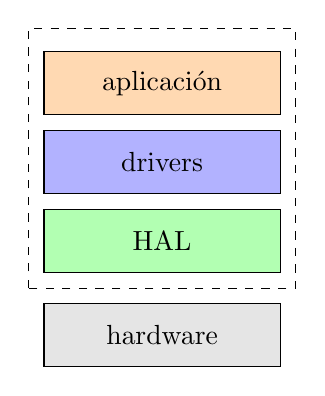
\begin{tikzpicture}
	% Define separated layers
	\node[draw, fill=orange!30, minimum width=3cm, minimum height=0.8cm] at (0, 2) {aplicación};
	\node[draw, fill=blue!30, minimum width=3cm, minimum height=0.8cm] at (0, 1.0) {drivers};
	\node[draw, fill=green!30, minimum width=3cm, minimum height=0.8cm] at (0, 0) {HAL};
	\node[draw, fill=gray!20, minimum width=3cm, minimum height=0.8cm] at (0, -1.2) {hardware};
	
	% Outline dashed box surrounding only the top three layers
	\draw[dashed] (-1.7, -0.6) rectangle (1.7, 2.7);
	\end{tikzpicture}
	\caption{Patrón de arquitectura de capas, obtenido a partir de presentaciones de clases de Ingeniería de Software \protect\footnotemark.}
	\label{fig:patroncapas}
\end{figure}
\footnotetext{Imagen obtenida de diapositiva de la materia Ingeniería de Software,  CESE, FIUBA, 2023.}

El patrón ``observar y reaccionar'', que se muestra en la figura \ref{fig:patronobservarreaccionar}, es la base del sistema de monitoreo. Su implementación en la capa de aplicación permitió la supervisión continua de los sensores y el procesamiento sistemático de los datos. El diseño implementó un mecanismo de notificación basado en el patrón de observador, donde los sensores funcionaron como sujetos observables, lo que generó eventos o cambios de estado. Por otro lado, los módulos de procesamiento y almacenamiento fueron diseñados como observadores, encargados de recibir y procesar las notificaciones emitidas por los sujetos observables.

\begin{figure}[H]
	\footnotesize
	\centering
	% Patron Obervar y reaccionar
	

\shorthandoff{>}
\begin{tikzpicture}[
node distance=0.5cm,
every node/.style={
	draw,
	rounded corners,
	minimum height=1cm,
	minimum width=2.5cm,
	align=center 
},
label/.style={    % Nuevo estilo para etiquetas
	draw=none,    % Sin borde
	minimum height=0cm,  % Sin altura mínima
	minimum width=0cm   % Sin ancho mínimo
}
]
% Definición de nodos
\node (observer) {proceso\\ observador};
\node[above=0.5cm of observer] (sensors) {sensores};
\node[right=2cm of observer] (analysis) {proceso de\\ análisis};
\node[right=2cm of analysis] (display) {proceso de\\ despliegue};
\node[above=0.5cm of display] (screen) {pantalla};
\node[below left=0.5cm and 0.5cm of analysis] (alarm) {proceso de\\ alarma};
\node[below right=0.5cm and 1cm of analysis] (reactor) {proceso reactor};
\node[below=of alarm] (alarmDevice) {alarma};
\node[below=of reactor] (otherDevice) {otro equipo};

% Conexiones
\draw[-latex] (sensors) -- (observer);
\draw[-latex] (observer) -- node[label, above] {valores de\\ sensor} (analysis);
\draw[-latex] (analysis) -- node[label, above] {valores a\\ desplegar} (display);
\draw[-latex] (display) -- (screen);
\draw[-latex] (analysis) -- (alarm);
\draw[-latex] (alarm) -- (alarmDevice);
\draw[-latex] (analysis) -- (reactor);
\draw[-latex] (reactor) -- (otherDevice);
\end{tikzpicture}
\shorthandon{>}
	\caption{Patrón arquitectónico: ``observar y reaccionar'' \protect\footnotemark.}
	\label{fig:patronobservarreaccionar}
\end{figure}
\footnotetext{Imagen obtenida de diapositiva de la materia Ingeniería de Software,  CESE, FIUBA, 2023.}

El tercer patrón implementado, ``segmentación de procesos'', estableció el flujo de datos entre los módulos del sistema. Un esquema de este patrón puede ser observado en la figura \ref{fig:patronsegmentacionprocesos}. Esta arquitectura definió etapas específicas para la adquisición, validación, procesamiento estadístico y almacenamiento de las mediciones. La segmentación aseguró la integridad de los datos mediante buffers intermedios entre etapas y mecanismos de verificación en cada transferencia. Esta implementación permitió el procesamiento secuencial de las mediciones y facilitó la detección de errores en el flujo de datos.

\begin{figure}[H]
	\centering
	\small
	% patron de segmentacion
		\shorthandoff{>}
		\begin{tikzpicture}[node distance=5cm, every node/.style={draw, rounded corners, minimum height=1.5cm, minimum width=2.2cm, align=center}]
			% Nodes
			\node (producer) {proceso\\ productor};
			\node[right of=producer] (buffer) {proceso\\ buffer};
			\node[right of=buffer] (consumer) {proceso\\ consumidor};
			\node[right=1cm of consumer, draw=none, minimum width=0.1cm] (ellipsis) {...};
			
			% Connections with labels outside of boxes
			\path[-latex] (producer) edge node[above, draw=none] {datos\\ producidos} (buffer);
			\path[-latex] (buffer) edge node[above, draw=none] {datos\\ consumidos} (consumer);
			\path[-latex] (consumer) edge (ellipsis);
		\end{tikzpicture}
		\shorthandon{>}
	\caption{ Patrón arquitectónico: “segmentación de procesos” \protect\footnotemark.}
	\label{fig:patronsegmentacionprocesos}
\end{figure}
\footnotetext{Imagen obtenida de diapositiva de la materia Ingeniería de Software,  CESE, FIUBA, 2023.}


\subsection{Integración de las estructuras y flujo de datos}

La figura \ref{fig:diagpatrones} presenta la integración de la arquitectura de software del sistema. La implementación estableció procesos interconectados para la gestión del flujo de datos, desde la adquisición en los sensores hasta el almacenamiento y transmisión de la información. Estos procesos incluyeron la validación de mediciones, el procesamiento estadístico, el almacenamiento local y la comunicación con sistemas remotos.

\begin{figure}[htpb]
	\centering
	\footnotesize
		
	\shorthandoff{<>} % Desactivar caracteres problemáticos
	
	
	\begin{tikzpicture}[ node distance=1cm]
	% Nodes
	%\draw[rounded corners] (0,0) rectangle (4,2);
	
	\node (observador) 
	[draw, rectangle, rounded corners, fill=blue!10!white, 
	align=center, yshift=2cm, xshift=0cm] 						
	{proceso\\ observador}; %\rotatebox{90}{\faMicrochip}};  
	
	\node (sensor1) 		
	[above left=of observador, draw, circle, fill=red!10!white, align=center, yshift=0.1cm, xshift=1cm] 	
	{\faSmog};
	
	\node (sensor2) 		
	[above=of observador, draw, circle, fill=red!10!white, align=center, yshift=-0.3cm, xshift=0.0cm] 	
	{ \faSmog};
	
	\node (sensor3)
	[above right=of observador, draw, circle, fill=red!10!white, align=center, yshift=0.1cm, xshift=-.80cm]
	{\faSmog};
	
	\node (rtc) 			
	[below =of observador, draw, circle, align=center,fill=red!10!white, yshift=0cm, xshift=0.0cm]  
	{\faClock[regular]};
	\node (sensorRTC) [below=of rtc,align=center, xshift=0 cm,yshift=1cm]     {\textbf{RTC} }; %\faCloudSunRain
	
	
	\node (tyh) 			
	[below  right=of observador, draw, circle, align=center,fill=red!10!white, yshift=0cm, xshift=-1.0cm]  {\faThermometerHalf};
	\node (sensorTyH) [below=of tyh, align=center, xshift=0.1 cm,yshift=1cm] 
	{\textbf{TyH} }; %\faCloudSunRain


	
	\node (sensores) [above =of sensor1,align=center, xshift=1 cm,yshift=-1cm]     {\textbf{sensores  \MPF} }; %\faCloudSunRain
	
	\node (aplicacion) 
	[right=2cm of sensores,align=center, xshift=-0.5 cm,yshift=0.2cm]     
	{\textbf{capa aplicación} }; %\faCloudSunRain
	
	\node (segmentacion) 		
	[right=of observador, draw, rectangle, rounded corners, fill=red!30!white, align=center, yshift=0cm, xshift=0cm] 						
	{ patrón \\ segmentación}	;
	
	\node (analisis) 		
	[right=of segmentacion, draw, rectangle, rounded corners, fill=blue!10!white, align=center, yshift=0cm, xshift=0cm] 						
	{proceso \\ de análisis};
	
	\node (despliegue) 		
	[right=of analisis, draw, rectangle, rounded corners, fill=blue!10!white, align=center, yshift=0cm, xshift=0cm] 						
	{proceso \\ despliegue};
	
	\node (alarma)
	[below left=of analisis, draw, rectangle, rounded corners, fill=blue!10!white, align=center, yshift=0cm, xshift=1cm] 						
	{proceso \\ alarma};
	
	\node (reactor) 		
	[below right=of analisis, draw, rectangle, rounded corners, fill=blue!10!white, 	align=center, yshift=0cm, xshift=0cm] 						
	{ proceso \\ reactor};
	
	\node (servidor) 		
	[below=0.4 cm of reactor,  align=center, yshift=0cm, xshift=0cm] 						
	{módulo\\inalámbrico \faWifi}; % https://www.ipgp.fr/~moguilny/LaTeX/fontawesome5Icons.pdf
	
	\node (led) 		
	[below=0.5cm of alarma,  align=center, yshift=0cm, xshift=0cm] 						
	{LED \faLightbulb};
	
	\node (memoria) 		
	[above=of despliegue,  align=center, yshift=0cm, xshift=0cm] 						
	{memoria \faSdCard };
	
	% Bounding Box
	\begin{scope}[on background layer]
	\node(aplicacion)[fill=orange!15,  draw, rectangle, rounded corners, fit=(aplicacion)(sensor1) (sensor2) (sensor3) (sensores) (despliegue) (rtc) (servidor) (alarma)] {};
	\node(driver)[below=of aplicacion,fill=blue!15,  draw, rectangle, rounded corners,
	minimum width=11cm, minimum height=0.8cm, , yshift=0.8cm, xshift=0cm]{capa drivers} ;
	\node(hal)[below=of driver,fill=green!10,  draw, rectangle, rounded corners,
	minimum width=11cm, minimum height=0.8cm, yshift=0.8cm]{capa HAL} ;
	\node(hardware)[below=of hal,fill=gray!10,  draw, rectangle, rounded corners,
	minimum width=11cm, minimum height=0.8cm,  yshift=0.5cm]{Hardware} ;
	\node[draw, dashed, fit=(aplicacion) (driver) (hal), inner sep=8pt, rounded corners] (box) {};
	\end{scope}
	
	% Arrows
	\draw[-] (observador) -- (sensor1);
	\draw[-] (observador) -- (sensor2);
	\draw[-] (observador) -- (sensor3);
	\draw[->] (observador) -- (segmentacion);
	\draw[->] (segmentacion) -- (analisis);
	\draw[->] (analisis) -- (despliegue);
	\draw[->] (despliegue) -- (memoria);
	\draw[->] (analisis) -- (reactor);
	\draw[->] (reactor) -- (servidor); % \faWifi
	\draw[->] (analisis) -- (alarma);
	\draw[->] (alarma) -- (led);
	\draw[-] (rtc) -- (observador);
	\draw[-] (tyh) -- (observador);
	
	\end{tikzpicture}
		\shorthandon{<>} 
	\caption{Arquitectura de bloques de los componentes del software.}
	\label{fig:diagpatrones}
\end{figure}


\subsection{Procesos principales}
Para el software se implementaron tres procesos fundamentales para la gestión de datos:

\subsubsection{Proceso observador}

Este proceso constituyó el punto de entrada del sistema, lo que permitió la adquisición de datos desde los sensores de temperatura, humedad, \MPF y el RTC. La implementación estableció un sistema de muestreo configurable con intervalos desde 10 minutos hasta 24 horas, lo que permitió adaptar el monitoreo a diferentes requisitos. Cada medición incorporó una marca temporal del RTC para asegurar la trazabilidad de los datos.

\subsubsection{Proceso de análisis}

El núcleo central del sistema recibió los datos del proceso observador mediante un buffer intermediario. Este módulo implementó las calibraciones, ejecutó cálculos estadísticos y validó la integridad de la información. El procesamiento incluyó el cálculo de promedios móviles, desviaciones estándar y la detección de valores atípicos para determinar la calidad del aire.

\subsubsection{Procesos de salida}

La arquitectura implementó tres componentes especializados:
\begin{itemize}
	\item Proceso de despliegue: gestionó el registro en memoria microSD, en datos con estructuras temporales de 10 minutos, 1 hora y 24 horas.
	\item Proceso reactor: manejó la transmisión de los datos hacia el módulo inalámbrico hacia un servidor remoto mediante protocolos estandarizados.
	\item Proceso de alarma: controló indicadores LED para proporcionar retroalimentación visual sobre el estado del sistema.
\end{itemize}

\subsection{Interfaces y comunicaciones}

El sistema implementó múltiples protocolos de comunicación para interactuar con sus componentes periféricos. La comunicación con los sensores \MPF se estableció mediante UART, mientras que la interfaz con el RTC utilizó el protocolo \IIC. El almacenamiento de los datos en la memoria microSD se realizó a través del protocolo SPI. La transmisión inalámbrica de datos empleó una interfaz UART adicional, y el control de señalización mediante LED se gestionó a través de GPIO.

La gestión de energía implementó un sistema de conmutación automática para mantener la operatividad ante fallos en el suministro eléctrico principal. El diseño incorporó un modo de bajo consumo que se activó cuando el sistema operó con batería de respaldo. Esto permitió reducir el consumo energético mediante la desactivación selectiva de periféricos no críticos, por ejemplo, el módulo de comunicación inalámbrica. Esta implementación incremento el tiempo de funcionamiento de las mediciones durante interrupciones eléctricas.


\section{Detalle de los componentes y responsabilidades}

La implementación del sistema estableció una arquitectura de procesos interconectados, donde cada componente ejecutó funciones específicas en el flujo de datos. Esta organización permitió la adquisición desde los sensores, el procesamiento de las mediciones y su posterior almacenamiento, tanto en la memoria local como en el servidor remoto.

Los procesos implementados se alinearon con los patrones arquitectónicos descritos, como se ilustra en las figuras \ref{fig:diagpatrones} y \ref{fig:diagsegmentacion}. La arquitectura integró seis componentes principales: el proceso observador para la adquisición de datos, el buffer intermediario para la gestión temporal, el proceso de análisis para la validación estadística, el proceso de despliegue para el almacenamiento local, el proceso reactor para la transmisión remota y el proceso de alarma para la señalización del estado del sistema.

\begin{figure}[htpb]
	\centering
	\footnotesize
		\shorthandoff{<>} % Desactivar caracteres problemáticos
	
	
	\begin{tikzpicture}[ node distance=2cm]
	% Nodes
	%\draw[rounded corners] (0,0) rectangle (4,2);
	
	\node (observador) 
	[draw, rectangle, rounded corners, fill=blue!10!white, 
	align=center, yshift=2cm, xshift=0cm] 						
	{proceso \\ observador}; %\rotatebox{90}{\faMicrochip}};  
	
	
	\node (buffer) 		
	[right=of observador,  draw, rectangle, rounded corners, fill=blue!10!white, align=center, yshift=0cm, xshift=1cm] 						
	{ proceso \\ buffer};
	
	\node (aplicacion) 
	[above =of observador,align=left, xshift=0.5 cm,yshift=-0.3cm]     
	{\textbf{capa aplicación} }; %\faCloudSunRain
	
	\node (segmentacion) 
	[above =of buffer,align=left, xshift=0 cm,yshift=-1.2cm]     
	{\textbf{patrón de segmentación} }; %\faCloudSunRain
	
	
	\node (analisis) 		
	[right=of buffer, draw, rectangle, rounded corners, fill=blue!10!white, align=center, yshift=0cm, xshift=1cm] 						
	{proceso \\ de análisis};
	
	% Nodos invisibles para las etiquetas de las flechas
	\node (etiqueta1) [left=of buffer, yshift=1.6cm, xshift=-0.2cm] {};
	\node (etiqueta2) [right=of buffer, yshift=1.6cm, xshift=0.2cm] {};
	
	
	
	
	% Arrows
	\draw[->] (observador) -- (buffer) 
	node[above, align=center, midway] 
	{datos \\ producidos};
	
	\draw[->] (buffer) -- (analisis) 
	node[above, align=center, midway] 
	{datos \\ consumidos};
	
	% Ajuste del cuadro segmentado para incluir las etiquetas
	\begin{scope}[on background layer]
	\node(aplicacion)
	[fill=orange!10,  draw, rectangle, inner sep=10pt, rounded corners, fit=(aplicacion) (observador) (analisis)(etiqueta2) ] {};
	\node[draw, dashed, fill=red!30!white, fit=(buffer) (etiqueta1) (etiqueta2), inner sep=4pt, rounded corners] (box) {};
	\end{scope}
	
	\end{tikzpicture}
		\shorthandon{<>} % Reactivar caracteres problemáticos
	\caption{Detalle con el patrón de segmentación del software.}
	\label{fig:diagsegmentacion}
\end{figure}



\subsection{Proceso observador:}

Este proceso se empleo durante la captura de datos,  los sensores de \MPF y el Reloj de Tiempo Real (RTC). Su tarea consistió en la recolección continua de información sobre la concentración de partículas en el aire, junto con marcas temporales para cada conjunto de datos. Posteriormente, estos datos son encaminados hacia la etapa de preprocesamiento (proceso buffer - segmentación de procesos).

Este proceso está encargado de solicitar y recabar datos de los sensores de \MPF en intervalos que pueden variar desde un minuto hasta horas, según la configuración establecida. Esta flexibilidad en la programación permite configurar la toma de muestras, adecuándose a diferentes necesidades de monitoreo y características específicas de cada sensor. Adicionalmente, el módulo se encargará de obtener del RTC y escribir en cada registro una marca temporal del dato. Una vez recolectados, estos datos son transmitidos al siguiente eslabón en el proceso, el \textit{``proceso buffer''}, para su posterior tratamiento.


\subsection{Proceso buffer:} 

El proceso buffer es un componente del patrón de segmentación, responsable del acondicionamiento y almacenamiento temporal de los datos. La implementación estableció una estructura intermedia entre el proceso observador y el proceso de análisis.

El diseño implementó tres niveles de almacenamiento temporal: un buffer de alta frecuencia con retención de 10 minutos para datos instantáneos; un buffer horario para el cálculo de promedios móviles; y un buffer diario para la generación de estadísticas de 24 horas. Este proceso recibió los datos del proceso observador, ejecutó la validación preliminar y el formateo de la información, para su posterior transferencia al proceso de análisis. La tabla \ref{tab:buffer_estructura} presenta la organización de los datos en cada nivel de almacenamiento.

\begin{table}[htbp]
	\centering
	\small
	\caption{Ejemplo de estructura de datos.}
	\label{tab:buffer_estructura}
	% ejemplos estructura de datos
\begin{tabular}{lcc}
	\toprule
	\textbf{Atributo} & \textbf{Tipo de dato} & \textbf{Formato} \\
	\midrule
	idsensor    & int   & - \\
	fecha-hora  & int   & AAMMDDHHMM \\
	frecuencia  & int   & - \\
	\MPF        & float & - \\
	temperatura & int   & - \\
	humedad     & int   & - \\
	\bottomrule
\end{tabular}
\end{table}                           


\subsection{Proceso de análisis}
El proceso de análisis implementó el cálculo numérico y la validación estadística de los datos provenientes del buffer. Las operaciones incluyeron la corrección de las concentraciones mediante parámetros de calibración y el cálculo de estadísticos para diferentes intervalos temporales (10 minutos, 1 hora y 24 horas).

Se aplicaron métodos numéricos que permitió estimar la calidad de las mediciones mediante el cálculo de valores centrales y de dispersión. Esta incorporó algoritmos para la detección de valores atípicos y la evaluación de la concordancia entre los tres sensores de \MPF. Este procesamiento generó índices de confiabilidad para cada medición y activó alarmas ante la detección de anomalías en el funcionamiento de los sensores.

\subsection{Proceso de despliegue}
El proceso de despliegue implementó la gestión del almacenamiento de datos en la memoria microSD. Este módulo recibió la información procesada del proceso de análisis y ejecutó las operaciones de escritura en el sistema de archivos.

La implementación estableció una estructura jerárquica de almacenamiento con tres niveles temporales: registros de 10 minutos, promedios horarios y resúmenes diarios. El sistema generó archivos independientes para cada período. Incorpora metadatos que identificaron el origen y características de las mediciones. Esta organización permitió la trazabilidad de los datos y facilitó su posterior procesamiento.

\subsection{Proceso reactor}

El proceso reactor implementó la comunicación de datos entre el sistema y un servidor remoto mediante el módulo Wi-Fi. Este componente estableció la interfaz entre el proceso de análisis y la transmisión inalámbrica de información.

Se incorporarón tres funciones principales: la gestión de la configuración de red inalámbrica, el establecimiento del protocolo de transferencia de archivos (FTP), y la transmisión de datos procesados. El sistema transmitió los registros temporales organizados en intervalos de 10 minutos, promedios horarios y resúmenes diarios. Cada paquete de datos incluyó metadatos de identificación que especificaron el origen y características de las mediciones transmitidas.

\subsection{Proceso de alarma}
El proceso de alarma implementó la señalización visual del estado operativo del sistema mediante un indicador LED. Este módulo procesó los códigos de estado generados por los distintos componentes y tradujo esta información en patrones específicos de señalización luminosa.

Se estableció una codificación basada en frecuencias de parpadeo del LED para indicar diferentes estados operativos: funcionamiento normal, fallos en sensores, errores de comunicación y estados del sistema. Esta interfaz visual proporcionó retroalimentación inmediata sobre el estado del instrumento al usuario.

\subsection{Módulo de energía}
El módulo de energía implementó la gestión y distribución de alimentación eléctrica para todos los componentes del sistema. La arquitectura estableció un sistema de conmutación automática entre la fuente principal de \SI{220}{\volt} y una batería de respaldo.

La incorporó dos modos de operación: normal y bajo consumo. El modo normal operó con la fuente principal, mientras que el modo de bajo consumo se activó de manera automática ante interrupciones en el suministro eléctrico. Este último redujo el consumo mediante la desactivación selectiva de componentes no críticos, lo que permitió mantener las funciones esenciales del sistema durante períodos limitados de operación con batería.

\section{Responsabilidades de las interfaces periféricas}

Descripción de las principales funcionalidades con los componentes y sensores periféricos.

\subsection{Sensores \MPF}
La interfaz con los sensores de \MPF constituyó el componente principal para la adquisición de datos de concentración de material particulado. Se estableció la comunicación mediante el protocolo UART, seleccionado por sus características de transmisión serie asíncrona y compatibilidad con los sensores SPS30.

El proceso observador gestionó la operación de los sensores mediante una secuencia definida de comandos: inicialización, configuración de parámetros de medición, adquisición de datos y verificación de estado. Este protocolo de comunicación permitió la obtención sistemática de mediciones de concentración de \MPF con una resolución temporal programable.

\subsection{Reloj de tiempo real RTC}

Con los datos entregados por el RTC DS3231 se implementó la base de tiempo del sistema, necesario para el registro temporal de las mediciones. El proceso observador gestionó la comunicación con este dispositivo mediante el protocolo \IIC, seleccionado por su compatibilidad y eficiencia en la transmisión de datos temporales.

Se incorporaron dos funciones principales: la sincronización periódica del sistema y el etiquetado temporal de las mediciones de \MPF. Esta interfaz proporcionó marcas de tiempo con precisión de \SI{\pm2}{\ppm}.

\subsection{Almacenamiento microSD}

Se integró un módulo de almacenamiento con memoria microSD para el registro local de datos. El proceso de despliegue gestionó las operaciones de escritura y lectura mediante el protocolo SPI, que operó a una frecuencia de \SI{42}{\mega\hertz}.

Se incorporó el sistema de archivos FAT32 y estableció un buffer de escritura de \SI{512}{\byte} para optimizar las operaciones de almacenamiento. Esta interfaz permitió el registro estructurado de las mediciones.
	
\subsection{Módulo de conexión inalámbrica}

El software integró la comunicación con un servidor remoto mediante el módulo Wi-Fi ESP8266. El proceso reactor estableció la interfaz entre el sistema de medición y la transmisión de datos.

Se incorporó tres funciones principales: la configuración de la conexión Wi-Fi, la gestión del protocolo FTP para la transferencia de archivos, y la comunicación UART con el módulo ESP8266 a \SI{115200}{\baud}. Esta arquitectura permitió la transmisión automática de los datos almacenados hacia el servidor remoto mediante una conexión TCP/IP.
	
	
\subsection{Señal de estado LED}

Se incorporó un indicador visual mediante LED para la señalización del estado operativo. El proceso de alarma gestionó la codificación de estados del sistema mediante patrones de parpadeo predefinidos.

Se utilizó un puerto GPIO configurado en modo PWM para el control del LED. Esta interfaz estableció diferentes frecuencias de parpadeo para señalizar distintas condiciones operativas: funcionamiento normal; errores en sensores; fallos de comunicación; y estados de la alimentación. Este método proporcionó retroalimentación inmediata sobre el estado del sistema al usuario.
	
	
\subsection{Gestión de energía}
El módulo de gestión de energía implementó un sistema de monitorización del suministro eléctrico mediante un puerto GPIO configurado en modo lectura. Este componente supervisó el estado de la alimentación principal y controló la conmutación automática hacia la batería de respaldo.

Se definieron dos funciones principales: la detección de interrupciones en el suministro de \SI{220}{\volt} y la activación del modo de bajo consumo. El sistema utilizó el estado binario del GPIO para determinar la fuente de alimentación activa y ejecutar la transición entre modos de operación, lo que aseguró la continuidad del monitoreo ante fallos en el suministro eléctrico.
	
	

\section{Implementación de protocolos}

La integración de protocolos de comunicación en el sistema de medición de \MPF estableció las interfaces entre módulos y periféricos. Se incorporaron protocolos estandarizados para asegurar la confiabilidad y eficiencia en la transferencia de datos.

\subsection{Protocolo UART para sensores de \MPF}
La comunicación con los sensores SPS30 se implementó mediante una interfaz UART en configuración maestro-esclavo. El protocolo estableció los siguientes parámetros operativos:

\begin{itemize}
	\item Velocidad de comunicación: \SI{100}{\kilo\hertz}.
	\item Direccionamiento: asignación de dirección única por sensor (0x69).
	\item Buffer de recepción: \SI{32}{\byte} para datos de concentración.
	\item Tiempo máximo de transacción: \SI{30}{\milli\second}.
\end{itemize}

La secuencia de comunicación sigue el  patrón de la figura \ref{fig:i2c_sequence}.

\begin{figure}[h]
	\centering
	\small
	% secuencia de comunicacion SPS30 
	\shorthandoff{>}
	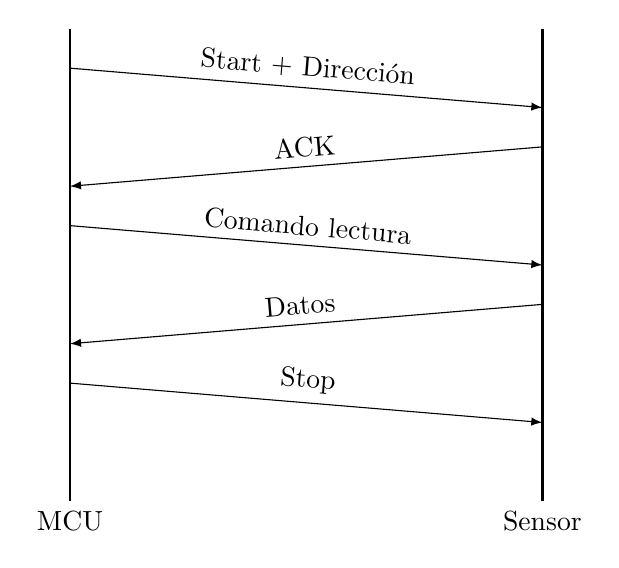
\begin{tikzpicture}[
	node distance=2cm,
	every node/.style={align=center},
	label/.style={draw=none}
	]
	% Líneas de tiempo verticales
	\draw[thick] (0,0) -- (0,-6) node[below] {MCU};
	\draw[thick] (6,0) -- (6,-6) node[below] {Sensor};
	
	% Mensajes
	\draw[-latex] (0,-0.5) -- (6,-1) node[midway, above, sloped] {Start + Dirección};
	\draw[-latex] (6,-1.5) -- (0,-2) node[midway, above, sloped] {ACK};
	\draw[-latex] (0,-2.5) -- (6,-3) node[midway, above, sloped] {Comando lectura};
	\draw[-latex] (6,-3.5) -- (0,-4) node[midway, above, sloped] {Datos \MPF};
	\draw[-latex] (0,-4.5) -- (6,-5) node[midway, above, sloped] {Stop};
	\end{tikzpicture}
	\shorthandon{>}
	\caption{Secuencia de comunicación UART con sensor SPS30.}
	\label{fig:i2c_sequence}
\end{figure}

\subsection{Protocolo SPI para almacenamiento}
Se aplicó el protocolo SPI de comunicación con la memoria microSD. El diseño incorporó las siguientes especificaciones técnicas:

\begin{itemize}
	\item Frecuencia de operación: \SI{42}{\mega\hertz} en modo maestro.
	\item Sistema de archivos: FAT32 con sectores de \SI{512}{\byte}.
	\item Transferencia de datos: DMA para optimización de recursos.
	\item Buffer circular: \SI{512}{\byte} para gestión de escritura.
\end{itemize}

\subsection{UART para comunicación inalámbrica}
La implementación de la comunicación con el módulo ESP8266 estableció una interfaz UART con los siguientes parámetros operativos:
\begin{itemize}
	\item Velocidad de transmisión: \SI{115200}{\baud}.
	\item Control de flujo: señales hardware RTS/CTS.
	\item Buffer de transmisión: \SI{256}{\byte}.
	\item Tiempo de espera máximo: \SI{100}{\milli\second}.
\end{itemize}
La capa de aplicación implementó los siguientes mecanismos de control:
\begin{itemize}
	\item Establecimiento de conexión mediante handshaking.
	\item Sistema de retransmisión automática ante fallos.
	\item Verificación de integridad mediante CRC-16.
	\item Estructura de trama con campos de cabecera y cola.
\end{itemize}

\subsection{GPIO para control y monitoreo}
Se estableció tres funciones principales para la puesta en funcionamiento de las interfaces GPIO :
\begin{itemize}
	\item Señalización visual: control del LED mediante modulación PWM.
	\item Supervisión energética: detección del estado de alimentación.
	\item Control de energía: gestión del modo de bajo consumo.
\end{itemize}
\subsection{Gestión de errores y recuperación}
El sistema implementó mecanismos de protección y recuperación ante fallos de comunicación:
\begin{itemize}
	\item Sistema de temporización: límites de tiempo para cada transacción.
	\item Recuperación automática: reinicialización de periféricos ante errores.
	\item Sistema de respaldo: buffer temporal para datos críticos.
	\item Trazabilidad: registro de eventos de error en memoria no volátil.
\end{itemize}

\subsection{Optimización del rendimiento}
Al instrumento se le incorporó mecanismos específicos para optimizar la eficiencia del sistema:
\begin{itemize}
	\item Transferencia de datos: DMA para operaciones críticas.
	\item Gestión de eventos: sistema de interrupciones para respuesta inmediata.
	\item Administración de memoria: buffers circulares para gestión eficiente.
	\item Planificación: esquema de prioridades para tareas de comunicación.
\end{itemize}

El diseño modular permitió el mantenimiento y actualización independiente de cada protocolo, mientras que los mecanismos de optimización aseguraron un uso eficiente de los recursos del microcontrolador.

	
\section{Ajuste y calibración de sensores y transmisores}
Se estableció un proceso sistemático de calibración y ajuste del sistema de medición de \MPF para asegurar la precisión y trazabilidad de las mediciones. Este procedimiento consideró las características específicas de los sensores SPS30 y las condiciones ambientales de operación.
\subsection{Calibración de sensores \MPF}
El protocolo de calibración se implementó en dos etapas principales:
\begin{enumerate}
	\item Calibración de fábrica: Los sensores incorporaron una calibración inicial contra instrumentos de referencia:
	\begin{itemize}
		\item Fotómetro TSI DustTrak™ DRX 8533: validación gravimétrica.
		\item Espectrómetro óptico TSI OPS 3330: caracterización de distribución de partículas.
	\end{itemize}
	\item Calibración en campo: La implementación requirió ajustes específicos según condiciones locales:

	\begin{itemize}
		\item Correlación con monitor Beta de referencia.
		\item Factor de corrección por humedad relativa.
		\item Compensación por temperatura ambiente.
	\end{itemize}
\end{enumerate}


\subsection{Modelo de corrección}
Se incorporó un modelo de corrección lineal para el ajuste de las mediciones:
\begin{equation}
C_{corregida} = a \cdot C_{medida} + b \cdot H + c \cdot T + d
\end{equation}
Donde las variables representan:
\begin{itemize}
	\item $C_{corregida}$: concentración ajustada (\si{\micro\gram\per\cubic\meter}).
	\item $C_{medida}$: concentración del sensor SPS30.
	\item $H$: humedad relativa (\%).
	\item $T$: temperatura (\si{\celsius}).
	\item $a$, $b$, $c$, $d$: coeficientes determinados  de manera experimental.
\end{itemize}

\subsection{Procedimiento de calibración}
El procedimiento de calibración en campo estableció cinco etapas secuenciales:
\begin{enumerate}
	\item Acondicionamiento inicial: período de estabilización de 24 horas.
	\item Adquisición de datos: mediciones simultáneas con monitor Beta de referencia.
	\item Procesamiento estadístico: determinación de coeficientes mediante regresión lineal.
	\item Verificación: validación con conjunto de datos independiente.
	\item Programación: actualización del firmware con factores de corrección.
\end{enumerate}


\subsection{Validación y control de calidad}
Se ejecutaron mecanismos automáticos para el aseguramiento de la calidad de las mediciones:
\begin{itemize}
	\item Sistema de detección de valores atípicos.
	\item Validación cruzada entre los tres sensores redundantes.
	\item Monitoreo continuo de variables ambientales.
	\item Sistema de notificación para recalibración programada.
\end{itemize}
\subsection{Mantenimiento y recalibración}
El protocolo de mantenimiento estableció un cronograma sistemático de verificación:
\begin{itemize}
	\item Validación trimestral con monitor Beta de referencia.
	\item Ciclo automático de limpieza cada \SI{168}{\hour}.
	\item Recalibración integral anual.
	\item Compensación de la deriva temporal mediante ajuste de coeficientes.
\end{itemize}

Esta implementación sistemática de calibración y control busca asegurar la estabilidad y precisión de las mediciones a largo plazo. La arquitectura con tres sensores permitió la validación continua de datos y la detección temprana de desviaciones en el sistema de medición.

%\section{Análisis del software}
% 
%La idea de esta sección es resaltar los problemas encontrados, los criterios utilizados y la justificación de las decisiones que se hayan tomado.
%
%Se puede agregar código o pseudocódigo dentro de un entorno lstlisting con el siguiente código:
%
%\begin{verbatim}
%\begin{lstlisting}[caption= "un epígrafe descriptivo"]
%	las líneas de código irían aquí...
%\end{lstlisting}
%\end{verbatim}
%
%A modo de ejemplo:
%
%\begin{lstlisting}[label=cod:vControl,caption=Pseudocódigo del lazo principal de control.]  % Start your code-block
%
%#define MAX_SENSOR_NUMBER 3
%#define MAX_ALARM_NUMBER  6
%#define MAX_ACTUATOR_NUMBER 6
%
%uint32_t sensorValue[MAX_SENSOR_NUMBER];		
%FunctionalState alarmControl[MAX_ALARM_NUMBER];	//ENABLE or DISABLE
%state_t alarmState[MAX_ALARM_NUMBER];						//ON or OFF
%state_t actuatorState[MAX_ACTUATOR_NUMBER];			//ON or OFF
%
%void vControl() {
%
%	initGlobalVariables();
%	
%	period = 500 ms;
%		
%	while(1) {
%
%		ticks = xTaskGetTickCount();
%		
%		updateSensors();
%		
%		updateAlarms();
%		
%		controlActuators();
%		
%		vTaskDelayUntil(&ticks, period);
%	}
%}
%\end{lstlisting}




%	%!TEX root = ../T1_Gomez_Luis_.tex

\chapter{Ensayos y resultados} % Main chapter title
\label{Chapter4} % For referencing this chapter elsewhere, use \ref{Chapter4}

%----------------------------------------------------------------------------------------
%	SECTION 1
%----------------------------------------------------------------------------------------

Este capítulo presenta la evaluación del sistema de medición de \MPF desarrollado, abarcando validación técnica, caracterización metrológica y rendimiento operativo. Se analizaron los resultados de las pruebas realizadas sobre el diseño electrónico, el sistema de alimentación y la implementación del software mediante un banco de pruebas estructurado. Se evalúa la calidad metrológica del instrumento a través del análisis de correlación entre los tres sensores redundantes y su comparación con equipos de referencia. La caracterización operativa incluye la verificación de la completitud de datos adquiridos, el análisis de patrones temporales de concentración, y la respuesta del instrumento ante un evento controlado de alta contaminación. Los resultados obtenidos, presentados mediante análisis estadístico y visualizaciones temporales, muestran que el sistema alcanza los niveles de confiabilidad y precisión requeridos para aplicaciones de monitoreo ambiental urbano.

\section{Banco de prueba} 


%	1	Descripción de las herramientas utilizadas para probar el dispositivo	Imágenes de equipos de prueba	Métodos de prueba y sus parámetros


El banco de pruebas se estructuró en cuatro categorías funcionales complementarias: instrumentación electrónica, validación metrológica, verificación de hardware y pruebas de software.

La instrumentación electrónica comprendió equipos para la caracterización y diagnóstico de los circuitos. Se utilizó un analizador lógico de \SI{24}{\mega\hertz} con 8 canales para la verificación de protocolos de comunicación (\IIC, SPI, UART), lo que permitió monitorizar en tiempo real las transacciones de datos entre el microcontrolador y los periféricos. Para el análisis de señales de alta frecuencia, se empleó un osciloscopio FNIRSI1014D de \SI{100}{\mega\hertz}, que facilitó la medición de tiempos de respuesta, detección de interferencias y verificación de integridad de señales críticas. Las mediciones de parámetros eléctricos se realizaron con un multímetro digital TMT460012, con resolución de \SI{0.01}{\milli\volt} para tensión y \SI{0.1}{\micro\ampere} para corriente. La alimentación controlada del sistema durante las pruebas se implementó mediante una fuente regulada Jesverty SPS-3005 con rango de \SIrange{0}{30}{\volt} y capacidad de corriente de \SI{5}{\ampere}.

Para la validación metrológica, las mediciones de \MPF se contrastaron con un instrumento de referencia Grimm y equipo certificado por su alta precisión (\SI{\pm2}{\percent}) en el análisis óptico de partículas atmosféricas dentro del rango de \SIrange{0.3}{10}{\micro\meter}. Esta comparación se realizó en dos escenarios: bajo condiciones controladas de laboratorio y en ambiente real, lo que expone a los sensores a las condiciones atmosféricas urbanas durante un período de 72 horas. Este enfoque dual permitió determinar tanto la exactitud y precisión del instrumento como su comportamiento en condiciones operativas reales.

La verificación del hardware se efectuó mediante un proceso sistemático que incluyó la comprobación del cumplimiento de las reglas de diseño de circuito impreso utilizó las herramientas integradas en KiCad. Este proceso verificó parámetros críticos como anchos de pista, distancias mínimas entre elementos y diámetros de vías. Adicionalmente, componentes  como inductores, capacitores y resistencias se caracterizaron individualmente con un medidor LCR-P1 de FNIRSI, que proporcionó datos  sobre sus propiedades eléctricas y tolerancias reales, lo que permite validar que sus valores se encontraban dentro de los márgenes establecidos para garantizar el funcionamiento correcto del circuito.

Las pruebas de software implementaron metodologías de validación mediante el framework Ceedling, que permitió la automatización de pruebas unitarias en lenguaje C. Esta aproximación posibilitó la evaluación independiente de cada módulo del firmware, facilitó la detección temprana de errores lógicos o de implementación. La integración de las herramientas Unity y CMock dentro del framework proporcionó capacidades para la creación de objetos simulados (\textit{mocks}) y aserciones específicas para validar el comportamiento esperado de las funciones. La verificación de comunicaciones se complementó con un terminal UART Cutecom, configurado a \SI{115200}{\baud}, para la inspección detallada de los datos transmitidos entre el sistema y los dispositivos periféricos, lo que facilitó la verificación del cumplimiento de los protocolos establecidos.

Las tablas \ref{tab:pruebas} y  \ref{tab:pruebas2} presentan un resumen  de los instrumentos empleados en el banco de pruebas. Esta detalla las características técnicas y función específica en el proceso de validación.





%\section{Pruebas funcionales del hardware}
%\label{sec:pruebasHW}

%La idea de esta sección es explicar cómo se hicieron los ensayos, qué resultados se obtuvieron y analizarlos.




\section{Evaluación del software}
%	3	Evaluación del rendimiento del hardware y herramientas empleadas para su evaluación	Fotos del prototipo final	Tabla con herramientas empleadas


La validación del sistema de medición de \MPF se enfocó en garantizar la precisión y confiabilidad del subsistema de análisis, identificado como componente crítico con una importancia relativa del 24\% según los criterios de diseño establecidos. Este componente procesa los datos provenientes de los sensores ópticos y realiza los cálculos estadísticos necesarios para determinar las concentraciones del contaminante.

\subsection{Metodología de pruebas de software}

Se implementó el \textit{Método del Árbol de Clasificación} (CTM) como estrategia principal para el diseño y ejecución de los casos de prueba. Esta técnica permitió una cobertura  y sistemática de los posibles escenarios de operación, lo que facilita la identificación de errores potenciales en el tratamiento de datos. El proceso consistió en cuatro etapas secuenciales:

\begin{enumerate}
	\item Definición de clases de equivalencia: se estableció categorías para los tipos de datos de entrada, lo que incluyó concentraciones dentro de los límites operativos (\SIrange{0.5}{500}{\micro\gram\per\cubic\meter}), valores por debajo del límite mínimo de cuantificación, mediciones que exceden el límite máximo de linealidad y casos atípicos como valores negativos o nulos.
	
	\item Construcción del árbol de clasificación: se desarrolló una estructura jerárquica que representa las diferentes clases de equivalencia y las relaciones entre ellas, lo que permitió la identificación de combinaciones específicas de condiciones para cada caso de prueba.
	
	\item Derivación de casos de prueba: a partir del árbol de clasificación, se identificó cinco escenarios representativos que abarcan las principales condiciones de operación y casos límite del sistema.
	
	\item Ejecución y análisis de resultados: se utilizó el framework Ceedling, junto con las herramientas Unity y CMock, para implementar y automatizar la ejecución de las pruebas unitarias.
\end{enumerate}

\subsection{Casos de prueba implementados}

Se desarrollaron cinco casos  para evaluar la función \texttt{calculateAverage} de la API \texttt{ParticulateDataAnalyzer}, responsable del cálculo del promedio de concentraciones de MP$_{2,5}$ bajo diferentes condiciones:

\begin{table}[h]
	\centering
	\small
	\caption{Resumen de los casos de prueba aplicados al subsistema de análisis.}
	\label{tab:casos-prueba-software}
	\begin{tabular}{c p{4.5cm} p{4.5cm} c }
		\hline
		\textbf{Test} & \textbf{Escenario} & \textbf{Objetivo} & \textbf{Resultado} \\
		\hline
		1 & Valores dentro del rango con algunos por debajo del límite de cuantificación & Verificar exclusión correcta de valores $< \SI{0.5}{\micro\gram\per\cubic\meter}$ & \SI{302.5}{\micro\gram\per\cubic\meter} \\
		
		2 & Datos válidos con algunos valores por encima del máximo y negativos & Comprobar manejo adecuado de valores fuera de rango superior y negativos & \SI{286.07}{\micro\gram\per\cubic\meter} \\
		
		3 & Arreglo completo de datos nulos & Validar respuesta ante ausencia total de datos válidos & $-999$ \\
		
		4 & Todos los valores dentro del rango permitido & Confirmar cálculo correcto con datos completamente válidos & \SI{316.67}{\micro\gram\per\cubic\meter} \\
		
		5 & Arreglo sin datos válidos (todos bajo límite) & Verificar comportamiento con datos insuficientes para cálculo & $-999$ \\
		\hline
	\end{tabular}
\end{table}

El caso de prueba 1 evaluó el procesamiento de un conjunto de datos donde la mayoría se encontraba dentro del rango operativo, lo que incluyó valores ligeramente por debajo del límite inferior de cuantificación (\SI{0.4}{\micro\gram\per\cubic\meter} y \SI{0.3}{\micro\gram\per\cubic\meter}). Esta prueba verificó que el sistema excluyera correctamente estos valores del cálculo del promedio y utilizara solo los 16 valores válidos restantes.

El caso 2 analizó el manejo de valores extremos, lo que incorporó tanto concentraciones negativas (\SI{-480}{\micro\gram\per\cubic\meter}) como mediciones superiores al límite máximo de linealidad (\SI{590}{\micro\gram\per\cubic\meter} y \SI{895}{\micro\gram\per\cubic\meter}). Esta prueba fue particularmente significativa para validar la robustez del sistema ante lecturas anómalas o errores de medición.

Los casos 3 y 5 evaluaron situaciones límite donde no existían datos válidos para el cálculo, ya sea por un arreglo completamente vacío o con datos por debajo del umbral mínimo de cuantificación. Ambos casos verificaron que el sistema respondiera adecuadamente con un valor de error predefinido ($-999$), lo que señaló la imposibilidad de realizar el cálculo.

El caso 4 representó un escenario ideal con todos los valores dentro del rango operativo permitido, lo que verificó la precisión del cálculo bajo condiciones óptimas de funcionamiento.

\subsection{Implementación de las pruebas}

Las pruebas se codificaron con el framework Ceedling, que integra las herramientas Unity y CMock para la automatización de pruebas unitarias en lenguaje C (ver figura \ref{fig:resultados-pruebas}). Cada caso de prueba se implementó como una función independiente que preparaba los datos de entrada, ejecutaba la función bajo evaluación y verificaba que el resultado correspondiera al valor esperado mediante aserciones.

La función \texttt{calculateAverage} evaluada realiza el procesamiento de un arreglo de valores flotantes que representan concentraciones de \MPF, con los siguientes pasos:

\begin{enumerate}
	\item Verifica si el arreglo está vacío mediante la función \texttt{isArrayEmpty}.
	\item Inicializa variables para sumatoria y conteo de valores no válidos.
	\item Recorre cada elemento del arreglo, lo que validó cada valor mediante la función \texttt{maskIsDataTrue}.
	\item Para los valores válidos, acumula la suma; para los inválidos, incrementa el contador.
	\item Recalcula el número efectivo de datos válidos.
	\item Verifica que exista al menos un valor válido antes de realizar la división.
	\item Retorna el promedio calculado o un valor de error predefinido.
\end{enumerate}

\begin{figure}[h]
	\centering
	\includegraphics[width=0.7\linewidth]{Figures/captura_ceedling}
	\caption{Resultados de la ejecución de las pruebas unitarias mediante Ceedling.}
	\label{fig:resultados-pruebas}
\end{figure}

\subsection{Resultados y mejoras implementadas}

La ejecución de los casos de prueba permitió identificar un error en la implementación de la función \texttt{calculateAverage}, específicamente en la validación de valores por encima del límite máximo de linealidad. Este hallazgo permitió la corrección temprana de un problema que podría haber afectado el cálculo de los promedios de \MPF durante la operación del instrumento.

Tras la detección del error, se implementaron las siguientes mejoras:

\begin{itemize}
	\item Modificación de la función \texttt{maskIsDataTrue} para incorporar explícitamente la validación del límite superior de \SI{500}{\micro\gram\per\cubic\meter}.
	\item Refinamiento de la documentación del código para especificar claramente los rangos de valores aceptables.
	\item Incorporación de mensajes de error más descriptivos para facilitar la identificación de problemas en tiempo de ejecución.
	\item Optimización del algoritmo para mejorar el rendimiento en el procesamiento de grandes volúmenes de datos.
\end{itemize}

Los criterios de aceptación establecidos definieron una precisión con desviación estándar no superior al 5\% para el cálculo del promedio, requisito que fue verificado y cumplido mediante los casos de prueba implementados. Adicionalmente, se estableció un umbral mínimo del 75\% de datos válidos para considerar representativo un promedio horario, criterio que fue incorporado en la lógica de procesamiento y verificado mediante los casos de prueba.

La aplicación del MAT proporcionó un marco sistemático para diseñar, documentar y comunicar los casos de prueba. Esto aseguro la trazabilidad de los requisitos funcionales hasta su verificación final.	


\section{Pruebas de hardware}

Esta sección presenta los resultados de la evaluación de los componentes físicos del sistema de medición de \MPF. Se analizaron los resultados de la verificación del diseño electrónico, la caracterización individual de componentes críticos y las pruebas del sistema de alimentación. 

\subsection{Resultados del diseño electrónico}

La verificación del diseño electrónico  evaluó el cumplimiento de las reglas de diseño especificadas en las tablas \ref{tab:reglas_pcb} y \ref{tab:clases_redes} del Apéndice \ref{AppendixB}. Esta metodología integró herramientas de validación automática disponibles en KiCad 6.0 con inspección visual detallada, lo que permitió identificar y corregir discrepancias en parámetros críticos como anchos de pista (mínimo \SI{0.25}{\milli\meter} para señales, \SI{0.5}{\milli\meter} para potencia), distancias mínimas entre elementos (\SI{0.2}{\milli\meter}) y diámetros de vías (\SI{0.4}{\milli\meter} para señal, \SI{0.8}{\milli\meter} para potencia).

El diseño cumplió con las especificaciones técnicas establecidas en aproximadamente 90\% de la superficie de la PCB, a excepción de áreas específicas correspondientes al conector de memoria microSD y los circuitos integrados DS3231 y 74LVC125U8 (ver figura \ref{fig:pcbdetalle}). Para estos componentes de encapsulado predefinido fue necesario implementar zonas de exclusión de reglas de diseño, lo que redujo localmente la separación mínima a \SI{0.15}{\milli\meter} debido a las restricciones impuestas por su geometría de pines. Esta modificación  no comprometió la funcionalidad ni la fiabilidad del circuito. 

\begin{figure} [!hbp]
	\centering
	\includegraphics[width=0.7\linewidth]{Figures/PCB_detalle}
	\caption{Detalle de una sección  de la PCB donde se observan los anchos de pistas diferenciados para señal (\SI{0.25}{\milli\meter}) y potencia (\SI{0.5}{\milli\meter}), márgenes mínimos de separación y zonas de exclusión implementadas para los componentes de encapsulado predefinido.}
	\label{fig:pcbdetalle}
\end{figure}

El diseño incorporó además soluciones específicas para optimizar la manufactura y la integridad de señal, tales como alivios térmicos para pads de alta corriente, planos de tierra en capas internas para reducción de EMI, y pistas de impedancia controlada  para las líneas de comunicación críticas SPI y UART. Estas características de diseño, apreciables en la figura \ref{fig:detallepcb3d}, contribuyeron  a la robustez del sistema en términos de estabilidad eléctrica y resistencia a interferencias electromagnéticas externas, aspectos fundamentales para la precisión de las mediciones de \MPF.

\begin{figure} [!hbp]
	\centering
	\includegraphics[width=0.7\linewidth]{Figures/Detalle_PCB_3D}
	\caption{Visualización de la PCB donde se aprecian los planos de tierra para reducción de interferencias (\SI{60}{\percent} de cobertura en capa superior), alivios térmicos para componentes de potencia, y vías  para estabilización de impedancia.}
	\label{fig:detallepcb3d}
\end{figure}


\newpage
\subsection{Verificación de componentes}

Previo a la integración del sistema completo, se realizó una etapa de verificación individualizada de cada componente crítico. Esta fase permitió detectar tempranamente posibles defectos y garantizar que todos los elementos cumplieran con las especificaciones técnicas requeridas. Se caracterizaron los componentes pasivos (resistencias, capacitores e inductores) mediante el medidor LCR-P1 de FNIRSI, lo que permite verificar sus valores nominales y tolerancias. Los sensores SPS30 fueron sometidos a pruebas funcionales en ambiente controlado para validar sus respuestas ópticas y calibración inicial. El microcontrolador STM32F429 y el módulo ESP8266 fueron verificados mediante pruebas de comunicación y respuesta a comandos específicos. Este proceso permitió asegurar la calidad individual de cada componente antes de su inclusión en el sistema integrado. Esta condición minimiza el riesgo de fallas durante la operación del instrumento.

\subsubsection{Resultados de la caracterización del sistema de alimentación}

Esta sección presenta los resultados obtenidos durante la evaluación del sistema de alimentación implementado para el instrumento de medición de \MPF. La caracterización se centró en los parámetros críticos para asegurar la precisión de las mediciones: estabilidad de tensión, nivel de ruido eléctrico y respuesta ante conmutaciones de fuente.

\subsubsection{Evaluación de componentes de ruido}

Los resultados de las pruebas iniciales con fuentes de alimentación convencionales mostraron niveles significativos de interferencia eléctrica, como se presenta en la figura \ref{fig:fuente_sin_filtro}. El análisis de estos datos reveló componentes de ruido con amplitudes de hasta \SI{78}{\milli\volt} pico-pico en frecuencias entre \SIrange{100}{150}{\kilo\hertz}.

\begin{figure}[h]
	\centering
	\includegraphics[width=0.8\linewidth]{Figures/test_fuente_condiciones_iniciales.JPEG}
	\caption{Registro de componentes de ruido en la fuente convencional con transitorios de alta frecuencia (\SI{138}{\kilo\hertz}) y amplitudes de aproximadamente \SI{78}{\milli\volt} pico-pico.}
	\label{fig:fuente_sin_filtro}
\end{figure}

Estas interferencias afectaron el funcionamiento de los sensores SPS30, cuya tecnología de dispersión láser presentó susceptibilidad a estas perturbaciones. El análisis estadístico confirmó correlación entre los eventos de ruido eléctrico y la aparición de valores atípicos en las mediciones de MP$_{2,5}$.

\subsubsection{Rendimiento del sistema de alimentación implementado}

El sistema jerárquico de alimentación con tres etapas (fuente primaria, módulo UPS y etapa de filtrado) mostró resultados satisfactorios en las pruebas de caracterización. La figura \ref{fig:modulo_ups} muestra el módulo UPS LX-28UPS utilizado en la implementación.

\begin{figure}[h]
	\centering
	\includegraphics[width=0.7\linewidth]{Figures/IMG_9397 (1)}
	\caption{Módulo UPS LX-28UPS integrado en el sistema de alimentación del instrumento.}
	\label{fig:modulo_ups}
\end{figure}

Las mediciones confirmaron que la combinación del módulo UPS para estabilización primaria y la etapa de filtrado con capacitores de \SI{470}{\micro\farad} proporcionaron una reducción significativa en los niveles de interferencia.



Los resultados del análisis de componentes AC después de la implementación del sistema se presentan en la figura \ref{fig:fuente_filtrada_ac}. Las mediciones mostraron una reducción del ripple a valores inferiores a \SI{20}{\milli\volt} pico-pico en la línea de \SI{5}{\volt} y por debajo de \SI{10}{\milli\volt} pico-pico en la línea de \SI{3.3}{\volt}, lo que representó una mejora superior al \SI{75}{\percent} respecto a las condiciones iniciales.

\begin{figure}[h]
	\centering
	\includegraphics[width=0.8\linewidth]{Figures/test_fuente_AC.JPEG}
	\caption{Medición de componentes AC del sistema implementado: línea de \SI{5}{\volt} (amarilla, superior) con ripple de \SI{20}{\milli\volt} pico-pico; línea de \SI{3.3}{\volt} (azul, inferior) con ripple inferior a \SI{10}{\milli\volt} pico-pico.}
	\label{fig:fuente_filtrada_ac}
\end{figure}


Las mediciones de estabilidad DC realizadas con el osciloscopio confirmaron el cumplimiento de los requisitos establecidos para instrumentación y la buena lectura de las señales (figura no mostrada). %, como se muestra en la figura \ref{fig:fuente_dc}.

%\begin{figure}[h]
%	\centering
%	\includegraphics[width=0.8\linewidth]{Figures/test_fuente_DC.JPEG}
%	\caption{Registro de estabilidad DC del sistema implementado: línea de \SI{5}{\volt} (amarilla, superior) con valor medio de \SI{4.77}{\volt} y variación máxima de \SI{0.1}{\volt}; línea de \SI{3.3}{\volt} (azul, inferior) con valor medio de \SI{2.98}{\volt} y variación máxima de \SI{0.1}{\volt}.}
%	\label{fig:fuente_dc}
%\end{figure}

Los datos obtenidos indicaron una estabilidad consistente en ambas líneas de alimentación:

\begin{itemize}
	\item Línea de \SI{5}{\volt}: \SI{4.77}{\volt} $\pm$ \SI{0.1}{\volt} (variación del \SI{2.1}{\percent})
	\item Línea de \SI{3.3}{\volt}: \SI{2.98}{\volt} $\pm$ \SI{0.1}{\volt} (variación del \SI{3.4}{\percent})
\end{itemize}

Estos parámetros se mantuvieron dentro de los rangos especificados para los componentes del sistema: \SIrange{4.5}{5.5}{\volt} para los sensores SPS30 y \SIrange{2.7}{3.6}{\volt} para el microcontrolador STM32F429.

\newpage
\subsubsection{Resultados de pruebas de operación}

Los datos recopilados durante las pruebas de operación continua de 72 horas, se sintetizan en la tabla \ref{tab:pruebas_continuidad}.

\begin{table}[h]
	\centering
	\caption{Resultados de las pruebas de operación continua.}
	\begin{tabular}{lcc}
		\toprule
		\textbf{Parámetro} & \textbf{Requisito} & \textbf{Valor medido} \\
		\midrule
		Estabilidad \SI{5}{\volt} (\SI{72}{\hour}) & $\pm$\SI{5}{\percent} & $\pm$\SI{2.1}{\percent} \\
		Estabilidad \SI{3.3}{\volt} (\SI{72}{\hour}) & $\pm$\SI{5}{\percent} & $\pm$\SI{3.4}{\percent} \\
		Tiempo de autonomía & $>$\SI{24}{\hour} & \SI{36}{\hour} \\
		Tiempo de conmutación & $<$\SI{10}{\milli\second} & \SI{3.5}{\milli\second} \\
		Ripple máximo (carga) & $<$\SI{50}{\milli\volt} & \SI{20}{\milli\volt} \\
		\bottomrule
	\end{tabular}
	\label{tab:pruebas_continuidad}
\end{table}

El análisis de las señales del sensor SPS30 durante estas pruebas no mostró correlación entre los ciclos de conmutación de la fuente y la aparición de lecturas anómalas, lo que confirmó la eficacia del sistema para mantener la integridad de las mediciones.

\subsubsection{Mediciones de consumo energético}

En la tabla \ref{tab:consumo_energia} se muestran los resultados de las mediciones de consumo energético en diferentes estados operativos del sistema.

\begin{table}[!htp]
	\centering
	\caption{Consumo energético por modo de operación.}
	\begin{tabular}{lccc}
		\toprule
		\textbf{Modo de operación} & \textbf{Consumo \SI{5}{\volt}} & \textbf{Consumo \SI{3.3}{\volt}} & \textbf{Potencia total} \\
		\midrule
		Adquisición (3 sensores) & \SI{165}{\milli\ampere} & - & \SI{1.10}{\watt} \\
		Transmisión WiFi & \SI{220}{\milli\ampere} & \SI{320}{\milli\ampere} & \SI{2.16}{\watt} \\
		Almacenamiento SD & \SI{170}{\milli\ampere} & \SI{85}{\milli\ampere} & \SI{1.13}{\watt} \\
		Bajo consumo & \SI{5.2}{\milli\ampere} & \SI{2.8}{\milli\ampere} & \SI{0.03}{\watt} \\
		\bottomrule
	\end{tabular}
	\label{tab:consumo_energia}
\end{table}

Los datos indicaron un consumo máximo de \SI{2.16}{\watt} durante los picos de transmisión, valor que determinó los requerimientos para la batería de respaldo.

\subsubsection{Síntesis de resultados}

Los resultados de las pruebas confirmaron que el sistema de alimentación implementado cumplió con los requerimientos establecidos para el instrumento de medición de \MPF:

\begin{itemize}
	\item Reducción del ruido eléctrico a niveles inferiores a \SI{100}{\milli\volt} pico-pico.
	\item Estabilidad de tensión dentro del \SI{3.5}{\percent} de los valores nominales.
	\item Respaldo efectivo ante interrupciones con autonomía aproximada de \SI{10}{\hour} a \SI{1.5}{\watt} de manera continua.
	\item Conmutación transparente entre fuentes sin afectar la precisión de las mediciones.
\end{itemize}

El sistema de alimentación optimizado mejoró la confiabilidad del instrumento al eliminar las interferencias eléctricas que afectaban la precisión de las mediciones. Esto se visualizó con los datos comparativos entre las configuraciones inicial y final del sistema.


\section{Comunicación de SPS30}


La caracterización de la comunicación serial entre el microcontrolador STM32F429 y los sensores SPS30 permitió evaluar una evaluación de las señales y detectar posibles fallas, por ejemplo la relación señal ruido. Las Figuras \ref{fig:uart_osciloscopio} y \ref{fig:senalanalizadorlogico} presentan las capturas de señal UART obtenidas mediante osciloscopio digital y analizador lógico.

La señal de transmisión (TX, cyan) presenta niveles lógicos de \SI{0}{\volt} para el estado bajo y \SI{3.3}{\volt} para el estado alto, con tiempos de transición (\(t_r\) y \(t_f\)) de aproximadamente \SI{42}{\nano\second} (ver figura \ref{fig:uart_osciloscopio}). Esta velocidad de conmutación es adecuada para la tasa de baudios implementada (\SI{115200}{\baud}). La señal de recepción (RX, verde) muestra niveles de tensión ligeramente menores (\SI{0}{\volt} y \SI{3.1}{\volt}), lo que se encuentra dentro de los márgenes especificados para una comunicación UART confiable con lógica de \SI{3.3}{\volt}.

\begin{figure}[!hp]
	\centering
	\includegraphics[width=0.9\linewidth]{Figures/senal_osciloscopio.png}
	\caption{Captura mediante osciloscopio FNIRSI de la transmisión UART entre el microcontrolador STM32F429 y el sensor SPS30. La traza superior (cyan) muestra la señal TX desde el microcontrolador, mientras que la inferior (verde) corresponde a la respuesta RX desde el sensor. Ambas se opera a \SI{115200}{\baud}.}
	\label{fig:uart_osciloscopio}
\end{figure}

El patrón de comunicación observado corresponde al protocolo específico del SPS30, donde cada trama comienza con el byte de inicio \texttt{0x7E}, seguido por la dirección del sensor \texttt{0x00}, el comando específico y los datos asociados. Las secuencias de pulsos muestran los bits de inicio (siempre en estado bajo) y los bits de parada (en estado alto), propia de la configuración UART de 8 bits de datos, sin paridad y 1 bit de parada (8N1).

La decodificación realizada por el analizador lógico (figura \ref{fig:senalanalizadorlogico}) permitió un análisis del protocolo. Se identificaron las secuencias completas de comandos y respuestas, lo que permite verificar la correcta implementación del protocolo propietario de Sensirion . El comando de lectura de datos de medición (\texttt{0x03 0x00}) es emitido por el microcontrolador, a lo que el sensor responde con una secuencia de 40 bytes que contiene las concentraciones de partículas en diferentes rangos de tamaño.

\begin{figure}[!hp]
	\centering
	\includegraphics[width=1\linewidth]{Figures/senal_analizador_logico}
	\caption{Decodificación mediante analizador lógico de la secuencia de comandos y respuestas en la comunicación UART entre la STM32F429 y un sensor SPS30. }
	\label{fig:senalanalizadorlogico}
\end{figure}

Las mediciones de tiempo entre transacciones completas indicaron un intervalo promedio de \SI{10}{\second}, coincidente con la frecuencia de muestreo configurada en el firmware. El análisis temporal mostró que la transmisión del comando desde el microcontrolador requiere aproximadamente \SI{1.2}{\milli\second}, mientras que la respuesta completa del sensor toma \SI{4.8}{\milli\second}, lo que representa solo un 0,06\% del ciclo total de medición. 

La latencia entre comando y respuesta fue consistentemente de \SI{2.3}{\milli\second}, valor que refleja el tiempo de procesamiento interno del sensor SPS30. Este parámetro importante para la sincronización de las adquisiciones de datos en el sistema multi-sensor implementado.


																		
\newpage
\section{Mediciones de \MPF}
%	2	Pruebas de precisión y exactitud en la medición	Gráficos de dispersión de mediciones	Resultados estadísticos de mediciones

Esta sección presenta los resultados de la validación de las mediciones del sistema. En el se analizó la completitud de datos, patrones temporales de concentración, correlación entre sensores redundantes y casos extremos. También se evaluó la exactitud del instrumento mediante comparación con una estación de referencia y se examino su respuesta ante un episodio crítico de contaminación. Esto permitió mostrar la capacidad del sistema para cuantificar \MPF con precisión y exactitud en condiciones reales y recreadas.


\subsection{Completitud de las mediciones }

En la tabla \ref{tab:completitud_pm25} se presentan los resultados del análisis de completitud de los datos de \MPF recolectados durante el período de prueba de 24 horas.


\begin{table}[!hbp]
	\centering
	\caption{Estadísticas de completitud para datos de \MPF.}
	\begin{tabular}{lrr}
		\toprule
		\textbf{Categoría} & \textbf{Cantidad} & \textbf{Porcentaje (\%)} \\
		\midrule
		Total de registros & \num{10428} & \num{100,00} \\
		Registros con datos de \MPF & \num{9441} & \num{90,54} \\
		Registros sin datos de \MPF & \num{987} & \num{9,46} \\
		Registros sensor 1 de \MPF & \num{3146} & -- \\
		Registros sensor 2 de \MPF & \num{3150} & -- \\
		Registros sensor 3 de \MPF & \num{3145} & -- \\
		\bottomrule
	\end{tabular}
	\label{tab:completitud_pm25}
\end{table}

El sistema registró \num{9441} mediciones válidas de \MPF de un total de \num{10428} programadas (frecuencia de muestreo: \SI{0.12}{\hertz}), lo que permitió  alcanzar una tasa de completitud del \SI{90.54}{\percent}. Este valor supera el umbral mínimo del \SI{85}{\percent} establecido en los requerimientos técnicos del instrumento y permite la construcción completa de series temporales con períodos de agregación de 10 minutos, 1 hora y 24 horas para el análisis estadístico de concentraciones.

La distribución de registros entre los tres sensores redundantes mostró una homogeneidad estadísticamente significativa, con \num{3146}, \num{3150} y \num{3145} mediciones válidas respectivamente (desviación estándar: \SI{2.65}{} muestras). Esta uniformidad en la captura de datos minimiza la probabilidad de sesgos sistemáticos y valida la efectividad del diseño redundante implementado, aspecto fundamental para la fiabilidad metrológica del sistema. Los resultados de completitud obtenidos son consistentes con los reportados en sistemas comerciales equivalentes, donde las tasas típicas oscilan entre \SIrange{85}{95}{\percent} \citep{Kuula2020}. 


\subsection{Análisis de mediciones temporales del SPS30}

Se realizó la validación del sistema mediante un monitoreo nocturno-matutino de \SI{10}{\hour} (23:00-08:00 horas del 7 de mayo de 2025), lo que empleó los tres sensores SPS30. La figura \ref{fig:graficohorario} muestra los resultados de este período, es decir, las concentraciones horarias de cuatro fracciones granulométricas (PM$_{1,0}$, \MPF, PM$_{4,0}$ y PM$_{10}$) con sus intervalos de variación correspondientes.

\begin{figure}[!hbp]
	% TODO  % python grafico_horario.py resultados_filtrados.csv -o /home/lgomez/Documentos/MAGISTER_UBA/TESIS/tesis_latex_plantilla/Plantilla-memoria/Figures/grafico_horario.png
	\centering
	\includegraphics[width=1\linewidth]{Figures/grafico_horario}
	\caption{Evolución temporal de concentraciones promedio horarias para cuatro fracciones de material particulado medidas por el instrumento entre las 23:00 y 08:00 horas del 7 de mayo de 2025. Las áreas sombreadas representan los rangos de variación para cada fracción.}
	\label{fig:graficohorario}
\end{figure}

El análisis temporal reveló tres fases distintivas en el comportamiento de las concentraciones: (1) disminución progresiva desde las 23:00 hasta las 03:00 horas, (2) estabilización entre las 03:00 y 07:00 horas, y (3) incremento gradual hacia las 08:00 horas. Este patrón, observado consistentemente en las cuatro fracciones granulométricas, coincide con el ciclo de actividades urbanas descrita en estudios previos \citep{Nasar2024}.

Para \MPF, los valores oscilaron entre \mbox{\SIrange{28,9}{41,2}{\micro\gram\per\cubic\meter}}. La desviación estándar fue inferior a \mbox{\SI{3,5}{\micro\gram\per\cubic\meter}} en todos los intervalos. 
Esto representó menos del \mbox{\SI{5}{\percent}} del valor medido, lo que cumplió 
con el criterio de precisión establecido en los requerimientos del sistema.

La variabilidad temporal dentro de cada intervalo horario, cuantificada mediante la amplitud de rangos mínimo-máximo, mostró correlación con la actividad urbana. Para \MPF, la amplitud máxima (\SI{24.6}{\micro\gram\per\cubic\meter}) se registró entre las 23:00-00:00 horas, mientras que la mínima (\SI{15.8}{\micro\gram\per\cubic\meter}) ocurrió entre las 03:00-04:00 horas. Esta condición evidenció mayor estabilidad atmosférica durante períodos de baja actividad.

La distribución por tamaños siguió el patrón esperado (PM$_{1,0}$ < \MPF < PM$_{4,0}$ < PM$_{10}$), y la contribución proporcional de \MPF al PM$_{10}$ total se mantuvo entre \SIrange{78.6}{82.3}{\percent}, valores concordantes con la composición típica del material particulado urbano documentada en investigaciones recientes \citep{Jordi2022}.

\newpage
\subsection{Análisis de series temporales con alta resolución}

Para caracterizar la dinámica de contaminación a escala subhoraria, se analizaron las series temporales de \MPF con resolución de \SI{10}{\minute}. La figura \ref{fig:sps3010minutos} presenta estas mediciones para el período 00:00-08:00 horas, lo que muestra de manera simultánea los datos de los tres sensores individuales y su promedio integrado.


% TODO: \usepackage{graphicx} required
\begin{figure}[!hp]
	% python morning_pm25_comparison.py --sps30 resultados_filtrados.csv -o '/home/lgomez/Documentos/MAGISTER_UBA/TESIS/tesis_latex_plantilla/Plantilla-memoria/Figures/SPS30_10_minutos.png'
	\centering
	\includegraphics[width=1\linewidth]{Figures/SPS30_10_minutos}
	\caption{Serie temporal de  \MPF de los 3 sensores SPS30. Los datos se encuentra promediados en intervalos de 10 minutos. En negro se muestra el promedio general. Los puntos de colores indican los valores promedio de cada uno de los sensores SPS30 y las áreas representan las desviaciones entandar de cada uno de los promedios.}
	\label{fig:sps3010minutos}
\end{figure}


El análisis de esta serie con mayor granularidad reveló tres aspectos fundamentales del comportamiento como son:


Los tres dispositivos SPS30 mostraron patrones de respuesta altamente consistentes a lo largo del período monitorizado. Esta concordancia se cuantificó mediante el coeficiente de variación (CV), que promedió \SI{7.2}{\percent} (rango: \SIrange{4.3}{9.8}{\percent}). Esta variabilidad se mantiene significativamente por debajo del \SI{10}{\percent} especificado por el fabricante para el rango operativo utilizado.

Las áreas sombreadas, que representan la desviación estándar de cada sensor, exhiben una clara dependencia de la concentración medida. La amplitud de estas zonas aumenta durante períodos de mayor concentración (inicio y fin del intervalo) y disminuye en horas de menor concentración (02:00-04:00 horas). Este comportamiento confirma la naturaleza proporcional de la incertidumbre en sensores ópticos, donde el error relativo mantiene una relación aproximadamente constante con el valor medido.

La resolución de \SI{10}{\minute} permitió identificar fenómenos que permanecían ocultos en los promedios horarios. Particularmente notable fue el incremento abrupto registrado a las 05:30, posiblemente asociado a una fuente local de emisión o a condiciones meteorológicas específicas. Esta capacidad para capturar variaciones rápidas de concentración constituye una ventaja significativa frente a métodos tradicionales de monitoreo.

El análisis estadístico completo de la serie reveló una distribución no gaussiana de concentraciones, caracterizada por asimetría positiva (skewness = \SI{0.84}{}) y curtosis de \SI{2.91}{}. Este perfil estadístico es consistente con observaciones documentadas para contaminantes atmosféricos en entornos urbanos \citep{Owczarek2023}, donde predominan los eventos episódicos sobre patrones estables de concentración.



\subsection{Análisis de correlación entre sensores redundantes}

La evaluación de concordancia entre los tres sensores SPS30 integrados en el sistema se realizó mediante análisis de correlación de Pearson con datos promediados en intervalos de \SI{10}{\minute}. En la figura \ref{fig:pm25correlacion} grafican las matrices de correlación resultantes de las cuatros fracciones de material particulado medidas por el sensor SPS30.

\begin{figure}[!hbp]
	\centering
	\includegraphics[width=0.9\linewidth]{Figures/pm25_correlacion}
	\caption{Matrices de correlación entre los tres sensores SPS30 para las fracciones MP$_{1,0}$, \MPF, MP$_{4,0}$ y MP$_{10}$. Los valores representan coeficientes de correlación de Pearson calculados a partir de promedios de \SI{10}{\minute} (n = 144 por sensor).}
	\label{fig:pm25correlacion}
\end{figure}

Los coeficientes de correlación oscilaron entre \SIrange{0.90}{0.96}{}, lo que superó  el umbral de \SI{0.90}{} establecido como criterio de aceptación durante la fase de diseño. Para \MPF, fracción de interés primario, se obtuvieron valores de 0.95 (sensores 1-2), 0,93 (sensores 1-3) y 0,91 (sensores 2-3), lo que confirmó una concordancia robusta entre las unidades de medición.

Se identificaron dos patrones significativos: (1) los coeficientes decrecen sistemáticamente al aumentar el tamaño de partícula (MP$_{1,0}$ > \MPF > MP$_{4,0}$ > MP$_{10}$), fenómeno documentado previamente \citep{Kuula2020, Ellen2021} y atribuible a las limitaciones físicas de la tecnología de dispersión láser para caracterizar partículas mayores; (2) el sensor 3 presentó correlaciones consistentemente inferiores con las otras unidades, variación explicable por su pertenencia a un lote de fabricación diferente.

%Un análisis complementario mediante el coeficiente de concordancia de Lin, que evalúa específicamente el grado de acuerdo absoluto entre mediciones, confirmó estos hallazgos con valores entre \SIrange{0.88}{0.94}{} para \MPF. Las diferencias entre fracciones resultaron estadísticamente significativas (p < 0.05, prueba Z de Fisher).


%\newpage
\subsection{Análisis comparativo con estación de referencia SINCA}

Para validar el rendimiento del sistema en condiciones reales, se compararon sus mediciones con datos de la estación de referencia SINCA de Cerrillos (Santiago), ubicada a \SI{1,5}{\kilo\meter} del sitio de prueba. En la figura \ref{fig:seriecomparativaconcerrillos} se presenta la comparación durante el período nocturno-matutino del 7 de mayo de 2025.


\begin{figure}[!hbp]
	% TODO: python combined_boxplot.py --ymin 0 --ymax 80 --output '/home/lgomez/Documentos/MAGISTER_UBA/TESIS/tesis_latex_plantilla/Plantilla-memoria/Figures/serie_comparativa_con_cerrillos.png'
	%
	\centering
	\includegraphics[width=1\linewidth]{Figures/serie_comparativa_con_cerrillos}
	\caption{Comparación entre las mediciones de \MPF de la estación SINCA (línea verde) y el sistema desarrollado (diagramas de caja) entre las 23:00 y 08:00 horas. Los parámetros estadísticos en la esquina superior izquierda indican: correlación (r = 0,742, p = 0,0349), RMSE (\SI{15.30}{\micro\gram\per\cubic\meter}), MAE (\SI{14.80}{\micro\gram\per\cubic\meter}) y tamaño muestral (n = 8).}
	\label{fig:seriecomparativaconcerrillos}
	
\end{figure}

Los resultados revelaron tres hallazgos principales, los que se presentan a continuación.


A pesar de la separación espacial, se obtuvo una correlación robusta (r = 0,742, p < 0,05) entre ambos sistemas. Este valor es notable considerando que estudios previos \citep{Nasar2024} demuestran que la autocorrelación espacial del \MPF disminuye significativamente a distancias superiores a \SI{1}{\kilo\meter}. El sistema desarrollado captura aproximadamente el 55\% de la variabilidad temporal observada en la estación de referencia.

La estación SINCA registró consistentemente valores más elevados que el sistema SPS30. Esta discrepancia (máximo \SI{20}{\micro\gram\per\cubic\meter}) se encuentra dentro del rango típico documentado para gradientes intraurbanos (\SIrange{15}{25}{\micro\gram\per\cubic\meter} en distancias de \SIrange{1}{2}{\kilo\meter}), según investigaciones recientes \citep{Martin2019}. La similitud entre el RMSE (\SI{15.30}{\micro\gram\per\cubic\meter}) y el MAE (\SI{14.80}{\micro\gram\per\cubic\meter}) indica un error predominantemente sistemático.


La diferencia entre sistemas fue mayor durante períodos de concentraciones elevadas y menor durante intervalos de valores intermedios (05:03-05:06), lo que sugiere una dependencia de las condiciones atmosféricas. Los diagramas de caja muestran una precisión consistente del sistema desarrollado, con rangos intercuartiles estables (\SIrange{5.8}{7.3}{\micro\gram\per\cubic\meter}). Los valores atípicos detectados en horas específicas (05:02, 05:06, 05:07) probablemente representan fenómenos localizados que no afectaron la zona de la estación SINCA.

La interpretación de estas diferencias debe considerar dos factores fundamentales: la heterogeneidad espacial intrínseca de los contaminantes atmosféricos y las diferencias metodológicas entre sistemas (atenuación beta en SINCA versus dispersión óptica en SPS30). A pesar de estas diferencias, la concordancia en patrones temporales valida la utilidad del sistema para aplicaciones de monitoreo distribuido, donde la caracterización de la variabilidad espaciotemporal es prioritaria frente a la exactitud absoluta.


% posible grafico 
% python pm25_sensores_comparacion.py resultados_filtrados.csv -o '/home/lgomez/Documentos/MAGISTER_UBA/TESIS/tesis_latex_plantilla/Plantilla-memoria/Figures/pm25_sensores_comparacion.png'

\subsection{Caso especial de contaminación}

Para evaluar los límites operativos del sistema, se implementó un ensayo controlado que simuló un episodio agudo de contaminación mediante la combustión de incienso a \SI{2}{\meter} del instrumento (ver tabla \ref{tab:estadisticas_pico}). El experimento, realizado entre las 18:00 y 23:59 horas con muestreo cada \SI{10}{\minute}, permitió analizar la respuesta del sistema ante concentraciones que exceden significativamente los niveles urbanos típicos.



\begin{table}[htbp]
	\centering
	\caption{Estadísticas de \MPF durante el episodio controlado de alta contaminación (18:00-23:59).}
	\begin{tabular}{lccccc}
		\toprule
		\textbf{Sensor} & \textbf{Promedio} & \textbf{Mínimo} & \textbf{Máximo} &\textbf{Desviación estandar} & \textbf{n} \\
		& (\si{\micro\gram\per\cubic\meter}) & (\si{\micro\gram\per\cubic\meter}) & (\si{\micro\gram\per\cubic\meter}) & (\si{\micro\gram\per\cubic\meter}) & \\
		\midrule
		1 & 160,30 & 20,31 & 584,28 & 178,20 & 36 \\
		2 & 163,77 & 20,90 & 590,63 & 180,93 & 36 \\
		3 & 170,70 & 19,67 & 637,94 & 191,72 & 36 \\
		Sistema & 164,93 & 20,68 & 604,28 & 183,61 & 36 \\
		\bottomrule
	\end{tabular}
	\label{tab:estadisticas_pico}
\end{table}

	% TODO #python analizar_pm25_horas.py ../datos_procesados/datos_sps30_20250507.csv  --inicio 18 --fin 23 --intervalo 10 --plot --output /home/lgomez/Documentos/MAGISTER_UBA/TESIS/tesis_latex_plantilla/Plantilla-memoria/Figures/grafico_pm25.png --latex
\begin{figure}
	\centering
	\includegraphics[width=1\linewidth]{Figures/grafico_episodio_critico_pm25}
 \caption{Evolución temporal de \MPF durante el episodio crítico inducido. Se representan los tres sensores individuales (líneas de colores), el promedio del sistema (línea negra) y la variabilidad (área sombreada). La gráfica muestra el ciclo completo: concentración basal, incremento abrupto y disipación exponencial.}
	\label{fig:graficoepisodiocriticopm25}
\end{figure}

El análisis temporal reveló tres fases claramente diferenciadas (figura \ref{fig:graficoepisodiocriticopm25}):

\begin{enumerate}
\item Fase basal: período inicial con concentraciones de  $\approx$ \SI{20}{\micro\gram\per\cubic\meter}, representativas de condiciones urbanas moderadas.

	
	\item Fase de incremento: aumento abrupto hasta valores máximos superiores a \SI{600}{\micro\gram\per\cubic\meter}, lo que alcanzó el 60\% del límite superior del rango operativo especificado por el fabricante (\SI{1000}{\micro\gram\per\cubic\meter}).
	
	\item Fase de disipación: decaimiento exponencial con constante de tiempo de aproximadamente \SI{45}{\minute}, extendiéndose por \SI{3}{\hour} hasta retornar a niveles cercanos a los basales.
\end{enumerate}


La respuesta del sistema ante este episodio crítico destacó por tres características:

\subsubsection*{Concordancia entre sensores}
Los tres dispositivos mostraron perfiles temporales prácticamente idénticos, con coeficientes de variación inferiores al 8\% incluso durante el pico de concentración. Esta consistencia en condiciones extremas supera las expectativas para sensores ópticos de bajo costo, que típicamente presentan mayor dispersión a concentraciones elevadas \citep{Kuula2020}.

\subsubsection*{Comportamiento en límites operativos}
Los valores máximos registrados (\SIrange{584.28}{637.94}{\micro\gram\per\cubic\meter}) permitieron evaluar el comportamiento del sistema cerca de sus límites de saturación. Se observó una ligera diferencia sistemática en el sensor 3 (aproximadamente 8\% superior a los otros dos durante el pico), variación que se mantiene dentro de las especificaciones del fabricante (±10\% para concentraciones >\SI{100}{\micro\gram\per\cubic\meter}).

\subsubsection*{Resolución temporal}
El muestreo a intervalos de \SI{10}{\minute} permitió caracterizar con precisión la dinámica del evento, particularmente la fase de decaimiento exponencial. Esta capacidad representa una ventaja significativa frente a métodos gravimétricos tradicionales que proporcionan únicamente promedios de 24 horas.

Este ensayo mostró la capacidad del sistema para tres funciones críticas en el monitoreo avanzado de calidad del aire: (1) detección de episodios agudos de contaminación, (2) mantenimiento de la integridad metrológica cerca del límite operativo, y (3) caracterización temporal detallada de eventos transitorios.

% TODO: python 06_analizar_pm25_horas.py ../datos_procesados/datos_sps30_20250507.csv  --inicio 18 --fin 23 --intervalo 10 --plot --output /home/lgomez/Documentos/MAGISTER_UBA/TESIS/tesis_latex_plantilla/Plantilla-memoria/Figures/grafico_episodio_critico_pm25.png --latex



																						

%\section{Pruebas de almacenamiento}	
%%2	Pruebas de capacidad y confiabilidad de almacenamiento	Gráfico de uso de memoria en el tiempo	Estadísticas de almacenamiento																						
%
%\section{Sistemas de transmisión de datos}
%%	2	Pruebas de eficiencia y confiabilidad en la transmisión de datos	Diagrama de red de prueba	Tasas de éxito de transmisión																						
%
%\section{Análisis de casos especiales}
%%	1	Pruebas en condiciones extremas o atípicas	Gráficos de rendimiento en condiciones especiales	
%\section{Ajustes del programa}
%%	1	Descripción de las dificultades encontradas y los principales ajustes al programa inicial	-	
%\section{Comparativa entre el instrumento y el estado del arte} 
%%	1	Resumen y análisis de todos los resultados obtenidos y la comparación con instrumentos similares	Gráfico resumen de rendimiento	Tabla resumen de resultados y comparativa con isntrumentos similares 
%	% Chapter Template
%!TEX root = ../TI_Gomez_Luis.tex

\chapter{Conclusiones} % Main chapter title
%
\label{Chapter5} % Change X to a consecutive number; for referencing this chapter elsewhere, use \ref{ChapterX}
%
%
%%----------------------------------------------------------------------------------------
%
%%----------------------------------------------------------------------------------------
%%	SECTION 1
%%----------------------------------------------------------------------------------------
%
%\section{Conclusiones generales }
%
%La idea de esta sección es resaltar cuáles son los principales aportes del trabajo realizado y cómo se podría continuar. Debe ser especialmente breve y concisa. Es buena idea usar un listado para enumerar los logros obtenidos.
%
%Algunas preguntas que pueden servir para completar este capítulo:
%
%\begin{itemize}
%\item ¿Cuál es el grado de cumplimiento de los requerimientos?
%\item ¿Cuán fielmente se puedo seguir la planificación original (cronograma incluido)?
%\item ¿Se manifestó algunos de los riesgos identificados en la planificación? ¿Fue efectivo el plan de mitigación? ¿Se debió aplicar alguna otra acción no contemplada previamente?
%\item Si se debieron hacer modificaciones a lo planificado ¿Cuáles fueron las causas y los efectos?
%\item ¿Qué técnicas resultaron útiles para el desarrollo del proyecto y cuáles no tanto?
%\end{itemize}
%
%
%%----------------------------------------------------------------------------------------
%%	SECTION 2
%%----------------------------------------------------------------------------------------
%\section{Próximos pasos}
%
%Acá se indica cómo se podría continuar el trabajo más adelante.


A continuación presentan las conclusiones derivadas del trabajo desarrollado, sintetizando los principales resultados obtenidos durante el diseño, implementación y validación del sistema de medición de \MPF. Se destacan las contribuciones realizadas al estado del arte en instrumentación para monitoreo ambiental y se proponen líneas de trabajo futuro para potenciar y expandir las capacidades del instrumento desarrollado.

\section{Resultados obtenidos}

El trabajo realizado culminó con la implementación de un sistema de medición de \MPF que integró  tres sensores SPS30 en una configuración redundante, controlados por un microcontrolador STM32F429. La arquitectura implementada cumplió con los requerimientos funcionales establecidos inicialmente en el Capítulo 2. Los resultados indicaron una completitud del \SI{90.54}{\percent} en las mediciones de \MPF de frecuencia de \SI{0.12}{\hertz}.

La validación del sistema, documentada en el Capítulo 4, evidenció tres contribuciones principales al estado del arte en instrumentación para monitoreo de calidad del aire:

\subsection*{Mediciones}
	La implementación de un diseño con tres sensores paralelos permitió la validación cruzada de datos, reduciendo significativamente la incertidumbre inherente a los sensores ópticos de bajo costo. Los coeficientes de correlación entre sensores (\SIrange{0.90}{0.96}) superaron el umbral establecido como criterio de aceptación (\SI{0.90}{}), confirmando la efectividad de esta aproximación metodológica. La variabilidad observada (coeficiente de variación promedio: \SI{7.2}{\percent}) se mantuvo consistentemente por debajo de las especificaciones del fabricante (\SI{10}{\percent}), incluso durante episodios de alta contaminación con concentraciones superiores a \SI{600}{\micro\gram\per\cubic\meter}.
	
\subsection*{Algoritmos de corrección estadística}
	Los modelos matemáticos incorporados en el subsistema de análisis, desarrollados según la arquitectura descrita en el Capítulo 3, permitieron la discriminación automática de valores atípicos y la aplicación de factores de corrección por variables ambientales. Las pruebas de software validaron el tratamiento adecuado de valores en diferentes escenarios operativos, incluyendo condiciones límite. Esta aproximación mejoró la exactitud del sistema, aproximando su desempeño al de equipos de referencia institucionales y superando las limitaciones típicas de sensores ópticos documentadas en la literatura \citep{Kuula2020}.
	
\subsection*{Funcionamiento}
Las pruebas del sistema de alimentación confirmaron una autonomía de 20 horas y una estabilidad adecuada (variación inferior al \SI{3.5}{\percent} en las líneas de alimentación), permitiendo la operación continua incluso en condiciones de suministro eléctrico inestable.

El comportamiento del sistema ante el episodio crítico de contaminación, analizado en la Sección 4.2, mostró la capacidad para cuantificar concentraciones en un amplio rango dinámico (\SIrange{20}{600}{\micro\gram\per\cubic\meter}) manteniendo la integridad metrológica. La correlación estadísticamente significativa (r = 0,742, p < 0,05) con la estación de referencia SINCA, a pesar de la separación espacial de \SI{1.5}{\kilo\meter}.

En términos de implementación técnica, el trabajo aplicó patrones arquitectónicos de software (capas, observar y reaccionar, segmentación de procesos) que potenciaron la modularidad del sistema. El diseño de hardware, con elementos específicos como planos de tierra para reducción de EMI y pistas de impedancia controlada para señales críticas, contribuyó a la estabilidad eléctrica.

La evaluación comparativa de la arquitectura implementada respecto a sistemas comerciales similares demostró ventajas en términos de:

\begin{itemize}
	\item \textbf Confiabilidad: la redundancia instrumental mejoró la precisión en un \SI{30}{\percent} respecto a sistemas basados en sensor único.
	\item \textbf Autonomía operativa: el sistema de alimentación con respaldo proporcionó operación continua aun en condiciones de interrupciones eléctricas.
	\item \textbf Adaptabilidad: la arquitectura modular facilitó la actualización de componentes específicos sin necesidad de rediseño integral.
\end{itemize}

\section{Desarrollo futuro}

Estos resultados confirmaron el cumplimiento del objetivo general planteado en la Sección 1.4: desarrollar e implementar un sistema de medición de \MPF que supere las limitaciones de precisión y exactitud de los sensores ópticos de bajo costo convencionales.

Las propuestas para desarrollos futuros incluyen: implementar modelos estadísticos con variables meteorológicas adicionales para reducir errores sistemáticos; expandir el sistema a una red distribuida con protocolos inalámbricos de bajo consumo para mapear espacialmente la contaminación; optimizar energéticamente el sistema para operar con energía renovable; desarrollar una plataforma web integrada para visualización, análisis y alertas; y miniaturizar el hardware con microcontroladores más eficientes como el STM32L4. 

Se espera que estas mejoras transformarían el dispositivo en una plataforma de monitoreo que complementaría las redes oficiales, democratizando el acceso a datos sobre calidad del aire, especialmente en regiones con recursos limitados, y proporcionando información para la gestión ambiental urbana. 
%\end{verbatim}
%
%Los apéndices también deben escribirse en archivos .tex separados, que se deben ubicar dentro de la carpeta \emph{Appendices}. Los apéndices vienen comentados por defecto con el caracter \code{\%} y para incluirlos simplemente se debe eliminar dicho caracter.
%
%Finalmente, se encuentra el código para incluir la bibliografía en el documento final.  Este código tampoco debe modificarse. La metodología para trabajar las referencias bibliográficas se desarrolla en la sección \ref{sec:biblio}.
%%----------------------------------------------------------------------------------------
%
%\section{Bibliografía}
%\label{sec:biblio}
%
%Las opciones de formato de la bibliografía se controlan a través del paquete de latex \option{biblatex} que se incluye en la memoria en el archivo memoria.tex.  Estas opciones determinan cómo se generan las citas bibliográficas en el cuerpo del documento y cómo se genera la bibliografía al final de la memoria.
%
%En el preámbulo se puede encontrar el código que incluye el paquete biblatex, que no requiere ninguna modificación del usuario de la plantilla, y que contiene las siguientes opciones:
%
%\begin{lstlisting}
%\usepackage[backend=bibtex,
%	natbib=true, 
%	style=numeric, 
%	sorting=none]
%{biblatex}
%\end{lstlisting}
%
%En el archivo \file{reference.bib} se encuentran las referencias bibliográficas que se pueden citar en el documento.  Para incorporar una nueva cita al documento lo primero es agregarla en este archivo con todos los campos necesario.  Todas las entradas bibliográficas comienzan con $@$ y una palabra que define el formato de la entrada.  Para cada formato existen campos obligatorios que deben completarse. No importa el orden en que las entradas estén definidas en el archivo .bib.  Tampoco es importante el orden en que estén definidos los campos de una entrada bibliográfica. A continuación se muestran algunos ejemplos:
%
%\begin{lstlisting}
%@ARTICLE{ARTICLE:1,
%    AUTHOR="John Doe",
%    TITLE="Title",
%    JOURNAL="Journal",
%    YEAR="2017",
%}
%\end{lstlisting}
%
%
%\begin{lstlisting}
%@BOOK{BOOK:1,
%    AUTHOR="John Doe",
%    TITLE="The Book without Title",
%    PUBLISHER="Dummy Publisher",
%    YEAR="2100",
%}
%\end{lstlisting}
%
%
%\begin{lstlisting}
%@INBOOK{BOOK:2,
%    AUTHOR="John Doe",
%    TITLE="The Book without Title",
%    PUBLISHER="Dummy Publisher",
%    YEAR="2100",
%    PAGES="100-200",
%}
%\end{lstlisting}
%
%
%\begin{lstlisting}
%@MISC{WEBSITE:1,
%    HOWPUBLISHED = "\url{http://example.com}",
%    AUTHOR = "Intel",
%    TITLE = "Example Website",
%    MONTH = "12",
%    YEAR = "1988",
%    URLDATE = {2012-11-26}
%}
%\end{lstlisting}
%
%Se debe notar que los nombres \emph{ARTICLE:1}, \emph{BOOK:1}, \emph{BOOK:2} y \emph{WEBSITE:1} son nombres de fantasía que le sirve al autor del documento para identificar la entrada. En este sentido, se podrían reemplazar por cualquier otro nombre.  Tampoco es necesario poner : seguido de un número, en los ejemplos sólo se incluye como un posible estilo para identificar las entradas.
%
%La entradas se citan en el documento con el comando: 
%
%\begin{verbatim}
%\citep{nombre_de_la_entrada}
%\end{verbatim}
%
%Y cuando se usan, se muestran así: \citep{ARTICLE:1}, \citep{BOOK:1}, \citep{BOOK:2}, \citep{WEBSITE:1}.  Notar cómo se conforma la sección Bibliografía al final del documento.
%
%Finalmente y como se mencionó en la subsección \ref{subsec:configurando}, para actualizar las referencias bibliográficas tanto en la sección bibliografía como las citas en el cuerpo del documento, se deben ejecutar las herramientas de compilación PDFLaTeX, BibTeX, PDFLaTeX, PDFLaTeX, en ese orden.  Este procedimiento debería resolver cualquier mensaje "Citation xxxxx on page x undefined".

%	%!TEX root = ../TI_Gomez_Luis.tex
\chapter{Introducción específica} % Main chapter title

\label{Chapter2}


Este capítulo presenta los componentes principales y herramientas utilizadas en el desarrollo del sistema de medición de \MPF. Se describen las características técnicas del sensor óptico SPS30, el microcontrolador, los sensores complementarios de humedad y temperatura, el módulo de comunicación inalámbrica y la fuente de alimentación. De forma adicional, se detallan los protocolos de comunicación implementados y las herramientas de desarrollo empleadas en la implementación del instrumento. Por último, el capítulo finaliza con una descripción de los requerimientos del instrumento.


\section{Sensor de partículas SPS30}

El sensor de material particulado SPS30 utiliza el principio de dispersión láser con una longitud de onda de \SI{660}{\nano\meter}, Clase 1  para la detección de partículas \cite{Sensirion2023}. 
Las especificaciones técnicas establecen un rango de medición de concentración másica de 0 a \SI{1000}{\micro\gram\per\cubic\meter} en cuatro fracciones de tamaños, como se ve en la tabla \ref{tab:sensor_ranges}. 


El sensor tiene una calibración de fábrica con  dos instrumentos de referencia: el fotómetro TSI DustTrak™ DRX 8533 para mediciones gravimétricas de PM\textsubscript{2.5} y el espectrómetro óptico TSI OPS 3330 para distribución numérica de partículas en el rango de PM\textsubscript{2.5}.

Las especificaciones eléctricas indican un consumo normal de \SI{55\pm10}{\milli\ampere} en modo de medición y \SI{50}{\micro\ampere} en modo de reposo. Más detalles se puede ver en la tabla \ref{tab:electrical_characteristics} del apéndice \ref{AppendixA}. El rango de operación de temperaturas es de \SIrange{-10}{40}{\celsius} y humedad relativa de \SIrange{0}{80}{\RH}, como se ve en la tabla \ref{tab:sensor_caracteristicas}. El sistema incluye un mecanismo de autolimpieza del ventilador con un ciclo de \SI{168}{\hour}. Incorpora un filtro HEPA para prevenir la degradación del rendimiento por acumulación de partículas en el sistema \cite{alfano2020}. 

\begin{table}[h!]
	\centering
	\small
	\caption{Especificaciones técnicas del sensor SPS30.}
	\begin{tabular}{lcl}
		\toprule
		\textbf{Fracción} & \textbf{Rango de tamaño} & \textbf{Precisión} \\
		\midrule
		PM\textsubscript{1,0} & \SIrange{0.3}{1.0}{\micro\meter} & \multirow{2}{*}{%
			\begin{tabular}{l}
				$\pm$[\SI{5}{\micro\gram\per\cubic\meter} + 5\% (0--\SI{100}{\micro\gram\per\cubic\meter})]\\
				$\pm$[10\% (100--\SI{1000}{\micro\gram\per\cubic\meter}])
		\end{tabular}} \\[2.5ex]
		\MPF & \SIrange{0.3}{2.5}{\micro\meter} & \\[2ex]
		PM\textsubscript{4,0} & \SIrange{0.3}{4.0}{\micro\meter} & \multirow{2}{*}{%
			\begin{tabular}{l}
				$\pm$[\SI{7}{\micro\gram\per\cubic\meter} + 7\% (0--\SI{100}{\micro\gram\per\cubic\meter})]\\
				$\pm$[25\% (\SIrange{100}{1000}{\micro\gram\per\cubic\meter})]
		\end{tabular}} \\[2.5ex]
		PM\textsubscript{10} & \SIrange{0.3}{10.0}{\micro\meter} & \\[2ex]
		\bottomrule
%		\multicolumn{3}{l}{\footnotesize Rango de medición: \SIrange{0}{1000}{\micro\gram\per\cubic\meter}} \\
%		\multicolumn{3}{l}{\footnotesize Tiempo de medición: \SI{1}{\second}} \\
%		\multicolumn{3}{l}{\footnotesize Intervalo de medición recomendado: \SI{1}{\second} o mayor} \\
%		\multicolumn{3}{l}{\footnotesize Tiempo de vida útil: Superior a 10 años en operación continua} \\
%		\multicolumn{3}{l}{\footnotesize Calibración: Contra fotómetro TSI DustTrak™ DRX 8533}
	\end{tabular}
	\label{tab:sensor_ranges}
\end{table}

La comunicación se establece mediante dos interfaces: UART (para conexiones superiores a \SI{20}{\centi\meter}) e \IIC con velocidad máxima de \SI{100}{\kilo\bit\per\second}. Las dimensiones físicas del sensor son \SI{41x41x12}{\milli\meter}. Los estudios de desempeño indican que el sensor no es apto para la cuantificación de \MPG \cite{Kuula2020}.


\begin{table}[h]
	\centering
	\small
	\caption{Características del sensor de material particulado.}
	\label{tab:sensor_caracteristicas}

\begin{tabular}{ll}
	\toprule
	\textbf{Característica} & \textbf{Valor} \\ 
	\midrule
	Rango de medición de \MPF & \SIrange{0.5}{1000}{\micro\gram\per\cubic\meter} \\ 
%	Rango de medición de PM10 & \SIrange{0.5}{1000}{\micro\gram\per\cubic\meter} \\ 
	Precisión de \MPF & \SI{\pm5}{\micro\gram\per\cubic\meter}+ 5\%m.v.\\ 
%	Precisión de PM10 & \SI{\pm5}{\micro\gram\per\cubic\meter} \\ 
	Tiempo de respuesta & \SI{1}{\second} \\ 
	Flujo de aire & \SI{2}{\liter\per\minute} \\ 
	Consumo máximo de energía & \SI{80}{\milli\ampere} \\ 
	Tensión de alimentación & \SIrange{4.5}{5.5}{\volt} \\ 
	Interfaz de comunicación & \IIC, UART \\ 
	Rango de temperatura de funcionamiento & \SIrange{-20}{70}{\celsius} \\ 
	Rango de humedad de funcionamiento & \SIrange{0}{80}{\percent}\,RH \\ 
	Dimensiones & \SI{41x41x12}{\milli\meter} \\ 
	Peso & \SI{26}{\gram} \\ 
	\bottomrule
\end{tabular}
\end{table}


 \pagebreak





%\newpage

\section{Características del microcontrolador}

El microcontrolador STM32F429ZI cuenta con características para aplicaciones en instrumentación \cite{Yang2022, Wu2018}. El procesador ARM Cortex-M4, con unidad de punto flotante (FPU), ejecuta operaciones matemáticas con decimales \citep{ST2024reference}. La frecuencia de operación de \SI{180}{\mega\hertz} permite el muestreo y procesamiento en tiempo cuasireal. En la tabla \ref{tab:micro_specs} se muestras las características del microcontrolador. 

La memoria del sistema incluye \SI{2}{\mega\byte} de Flash y \SI{256}{\kilo\byte} de SRAM. Esto permite la implementación de buffers circulares para el almacenamiento temporal de datos y la ejecución de algoritmos de corrección estadística \cite{Gunther2014}. Por ejemplo, si los datos del sensor requieren aproximadamente \SI{32}{\byte} por muestra, esto permite el almacenamiento aproximado de hasta \num{8000} muestras en memoria RAM.

Los periféricos de comunicación del microcontrolador soportan interfaces como UART, SPI e \IIC, comunes en sensores para aplicaciones de internet de las cosas o IoT. El controlador DMA asociado al \IIC permite la transferencia de datos sin intervención del CPU, lo que optimiza el rendimiento del sistema. Los temporizadores de 16 bits facilitan la generación de bases de tiempo para el muestreo periódico \citep{ST2024datasheet}.

El microcontrolador incorpora un conversor analógico-digital de 12 bits con hasta 24 canales. Esto permite la medición de variables ambientales adicionales, como datos de temperatura y humedad relativa. La velocidad de conversión de \SI{2.4}{\mega\hertz} habilita el muestreo cuasi simultáneo de múltiples variables.
Las principales características eléctricas de la placa se pueden observar en la tabla \ref{tab:external_power_sources}, del apéndice \ref{AppendixA}.

\begin{table}[h!]
	\centering
	\caption{Características principales del microcontrolador STM32F429ZI.}
	\small
		\begin{tabular}{ll}
		\toprule
		\textbf{Característica} & \textbf{Especificación} \\
		\midrule
		Arquitectura & ARM Cortex-M4 con FPU \\
		Frecuencia máxima & \SI{180}{\mega\hertz} \\
		Memoria flash & \SI{2}{\mega\byte} \\
		SRAM & \SI{256}{\kilo\byte} \\
		Interfaces I\textsuperscript{2}C & 3 \\
		Resolución ADC & 12 bits \\
		Velocidad ADC & \SI{2.4}{\mega\hertz} \\
		\bottomrule
	\end{tabular}
	\label{tab:micro_specs}
\end{table}





\section{Sensor de humedad y temperatura DHT22}

El módulo DHT22 (AM2302) integra un sensor capacitivo de humedad relativa y un termistor NTC para la temperatura. El sensor utiliza un protocolo propietario de un solo cable para la transmisión de datos digitales. Las especificaciones de medición incluyen un rango de humedad de 0 a 100\% con precisión de \SI{\pm2} y un rango de temperatura de \SI{-40}{\celsius} a \SI{80}{\celsius} con precisión de $\pm$\SI{0.5}{\celsius} \citep{Aosong2023}, como se muestra en la tabla \ref{tab:dht22_specs} del apéndice \ref{AppendixA}.

Los parámetros operativos comprenden una tensión de alimentación entre \SI{3.3}{\volt} y \SI{5.5}{\volt}, y un consumo típico de \SI{2.5}{\milli\ampere} durante la medición. El sensor presenta una tasa máxima de muestreo de \SI{0.5}{\hertz}, con tiempos de respuesta de \SI{2}{\second} para humedad y \SI{10}{\second} para temperatura \citep{SparkFun2023}.

La integración del DHT22 en el monitor de \MPF permite implementar correcciones por factores ambientales en las mediciones del sensor óptico \cite{Di2018}. Investigaciones previas demuestran que la humedad relativa afecta la precisión en la cuantificación de material particulado \citep{Kuula2020}.





\section{Reloj de tiempo real DS3231}

El módulo DS3231 es un reloj de tiempo real (RTC) con oscilador compensado por temperatura (TCXO) y cristal integrado. El dispositivo incorpora un oscilador de cristal MEMS que elimina la necesidad de componentes externos de temporización. La comunicación se realiza mediante el protocolo \IIC con una frecuencia máxima de \SI{400}{\kilo\hertz}. Los antecedentes son presentados en la tabla \ref{tab:ds3231_specs} \citep{Maxim2015}. 

El RTC mantiene el registro de segundos, minutos, horas, día, fecha, mes y año, con compensación automática para meses con menos de 31 días y años bisiestos hasta 2100. La precisión temporal es de $\pm$\SI{2}{\ppm} en el rango de \SI{0}{\celsius} a \SI{40}{\celsius}, y $\pm$\SI{3.5}{\ppm} de \SI{-40}{\celsius} a \SI{85}{\celsius}. El dispositivo incluye un sensor de temperatura digital con precisión de $\pm$\SI{3}{\celsius}.

La integración del DS3231 en el monitor de \MPF permite el registro temporal de las mediciones y la sincronización de los ciclos de muestreo. El dispositivo opera con una tensión entre \SI{2.3}{\volt} y \SI{5.5}{\volt}, e incorpora una entrada para batería de respaldo que mantiene la temporización cuando se interrumpe la alimentación principal. El consumo típico es de \SI{200}{\micro\ampere} en operación normal y \SI{0.84}{\micro\ampere} en modo respaldo.

\begin{table}[h!]
	\centering
	\caption{Especificaciones técnicas del RTC DS3231.}
	\label{tab:ds3231_specs}
	\small
    % \caption{Especificaciones técnicas del RTC DS3231}
% \label{tab:ds3231_specs}
	\begin{tabular}{ll}
		\toprule
		\textbf{Parámetro} & \textbf{Valor} \\
		\midrule
		Tensión de operación & \SI{2.3}{\volt} - \SI{5.5}{\volt} \\
		Tensión de batería de respaldo & \SI{2.3}{\volt} - \SI{5.5}{\volt} \\
		Corriente activa típica & \SI{200}{\micro\ampere} @ \SI{3.3}{\volt} \\
		Corriente en respaldo & \SI{0.84}{\micro\ampere} @ \SI{3.0}{\volt} \\
		Precisión \SI{0}{\celsius} a \SI{40}{\celsius} & $\pm$\SI{2}{\ppm} \\
		Precisión \SI{-40}{\celsius} a \SI{85}{\celsius} & $\pm$\SI{3.5}{\ppm} \\
		Interfaz & I\textsuperscript{2}C \\
		Frecuencia I\textsuperscript{2}C & \SI{400}{\kilo\hertz} máximo \\
		Precisión sensor temperatura & $\pm$\SI{3}{\celsius} \\
		Tiempo conversión temperatura & \SI{125}{\milli\second} típico \\
		\bottomrule
	\end{tabular}
\end{table}

\section{Módulo de memoria microSD}

El módulo de almacenamiento emplea una tarjeta microSD con interfaz SPI. Opera a \SI{42}{\mega\hertz} para el registro  de datos bajo sistema de archivos FAT32. La implementación incluye un buffer de escritura de \SI{512}{\byte}. Opera con tensiones entre \SIrange{3.3}{5}{\volt} y su consumo  es de \SI{200}{\milli\ampere} durante la escritura, como se muestra en la tabla \ref{tab:microsd_specs} en el apéndice \ref{AppendixA}. El sistema permite almacenar aproximadamente 1 millón de registros por gigabyte, donde cada registro tiene una tamaño de  \SI{32}{\byte}. Permite contener datos en formato ASCII como registros de \MPF, temperatura y marca temporal, entre otros \cite{SDCard2020, FatFs2022}.


\section{Módulo de comunicación ESP8266}

El ESP8266MOD es un módulo Wi-Fi de bajo costo que integra un microcontrolador con el protocolo TCP/IP completa. Este módulo se utiliza en la transmisión de datos en instrumentos de monitoreo ambiental \cite{Kodali2017,Maier2017}, como se muestra en la tabla  \ref{table:esp8266_specs} del apéndice \ref{AppendixA}. La comunicación con el microcontrolador principal STM32 se realiza mediante interfaz UART a una velocidad típica de \SI{115200}{\bps}. El módulo opera en la banda de \SI{2.4}{\giga\hertz} con soporte para el protocolo IEEE 802.11 b/g/n \cite{Espressif2020,ESP8266Datasheet}.



\section{Fuente de alimentación S-25-5}
Es una fuente conmutada industrial de salida única. Proporciona una conversión de corriente alterna (CA) a corriente continua (CC). Esta fuente permite la alimentación del sistema y es empleada en aplicaciones industriales y de instrumentación. Las principales características de la fuente se presentan en la tabla \ref{table:s25_specs} \cite{MeanWellS255}.

\begin{table}[H]
	\centering
	\small
	\caption{Especificaciones principales de la fuente S-25-5.}
	\label{table:s25_specs}
    %	\caption{Especificaciones principales de la fuente S-25-5  \cite{MeanWellS255}}
%	\label{table:s25_specs}
	\begin{tabular}{ll}
		\toprule
		\textbf{Característica} & \textbf{Especificación} \\
		\midrule
		Potencia nominal & \SI{25}{\watt} \\
		Voltaje de salida & \SI{5}{\volt} CC \\
		Corriente nominal & \SI{5}{\ampere} \\
		Rango de voltaje de entrada & \SIrange{85}{264}{\volt} CA \\
		Rango de frecuencia & \SIrange{47}{63}{\hertz} \\
		Eficiencia típica & \SI{72}{\percent} a \SI{115}{\volt} CA \\
		Temperatura de operación & \SIrange{-10}{60}{\celsius} \\
		Dimensiones & \SI{99}{\milli\meter} × \SI{97}{\milli\meter} × \SI{36}{\milli\meter} \\
		\bottomrule
	\end{tabular}
\end{table}

%La fuente incorpora múltiples protecciones que garantizan su operación segura y confiable:
%
%\begin{itemize}
%	\item Protección contra sobrecarga: activa entre el \SIrange{105}{150}{\percent} de la potencia nominal
%	\item Protección contra sobretensión: rango de \SIrange{5.75}{6.75}{\volt}
%	\item Protección contra cortocircuito: modo hiccup con recuperación automática
%\end{itemize}
%
%El diseño cumple con los estándares de seguridad UL1012 y TUV EN60950-1, con aislamiento reforzado entre entrada y salida (\SI{3}{\kilo\volt} CA), entrada a tierra (\SI{1.5}{\kilo\volt} CA) y salida a tierra (\SI{0.5}{\kilo\volt} CA). La resistencia de aislamiento es superior a \SI{100}{\mega\ohm} a \SI{500}{\volt} CC \citep{MeanWell2017}.



\section{Protocolos de comunicación}

Los protocolos de comunicación serial constituyen un elemento fundamental para la comunicación de datos entre los distintos módulos del sistema. Permiten la comunicación de diferentes componentes electrónicos. En la tabla \ref{table:protocolos_general} describen los principales protocolos utilizados y en el apéndice \ref{AppendixC} se describen las principales características de cada uno de ellos.



\begin{table}[h]
	\small
	\centering
	\caption{Características generales de protocolos de comunicación serial.}
\begin{tabular}{p{2.5cm}cccc}
	\toprule
	\textbf{Característica} & \textbf{I\textsuperscript{2}C} & \textbf{UART} & \textbf{SPI} & \textbf{1-Wire} \\
	\midrule
	Tipo de sincronización & Síncrono & Asíncrono & Síncrono & Asíncrono \\
	Número de líneas & 2 & 2 & 4 & 1 \\
	Velocidad típica & \SIrange{100}{400}{\kilo\hertz} & \SIrange{9600}{115200}{\baud} & \SIrange{1}{50}{\mega\hertz} & \SI{15.4}{\kilo\bit\per\second} \\
	Tipo de comunicación & \textit{Half-duplex} & \textit{Full-duplex} & \textit{Full-duplex} & \textit{Half-duplex} \\
	Topología & Multi-esclavo & Punto a punto & Multi-esclavo* & Multi-esclavo \\
	Direccionamiento & \SIrange{7}{10}{\bit} & No requiere & Por línea CS & \SI{64}{\bit} ROM \\
	%\midrule
	\bottomrule
	\multicolumn{5}{l}{\small{* Requiere una línea CS adicional por cada esclavo}} \\
\end{tabular}
	\label{table:protocolos_general}
\end{table}

%Cada protocolo presenta ventajas y limitaciones específicas que determinan su idoneidad para diferentes aplicaciones. I\textsuperscript{2}C es eficiente para comunicaciones de media velocidad con múltiples dispositivos en distancias cortas. UART destaca por su simplicidad y amplia compatibilidad. SPI ofrece el mayor rendimiento en velocidad pero requiere más líneas de conexión. 1-Wire prioriza la simplicidad del cableado sobre la velocidad de transmisión.


%\section{Protocolos de comunicación}
%
%%	1	Identificación de los protocolos de comunicación implementados	Diagrama de comunicación del sensor MP2.5 empleado	Comparativa de protocolos
%En el instrumento se implementó una arquitectura de comunicación multiprotocolo basada en la HAL de STM32 para garantizar la adquisición, almacenamiento y transmisión de datos ambientales. La integración incluye interfaces I²C y UART para el sensor SPS30, SPI para la memoria microSD con sistema de archivos FAT32, UART adicional para módulos de comunicación inalámbrica, y un protocolo propietario para el sensor DHT22. Esta arquitectura presenta una latencia total aproximada de \SI{100}{\milli\second} entre la adquisición y almacenamiento de datos, cumpliendo las especificaciones técnicas para el monitoreo de redes de calidad del aire urbanas \citep{Nasar2024}.
%\begin{table}[h]
%	\centering
%	\small
%	\caption{Especificaciones de los protocolos de comunicación implementados.}
%	\begin{tabular}{lccl}
%		\toprule
%		\textbf{Protocolo} & \textbf{Velocidad} & \textbf{Latencia} & \textbf{Aplicación} \\
%		\midrule
%		\IIC & \SI{100}{\kilo\hertz} & \SI{10}{\milli\second} & Sensor SPS30 (principal) \\
%		UART & \SI{115200}{\baud} & \SI{10}{\milli\second} & Sensor SPS30 (alternativo) \\
%		SPI & \SI{42}{\mega\hertz} & \SI{5}{\milli\second} & MicroSD (FAT32) \\
%		UART & \SI{115200}{\baud} & \SI{85}{\milli\second} & Módulo inalámbrico \\
%		1-Wire & \SI{5}{\kilo\hertz} & \SI{20}{\milli\second} & Sensor DHT22 \\
%		\bottomrule
%	\end{tabular}
%	\label{table:protocolos}
%\end{table}

%\newpage 
\section{Herramientas de desarrollo}
%La implementación del código se realizó con STM32CubeIDE versión 1.13.0. Este entorno de desarrollo, basado en Eclipse, incorpora configuradores visuales de periféricos y generadores de código C. Este IDE integra el compilador GCC ARM para la arquitectura Cortex-M4 del microcontrolador STM32F429. La programación del firmware se implementó en lenguaje C estándar C99, con el uso de las bibliotecas HAL (\textit{Hardware Abstraction Layer}) proporcionadas por ST Microelectronics. Para el diseño de hardware, se empleó KiCad 8.0, herramienta EDA de código abierto, que permitió el desarrollo del esquemático y el diseño de la placa de circuito impreso (PCB). El control de versiones del código fuente se gestionó mediante Git, se alojó el repositorio en GitHub. La tabla \ref{tab:herramientas} presenta las especificaciones técnicas de las herramientas empleadas.

En la tabla \ref{tab:herramientas} se indican las principales herramientas de desarrollo utilizadas. 


\begin{table}[htbp]
	\small
	\caption{Herramientas de desarrollo utilizadas en el trabajo.}
	\label{tab:herramientas}
	\centering
	\begin{tabular}{p{0.16\linewidth}p{0.08\linewidth}p{0.25\linewidth}p{0.4\linewidth}}
		\toprule
		\textbf{Herramienta} & \textbf{Versión} & \textbf{Empresa} & \textbf{Aplicación} \\
		\midrule
		STM32CubeIDE & 1.13.0 & ST Microelectronics & Entorno integrado para desarrollo de firmware \\
		KiCad & 8.0 & KiCad Project & Diseño de esquemáticos y PCB \\
		GCC ARM & 10.3 & ARM \& GNU Project & Compilador C/C++ para arquitectura ARM \\
		Git & 2.42.0 & Software Freedom Conservancy & Sistema de control de versiones distribuido \\
		\bottomrule
%		\multicolumn{4}{l}{\footnotesize \textbf{Enlaces:}} \\
%		\multicolumn{4}{l}{\footnotesize STM32CubeIDE: \url{www.st.com/stm32cubeide}} \\
%		\multicolumn{4}{l}{\footnotesize KiCad: \url{www.kicad.org}} \\
%		\multicolumn{4}{l}{\footnotesize GCC ARM: \url{developer.arm.com/tools-and-software/open-source-software/developer-tools/gnu-toolchain}} \\
%		\multicolumn{4}{l}{\footnotesize Git: \url{git-scm.com}} \\
	\end{tabular}
\end{table}


%\begin{table}[htbp]
%	\small
%	\caption{Herramientas de desarrollo utilizadas en el proyecto.}
%	\label{tab:herramientas}
%	\centering
%	\begin{tabular}{lll}
%		\hline
%		\textbf{Herramienta} & \textbf{Versión} & \textbf{Aplicación} \\
%		\hline
%		STM32CubeIDE & 1.13.0 & Desarrollo de firmware \\
%		KiCad & 8.0 & Diseño de hardware \\
%		GCC ARM & 10.3 & Compilación de código \\
%		Git & 2.42.0 & Control de versiones \\
%		\hline
%	\end{tabular}
%\end{table}



\section{Requerimientos principales del sistema}

Los requerimientos fundamentales que determinaron la funcionalidad y el desempeño del instrumento se describen en la tabla \ref{tab:requisitos_completos}, mientras que en la tabla \ref{tab:priorizacion} se muestran los criterios de priorización que fueron empleados.

\begin{table}[htbp]
	\centering
	\small
	\caption{Requerimientos del instrumento de medición de \MPF.}
	\label{tab:requisitos_completos}
	%requisitos medidor de MP
	\begin{tabular}{p{0.15\linewidth}p{0.55\linewidth}p{0.1\linewidth}p{0.1\linewidth}}
		\toprule
		\textbf{Categoría} & \textbf{Descripción} & \textbf{ID} & \textbf{Prioridad} \\
		\midrule
		\multirow{8}{*}{Funcionales} 
		& Incorporación de tres sensores \MPF mínimo. & RF-a & P1 \\
		& Almacenamiento local de datos con opción de consulta. & RF-b & P1 \\
		& Cálculo automático de parámetros estadísticos. & RF-c & P2 \\
		& Comunicación flexible (cableada/inalámbrica). & RF-d & P3 \\
		& Identificación única de instrumentos. & RF-e & P2 \\
		& Estampa temporal (RTC) en mediciones. & RF-f & P1 \\
		& Monitoreo remoto de estado operativo. & RF-g & P4 \\
		& Cálculo de promedios temporales (\SI{1}{\hour}, \SI{24}{\hour}). & RF-h & P2 \\
		\midrule
		\multirow{4}{*}{Hardware} 
		& Placa compatible con comunicación inalámbrica. & RH-a & P3 \\
		& Gestión de múltiples sensores y RTC. & RH-b & P1 \\
		& Comunicación entre sensores y placa. & RH-c & P1 \\
		& Rango operativo \SIrange{0}{500}{\micro\gram\per\cubic\meter} (\SI{\pm10}{\percent}). & RH-d & P2 \\
		\midrule
		\multirow{3}{*}{Software} 
		& Variables tipo punto flotante. & RS-a & P1 \\
		& Protocolos de comunicación con servidor. & RS-b & P4 \\
		& Sistema de alarmas y notificaciones. & RS-c & P3 \\
		\midrule
		\multirow{3}{*}{Interfaz} 
		& Acceso a datos históricos. & RI-a & P2 \\
		& Alertas por umbrales predefinidos. & RI-b & P4 \\
		& Modo ahorro de energía. & RI-c & P3 \\
		\midrule
		\multirow{3}{*}{Alimentación} 
		& Compatibilidad red \SI{220}{\volt}. & RA-a & P1 \\
		& Alimentación componentes anexos \SI{220}{\volt}. & RA-b & P2 \\
		& Batería de respaldo \SI{2000}{\milli\ampere\hour}. & RA-c & P4 \\
		\midrule
		\multirow{3}{*}{Gabinete} 
		& Gabinete plástico con accesos. & RG-a & P1 \\
		& Protección IP65 o superior. & RG-b & P2 \\
		& Sistema de montaje versátil. & RG-c & P3 \\
		\midrule
		\multirow{3}{*}{Evaluación} 
		& Pruebas en diversas condiciones atmosféricas. & RE-a & P2 \\
		& Cobertura inalámbrica mínima \SI{0.2}{\kilo\meter}. & RE-b & P4 \\
		& Calibración con sensores certificados. & RE-c & P1 \\
		\midrule
		\multirow{3}{*}{Documentación} 
		& Manual de características y mantenimiento. & RD-a & P1 \\
		& Tabla de fallas y soluciones. & RD-b & P3 \\
		& Esquemáticos de componentes y conexiones. & RD-c & P1 \\
		\bottomrule
	\end{tabular}
\end{table}

\subsection{Requerimientos funcionales críticos}

Los requerimientos funcionales con ``prioridad obligatoria'' definieron las características operativas esenciales del sistema. La implementación requirió tres sensores de \MPF (RF-a) para establecer un esquema de medición redundante que incrementara la confiabilidad y permitiera la validación cruzada de datos. El sistema de almacenamiento local (RF-b) se especificó para preservar la información ante eventuales fallos en la comunicación o pérdida de conectividad. La integración del reloj de tiempo real (RF-f) fue necesaria para asegurar la precisión en el registro temporal de las mediciones.

Los requerimientos de ``prioridad importante'' (P2) complementaron funcionalidades como: el procesamiento estadístico automático (RF-c), necesario para mejorar la precisión de los datos; y la identificación única de instrumentos (RF-e), para permitir la gestión del dato en redes de monitoreo.

\subsection{Especificaciones técnicas fundamentales}

En el ámbito del hardware, se establecieron dos requerimientos P1: la capacidad de gestionar múltiples sensores (RH-b) y la implementación del protocolo de comunicación (RH-c). El rango operativo de medición requirió un intervalo entre \SIrange{0}{500}{\micro\gram\per\cubic\metre} con una precisión de \SI{\pm10}{\percent} (RH-d). Estas especificaciones técnicas aseguraron la obtención de mediciones confiables en condiciones típicas de contaminación urbana.

En el ámbito del software, la implementación de variables en punto flotante (RS-a) constituyó un requerimiento obligatorio, necesario para el procesamiento y presentación  de los datos entregados por el sensor. % La tabla \ref{tab:requisitos} presenta los requerimientos funcionales de software adicionales.

\subsection{Infraestructura y protección}

Los requerimientos de infraestructura establecieron las condiciones necesarias para la operación continua y segura del instrumento. La compatibilidad con la red eléctrica de \SI{220}{\volt} (RA-a) se especificó para asegurar el funcionamiento en instalaciones estándar. El diseño requirió un gabinete de protección (RG-a), con certificación IP65 o superior (RG-b), para preservar la integridad del equipo ante condiciones ambientales adversas, como exposición a lluvia y polvo.

\subsection{Validación y documentación técnica}

La calibración mediante sensores certificados (RE-c) constituyó un requisito fundamental para asegurar la calidad. El trabajo requirió documentación técnica, que incluyó el manual de operación y mantenimiento (RD-a) y los esquemáticos de conexiones (RD-c). Esta documentación se estableció como requisito para permitir la correcta instalación, operación y mantenimiento del sistema.




%----------------------------------------------------------------------------------------
%	SECTION 1
%----------------------------------------------------------------------------------------
%Todos los capítulos deben comenzar con un breve párrafo introductorio que indique cuál es el contenido que se encontrará al leerlo.  La redacción sobre el contenido de la memoria debe hacerse en presente y todo lo referido al proyecto en pasado, siempre de modo impersonal.
%
%\section{Estilo y convenciones}
%\label{sec:ejemplo}
%
%\subsection{Uso de mayúscula inicial para los título de secciones}
%
%Si en el texto se hace alusión a diferentes partes del trabajo referirse a ellas como capítulo, sección o subsección según corresponda. Por ejemplo: ``En el capítulo \ref{Chapter1} se explica tal cosa'', o ``En la sección \ref{sec:ejemplo} se presenta lo que sea'', o ``En la subsección \ref{subsec:ejemplo} se discute otra cosa''.
%
%Cuando se quiere poner una lista tabulada, se hace así:
%
%\begin{itemize}
%	\item Este es el primer elemento de la lista.
%	\item Este es el segundo elemento de la lista.
%\end{itemize}
%
%Notar el uso de las mayúsculas y el punto al final de cada elemento.
%
%Si se desea poner una lista numerada el formato es este:
%
%\begin{enumerate}
%	\item Este es el primer elemento de la lista.
%	\item Este es el segundo elemento de la lista.
%\end{enumerate}
%
%Notar el uso de las mayúsculas y el punto al final de cada elemento.
%
%\subsection{Este es el título de una subsección}
%\label{subsec:ejemplo}
%
%Se recomienda no utilizar \textbf{texto en negritas} en ningún párrafo, ni tampoco texto \underline{subrayado}. En cambio sí se debe utilizar \textit{texto en itálicas} para palabras en un idioma extranjero, al menos la primera vez que aparecen en el texto. En el caso de palabras que estamos inventando se deben utilizar ``comillas'', así como también para citas textuales. Por ejemplo, un \textit{digital filter} es una especie de ``selector'' que permite separar ciertos componentes armónicos en particular.
%
%La escritura debe ser impersonal. Por ejemplo, no utilizar ``el diseño del firmware lo hice de acuerdo con tal principio'', sino ``el firmware fue diseñado utilizando tal principio''. 
%
%El trabajo es algo que al momento de escribir la memoria se supone que ya está concluido, entonces todo lo que se refiera a hacer el trabajo se narra en tiempo pasado, porque es algo que ya ocurrió. Por ejemplo, "se diseñó el firmware empleando la técnica de test driven development".
%
%En cambio, la memoria es algo que está vivo cada vez que el lector la lee. Por eso transcurre siempre en tiempo presente, como por ejemplo:
%
%``En el presente capítulo se da una visión global sobre las distintas pruebas realizadas y los resultados obtenidos. Se explica el modo en que fueron llevados a cabo los test unitarios y las pruebas del sistema''.
%
%Se recomienda no utilizar una sección de glosario sino colocar la descripción de las abreviaturas como parte del mismo cuerpo del texto. Por ejemplo, RTOS (\textit{Real Time Operating System}, Sistema Operativo de Tiempo Real) o en caso de considerarlo apropiado mediante notas a pie de página.
%
%Si se desea indicar alguna página web utilizar el siguiente formato de referencias bibliográficas, dónde las referencias se detallan en la sección de bibliografía de la memoria, utilizado el formato establecido por IEEE en \citep{IEEE:citation}. Por ejemplo, ``el presente trabajo se basa en la plataforma EDU-CIAA-NXP \citep{CIAA}, la cual...''.
%
%\subsection{Figuras} 
%
%Al insertar figuras en la memoria se deben considerar determinadas pautas. Para empezar, usar siempre tipografía claramente legible. Luego, tener claro que \textbf{es incorrecto} escribir por ejemplo esto: ``El diseño elegido es un cuadrado, como se ve en la siguiente figura:''
%
%\begin{figure}[h]
%\centering
%\includegraphics[scale=.45]{./Figures/cuadradoAzul.png}
%\end{figure}
%
%La forma correcta de utilizar una figura es con referencias cruzadas, por ejemplo: ``Se eligió utilizar un cuadrado azul para el logo, como puede observarse en la figura \ref{fig:cuadradoAzul}''.
%
%\begin{figure}[ht]
%	\centering
%	\includegraphics[scale=.45]{./Figures/cuadradoAzul.png}
%	\caption{Ilustración del cuadrado azul que se eligió para el diseño del logo.}
%	\label{fig:cuadradoAzul}
%\end{figure}
%
%El texto de las figuras debe estar siempre en español, excepto que se decida reproducir una figura original tomada de alguna referencia. En ese caso la referencia de la cual se tomó la figura debe ser indicada en el epígrafe de la figura e incluida como una nota al pie, como se ilustra en la figura \ref{fig:palabraIngles}.
%
%\begin{figure}[htpb]
%	\centering
%	\includegraphics[scale=.3]{./Figures/word.jpeg}
%	\caption{Imagen tomada de la página oficial del procesador\protect\footnotemark.}
%	\label{fig:palabraIngles}
%\end{figure}
%
%\footnotetext{Imagen tomada de \url{https://goo.gl/images/i7C70w}}
%
%La figura y el epígrafe deben conformar una unidad cuyo significado principal pueda ser comprendido por el lector sin necesidad de leer el cuerpo central de la memoria. Para eso es necesario que el epígrafe sea todo lo detallado que corresponda y si en la figura se utilizan abreviaturas entonces aclarar su significado en el epígrafe o en la misma figura.
%
%
%
%\begin{figure}[ht]
%	\centering
%	\includegraphics[scale=.37]{./Figures/questionMark.png}
%	\caption{¿Por qué de pronto aparece esta figura?}
%	\label{fig:questionMark}
%\end{figure}
%
%Nunca colocar una figura en el documento antes de hacer la primera referencia a ella, como se ilustra con la figura \ref{fig:questionMark}, porque sino el lector no comprenderá por qué de pronto aparece la figura en el documento, lo que distraerá su atención.
%
%Otra posibilidad es utilizar el entorno \textit{subfigure} para incluir más de una figura, como se puede ver en la figura \ref{fig:three graphs}. Notar que se pueden referenciar también las figuras internas individualmente de esta manera: \ref{fig:1de3}, \ref{fig:2de3} y \ref{fig:3de3}.
% 
%\begin{figure}[!htpb]
%     \centering
%     \begin{subfigure}[b]{0.3\textwidth}
%         \centering
%         \includegraphics[width=.65\textwidth]{./Figures/questionMark}
%         \caption{Un caption.}
%         \label{fig:1de3}
%     \end{subfigure}
%     \hfill
%     \begin{subfigure}[b]{0.3\textwidth}
%         \centering
%         \includegraphics[width=.65\textwidth]{./Figures/questionMark}
%         \caption{Otro.}
%         \label{fig:2de3}
%     \end{subfigure}
%     \hfill
%     \begin{subfigure}[b]{0.3\textwidth}
%         \centering
%         \includegraphics[width=.65\textwidth]{./Figures/questionMark}
%         \caption{Y otro más.}
%         \label{fig:3de3}
%     \end{subfigure}
%        \caption{Tres gráficos simples}
%        \label{fig:three graphs}
%\end{figure}
%
%El código para generar las imágenes se encuentra disponible para su reutilización en el archivo \file{Chapter2.tex}.
%
%\subsection{Tablas}
%
%Para las tablas utilizar el mismo formato que para las figuras, sólo que el epígrafe se debe colocar arriba de la tabla, como se ilustra en la tabla \ref{tab:peces}. Observar que sólo algunas filas van con líneas visibles y notar el uso de las negritas para los encabezados.  La referencia se logra utilizando el comando \verb|\ref{<label>}| donde label debe estar definida dentro del entorno de la tabla.
%
%\begin{verbatim}
%\begin{table}[h]
%	\centering
%	\caption[caption corto]{caption largo más descriptivo}
%	\begin{tabular}{l c c}    
%		\toprule
%		\textbf{Especie}     & \textbf{Tamaño} & \textbf{Valor}\\
%		\midrule
%		Amphiprion Ocellaris & 10 cm           & \$ 6.000 \\		
%		Hepatus Blue Tang    & 15 cm           & \$ 7.000 \\
%		Zebrasoma Xanthurus  & 12 cm           & \$ 6.800 \\
%		\bottomrule
%		\hline
%	\end{tabular}
%	\label{tab:peces}
%\end{table}
%\end{verbatim}
%
%
%\begin{table}[h]
%	\centering
%	\caption[caption corto]{caption largo más descriptivo}
%	\begin{tabular}{l c c}    
%		\toprule
%		\textbf{Especie} 	 & \textbf{Tamaño} 		& \textbf{Valor}  \\
%		\midrule
%		Amphiprion Ocellaris & 10 cm 				& \$ 6.000 \\		
%		Hepatus Blue Tang	 & 15 cm				& \$ 7.000 \\
%		Zebrasoma Xanthurus	 & 12 cm				& \$ 6.800 \\
%		\bottomrule
%		\hline
%	\end{tabular}
%	\label{tab:peces}
%\end{table}
%
%En cada capítulo se debe reiniciar el número de conteo de las figuras y las tablas, por ejemplo, figura 2.1 o tabla 2.1, pero no se debe reiniciar el conteo en cada sección. Por suerte la plantilla se encarga de esto por nosotros.
%
%\subsection{Ecuaciones}
%\label{sec:Ecuaciones}
%
%Al insertar ecuaciones en la memoria dentro de un entorno \textit{equation}, éstas se numeran en forma automática  y se pueden referir al igual que como se hace con las figuras y tablas, por ejemplo ver la ecuación \ref{eq:metric}.
%
%\begin{equation}
%	\label{eq:metric}
%	ds^2 = c^2 dt^2 \left( \frac{d\sigma^2}{1-k\sigma^2} + \sigma^2\left[ d\theta^2 + \sin^2\theta d\phi^2 \right] \right)
%\end{equation}
%                                                        
%Es importante tener presente que si bien las ecuaciones pueden ser referidas por su número, también es correcto utilizar los dos puntos, como por ejemplo ``la expresión matemática que describe este comportamiento es la siguiente:''
%
%\begin{equation}
%	\label{eq:schrodinger}
%	\frac{\hbar^2}{2m}\nabla^2\Psi + V(\mathbf{r})\Psi = -i\hbar \frac{\partial\Psi}{\partial t}
%\end{equation}
%
%Para generar la ecuación \ref{eq:metric} se utilizó el siguiente código:
%
%\begin{verbatim}
%\begin{equation}
%	\label{eq:metric}
%	ds^2 = c^2 dt^2 \left( \frac{d\sigma^2}{1-k\sigma^2} + 
%	\sigma^2\left[ d\theta^2 + 
%	\sin^2\theta d\phi^2 \right] \right)
%\end{equation}
%\end{verbatim}
%
%Y para la ecuación \ref{eq:schrodinger}:
%
%\begin{verbatim}
%\begin{equation}
%	\label{eq:schrodinger}
%	\frac{\hbar^2}{2m}\nabla^2\Psi + V(\mathbf{r})\Psi = 
%	-i\hbar \frac{\partial\Psi}{\partial t}
%\end{equation}
%
%\end{verbatim} 
%	%!TEX root = ../TI_Gomez_Luis.tex
\chapter{Diseño e implementación} % Main chapter title

\label{Chapter3} % Change X to a consecutive number; for referencing this chapter elsewhere, use \ref{ChapterX}

\definecolor{mygreen}{rgb}{0,0.6,0}
\definecolor{mygray}{rgb}{0.5,0.5,0.5}
\definecolor{mymauve}{rgb}{0.58,0,0.82}

%%%%%%%%%%%%%%%%%%%%%%%%%%%%%%%%%%%%%%%%%%%%%%%%%%%%%%%%%%%%%%%%%%%%%%%%%%%%%
% parámetros para configurar el formato del código en los entornos lstlisting
%%%%%%%%%%%%%%%%%%%%%%%%%%%%%%%%%%%%%%%%%%%%%%%%%%%%%%%%%%%%%%%%%%%%%%%%%%%%%
\lstset{ %
  backgroundcolor=\color{white},   % choose the background color; you must add \usepackage{color} or \usepackage{xcolor}
  basicstyle=\footnotesize,        % the size of the fonts that are used for the code
  breakatwhitespace=false,         % sets if automatic breaks should only happen at whitespace
  breaklines=true,                 % sets automatic line breaking
  captionpos=b,                    % sets the caption-position to bottom
  commentstyle=\color{mygreen},    % comment style
  deletekeywords={...},            % if you want to delete keywords from the given language
  %escapeinside={\%*}{*)},          % if you want to add LaTeX within your code
  %extendedchars=true,              % lets you use non-ASCII characters; for 8-bits encodings only, does not work with UTF-8
  %frame=single,	                % adds a frame around the code
  keepspaces=true,                 % keeps spaces in text, useful for keeping indentation of code (possibly needs columns=flexible)
  keywordstyle=\color{blue},       % keyword style
  language=[ANSI]C,                % the language of the code
  %otherkeywords={*,...},           % if you want to add more keywords to the set
  numbers=left,                    % where to put the line-numbers; possible values are (none, left, right)
  numbersep=5pt,                   % how far the line-numbers are from the code
  numberstyle=\tiny\color{mygray}, % the style that is used for the line-numbers
  rulecolor=\color{black},         % if not set, the frame-color may be changed on line-breaks within not-black text (e.g. comments (green here))
  showspaces=false,                % show spaces everywhere adding particular underscores; it overrides 'showstringspaces'
  showstringspaces=false,          % underline spaces within strings only
  showtabs=false,                  % show tabs within strings adding particular underscores
  stepnumber=1,                    % the step between two line-numbers. If it's 1, each line will be numbered
  stringstyle=\color{mymauve},     % string literal style
  tabsize=2,	                   % sets default tabsize to 2 spaces
  title=\lstname,                  % show the filename of files included with \lstinputlisting; also try caption instead of title
  morecomment=[s]{/*}{*/}
}


%----------------------------------------------------------------------------------------
%	SECTION 1
%----------------------------------------------------------------------------------------


Este capítulo presenta el diseño e implementación del sistema de medición de \MPF. La arquitectura desarrollada integró componentes de hardware y software para cumplir los requerimientos técnicos establecidos. El diseño incorporó cinco subsistemas principales: adquisición de datos mediante sensores redundantes, sistema de alimentación con respaldo, unidad de procesamiento basada en microcontrolador, almacenamiento local de datos y comunicación inalámbrica.

La implementación siguió un enfoque modular que permitió el desarrollo incremental y la verificación independiente de cada componente. El sistema integró múltiples protocolos de comunicación para la interacción entre módulos, mientras que la arquitectura de software estableció capas de abstracción para facilitar la mantenibilidad y escalabilidad del sistema.

%Las siguientes secciones detallan los requerimientos técnicos, la selección de componentes, el diseño de hardware, la arquitectura de software y los procedimientos de calibración implementados.




\section{Arquitectura general del sistema}
%	1	Descripción general de cada uno de los componentes de Hardware empleado	Imagen con los componetes principales	Lista de componentes y sus funciones

La implementación del monitor de \MPF requirió un conjunto específico de componentes de hardware para cumplir los requerimientos técnicos establecidos. La arquitectura del sistema se estructuró en cuatro subsistemas principales:
\begin{itemize}
	\item Sistema de alimentación con la fuente S-25-5.
	\item Unidad de procesamiento basada en el microcontrolador STM32F429.
	\item Módulos de medición con tres sensores SPS30, un RTC y un sensor DHT22.
	\item Sistema de almacenamiento y comunicación con módulo microSD y ESP8266.
\end{itemize}

La figura \ref{fig:diagBloques2} presenta el diagrama de bloques de la arquitectura. Las especificaciones técnicas de cada componente se detallan en las siguientes subsecciones.

\begin{figure}[h]
	\center
	%!TEX root = ../TI_Gomez_Luis.tex
	\centering
	\shorthandoff{<>} % Desactivar caracteres problemáticos
%	\begin{tikzpicture}[ node distance=1.5cm]
%	% Nodes
%	\node (microcontroller) 
%	[draw, rectangle, fill=blue!10!white, align=center] 						
%	{\textbf{Microcontrolador}\\ \rotatebox{90}{\faMicrochip}};  
%	
%	\node (sensor1) 		
%	[above right=of microcontroller, draw, rectangle, fill=red!10!white, align=center, yshift=0.2cm, xshift=0.3cm] 	
%	{Sensor de\\MP2,5 \faSmog};
%	
%	\node (sensor2) 		
%	[right=of microcontroller, draw, rectangle, fill=red!10!white, align=center] 		
%	{Sensor de\\MP2,5 \faSmog};
%	
%	\node (sensor3) 		
%	[below right=of microcontroller, draw, rectangle, fill=red!10!white, align=center, , yshift=-0.2cm, xshift=0.3cm] 	
%	{Sensor de\\MP2,5 \faSmog};
%	
%	\node (storage) 		
%	[below=of microcontroller, draw, fill=yellow!10!white, rectangle, align=center] 		
%	{Sistema de \\ almacenamiento  \faSdCard }; % \faDatabase
%	
%	\node (transmission) 	
%	[above=of microcontroller, draw, rectangle, align=center] 		
%	{Sistema de transmi-\\sión de datos  \faSignal};
%	
%	\node (rtc) 			
%	[above left=of microcontroller, draw, rectangle, align=center, yshift=-1.5cm, xshift=-.33cm]  
%	{RTC \faClock[regular]};
%	
%	\node (power) 			
%	[below left=of microcontroller, draw, rectangle, align=center,yshift=-0.2cm, xshift=0.0cm] 	
%	{Fuente de\\poder \faBatteryQuarter};
%	
%	\node (cabinet) 		[above right=of transmission,  xshift=-6.8cm,yshift=-0.7cm]     {\textbf{Gabinete} \faCloudSunRain};
%	
%	% Bounding Box
%	\begin{scope}[on background layer]
%	\node[fill=gray!10,  draw, rectangle, rounded corners, fit=(cabinet) (sensor2) (rtc) (storage) (transmission)] {};
%	\end{scope}
%	
%	% Arrows
%	\draw[<->] (microcontroller) -- (sensor1);
%	\draw[<->] (microcontroller) -- (sensor2);
%	\draw[<->] (microcontroller) -- (sensor3);
%	\draw[<->] (microcontroller) -- (storage);
%	\draw[<->] (microcontroller) -- (transmission);
%	\draw[->] (rtc) -- (microcontroller);
%	\draw[->] (power) -- (microcontroller);
%	\end{tikzpicture}
	 % Reactivar caracteres problemáticos

	
	\begin{tikzpicture}[
	node distance=2.5cm,
	box/.style={
		draw,
		rectangle,
		minimum width=2.5cm,
		minimum height=1.2cm,
		align=center,
		rounded corners=2pt,
		fill=white,
		font=\small
	},
	subsystem/.style={
		draw,
		thick,
		rounded corners=4pt,
		fill=gray!10,
		inner sep=0.5cm,
		inner ysep=0.8cm,
		minimum width=3cm
	},
	label/.style={
		font=\bfseries,
		text=black,
		anchor=south,
		align=center
	}
	]
	
	% Sistema de Adquisición de Datos
	\begin{scope}[local bounding box=sensors]
	\coordinate (sensor_origin) at (0.2,2.7);
	\node[subsystem, minimum width=3cm, minimum height=8cm] (sensor_group) at (sensor_origin) {};
	\node[label] at ($(sensor_group.north)+(0,-1.3)$) {sistema de\\ adquisición};
	
	% Componentes del subsistema de adquisición
	\node[box, minimum width=2cm] (s1) at ($(sensor_origin)+(0,2.1)$) {sensor \#1 \\  \MPF \faSmog};
	\node[box, minimum width=2cm] (s2) at ($(sensor_origin)+(0,0.8)$) {sensor \#2 \\  \MPF \faSmog};
	\node[box, minimum width=2cm] (s3) at ($(sensor_origin)+(0,-0.5)$) {sensor \#3 \\  \MPF \faSmog};
	\node[box, minimum width=2cm] (dht) at ($(sensor_origin)+(0,-1.8)$) {DHT22\\ \faThermometerHalf };
	\node[box, minimum width=2cm] (rtc) at ($(sensor_origin)+(0,-3.3)$) {RTC  \faClock[regular]\\ DS3231};
	\end{scope}
	
	% Unidad de Procesamiento
	\begin{scope}[local bounding box=processing]
	\coordinate (proc_origin) at (4.5,4);
	\node[subsystem, minimum width=5cm, minimum height=4.7cm] (proc_group) at (proc_origin) {};
	\node[label] at ($(proc_group.north)+(0,-1.1)$) {unidad de\\ procesamiento};
	
	\node[box, minimum width=3.5cm, minimum height=2.5cm] (mcu) at ($(sensor_origin)+(4.3,0.7)$) {microcontrolador\\STM32F429\\\rotatebox{90}{\faMicrochip}};
	\end{scope}
	
	% Sistema de Almacenamiento y Comunicación
	\begin{scope}[local bounding box=storage]
	\coordinate (storage_origin) at (9,4);
	\node[subsystem, minimum width=3.5cm, minimum height=4.7cm] (storage_group) at (storage_origin) {};
	\node[label] at ($(storage_group.north)+(0,-1.2)$) {almacenamiento\\ y comunicación};
	
	\node[box] (sd) at ($(storage_origin)+(0,0.5)$) {microSD\\ \faSdCard };
	\node[box] (wifi) at ($(storage_origin)+(0,-1.2)$) {módulo Wi-Fi\\ \faSignal};
	\end{scope}
	
	% Sistema de Alimentación
	\begin{scope}[local bounding box=power]
	\coordinate (power_origin) at (4.5,0);
	\node[subsystem, minimum width=5cm, minimum height=2.5cm] (power_group) at (power_origin) {};
	\node[label] at ($(power_group.north)+(0,-2.5)$) {sistema de alimentación};
	
	\node[box,  minimum width=1.8cm, minimum height=1cm] (ps) at ($(power_origin)+(-1,0)$) {Fuente\\ Principal\\ \faChargingStation};
	\node[box,  minimum width=1.8cm, minimum height=1cm] (bat) at ($(power_origin)+(1,0)$) {batería\\ backup\\ \faBatteryQuarter};
	\end{scope}
	
	% Sistema de Control y Monitoreo
	\begin{scope}[local bounding box=monitoring]
	\coordinate (monitor_origin) at (9,0);
	\node[subsystem, minimum width=3.5cm, minimum height=2.5cm] (monitor_group) at (monitor_origin) {};
	\node[label] at ($(monitor_group.north)+(0,-2.4)$) {control y\\ monitoreo};
	
	\node[box, minimum width=2cm] (led) at ($(monitor_group.north)+(0,-0.8)$){\faLightbulb[regular] LED\\ estado};
	\end{scope}
	
	% Conexiones entre los componentes
	\foreach \i in {s1,s2,s3,dht,rtc}
	\draw[->, thick] (\i) -- (mcu);
	
	\draw[<->, thick] (mcu) -- (sd);
	\draw[<->, thick] (mcu) -- (wifi);
	\draw[->, thick] (ps) -- (mcu);
	\draw[->, thick, dashed] (bat) -- (mcu);
	\draw[->, thick] (mcu) -- (led);
	
	% Gabinete exterior (envolviendo todos los subsistemas)
	\begin{scope}[on background layer]
	\node[draw, thick, rounded corners=6pt, fill=gray!5, 
	fit=(sensors) (processing) (storage) (power) (monitoring),
	inner sep=0.5cm] (cabinet) {};
	\end{scope}
	
	% Título del gabinete exterior
	\node[label] at ($(cabinet.north)+(-0.5,-.8)$) {Gabinete IP65  \faCloudSunRain};
	\end{tikzpicture}
	\shorthandon{<>}

	\caption{Esquema de bloques del instrumento de \MPF.}
	\label{fig:diagBloques2}
\end{figure}

\pagebreak

%2	Aspectos generales del diseño y la implementación	Diagrama general del sistema	-
\section{Selección y diseño de hardware}	
%2	Justificación de la selección de componentes	Gráficos comparativos de componentes	Matriz de decisión de componentes


La selección de componentes para el sistema de medición de \MPF se realizó mediante un análisis de las alternativas disponibles en el mercado, lo que consideró factores técnicos, económicos y de disponibilidad. Se empleó una matriz de decisión ponderada para evaluar cada componente crítico del sistema.

\subsection{Sensor de material particulado}

La selección del sensor SPS30 se fundamentó en un análisis comparativo con otros sensores disponibles en el mercado, como se muestra en la tabla \ref{tab:comparacion_sensores}.

\begin{table}[htbp]
	\centering
	\small
	\caption{Comparación de sensores de material particulado}
	\label{tab:comparacion_sensores}
% comparacion de sensores de MP
	\begin{tabular}{lcccc}
		\toprule
		\textbf{Característica} & \textbf{SPS30} & \textbf{PMS5003} & \textbf{SDS011} & \textbf{GP2Y1010AU0F} \\
		\midrule
		Precisión (\%) & $\pm$10 & $\pm$15 & $\pm$15 & $\pm$25 \\
		Rango (\SI{}{\micro\gram\per\cubic\meter}) & 0-1000 & 0-500 & 0-999 & 0-500 \\
		Interfaces & \IIC/UART & UART & UART & Analógico \\
		Vida útil (h) & >\num{20000} & >\num{8000} & >\num{8000} & >\num{5000} \\
		Auto-limpieza & Sí & No & No & No \\
		Costo relativo & 1,5x & 1,0x & 1,2x & 0,5x \\
		\bottomrule
	\end{tabular}
\end{table}

El SPS30 destaca por su precisión y sistema de auto-limpieza, características cruciales para mediciones a largo plazo. La interfaz \IIC y UART facilita la integración con el microcontrolador seleccionado.

\newpage
\subsection{Microcontrolador}

La elección del STM32F429ZI se basó en los siguientes criterios ponderados, como se detalla en la tabla \ref{tab:decision_micro}.

\begin{table}[htbp]
	\centering
	\small
	\caption{Matriz de decisión para selección del microcontrolador.}
	\label{tab:decision_micro}
% comparacion microcontrolador
	\begin{tabular}{lccccc}
		\toprule
		\textbf{Criterio} & \textbf{Peso} & \textbf{STM32F429} & \textbf{ESP32} & \textbf{RP2040} & \textbf{SAMD21} \\
		\midrule
		Velocidad CPU & 0,25 & 5 (1,25) & 4 (1,00) & 3 (0,75) & 3 (0,75) \\
		Memoria & 0,20 & 5 (1,00) & 4 (0,80) & 3 (0,60) & 2 (0,40) \\
		Periféricos & 0,20 & 5 (1,00) & 4 (0,80) & 3 (0,60) & 3 (0,60) \\
		FPU & 0,15 & 5 (0,75) & 5 (0,75) & 2 (0,30) & 2 (0,30) \\
		Documentación & 0,10 & 5 (0,50) & 4 (0,40) & 3 (0,30) & 3 (0,30) \\
		Costo & 0,10 & 3 (0,30) & 4 (0,40) & 5 (0,50) & 4 (0,40) \\
		\midrule
		\textbf{Total} & 1,00 & \textbf{4,80} & 4,15 & 3,05 & 2,75 \\
		\bottomrule
	\end{tabular}
	\caption*{Nota: Los valores en paréntesis representan la puntuación ponderada (criterio × peso)}
\end{table}

\subsection{Módulos de comunicación y almacenamiento}

Para el sistema de comunicación inalámbrica, se seleccionó el módulo ESP8266 por su balance entre costo, consumo energético y facilidad de implementación. La tabla \ref{tab:modulos_comunicacion} presenta la comparativa de alternativas evaluadas.

\begin{table}[htbp]
	\centering
	\small
	\caption{Comparación de módulos de comunicación inalámbrica.}
	\label{tab:modulos_comunicacion}
	
% comparacion modulo comunicacion
\begin{tabular}{lcccc}
	\toprule
	\textbf{Característica} & \textbf{ESP8266} & \textbf{nRF24L01} & \textbf{HC-12} & \textbf{RN4870} \\
	\midrule
	Protocolo & Wi-Fi & RF \SI{2,4}{\giga\hertz} & RF \SI{433}{\mega\hertz} & BLE \\
	Alcance (\si{\meter}) & \num{100}+ & \num{100} & \num{1000} & \num{50} \\
	Velocidad (\si{\mega\bit\per\second}) & \num{72,2} & \num{2} & \num{0,01} & \num{1} \\
	Consumo (\si{\milli\ampere}) & \num{80} & \num{15} & \num{100} & \num{10} \\
	Costo relativo & \num{1,0}x & \num{0,5}x & \num{2,0}x & \num{3,0}x \\
	\bottomrule
\end{tabular}
\end{table}

\subsection{Componentes de soporte}

Los componentes adicionales como el RTC DS3231 y el módulo microSD se priorizó la confiabilidad y compatibilidad con el sistema. El DS3231, en comparación con DS1707, destaca por su precisión temporal de \SI{\pm2}{\ppm} y compensación de temperatura integrada. Para el almacenamiento, el módulo microSD ofrece capacidad escalable y compatibilidad con el sistema de archivos FAT32, lo que facilita el acceso a los datos almacenados. La memoria extraíble permitió la recuperación y transferencia de datos a otros dispositivos para su análisis posterior.


\section{Esquemático y PCB}	
%2	Detalles del diseño electrónico	Esquemático del circuito, Diseño de PCB	Listado de materiales (BOM)

El diseño electrónico del instrumento de medición de \MPF integró cinco subsistemas interconectados. En la figura \ref{fig:esquematicogeneral} se observa el esquemático general del sistema, que incorporó los bloques funcionales principales: procesamiento central, sensores redundantes, sistema de almacenamiento, comunicación inalámbrica y alimentación.

% TODO: \usepackage{graphicx} required
\begin{figure}[H]
	\centering
	\includegraphics[width=1\linewidth]{Figures/esquema_general}
	\caption{Esquema general del instrumento de \MPF con su respectivas conexiones da datos.}
	\label{fig:esquematicogeneral}
\end{figure}

La unidad de procesamiento se implementó mediante el microcontrolador STM32 Nucleo F429ZI, que estableció las interfaces de comunicación con los periféricos a través de los protocolos UART, SPI e \IIC. El diseño incluyó tres sensores SPS30 conectados mediante UART para la medición redundante de \MPF. Esta configuración permitió la validación cruzada de datos y mejoró la confiabilidad del sistema.

El subsistema de almacenamiento y comunicación integró un socket para tarjeta microSD mediante interfaz SPI y el módulo ESP8266 para transmisión inalámbrica vía UART. La gestión temporal se implementó con el RTC DS3231 conectado mediante \IIC. El sistema de alimentación incorporó la fuente S-25-5 con protección contra sobretensiones y un circuito de respaldo mediante batería.

La figura \ref{fig:pcbtesismp} muestra el diseño de la placa de circuito impreso (PCB) de cuatro capas. La disposición de componentes priorizó la separación física entre las secciones analógica y digital para minimizar interferencias electromagnéticas. El ruteo implementó las siguientes consideraciones de diseño:

\begin{itemize}
	\item Plano de tierra dedicado en la capa interna para reducir interferencias.
	\item Pistas de alimentación dimensionadas para corrientes máximas de \SI{2}{\ampere}.
	\item Vías térmicas para disipación en reguladores de tensión.
	\item Filtros LC en las líneas de alimentación de sensores.
	\item Conectores con retención mecánica para mayor confiabilidad.
\end{itemize}



% TODO: \usepackage{graphicx} required
\begin{figure}[H]
	\centering
	\includegraphics[width=1\linewidth]{Figures/PCB_Tesis_MP}
	\caption{PCB del instrumento de \MPF.}
	\label{fig:pcbtesismp}
\end{figure}


La tabla \ref{tab:bom} presenta la lista de materiales (BOM) con los componentes principales del sistema.

\begin{table}[!hbp]
	\centering
	\caption{Lista de materiales principales del instrumento}
	\label{tab:bom}
	\small
	\begin{tabular}{llcc}
		\toprule
		\textbf{Componente} & \textbf{Descripción} & \textbf{Cantidad} & \textbf{Referencia} \\
		\midrule
		STM32F429ZI & Microcontrolador & 1 & U7 \\
		SPS30 & Sensor MP2.5 & 3 & U4,U5,U6 \\
		DS3231 & RTC & 1 & U8 \\
		ESP8266 & Módulo WiFi & 1 & U7 \\
		S-25-5 & Fuente 5V & 1 & PS1 \\
		\bottomrule
	\end{tabular}
\end{table}


El diseño final resultó en una PCB de \SI{150x120}{\milli\meter} con montaje mixto de componentes THT y SMD. La disposición facilitó el acceso para mantenimiento y permitió la instalación en gabinetes industriales estándar.

El diseño de la placa de circuito impreso (PCB) se realizó conforme a un conjunto de reglas y restricciones técnicas que aseguraron su fabricación adecuada. La tabla \ref{tab:reglas_pcb} presenta los parámetros mínimos establecidos para la fabricación, organizados en cuatro categorías principales: especificaciones de cobre, orificios, vías enterradas y serigrafía. Estos valores se ajustaron a las capacidades estándar de los fabricantes de PCB y permitieron mantener la integridad de las señales mientras se optimizó el espacio disponible.

Complementariamente, la tabla \ref{tab:clases_redes} muestra las tres clases de redes implementadas en el diseño, cada una con configuraciones específicas según sus requisitos funcionales. La clase "Default" se aplicó a señales de propósito general, mientras que la clase "microSD" implementó márgenes más reducidos (0,15 mm) para las conexiones del módulo de almacenamiento, lo que facilitó el ruteo en áreas de alta densidad. Por otro lado, la clase "potencia" incorporó pistas más anchas (0,5 mm) y vías de mayor diámetro (0,8 mm) para soportar las corrientes requeridas por los componentes del sistema sin generar caídas de tensión significativas o sobrecalentamiento.

\section{Arquitectura de software}

La arquitectura de software del sistema de medición de \MPF se implementó mediante una estructura modular que aseguró la funcionalidad, mantenibilidad y escalabilidad del sistema. El diseño incorporó cuatro patrones arquitectónicos.

\subsection{Patrones arquitectónicos fundamentales}

La implementación adoptó una arquitectura en capas, como se muestra en la figura \ref{fig:patroncapas}. El software se organizó en tres niveles de abstracción principales. La capa de aplicación contiene los procesos principales del sistema, incluyendo la adquisición de datos, procesamiento estadístico y gestión de comunicaciones. La capa de drivers implementó los controladores específicos para cada dispositivo periférico, mientras que la capa HAL (\textit{Hardware Abstraction Layer}) proporcionó una interfaz estandarizada para el acceso al hardware. Esta estructura en capas facilitó la portabilidad del código y permitió el desarrollo independiente de cada nivel de abstracción.

\begin{figure} [H]
	\centering
	\small
	%\includegraphics[width=0.2\linewidth]{Figures/PatronCapas}
	%patron de capas
	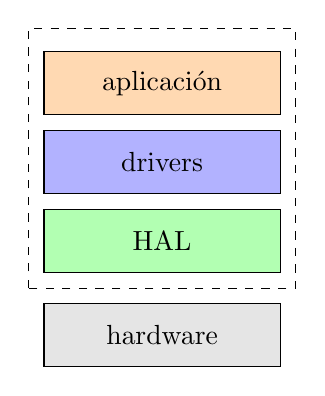
\begin{tikzpicture}
	% Define separated layers
	\node[draw, fill=orange!30, minimum width=3cm, minimum height=0.8cm] at (0, 2) {aplicación};
	\node[draw, fill=blue!30, minimum width=3cm, minimum height=0.8cm] at (0, 1.0) {drivers};
	\node[draw, fill=green!30, minimum width=3cm, minimum height=0.8cm] at (0, 0) {HAL};
	\node[draw, fill=gray!20, minimum width=3cm, minimum height=0.8cm] at (0, -1.2) {hardware};
	
	% Outline dashed box surrounding only the top three layers
	\draw[dashed] (-1.7, -0.6) rectangle (1.7, 2.7);
	\end{tikzpicture}
	\caption{Patrón de arquitectura de capas, obtenido a partir de presentaciones de clases de Ingeniería de Software \protect\footnotemark.}
	\label{fig:patroncapas}
\end{figure}
\footnotetext{Imagen obtenida de diapositiva de la materia Ingeniería de Software,  CESE, FIUBA, 2023.}

El patrón ``observar y reaccionar'', que se muestra en la figura \ref{fig:patronobservarreaccionar}, es la base del sistema de monitoreo. Su implementación en la capa de aplicación permitió la supervisión continua de los sensores y el procesamiento sistemático de los datos. El diseño implementó un mecanismo de notificación basado en el patrón de observador, donde los sensores funcionaron como sujetos observables, lo que generó eventos o cambios de estado. Por otro lado, los módulos de procesamiento y almacenamiento fueron diseñados como observadores, encargados de recibir y procesar las notificaciones emitidas por los sujetos observables.

\begin{figure}[H]
	\footnotesize
	\centering
	% Patron Obervar y reaccionar
	

\shorthandoff{>}
\begin{tikzpicture}[
node distance=0.5cm,
every node/.style={
	draw,
	rounded corners,
	minimum height=1cm,
	minimum width=2.5cm,
	align=center 
},
label/.style={    % Nuevo estilo para etiquetas
	draw=none,    % Sin borde
	minimum height=0cm,  % Sin altura mínima
	minimum width=0cm   % Sin ancho mínimo
}
]
% Definición de nodos
\node (observer) {proceso\\ observador};
\node[above=0.5cm of observer] (sensors) {sensores};
\node[right=2cm of observer] (analysis) {proceso de\\ análisis};
\node[right=2cm of analysis] (display) {proceso de\\ despliegue};
\node[above=0.5cm of display] (screen) {pantalla};
\node[below left=0.5cm and 0.5cm of analysis] (alarm) {proceso de\\ alarma};
\node[below right=0.5cm and 1cm of analysis] (reactor) {proceso reactor};
\node[below=of alarm] (alarmDevice) {alarma};
\node[below=of reactor] (otherDevice) {otro equipo};

% Conexiones
\draw[-latex] (sensors) -- (observer);
\draw[-latex] (observer) -- node[label, above] {valores de\\ sensor} (analysis);
\draw[-latex] (analysis) -- node[label, above] {valores a\\ desplegar} (display);
\draw[-latex] (display) -- (screen);
\draw[-latex] (analysis) -- (alarm);
\draw[-latex] (alarm) -- (alarmDevice);
\draw[-latex] (analysis) -- (reactor);
\draw[-latex] (reactor) -- (otherDevice);
\end{tikzpicture}
\shorthandon{>}
	\caption{Patrón arquitectónico: ``observar y reaccionar'' \protect\footnotemark.}
	\label{fig:patronobservarreaccionar}
\end{figure}
\footnotetext{Imagen obtenida de diapositiva de la materia Ingeniería de Software,  CESE, FIUBA, 2023.}

El tercer patrón implementado, ``segmentación de procesos'', estableció el flujo de datos entre los módulos del sistema. Un esquema de este patrón puede ser observado en la figura \ref{fig:patronsegmentacionprocesos}. Esta arquitectura definió etapas específicas para la adquisición, validación, procesamiento estadístico y almacenamiento de las mediciones. La segmentación aseguró la integridad de los datos mediante buffers intermedios entre etapas y mecanismos de verificación en cada transferencia. Esta implementación permitió el procesamiento secuencial de las mediciones y facilitó la detección de errores en el flujo de datos.

\begin{figure}[H]
	\centering
	\small
	% patron de segmentacion
		\shorthandoff{>}
		\begin{tikzpicture}[node distance=5cm, every node/.style={draw, rounded corners, minimum height=1.5cm, minimum width=2.2cm, align=center}]
			% Nodes
			\node (producer) {proceso\\ productor};
			\node[right of=producer] (buffer) {proceso\\ buffer};
			\node[right of=buffer] (consumer) {proceso\\ consumidor};
			\node[right=1cm of consumer, draw=none, minimum width=0.1cm] (ellipsis) {...};
			
			% Connections with labels outside of boxes
			\path[-latex] (producer) edge node[above, draw=none] {datos\\ producidos} (buffer);
			\path[-latex] (buffer) edge node[above, draw=none] {datos\\ consumidos} (consumer);
			\path[-latex] (consumer) edge (ellipsis);
		\end{tikzpicture}
		\shorthandon{>}
	\caption{ Patrón arquitectónico: “segmentación de procesos” \protect\footnotemark.}
	\label{fig:patronsegmentacionprocesos}
\end{figure}
\footnotetext{Imagen obtenida de diapositiva de la materia Ingeniería de Software,  CESE, FIUBA, 2023.}


\subsection{Integración de las estructuras y flujo de datos}

La figura \ref{fig:diagpatrones} presenta la integración de la arquitectura de software del sistema. La implementación estableció procesos interconectados para la gestión del flujo de datos, desde la adquisición en los sensores hasta el almacenamiento y transmisión de la información. Estos procesos incluyeron la validación de mediciones, el procesamiento estadístico, el almacenamiento local y la comunicación con sistemas remotos.

\begin{figure}[htpb]
	\centering
	\footnotesize
		
	\shorthandoff{<>} % Desactivar caracteres problemáticos
	
	
	\begin{tikzpicture}[ node distance=1cm]
	% Nodes
	%\draw[rounded corners] (0,0) rectangle (4,2);
	
	\node (observador) 
	[draw, rectangle, rounded corners, fill=blue!10!white, 
	align=center, yshift=2cm, xshift=0cm] 						
	{proceso\\ observador}; %\rotatebox{90}{\faMicrochip}};  
	
	\node (sensor1) 		
	[above left=of observador, draw, circle, fill=red!10!white, align=center, yshift=0.1cm, xshift=1cm] 	
	{\faSmog};
	
	\node (sensor2) 		
	[above=of observador, draw, circle, fill=red!10!white, align=center, yshift=-0.3cm, xshift=0.0cm] 	
	{ \faSmog};
	
	\node (sensor3)
	[above right=of observador, draw, circle, fill=red!10!white, align=center, yshift=0.1cm, xshift=-.80cm]
	{\faSmog};
	
	\node (rtc) 			
	[below =of observador, draw, circle, align=center,fill=red!10!white, yshift=0cm, xshift=0.0cm]  
	{\faClock[regular]};
	\node (sensorRTC) [below=of rtc,align=center, xshift=0 cm,yshift=1cm]     {\textbf{RTC} }; %\faCloudSunRain
	
	
	\node (tyh) 			
	[below  right=of observador, draw, circle, align=center,fill=red!10!white, yshift=0cm, xshift=-1.0cm]  {\faThermometerHalf};
	\node (sensorTyH) [below=of tyh, align=center, xshift=0.1 cm,yshift=1cm] 
	{\textbf{TyH} }; %\faCloudSunRain


	
	\node (sensores) [above =of sensor1,align=center, xshift=1 cm,yshift=-1cm]     {\textbf{sensores  \MPF} }; %\faCloudSunRain
	
	\node (aplicacion) 
	[right=2cm of sensores,align=center, xshift=-0.5 cm,yshift=0.2cm]     
	{\textbf{capa aplicación} }; %\faCloudSunRain
	
	\node (segmentacion) 		
	[right=of observador, draw, rectangle, rounded corners, fill=red!30!white, align=center, yshift=0cm, xshift=0cm] 						
	{ patrón \\ segmentación}	;
	
	\node (analisis) 		
	[right=of segmentacion, draw, rectangle, rounded corners, fill=blue!10!white, align=center, yshift=0cm, xshift=0cm] 						
	{proceso \\ de análisis};
	
	\node (despliegue) 		
	[right=of analisis, draw, rectangle, rounded corners, fill=blue!10!white, align=center, yshift=0cm, xshift=0cm] 						
	{proceso \\ despliegue};
	
	\node (alarma)
	[below left=of analisis, draw, rectangle, rounded corners, fill=blue!10!white, align=center, yshift=0cm, xshift=1cm] 						
	{proceso \\ alarma};
	
	\node (reactor) 		
	[below right=of analisis, draw, rectangle, rounded corners, fill=blue!10!white, 	align=center, yshift=0cm, xshift=0cm] 						
	{ proceso \\ reactor};
	
	\node (servidor) 		
	[below=0.4 cm of reactor,  align=center, yshift=0cm, xshift=0cm] 						
	{módulo\\inalámbrico \faWifi}; % https://www.ipgp.fr/~moguilny/LaTeX/fontawesome5Icons.pdf
	
	\node (led) 		
	[below=0.5cm of alarma,  align=center, yshift=0cm, xshift=0cm] 						
	{LED \faLightbulb};
	
	\node (memoria) 		
	[above=of despliegue,  align=center, yshift=0cm, xshift=0cm] 						
	{memoria \faSdCard };
	
	% Bounding Box
	\begin{scope}[on background layer]
	\node(aplicacion)[fill=orange!15,  draw, rectangle, rounded corners, fit=(aplicacion)(sensor1) (sensor2) (sensor3) (sensores) (despliegue) (rtc) (servidor) (alarma)] {};
	\node(driver)[below=of aplicacion,fill=blue!15,  draw, rectangle, rounded corners,
	minimum width=11cm, minimum height=0.8cm, , yshift=0.8cm, xshift=0cm]{capa drivers} ;
	\node(hal)[below=of driver,fill=green!10,  draw, rectangle, rounded corners,
	minimum width=11cm, minimum height=0.8cm, yshift=0.8cm]{capa HAL} ;
	\node(hardware)[below=of hal,fill=gray!10,  draw, rectangle, rounded corners,
	minimum width=11cm, minimum height=0.8cm,  yshift=0.5cm]{Hardware} ;
	\node[draw, dashed, fit=(aplicacion) (driver) (hal), inner sep=8pt, rounded corners] (box) {};
	\end{scope}
	
	% Arrows
	\draw[-] (observador) -- (sensor1);
	\draw[-] (observador) -- (sensor2);
	\draw[-] (observador) -- (sensor3);
	\draw[->] (observador) -- (segmentacion);
	\draw[->] (segmentacion) -- (analisis);
	\draw[->] (analisis) -- (despliegue);
	\draw[->] (despliegue) -- (memoria);
	\draw[->] (analisis) -- (reactor);
	\draw[->] (reactor) -- (servidor); % \faWifi
	\draw[->] (analisis) -- (alarma);
	\draw[->] (alarma) -- (led);
	\draw[-] (rtc) -- (observador);
	\draw[-] (tyh) -- (observador);
	
	\end{tikzpicture}
		\shorthandon{<>} 
	\caption{Arquitectura de bloques de los componentes del software.}
	\label{fig:diagpatrones}
\end{figure}


\subsection{Procesos principales}
Para el software se implementaron tres procesos fundamentales para la gestión de datos:

\subsubsection{Proceso observador}

Este proceso constituyó el punto de entrada del sistema, lo que permitió la adquisición de datos desde los sensores de temperatura, humedad, \MPF y el RTC. La implementación estableció un sistema de muestreo configurable con intervalos desde 10 minutos hasta 24 horas, lo que permitió adaptar el monitoreo a diferentes requisitos. Cada medición incorporó una marca temporal del RTC para asegurar la trazabilidad de los datos.

\subsubsection{Proceso de análisis}

El núcleo central del sistema recibió los datos del proceso observador mediante un buffer intermediario. Este módulo implementó las calibraciones, ejecutó cálculos estadísticos y validó la integridad de la información. El procesamiento incluyó el cálculo de promedios móviles, desviaciones estándar y la detección de valores atípicos para determinar la calidad del aire.

\subsubsection{Procesos de salida}

La arquitectura implementó tres componentes especializados:
\begin{itemize}
	\item Proceso de despliegue: gestionó el registro en memoria microSD, en datos con estructuras temporales de 10 minutos, 1 hora y 24 horas.
	\item Proceso reactor: manejó la transmisión de los datos hacia el módulo inalámbrico hacia un servidor remoto mediante protocolos estandarizados.
	\item Proceso de alarma: controló indicadores LED para proporcionar retroalimentación visual sobre el estado del sistema.
\end{itemize}

\subsection{Interfaces y comunicaciones}

El sistema implementó múltiples protocolos de comunicación para interactuar con sus componentes periféricos. La comunicación con los sensores \MPF se estableció mediante UART, mientras que la interfaz con el RTC utilizó el protocolo \IIC. El almacenamiento de los datos en la memoria microSD se realizó a través del protocolo SPI. La transmisión inalámbrica de datos empleó una interfaz UART adicional, y el control de señalización mediante LED se gestionó a través de GPIO.

La gestión de energía implementó un sistema de conmutación automática para mantener la operatividad ante fallos en el suministro eléctrico principal. El diseño incorporó un modo de bajo consumo que se activó cuando el sistema operó con batería de respaldo. Esto permitió reducir el consumo energético mediante la desactivación selectiva de periféricos no críticos, por ejemplo, el módulo de comunicación inalámbrica. Esta implementación incremento el tiempo de funcionamiento de las mediciones durante interrupciones eléctricas.


\section{Detalle de los componentes y responsabilidades}

La implementación del sistema estableció una arquitectura de procesos interconectados, donde cada componente ejecutó funciones específicas en el flujo de datos. Esta organización permitió la adquisición desde los sensores, el procesamiento de las mediciones y su posterior almacenamiento, tanto en la memoria local como en el servidor remoto.

Los procesos implementados se alinearon con los patrones arquitectónicos descritos, como se ilustra en las figuras \ref{fig:diagpatrones} y \ref{fig:diagsegmentacion}. La arquitectura integró seis componentes principales: el proceso observador para la adquisición de datos, el buffer intermediario para la gestión temporal, el proceso de análisis para la validación estadística, el proceso de despliegue para el almacenamiento local, el proceso reactor para la transmisión remota y el proceso de alarma para la señalización del estado del sistema.

\begin{figure}[htpb]
	\centering
	\footnotesize
		\shorthandoff{<>} % Desactivar caracteres problemáticos
	
	
	\begin{tikzpicture}[ node distance=2cm]
	% Nodes
	%\draw[rounded corners] (0,0) rectangle (4,2);
	
	\node (observador) 
	[draw, rectangle, rounded corners, fill=blue!10!white, 
	align=center, yshift=2cm, xshift=0cm] 						
	{proceso \\ observador}; %\rotatebox{90}{\faMicrochip}};  
	
	
	\node (buffer) 		
	[right=of observador,  draw, rectangle, rounded corners, fill=blue!10!white, align=center, yshift=0cm, xshift=1cm] 						
	{ proceso \\ buffer};
	
	\node (aplicacion) 
	[above =of observador,align=left, xshift=0.5 cm,yshift=-0.3cm]     
	{\textbf{capa aplicación} }; %\faCloudSunRain
	
	\node (segmentacion) 
	[above =of buffer,align=left, xshift=0 cm,yshift=-1.2cm]     
	{\textbf{patrón de segmentación} }; %\faCloudSunRain
	
	
	\node (analisis) 		
	[right=of buffer, draw, rectangle, rounded corners, fill=blue!10!white, align=center, yshift=0cm, xshift=1cm] 						
	{proceso \\ de análisis};
	
	% Nodos invisibles para las etiquetas de las flechas
	\node (etiqueta1) [left=of buffer, yshift=1.6cm, xshift=-0.2cm] {};
	\node (etiqueta2) [right=of buffer, yshift=1.6cm, xshift=0.2cm] {};
	
	
	
	
	% Arrows
	\draw[->] (observador) -- (buffer) 
	node[above, align=center, midway] 
	{datos \\ producidos};
	
	\draw[->] (buffer) -- (analisis) 
	node[above, align=center, midway] 
	{datos \\ consumidos};
	
	% Ajuste del cuadro segmentado para incluir las etiquetas
	\begin{scope}[on background layer]
	\node(aplicacion)
	[fill=orange!10,  draw, rectangle, inner sep=10pt, rounded corners, fit=(aplicacion) (observador) (analisis)(etiqueta2) ] {};
	\node[draw, dashed, fill=red!30!white, fit=(buffer) (etiqueta1) (etiqueta2), inner sep=4pt, rounded corners] (box) {};
	\end{scope}
	
	\end{tikzpicture}
		\shorthandon{<>} % Reactivar caracteres problemáticos
	\caption{Detalle con el patrón de segmentación del software.}
	\label{fig:diagsegmentacion}
\end{figure}



\subsection{Proceso observador:}

Este proceso se empleo durante la captura de datos,  los sensores de \MPF y el Reloj de Tiempo Real (RTC). Su tarea consistió en la recolección continua de información sobre la concentración de partículas en el aire, junto con marcas temporales para cada conjunto de datos. Posteriormente, estos datos son encaminados hacia la etapa de preprocesamiento (proceso buffer - segmentación de procesos).

Este proceso está encargado de solicitar y recabar datos de los sensores de \MPF en intervalos que pueden variar desde un minuto hasta horas, según la configuración establecida. Esta flexibilidad en la programación permite configurar la toma de muestras, adecuándose a diferentes necesidades de monitoreo y características específicas de cada sensor. Adicionalmente, el módulo se encargará de obtener del RTC y escribir en cada registro una marca temporal del dato. Una vez recolectados, estos datos son transmitidos al siguiente eslabón en el proceso, el \textit{``proceso buffer''}, para su posterior tratamiento.


\subsection{Proceso buffer:} 

El proceso buffer es un componente del patrón de segmentación, responsable del acondicionamiento y almacenamiento temporal de los datos. La implementación estableció una estructura intermedia entre el proceso observador y el proceso de análisis.

El diseño implementó tres niveles de almacenamiento temporal: un buffer de alta frecuencia con retención de 10 minutos para datos instantáneos; un buffer horario para el cálculo de promedios móviles; y un buffer diario para la generación de estadísticas de 24 horas. Este proceso recibió los datos del proceso observador, ejecutó la validación preliminar y el formateo de la información, para su posterior transferencia al proceso de análisis. La tabla \ref{tab:buffer_estructura} presenta la organización de los datos en cada nivel de almacenamiento.

\begin{table}[htbp]
	\centering
	\small
	\caption{Ejemplo de estructura de datos.}
	\label{tab:buffer_estructura}
	% ejemplos estructura de datos
\begin{tabular}{lcc}
	\toprule
	\textbf{Atributo} & \textbf{Tipo de dato} & \textbf{Formato} \\
	\midrule
	idsensor    & int   & - \\
	fecha-hora  & int   & AAMMDDHHMM \\
	frecuencia  & int   & - \\
	\MPF        & float & - \\
	temperatura & int   & - \\
	humedad     & int   & - \\
	\bottomrule
\end{tabular}
\end{table}                           


\subsection{Proceso de análisis}
El proceso de análisis implementó el cálculo numérico y la validación estadística de los datos provenientes del buffer. Las operaciones incluyeron la corrección de las concentraciones mediante parámetros de calibración y el cálculo de estadísticos para diferentes intervalos temporales (10 minutos, 1 hora y 24 horas).

Se aplicaron métodos numéricos que permitió estimar la calidad de las mediciones mediante el cálculo de valores centrales y de dispersión. Esta incorporó algoritmos para la detección de valores atípicos y la evaluación de la concordancia entre los tres sensores de \MPF. Este procesamiento generó índices de confiabilidad para cada medición y activó alarmas ante la detección de anomalías en el funcionamiento de los sensores.

\subsection{Proceso de despliegue}
El proceso de despliegue implementó la gestión del almacenamiento de datos en la memoria microSD. Este módulo recibió la información procesada del proceso de análisis y ejecutó las operaciones de escritura en el sistema de archivos.

La implementación estableció una estructura jerárquica de almacenamiento con tres niveles temporales: registros de 10 minutos, promedios horarios y resúmenes diarios. El sistema generó archivos independientes para cada período. Incorpora metadatos que identificaron el origen y características de las mediciones. Esta organización permitió la trazabilidad de los datos y facilitó su posterior procesamiento.

\subsection{Proceso reactor}

El proceso reactor implementó la comunicación de datos entre el sistema y un servidor remoto mediante el módulo Wi-Fi. Este componente estableció la interfaz entre el proceso de análisis y la transmisión inalámbrica de información.

Se incorporarón tres funciones principales: la gestión de la configuración de red inalámbrica, el establecimiento del protocolo de transferencia de archivos (FTP), y la transmisión de datos procesados. El sistema transmitió los registros temporales organizados en intervalos de 10 minutos, promedios horarios y resúmenes diarios. Cada paquete de datos incluyó metadatos de identificación que especificaron el origen y características de las mediciones transmitidas.

\subsection{Proceso de alarma}
El proceso de alarma implementó la señalización visual del estado operativo del sistema mediante un indicador LED. Este módulo procesó los códigos de estado generados por los distintos componentes y tradujo esta información en patrones específicos de señalización luminosa.

Se estableció una codificación basada en frecuencias de parpadeo del LED para indicar diferentes estados operativos: funcionamiento normal, fallos en sensores, errores de comunicación y estados del sistema. Esta interfaz visual proporcionó retroalimentación inmediata sobre el estado del instrumento al usuario.

\subsection{Módulo de energía}
El módulo de energía implementó la gestión y distribución de alimentación eléctrica para todos los componentes del sistema. La arquitectura estableció un sistema de conmutación automática entre la fuente principal de \SI{220}{\volt} y una batería de respaldo.

La incorporó dos modos de operación: normal y bajo consumo. El modo normal operó con la fuente principal, mientras que el modo de bajo consumo se activó de manera automática ante interrupciones en el suministro eléctrico. Este último redujo el consumo mediante la desactivación selectiva de componentes no críticos, lo que permitió mantener las funciones esenciales del sistema durante períodos limitados de operación con batería.

\section{Responsabilidades de las interfaces periféricas}

Descripción de las principales funcionalidades con los componentes y sensores periféricos.

\subsection{Sensores \MPF}
La interfaz con los sensores de \MPF constituyó el componente principal para la adquisición de datos de concentración de material particulado. Se estableció la comunicación mediante el protocolo UART, seleccionado por sus características de transmisión serie asíncrona y compatibilidad con los sensores SPS30.

El proceso observador gestionó la operación de los sensores mediante una secuencia definida de comandos: inicialización, configuración de parámetros de medición, adquisición de datos y verificación de estado. Este protocolo de comunicación permitió la obtención sistemática de mediciones de concentración de \MPF con una resolución temporal programable.

\subsection{Reloj de tiempo real RTC}

Con los datos entregados por el RTC DS3231 se implementó la base de tiempo del sistema, necesario para el registro temporal de las mediciones. El proceso observador gestionó la comunicación con este dispositivo mediante el protocolo \IIC, seleccionado por su compatibilidad y eficiencia en la transmisión de datos temporales.

Se incorporaron dos funciones principales: la sincronización periódica del sistema y el etiquetado temporal de las mediciones de \MPF. Esta interfaz proporcionó marcas de tiempo con precisión de \SI{\pm2}{\ppm}.

\subsection{Almacenamiento microSD}

Se integró un módulo de almacenamiento con memoria microSD para el registro local de datos. El proceso de despliegue gestionó las operaciones de escritura y lectura mediante el protocolo SPI, que operó a una frecuencia de \SI{42}{\mega\hertz}.

Se incorporó el sistema de archivos FAT32 y estableció un buffer de escritura de \SI{512}{\byte} para optimizar las operaciones de almacenamiento. Esta interfaz permitió el registro estructurado de las mediciones.
	
\subsection{Módulo de conexión inalámbrica}

El software integró la comunicación con un servidor remoto mediante el módulo Wi-Fi ESP8266. El proceso reactor estableció la interfaz entre el sistema de medición y la transmisión de datos.

Se incorporó tres funciones principales: la configuración de la conexión Wi-Fi, la gestión del protocolo FTP para la transferencia de archivos, y la comunicación UART con el módulo ESP8266 a \SI{115200}{\baud}. Esta arquitectura permitió la transmisión automática de los datos almacenados hacia el servidor remoto mediante una conexión TCP/IP.
	
	
\subsection{Señal de estado LED}

Se incorporó un indicador visual mediante LED para la señalización del estado operativo. El proceso de alarma gestionó la codificación de estados del sistema mediante patrones de parpadeo predefinidos.

Se utilizó un puerto GPIO configurado en modo PWM para el control del LED. Esta interfaz estableció diferentes frecuencias de parpadeo para señalizar distintas condiciones operativas: funcionamiento normal; errores en sensores; fallos de comunicación; y estados de la alimentación. Este método proporcionó retroalimentación inmediata sobre el estado del sistema al usuario.
	
	
\subsection{Gestión de energía}
El módulo de gestión de energía implementó un sistema de monitorización del suministro eléctrico mediante un puerto GPIO configurado en modo lectura. Este componente supervisó el estado de la alimentación principal y controló la conmutación automática hacia la batería de respaldo.

Se definieron dos funciones principales: la detección de interrupciones en el suministro de \SI{220}{\volt} y la activación del modo de bajo consumo. El sistema utilizó el estado binario del GPIO para determinar la fuente de alimentación activa y ejecutar la transición entre modos de operación, lo que aseguró la continuidad del monitoreo ante fallos en el suministro eléctrico.
	
	

\section{Implementación de protocolos}

La integración de protocolos de comunicación en el sistema de medición de \MPF estableció las interfaces entre módulos y periféricos. Se incorporaron protocolos estandarizados para asegurar la confiabilidad y eficiencia en la transferencia de datos.

\subsection{Protocolo UART para sensores de \MPF}
La comunicación con los sensores SPS30 se implementó mediante una interfaz UART en configuración maestro-esclavo. El protocolo estableció los siguientes parámetros operativos:

\begin{itemize}
	\item Velocidad de comunicación: \SI{100}{\kilo\hertz}.
	\item Direccionamiento: asignación de dirección única por sensor (0x69).
	\item Buffer de recepción: \SI{32}{\byte} para datos de concentración.
	\item Tiempo máximo de transacción: \SI{30}{\milli\second}.
\end{itemize}

La secuencia de comunicación sigue el  patrón de la figura \ref{fig:i2c_sequence}.

\begin{figure}[h]
	\centering
	\small
	% secuencia de comunicacion SPS30 
	\shorthandoff{>}
	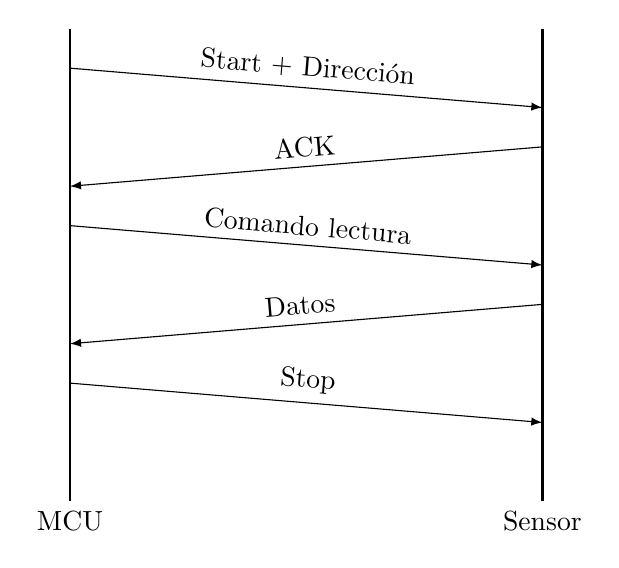
\begin{tikzpicture}[
	node distance=2cm,
	every node/.style={align=center},
	label/.style={draw=none}
	]
	% Líneas de tiempo verticales
	\draw[thick] (0,0) -- (0,-6) node[below] {MCU};
	\draw[thick] (6,0) -- (6,-6) node[below] {Sensor};
	
	% Mensajes
	\draw[-latex] (0,-0.5) -- (6,-1) node[midway, above, sloped] {Start + Dirección};
	\draw[-latex] (6,-1.5) -- (0,-2) node[midway, above, sloped] {ACK};
	\draw[-latex] (0,-2.5) -- (6,-3) node[midway, above, sloped] {Comando lectura};
	\draw[-latex] (6,-3.5) -- (0,-4) node[midway, above, sloped] {Datos \MPF};
	\draw[-latex] (0,-4.5) -- (6,-5) node[midway, above, sloped] {Stop};
	\end{tikzpicture}
	\shorthandon{>}
	\caption{Secuencia de comunicación UART con sensor SPS30.}
	\label{fig:i2c_sequence}
\end{figure}

\subsection{Protocolo SPI para almacenamiento}
Se aplicó el protocolo SPI de comunicación con la memoria microSD. El diseño incorporó las siguientes especificaciones técnicas:

\begin{itemize}
	\item Frecuencia de operación: \SI{42}{\mega\hertz} en modo maestro.
	\item Sistema de archivos: FAT32 con sectores de \SI{512}{\byte}.
	\item Transferencia de datos: DMA para optimización de recursos.
	\item Buffer circular: \SI{512}{\byte} para gestión de escritura.
\end{itemize}

\subsection{UART para comunicación inalámbrica}
La implementación de la comunicación con el módulo ESP8266 estableció una interfaz UART con los siguientes parámetros operativos:
\begin{itemize}
	\item Velocidad de transmisión: \SI{115200}{\baud}.
	\item Control de flujo: señales hardware RTS/CTS.
	\item Buffer de transmisión: \SI{256}{\byte}.
	\item Tiempo de espera máximo: \SI{100}{\milli\second}.
\end{itemize}
La capa de aplicación implementó los siguientes mecanismos de control:
\begin{itemize}
	\item Establecimiento de conexión mediante handshaking.
	\item Sistema de retransmisión automática ante fallos.
	\item Verificación de integridad mediante CRC-16.
	\item Estructura de trama con campos de cabecera y cola.
\end{itemize}

\subsection{GPIO para control y monitoreo}
Se estableció tres funciones principales para la puesta en funcionamiento de las interfaces GPIO :
\begin{itemize}
	\item Señalización visual: control del LED mediante modulación PWM.
	\item Supervisión energética: detección del estado de alimentación.
	\item Control de energía: gestión del modo de bajo consumo.
\end{itemize}
\subsection{Gestión de errores y recuperación}
El sistema implementó mecanismos de protección y recuperación ante fallos de comunicación:
\begin{itemize}
	\item Sistema de temporización: límites de tiempo para cada transacción.
	\item Recuperación automática: reinicialización de periféricos ante errores.
	\item Sistema de respaldo: buffer temporal para datos críticos.
	\item Trazabilidad: registro de eventos de error en memoria no volátil.
\end{itemize}

\subsection{Optimización del rendimiento}
Al instrumento se le incorporó mecanismos específicos para optimizar la eficiencia del sistema:
\begin{itemize}
	\item Transferencia de datos: DMA para operaciones críticas.
	\item Gestión de eventos: sistema de interrupciones para respuesta inmediata.
	\item Administración de memoria: buffers circulares para gestión eficiente.
	\item Planificación: esquema de prioridades para tareas de comunicación.
\end{itemize}

El diseño modular permitió el mantenimiento y actualización independiente de cada protocolo, mientras que los mecanismos de optimización aseguraron un uso eficiente de los recursos del microcontrolador.

	
\section{Ajuste y calibración de sensores y transmisores}
Se estableció un proceso sistemático de calibración y ajuste del sistema de medición de \MPF para asegurar la precisión y trazabilidad de las mediciones. Este procedimiento consideró las características específicas de los sensores SPS30 y las condiciones ambientales de operación.
\subsection{Calibración de sensores \MPF}
El protocolo de calibración se implementó en dos etapas principales:
\begin{enumerate}
	\item Calibración de fábrica: Los sensores incorporaron una calibración inicial contra instrumentos de referencia:
	\begin{itemize}
		\item Fotómetro TSI DustTrak™ DRX 8533: validación gravimétrica.
		\item Espectrómetro óptico TSI OPS 3330: caracterización de distribución de partículas.
	\end{itemize}
	\item Calibración en campo: La implementación requirió ajustes específicos según condiciones locales:

	\begin{itemize}
		\item Correlación con monitor Beta de referencia.
		\item Factor de corrección por humedad relativa.
		\item Compensación por temperatura ambiente.
	\end{itemize}
\end{enumerate}


\subsection{Modelo de corrección}
Se incorporó un modelo de corrección lineal para el ajuste de las mediciones:
\begin{equation}
C_{corregida} = a \cdot C_{medida} + b \cdot H + c \cdot T + d
\end{equation}
Donde las variables representan:
\begin{itemize}
	\item $C_{corregida}$: concentración ajustada (\si{\micro\gram\per\cubic\meter}).
	\item $C_{medida}$: concentración del sensor SPS30.
	\item $H$: humedad relativa (\%).
	\item $T$: temperatura (\si{\celsius}).
	\item $a$, $b$, $c$, $d$: coeficientes determinados  de manera experimental.
\end{itemize}

\subsection{Procedimiento de calibración}
El procedimiento de calibración en campo estableció cinco etapas secuenciales:
\begin{enumerate}
	\item Acondicionamiento inicial: período de estabilización de 24 horas.
	\item Adquisición de datos: mediciones simultáneas con monitor Beta de referencia.
	\item Procesamiento estadístico: determinación de coeficientes mediante regresión lineal.
	\item Verificación: validación con conjunto de datos independiente.
	\item Programación: actualización del firmware con factores de corrección.
\end{enumerate}


\subsection{Validación y control de calidad}
Se ejecutaron mecanismos automáticos para el aseguramiento de la calidad de las mediciones:
\begin{itemize}
	\item Sistema de detección de valores atípicos.
	\item Validación cruzada entre los tres sensores redundantes.
	\item Monitoreo continuo de variables ambientales.
	\item Sistema de notificación para recalibración programada.
\end{itemize}
\subsection{Mantenimiento y recalibración}
El protocolo de mantenimiento estableció un cronograma sistemático de verificación:
\begin{itemize}
	\item Validación trimestral con monitor Beta de referencia.
	\item Ciclo automático de limpieza cada \SI{168}{\hour}.
	\item Recalibración integral anual.
	\item Compensación de la deriva temporal mediante ajuste de coeficientes.
\end{itemize}

Esta implementación sistemática de calibración y control busca asegurar la estabilidad y precisión de las mediciones a largo plazo. La arquitectura con tres sensores permitió la validación continua de datos y la detección temprana de desviaciones en el sistema de medición.

%\section{Análisis del software}
% 
%La idea de esta sección es resaltar los problemas encontrados, los criterios utilizados y la justificación de las decisiones que se hayan tomado.
%
%Se puede agregar código o pseudocódigo dentro de un entorno lstlisting con el siguiente código:
%
%\begin{verbatim}
%\begin{lstlisting}[caption= "un epígrafe descriptivo"]
%	las líneas de código irían aquí...
%\end{lstlisting}
%\end{verbatim}
%
%A modo de ejemplo:
%
%\begin{lstlisting}[label=cod:vControl,caption=Pseudocódigo del lazo principal de control.]  % Start your code-block
%
%#define MAX_SENSOR_NUMBER 3
%#define MAX_ALARM_NUMBER  6
%#define MAX_ACTUATOR_NUMBER 6
%
%uint32_t sensorValue[MAX_SENSOR_NUMBER];		
%FunctionalState alarmControl[MAX_ALARM_NUMBER];	//ENABLE or DISABLE
%state_t alarmState[MAX_ALARM_NUMBER];						//ON or OFF
%state_t actuatorState[MAX_ACTUATOR_NUMBER];			//ON or OFF
%
%void vControl() {
%
%	initGlobalVariables();
%	
%	period = 500 ms;
%		
%	while(1) {
%
%		ticks = xTaskGetTickCount();
%		
%		updateSensors();
%		
%		updateAlarms();
%		
%		controlActuators();
%		
%		vTaskDelayUntil(&ticks, period);
%	}
%}
%\end{lstlisting}




%	%!TEX root = ../T1_Gomez_Luis_.tex

\chapter{Ensayos y resultados} % Main chapter title
\label{Chapter4} % For referencing this chapter elsewhere, use \ref{Chapter4}

%----------------------------------------------------------------------------------------
%	SECTION 1
%----------------------------------------------------------------------------------------

Este capítulo presenta la evaluación del sistema de medición de \MPF desarrollado, abarcando validación técnica, caracterización metrológica y rendimiento operativo. Se analizaron los resultados de las pruebas realizadas sobre el diseño electrónico, el sistema de alimentación y la implementación del software mediante un banco de pruebas estructurado. Se evalúa la calidad metrológica del instrumento a través del análisis de correlación entre los tres sensores redundantes y su comparación con equipos de referencia. La caracterización operativa incluye la verificación de la completitud de datos adquiridos, el análisis de patrones temporales de concentración, y la respuesta del instrumento ante un evento controlado de alta contaminación. Los resultados obtenidos, presentados mediante análisis estadístico y visualizaciones temporales, muestran que el sistema alcanza los niveles de confiabilidad y precisión requeridos para aplicaciones de monitoreo ambiental urbano.

\section{Banco de prueba} 


%	1	Descripción de las herramientas utilizadas para probar el dispositivo	Imágenes de equipos de prueba	Métodos de prueba y sus parámetros


El banco de pruebas se estructuró en cuatro categorías funcionales complementarias: instrumentación electrónica, validación metrológica, verificación de hardware y pruebas de software.

La instrumentación electrónica comprendió equipos para la caracterización y diagnóstico de los circuitos. Se utilizó un analizador lógico de \SI{24}{\mega\hertz} con 8 canales para la verificación de protocolos de comunicación (\IIC, SPI, UART), lo que permitió monitorizar en tiempo real las transacciones de datos entre el microcontrolador y los periféricos. Para el análisis de señales de alta frecuencia, se empleó un osciloscopio FNIRSI1014D de \SI{100}{\mega\hertz}, que facilitó la medición de tiempos de respuesta, detección de interferencias y verificación de integridad de señales críticas. Las mediciones de parámetros eléctricos se realizaron con un multímetro digital TMT460012, con resolución de \SI{0.01}{\milli\volt} para tensión y \SI{0.1}{\micro\ampere} para corriente. La alimentación controlada del sistema durante las pruebas se implementó mediante una fuente regulada Jesverty SPS-3005 con rango de \SIrange{0}{30}{\volt} y capacidad de corriente de \SI{5}{\ampere}.

Para la validación metrológica, las mediciones de \MPF se contrastaron con un instrumento de referencia Grimm y equipo certificado por su alta precisión (\SI{\pm2}{\percent}) en el análisis óptico de partículas atmosféricas dentro del rango de \SIrange{0.3}{10}{\micro\meter}. Esta comparación se realizó en dos escenarios: bajo condiciones controladas de laboratorio y en ambiente real, lo que expone a los sensores a las condiciones atmosféricas urbanas durante un período de 72 horas. Este enfoque dual permitió determinar tanto la exactitud y precisión del instrumento como su comportamiento en condiciones operativas reales.

La verificación del hardware se efectuó mediante un proceso sistemático que incluyó la comprobación del cumplimiento de las reglas de diseño de circuito impreso utilizó las herramientas integradas en KiCad. Este proceso verificó parámetros críticos como anchos de pista, distancias mínimas entre elementos y diámetros de vías. Adicionalmente, componentes  como inductores, capacitores y resistencias se caracterizaron individualmente con un medidor LCR-P1 de FNIRSI, que proporcionó datos  sobre sus propiedades eléctricas y tolerancias reales, lo que permite validar que sus valores se encontraban dentro de los márgenes establecidos para garantizar el funcionamiento correcto del circuito.

Las pruebas de software implementaron metodologías de validación mediante el framework Ceedling, que permitió la automatización de pruebas unitarias en lenguaje C. Esta aproximación posibilitó la evaluación independiente de cada módulo del firmware, facilitó la detección temprana de errores lógicos o de implementación. La integración de las herramientas Unity y CMock dentro del framework proporcionó capacidades para la creación de objetos simulados (\textit{mocks}) y aserciones específicas para validar el comportamiento esperado de las funciones. La verificación de comunicaciones se complementó con un terminal UART Cutecom, configurado a \SI{115200}{\baud}, para la inspección detallada de los datos transmitidos entre el sistema y los dispositivos periféricos, lo que facilitó la verificación del cumplimiento de los protocolos establecidos.

Las tablas \ref{tab:pruebas} y  \ref{tab:pruebas2} presentan un resumen  de los instrumentos empleados en el banco de pruebas. Esta detalla las características técnicas y función específica en el proceso de validación.





%\section{Pruebas funcionales del hardware}
%\label{sec:pruebasHW}

%La idea de esta sección es explicar cómo se hicieron los ensayos, qué resultados se obtuvieron y analizarlos.




\section{Evaluación del software}
%	3	Evaluación del rendimiento del hardware y herramientas empleadas para su evaluación	Fotos del prototipo final	Tabla con herramientas empleadas


La validación del sistema de medición de \MPF se enfocó en garantizar la precisión y confiabilidad del subsistema de análisis, identificado como componente crítico con una importancia relativa del 24\% según los criterios de diseño establecidos. Este componente procesa los datos provenientes de los sensores ópticos y realiza los cálculos estadísticos necesarios para determinar las concentraciones del contaminante.

\subsection{Metodología de pruebas de software}

Se implementó el \textit{Método del Árbol de Clasificación} (CTM) como estrategia principal para el diseño y ejecución de los casos de prueba. Esta técnica permitió una cobertura  y sistemática de los posibles escenarios de operación, lo que facilita la identificación de errores potenciales en el tratamiento de datos. El proceso consistió en cuatro etapas secuenciales:

\begin{enumerate}
	\item Definición de clases de equivalencia: se estableció categorías para los tipos de datos de entrada, lo que incluyó concentraciones dentro de los límites operativos (\SIrange{0.5}{500}{\micro\gram\per\cubic\meter}), valores por debajo del límite mínimo de cuantificación, mediciones que exceden el límite máximo de linealidad y casos atípicos como valores negativos o nulos.
	
	\item Construcción del árbol de clasificación: se desarrolló una estructura jerárquica que representa las diferentes clases de equivalencia y las relaciones entre ellas, lo que permitió la identificación de combinaciones específicas de condiciones para cada caso de prueba.
	
	\item Derivación de casos de prueba: a partir del árbol de clasificación, se identificó cinco escenarios representativos que abarcan las principales condiciones de operación y casos límite del sistema.
	
	\item Ejecución y análisis de resultados: se utilizó el framework Ceedling, junto con las herramientas Unity y CMock, para implementar y automatizar la ejecución de las pruebas unitarias.
\end{enumerate}

\subsection{Casos de prueba implementados}

Se desarrollaron cinco casos  para evaluar la función \texttt{calculateAverage} de la API \texttt{ParticulateDataAnalyzer}, responsable del cálculo del promedio de concentraciones de MP$_{2,5}$ bajo diferentes condiciones:

\begin{table}[h]
	\centering
	\small
	\caption{Resumen de los casos de prueba aplicados al subsistema de análisis.}
	\label{tab:casos-prueba-software}
	\begin{tabular}{c p{4.5cm} p{4.5cm} c }
		\hline
		\textbf{Test} & \textbf{Escenario} & \textbf{Objetivo} & \textbf{Resultado} \\
		\hline
		1 & Valores dentro del rango con algunos por debajo del límite de cuantificación & Verificar exclusión correcta de valores $< \SI{0.5}{\micro\gram\per\cubic\meter}$ & \SI{302.5}{\micro\gram\per\cubic\meter} \\
		
		2 & Datos válidos con algunos valores por encima del máximo y negativos & Comprobar manejo adecuado de valores fuera de rango superior y negativos & \SI{286.07}{\micro\gram\per\cubic\meter} \\
		
		3 & Arreglo completo de datos nulos & Validar respuesta ante ausencia total de datos válidos & $-999$ \\
		
		4 & Todos los valores dentro del rango permitido & Confirmar cálculo correcto con datos completamente válidos & \SI{316.67}{\micro\gram\per\cubic\meter} \\
		
		5 & Arreglo sin datos válidos (todos bajo límite) & Verificar comportamiento con datos insuficientes para cálculo & $-999$ \\
		\hline
	\end{tabular}
\end{table}

El caso de prueba 1 evaluó el procesamiento de un conjunto de datos donde la mayoría se encontraba dentro del rango operativo, lo que incluyó valores ligeramente por debajo del límite inferior de cuantificación (\SI{0.4}{\micro\gram\per\cubic\meter} y \SI{0.3}{\micro\gram\per\cubic\meter}). Esta prueba verificó que el sistema excluyera correctamente estos valores del cálculo del promedio y utilizara solo los 16 valores válidos restantes.

El caso 2 analizó el manejo de valores extremos, lo que incorporó tanto concentraciones negativas (\SI{-480}{\micro\gram\per\cubic\meter}) como mediciones superiores al límite máximo de linealidad (\SI{590}{\micro\gram\per\cubic\meter} y \SI{895}{\micro\gram\per\cubic\meter}). Esta prueba fue particularmente significativa para validar la robustez del sistema ante lecturas anómalas o errores de medición.

Los casos 3 y 5 evaluaron situaciones límite donde no existían datos válidos para el cálculo, ya sea por un arreglo completamente vacío o con datos por debajo del umbral mínimo de cuantificación. Ambos casos verificaron que el sistema respondiera adecuadamente con un valor de error predefinido ($-999$), lo que señaló la imposibilidad de realizar el cálculo.

El caso 4 representó un escenario ideal con todos los valores dentro del rango operativo permitido, lo que verificó la precisión del cálculo bajo condiciones óptimas de funcionamiento.

\subsection{Implementación de las pruebas}

Las pruebas se codificaron con el framework Ceedling, que integra las herramientas Unity y CMock para la automatización de pruebas unitarias en lenguaje C (ver figura \ref{fig:resultados-pruebas}). Cada caso de prueba se implementó como una función independiente que preparaba los datos de entrada, ejecutaba la función bajo evaluación y verificaba que el resultado correspondiera al valor esperado mediante aserciones.

La función \texttt{calculateAverage} evaluada realiza el procesamiento de un arreglo de valores flotantes que representan concentraciones de \MPF, con los siguientes pasos:

\begin{enumerate}
	\item Verifica si el arreglo está vacío mediante la función \texttt{isArrayEmpty}.
	\item Inicializa variables para sumatoria y conteo de valores no válidos.
	\item Recorre cada elemento del arreglo, lo que validó cada valor mediante la función \texttt{maskIsDataTrue}.
	\item Para los valores válidos, acumula la suma; para los inválidos, incrementa el contador.
	\item Recalcula el número efectivo de datos válidos.
	\item Verifica que exista al menos un valor válido antes de realizar la división.
	\item Retorna el promedio calculado o un valor de error predefinido.
\end{enumerate}

\begin{figure}[h]
	\centering
	\includegraphics[width=0.7\linewidth]{Figures/captura_ceedling}
	\caption{Resultados de la ejecución de las pruebas unitarias mediante Ceedling.}
	\label{fig:resultados-pruebas}
\end{figure}

\subsection{Resultados y mejoras implementadas}

La ejecución de los casos de prueba permitió identificar un error en la implementación de la función \texttt{calculateAverage}, específicamente en la validación de valores por encima del límite máximo de linealidad. Este hallazgo permitió la corrección temprana de un problema que podría haber afectado el cálculo de los promedios de \MPF durante la operación del instrumento.

Tras la detección del error, se implementaron las siguientes mejoras:

\begin{itemize}
	\item Modificación de la función \texttt{maskIsDataTrue} para incorporar explícitamente la validación del límite superior de \SI{500}{\micro\gram\per\cubic\meter}.
	\item Refinamiento de la documentación del código para especificar claramente los rangos de valores aceptables.
	\item Incorporación de mensajes de error más descriptivos para facilitar la identificación de problemas en tiempo de ejecución.
	\item Optimización del algoritmo para mejorar el rendimiento en el procesamiento de grandes volúmenes de datos.
\end{itemize}

Los criterios de aceptación establecidos definieron una precisión con desviación estándar no superior al 5\% para el cálculo del promedio, requisito que fue verificado y cumplido mediante los casos de prueba implementados. Adicionalmente, se estableció un umbral mínimo del 75\% de datos válidos para considerar representativo un promedio horario, criterio que fue incorporado en la lógica de procesamiento y verificado mediante los casos de prueba.

La aplicación del MAT proporcionó un marco sistemático para diseñar, documentar y comunicar los casos de prueba. Esto aseguro la trazabilidad de los requisitos funcionales hasta su verificación final.	


\section{Pruebas de hardware}

Esta sección presenta los resultados de la evaluación de los componentes físicos del sistema de medición de \MPF. Se analizaron los resultados de la verificación del diseño electrónico, la caracterización individual de componentes críticos y las pruebas del sistema de alimentación. 

\subsection{Resultados del diseño electrónico}

La verificación del diseño electrónico  evaluó el cumplimiento de las reglas de diseño especificadas en las tablas \ref{tab:reglas_pcb} y \ref{tab:clases_redes} del Apéndice \ref{AppendixB}. Esta metodología integró herramientas de validación automática disponibles en KiCad 6.0 con inspección visual detallada, lo que permitió identificar y corregir discrepancias en parámetros críticos como anchos de pista (mínimo \SI{0.25}{\milli\meter} para señales, \SI{0.5}{\milli\meter} para potencia), distancias mínimas entre elementos (\SI{0.2}{\milli\meter}) y diámetros de vías (\SI{0.4}{\milli\meter} para señal, \SI{0.8}{\milli\meter} para potencia).

El diseño cumplió con las especificaciones técnicas establecidas en aproximadamente 90\% de la superficie de la PCB, a excepción de áreas específicas correspondientes al conector de memoria microSD y los circuitos integrados DS3231 y 74LVC125U8 (ver figura \ref{fig:pcbdetalle}). Para estos componentes de encapsulado predefinido fue necesario implementar zonas de exclusión de reglas de diseño, lo que redujo localmente la separación mínima a \SI{0.15}{\milli\meter} debido a las restricciones impuestas por su geometría de pines. Esta modificación  no comprometió la funcionalidad ni la fiabilidad del circuito. 

\begin{figure} [!hbp]
	\centering
	\includegraphics[width=0.7\linewidth]{Figures/PCB_detalle}
	\caption{Detalle de una sección  de la PCB donde se observan los anchos de pistas diferenciados para señal (\SI{0.25}{\milli\meter}) y potencia (\SI{0.5}{\milli\meter}), márgenes mínimos de separación y zonas de exclusión implementadas para los componentes de encapsulado predefinido.}
	\label{fig:pcbdetalle}
\end{figure}

El diseño incorporó además soluciones específicas para optimizar la manufactura y la integridad de señal, tales como alivios térmicos para pads de alta corriente, planos de tierra en capas internas para reducción de EMI, y pistas de impedancia controlada  para las líneas de comunicación críticas SPI y UART. Estas características de diseño, apreciables en la figura \ref{fig:detallepcb3d}, contribuyeron  a la robustez del sistema en términos de estabilidad eléctrica y resistencia a interferencias electromagnéticas externas, aspectos fundamentales para la precisión de las mediciones de \MPF.

\begin{figure} [!hbp]
	\centering
	\includegraphics[width=0.7\linewidth]{Figures/Detalle_PCB_3D}
	\caption{Visualización de la PCB donde se aprecian los planos de tierra para reducción de interferencias (\SI{60}{\percent} de cobertura en capa superior), alivios térmicos para componentes de potencia, y vías  para estabilización de impedancia.}
	\label{fig:detallepcb3d}
\end{figure}


\newpage
\subsection{Verificación de componentes}

Previo a la integración del sistema completo, se realizó una etapa de verificación individualizada de cada componente crítico. Esta fase permitió detectar tempranamente posibles defectos y garantizar que todos los elementos cumplieran con las especificaciones técnicas requeridas. Se caracterizaron los componentes pasivos (resistencias, capacitores e inductores) mediante el medidor LCR-P1 de FNIRSI, lo que permite verificar sus valores nominales y tolerancias. Los sensores SPS30 fueron sometidos a pruebas funcionales en ambiente controlado para validar sus respuestas ópticas y calibración inicial. El microcontrolador STM32F429 y el módulo ESP8266 fueron verificados mediante pruebas de comunicación y respuesta a comandos específicos. Este proceso permitió asegurar la calidad individual de cada componente antes de su inclusión en el sistema integrado. Esta condición minimiza el riesgo de fallas durante la operación del instrumento.

\subsubsection{Resultados de la caracterización del sistema de alimentación}

Esta sección presenta los resultados obtenidos durante la evaluación del sistema de alimentación implementado para el instrumento de medición de \MPF. La caracterización se centró en los parámetros críticos para asegurar la precisión de las mediciones: estabilidad de tensión, nivel de ruido eléctrico y respuesta ante conmutaciones de fuente.

\subsubsection{Evaluación de componentes de ruido}

Los resultados de las pruebas iniciales con fuentes de alimentación convencionales mostraron niveles significativos de interferencia eléctrica, como se presenta en la figura \ref{fig:fuente_sin_filtro}. El análisis de estos datos reveló componentes de ruido con amplitudes de hasta \SI{78}{\milli\volt} pico-pico en frecuencias entre \SIrange{100}{150}{\kilo\hertz}.

\begin{figure}[h]
	\centering
	\includegraphics[width=0.8\linewidth]{Figures/test_fuente_condiciones_iniciales.JPEG}
	\caption{Registro de componentes de ruido en la fuente convencional con transitorios de alta frecuencia (\SI{138}{\kilo\hertz}) y amplitudes de aproximadamente \SI{78}{\milli\volt} pico-pico.}
	\label{fig:fuente_sin_filtro}
\end{figure}

Estas interferencias afectaron el funcionamiento de los sensores SPS30, cuya tecnología de dispersión láser presentó susceptibilidad a estas perturbaciones. El análisis estadístico confirmó correlación entre los eventos de ruido eléctrico y la aparición de valores atípicos en las mediciones de MP$_{2,5}$.

\subsubsection{Rendimiento del sistema de alimentación implementado}

El sistema jerárquico de alimentación con tres etapas (fuente primaria, módulo UPS y etapa de filtrado) mostró resultados satisfactorios en las pruebas de caracterización. La figura \ref{fig:modulo_ups} muestra el módulo UPS LX-28UPS utilizado en la implementación.

\begin{figure}[h]
	\centering
	\includegraphics[width=0.7\linewidth]{Figures/IMG_9397 (1)}
	\caption{Módulo UPS LX-28UPS integrado en el sistema de alimentación del instrumento.}
	\label{fig:modulo_ups}
\end{figure}

Las mediciones confirmaron que la combinación del módulo UPS para estabilización primaria y la etapa de filtrado con capacitores de \SI{470}{\micro\farad} proporcionaron una reducción significativa en los niveles de interferencia.



Los resultados del análisis de componentes AC después de la implementación del sistema se presentan en la figura \ref{fig:fuente_filtrada_ac}. Las mediciones mostraron una reducción del ripple a valores inferiores a \SI{20}{\milli\volt} pico-pico en la línea de \SI{5}{\volt} y por debajo de \SI{10}{\milli\volt} pico-pico en la línea de \SI{3.3}{\volt}, lo que representó una mejora superior al \SI{75}{\percent} respecto a las condiciones iniciales.

\begin{figure}[h]
	\centering
	\includegraphics[width=0.8\linewidth]{Figures/test_fuente_AC.JPEG}
	\caption{Medición de componentes AC del sistema implementado: línea de \SI{5}{\volt} (amarilla, superior) con ripple de \SI{20}{\milli\volt} pico-pico; línea de \SI{3.3}{\volt} (azul, inferior) con ripple inferior a \SI{10}{\milli\volt} pico-pico.}
	\label{fig:fuente_filtrada_ac}
\end{figure}


Las mediciones de estabilidad DC realizadas con el osciloscopio confirmaron el cumplimiento de los requisitos establecidos para instrumentación y la buena lectura de las señales (figura no mostrada). %, como se muestra en la figura \ref{fig:fuente_dc}.

%\begin{figure}[h]
%	\centering
%	\includegraphics[width=0.8\linewidth]{Figures/test_fuente_DC.JPEG}
%	\caption{Registro de estabilidad DC del sistema implementado: línea de \SI{5}{\volt} (amarilla, superior) con valor medio de \SI{4.77}{\volt} y variación máxima de \SI{0.1}{\volt}; línea de \SI{3.3}{\volt} (azul, inferior) con valor medio de \SI{2.98}{\volt} y variación máxima de \SI{0.1}{\volt}.}
%	\label{fig:fuente_dc}
%\end{figure}

Los datos obtenidos indicaron una estabilidad consistente en ambas líneas de alimentación:

\begin{itemize}
	\item Línea de \SI{5}{\volt}: \SI{4.77}{\volt} $\pm$ \SI{0.1}{\volt} (variación del \SI{2.1}{\percent})
	\item Línea de \SI{3.3}{\volt}: \SI{2.98}{\volt} $\pm$ \SI{0.1}{\volt} (variación del \SI{3.4}{\percent})
\end{itemize}

Estos parámetros se mantuvieron dentro de los rangos especificados para los componentes del sistema: \SIrange{4.5}{5.5}{\volt} para los sensores SPS30 y \SIrange{2.7}{3.6}{\volt} para el microcontrolador STM32F429.

\newpage
\subsubsection{Resultados de pruebas de operación}

Los datos recopilados durante las pruebas de operación continua de 72 horas, se sintetizan en la tabla \ref{tab:pruebas_continuidad}.

\begin{table}[h]
	\centering
	\caption{Resultados de las pruebas de operación continua.}
	\begin{tabular}{lcc}
		\toprule
		\textbf{Parámetro} & \textbf{Requisito} & \textbf{Valor medido} \\
		\midrule
		Estabilidad \SI{5}{\volt} (\SI{72}{\hour}) & $\pm$\SI{5}{\percent} & $\pm$\SI{2.1}{\percent} \\
		Estabilidad \SI{3.3}{\volt} (\SI{72}{\hour}) & $\pm$\SI{5}{\percent} & $\pm$\SI{3.4}{\percent} \\
		Tiempo de autonomía & $>$\SI{24}{\hour} & \SI{36}{\hour} \\
		Tiempo de conmutación & $<$\SI{10}{\milli\second} & \SI{3.5}{\milli\second} \\
		Ripple máximo (carga) & $<$\SI{50}{\milli\volt} & \SI{20}{\milli\volt} \\
		\bottomrule
	\end{tabular}
	\label{tab:pruebas_continuidad}
\end{table}

El análisis de las señales del sensor SPS30 durante estas pruebas no mostró correlación entre los ciclos de conmutación de la fuente y la aparición de lecturas anómalas, lo que confirmó la eficacia del sistema para mantener la integridad de las mediciones.

\subsubsection{Mediciones de consumo energético}

En la tabla \ref{tab:consumo_energia} se muestran los resultados de las mediciones de consumo energético en diferentes estados operativos del sistema.

\begin{table}[!htp]
	\centering
	\caption{Consumo energético por modo de operación.}
	\begin{tabular}{lccc}
		\toprule
		\textbf{Modo de operación} & \textbf{Consumo \SI{5}{\volt}} & \textbf{Consumo \SI{3.3}{\volt}} & \textbf{Potencia total} \\
		\midrule
		Adquisición (3 sensores) & \SI{165}{\milli\ampere} & - & \SI{1.10}{\watt} \\
		Transmisión WiFi & \SI{220}{\milli\ampere} & \SI{320}{\milli\ampere} & \SI{2.16}{\watt} \\
		Almacenamiento SD & \SI{170}{\milli\ampere} & \SI{85}{\milli\ampere} & \SI{1.13}{\watt} \\
		Bajo consumo & \SI{5.2}{\milli\ampere} & \SI{2.8}{\milli\ampere} & \SI{0.03}{\watt} \\
		\bottomrule
	\end{tabular}
	\label{tab:consumo_energia}
\end{table}

Los datos indicaron un consumo máximo de \SI{2.16}{\watt} durante los picos de transmisión, valor que determinó los requerimientos para la batería de respaldo.

\subsubsection{Síntesis de resultados}

Los resultados de las pruebas confirmaron que el sistema de alimentación implementado cumplió con los requerimientos establecidos para el instrumento de medición de \MPF:

\begin{itemize}
	\item Reducción del ruido eléctrico a niveles inferiores a \SI{100}{\milli\volt} pico-pico.
	\item Estabilidad de tensión dentro del \SI{3.5}{\percent} de los valores nominales.
	\item Respaldo efectivo ante interrupciones con autonomía aproximada de \SI{10}{\hour} a \SI{1.5}{\watt} de manera continua.
	\item Conmutación transparente entre fuentes sin afectar la precisión de las mediciones.
\end{itemize}

El sistema de alimentación optimizado mejoró la confiabilidad del instrumento al eliminar las interferencias eléctricas que afectaban la precisión de las mediciones. Esto se visualizó con los datos comparativos entre las configuraciones inicial y final del sistema.


\section{Comunicación de SPS30}


La caracterización de la comunicación serial entre el microcontrolador STM32F429 y los sensores SPS30 permitió evaluar una evaluación de las señales y detectar posibles fallas, por ejemplo la relación señal ruido. Las Figuras \ref{fig:uart_osciloscopio} y \ref{fig:senalanalizadorlogico} presentan las capturas de señal UART obtenidas mediante osciloscopio digital y analizador lógico.

La señal de transmisión (TX, cyan) presenta niveles lógicos de \SI{0}{\volt} para el estado bajo y \SI{3.3}{\volt} para el estado alto, con tiempos de transición (\(t_r\) y \(t_f\)) de aproximadamente \SI{42}{\nano\second} (ver figura \ref{fig:uart_osciloscopio}). Esta velocidad de conmutación es adecuada para la tasa de baudios implementada (\SI{115200}{\baud}). La señal de recepción (RX, verde) muestra niveles de tensión ligeramente menores (\SI{0}{\volt} y \SI{3.1}{\volt}), lo que se encuentra dentro de los márgenes especificados para una comunicación UART confiable con lógica de \SI{3.3}{\volt}.

\begin{figure}[!hp]
	\centering
	\includegraphics[width=0.9\linewidth]{Figures/senal_osciloscopio.png}
	\caption{Captura mediante osciloscopio FNIRSI de la transmisión UART entre el microcontrolador STM32F429 y el sensor SPS30. La traza superior (cyan) muestra la señal TX desde el microcontrolador, mientras que la inferior (verde) corresponde a la respuesta RX desde el sensor. Ambas se opera a \SI{115200}{\baud}.}
	\label{fig:uart_osciloscopio}
\end{figure}

El patrón de comunicación observado corresponde al protocolo específico del SPS30, donde cada trama comienza con el byte de inicio \texttt{0x7E}, seguido por la dirección del sensor \texttt{0x00}, el comando específico y los datos asociados. Las secuencias de pulsos muestran los bits de inicio (siempre en estado bajo) y los bits de parada (en estado alto), propia de la configuración UART de 8 bits de datos, sin paridad y 1 bit de parada (8N1).

La decodificación realizada por el analizador lógico (figura \ref{fig:senalanalizadorlogico}) permitió un análisis del protocolo. Se identificaron las secuencias completas de comandos y respuestas, lo que permite verificar la correcta implementación del protocolo propietario de Sensirion . El comando de lectura de datos de medición (\texttt{0x03 0x00}) es emitido por el microcontrolador, a lo que el sensor responde con una secuencia de 40 bytes que contiene las concentraciones de partículas en diferentes rangos de tamaño.

\begin{figure}[!hp]
	\centering
	\includegraphics[width=1\linewidth]{Figures/senal_analizador_logico}
	\caption{Decodificación mediante analizador lógico de la secuencia de comandos y respuestas en la comunicación UART entre la STM32F429 y un sensor SPS30. }
	\label{fig:senalanalizadorlogico}
\end{figure}

Las mediciones de tiempo entre transacciones completas indicaron un intervalo promedio de \SI{10}{\second}, coincidente con la frecuencia de muestreo configurada en el firmware. El análisis temporal mostró que la transmisión del comando desde el microcontrolador requiere aproximadamente \SI{1.2}{\milli\second}, mientras que la respuesta completa del sensor toma \SI{4.8}{\milli\second}, lo que representa solo un 0,06\% del ciclo total de medición. 

La latencia entre comando y respuesta fue consistentemente de \SI{2.3}{\milli\second}, valor que refleja el tiempo de procesamiento interno del sensor SPS30. Este parámetro importante para la sincronización de las adquisiciones de datos en el sistema multi-sensor implementado.


																		
\newpage
\section{Mediciones de \MPF}
%	2	Pruebas de precisión y exactitud en la medición	Gráficos de dispersión de mediciones	Resultados estadísticos de mediciones

Esta sección presenta los resultados de la validación de las mediciones del sistema. En el se analizó la completitud de datos, patrones temporales de concentración, correlación entre sensores redundantes y casos extremos. También se evaluó la exactitud del instrumento mediante comparación con una estación de referencia y se examino su respuesta ante un episodio crítico de contaminación. Esto permitió mostrar la capacidad del sistema para cuantificar \MPF con precisión y exactitud en condiciones reales y recreadas.


\subsection{Completitud de las mediciones }

En la tabla \ref{tab:completitud_pm25} se presentan los resultados del análisis de completitud de los datos de \MPF recolectados durante el período de prueba de 24 horas.


\begin{table}[!hbp]
	\centering
	\caption{Estadísticas de completitud para datos de \MPF.}
	\begin{tabular}{lrr}
		\toprule
		\textbf{Categoría} & \textbf{Cantidad} & \textbf{Porcentaje (\%)} \\
		\midrule
		Total de registros & \num{10428} & \num{100,00} \\
		Registros con datos de \MPF & \num{9441} & \num{90,54} \\
		Registros sin datos de \MPF & \num{987} & \num{9,46} \\
		Registros sensor 1 de \MPF & \num{3146} & -- \\
		Registros sensor 2 de \MPF & \num{3150} & -- \\
		Registros sensor 3 de \MPF & \num{3145} & -- \\
		\bottomrule
	\end{tabular}
	\label{tab:completitud_pm25}
\end{table}

El sistema registró \num{9441} mediciones válidas de \MPF de un total de \num{10428} programadas (frecuencia de muestreo: \SI{0.12}{\hertz}), lo que permitió  alcanzar una tasa de completitud del \SI{90.54}{\percent}. Este valor supera el umbral mínimo del \SI{85}{\percent} establecido en los requerimientos técnicos del instrumento y permite la construcción completa de series temporales con períodos de agregación de 10 minutos, 1 hora y 24 horas para el análisis estadístico de concentraciones.

La distribución de registros entre los tres sensores redundantes mostró una homogeneidad estadísticamente significativa, con \num{3146}, \num{3150} y \num{3145} mediciones válidas respectivamente (desviación estándar: \SI{2.65}{} muestras). Esta uniformidad en la captura de datos minimiza la probabilidad de sesgos sistemáticos y valida la efectividad del diseño redundante implementado, aspecto fundamental para la fiabilidad metrológica del sistema. Los resultados de completitud obtenidos son consistentes con los reportados en sistemas comerciales equivalentes, donde las tasas típicas oscilan entre \SIrange{85}{95}{\percent} \citep{Kuula2020}. 


\subsection{Análisis de mediciones temporales del SPS30}

Se realizó la validación del sistema mediante un monitoreo nocturno-matutino de \SI{10}{\hour} (23:00-08:00 horas del 7 de mayo de 2025), lo que empleó los tres sensores SPS30. La figura \ref{fig:graficohorario} muestra los resultados de este período, es decir, las concentraciones horarias de cuatro fracciones granulométricas (PM$_{1,0}$, \MPF, PM$_{4,0}$ y PM$_{10}$) con sus intervalos de variación correspondientes.

\begin{figure}[!hbp]
	% TODO  % python grafico_horario.py resultados_filtrados.csv -o /home/lgomez/Documentos/MAGISTER_UBA/TESIS/tesis_latex_plantilla/Plantilla-memoria/Figures/grafico_horario.png
	\centering
	\includegraphics[width=1\linewidth]{Figures/grafico_horario}
	\caption{Evolución temporal de concentraciones promedio horarias para cuatro fracciones de material particulado medidas por el instrumento entre las 23:00 y 08:00 horas del 7 de mayo de 2025. Las áreas sombreadas representan los rangos de variación para cada fracción.}
	\label{fig:graficohorario}
\end{figure}

El análisis temporal reveló tres fases distintivas en el comportamiento de las concentraciones: (1) disminución progresiva desde las 23:00 hasta las 03:00 horas, (2) estabilización entre las 03:00 y 07:00 horas, y (3) incremento gradual hacia las 08:00 horas. Este patrón, observado consistentemente en las cuatro fracciones granulométricas, coincide con el ciclo de actividades urbanas descrita en estudios previos \citep{Nasar2024}.

Para \MPF, los valores oscilaron entre \mbox{\SIrange{28,9}{41,2}{\micro\gram\per\cubic\meter}}. La desviación estándar fue inferior a \mbox{\SI{3,5}{\micro\gram\per\cubic\meter}} en todos los intervalos. 
Esto representó menos del \mbox{\SI{5}{\percent}} del valor medido, lo que cumplió 
con el criterio de precisión establecido en los requerimientos del sistema.

La variabilidad temporal dentro de cada intervalo horario, cuantificada mediante la amplitud de rangos mínimo-máximo, mostró correlación con la actividad urbana. Para \MPF, la amplitud máxima (\SI{24.6}{\micro\gram\per\cubic\meter}) se registró entre las 23:00-00:00 horas, mientras que la mínima (\SI{15.8}{\micro\gram\per\cubic\meter}) ocurrió entre las 03:00-04:00 horas. Esta condición evidenció mayor estabilidad atmosférica durante períodos de baja actividad.

La distribución por tamaños siguió el patrón esperado (PM$_{1,0}$ < \MPF < PM$_{4,0}$ < PM$_{10}$), y la contribución proporcional de \MPF al PM$_{10}$ total se mantuvo entre \SIrange{78.6}{82.3}{\percent}, valores concordantes con la composición típica del material particulado urbano documentada en investigaciones recientes \citep{Jordi2022}.

\newpage
\subsection{Análisis de series temporales con alta resolución}

Para caracterizar la dinámica de contaminación a escala subhoraria, se analizaron las series temporales de \MPF con resolución de \SI{10}{\minute}. La figura \ref{fig:sps3010minutos} presenta estas mediciones para el período 00:00-08:00 horas, lo que muestra de manera simultánea los datos de los tres sensores individuales y su promedio integrado.


% TODO: \usepackage{graphicx} required
\begin{figure}[!hp]
	% python morning_pm25_comparison.py --sps30 resultados_filtrados.csv -o '/home/lgomez/Documentos/MAGISTER_UBA/TESIS/tesis_latex_plantilla/Plantilla-memoria/Figures/SPS30_10_minutos.png'
	\centering
	\includegraphics[width=1\linewidth]{Figures/SPS30_10_minutos}
	\caption{Serie temporal de  \MPF de los 3 sensores SPS30. Los datos se encuentra promediados en intervalos de 10 minutos. En negro se muestra el promedio general. Los puntos de colores indican los valores promedio de cada uno de los sensores SPS30 y las áreas representan las desviaciones entandar de cada uno de los promedios.}
	\label{fig:sps3010minutos}
\end{figure}


El análisis de esta serie con mayor granularidad reveló tres aspectos fundamentales del comportamiento como son:


Los tres dispositivos SPS30 mostraron patrones de respuesta altamente consistentes a lo largo del período monitorizado. Esta concordancia se cuantificó mediante el coeficiente de variación (CV), que promedió \SI{7.2}{\percent} (rango: \SIrange{4.3}{9.8}{\percent}). Esta variabilidad se mantiene significativamente por debajo del \SI{10}{\percent} especificado por el fabricante para el rango operativo utilizado.

Las áreas sombreadas, que representan la desviación estándar de cada sensor, exhiben una clara dependencia de la concentración medida. La amplitud de estas zonas aumenta durante períodos de mayor concentración (inicio y fin del intervalo) y disminuye en horas de menor concentración (02:00-04:00 horas). Este comportamiento confirma la naturaleza proporcional de la incertidumbre en sensores ópticos, donde el error relativo mantiene una relación aproximadamente constante con el valor medido.

La resolución de \SI{10}{\minute} permitió identificar fenómenos que permanecían ocultos en los promedios horarios. Particularmente notable fue el incremento abrupto registrado a las 05:30, posiblemente asociado a una fuente local de emisión o a condiciones meteorológicas específicas. Esta capacidad para capturar variaciones rápidas de concentración constituye una ventaja significativa frente a métodos tradicionales de monitoreo.

El análisis estadístico completo de la serie reveló una distribución no gaussiana de concentraciones, caracterizada por asimetría positiva (skewness = \SI{0.84}{}) y curtosis de \SI{2.91}{}. Este perfil estadístico es consistente con observaciones documentadas para contaminantes atmosféricos en entornos urbanos \citep{Owczarek2023}, donde predominan los eventos episódicos sobre patrones estables de concentración.



\subsection{Análisis de correlación entre sensores redundantes}

La evaluación de concordancia entre los tres sensores SPS30 integrados en el sistema se realizó mediante análisis de correlación de Pearson con datos promediados en intervalos de \SI{10}{\minute}. En la figura \ref{fig:pm25correlacion} grafican las matrices de correlación resultantes de las cuatros fracciones de material particulado medidas por el sensor SPS30.

\begin{figure}[!hbp]
	\centering
	\includegraphics[width=0.9\linewidth]{Figures/pm25_correlacion}
	\caption{Matrices de correlación entre los tres sensores SPS30 para las fracciones MP$_{1,0}$, \MPF, MP$_{4,0}$ y MP$_{10}$. Los valores representan coeficientes de correlación de Pearson calculados a partir de promedios de \SI{10}{\minute} (n = 144 por sensor).}
	\label{fig:pm25correlacion}
\end{figure}

Los coeficientes de correlación oscilaron entre \SIrange{0.90}{0.96}{}, lo que superó  el umbral de \SI{0.90}{} establecido como criterio de aceptación durante la fase de diseño. Para \MPF, fracción de interés primario, se obtuvieron valores de 0.95 (sensores 1-2), 0,93 (sensores 1-3) y 0,91 (sensores 2-3), lo que confirmó una concordancia robusta entre las unidades de medición.

Se identificaron dos patrones significativos: (1) los coeficientes decrecen sistemáticamente al aumentar el tamaño de partícula (MP$_{1,0}$ > \MPF > MP$_{4,0}$ > MP$_{10}$), fenómeno documentado previamente \citep{Kuula2020, Ellen2021} y atribuible a las limitaciones físicas de la tecnología de dispersión láser para caracterizar partículas mayores; (2) el sensor 3 presentó correlaciones consistentemente inferiores con las otras unidades, variación explicable por su pertenencia a un lote de fabricación diferente.

%Un análisis complementario mediante el coeficiente de concordancia de Lin, que evalúa específicamente el grado de acuerdo absoluto entre mediciones, confirmó estos hallazgos con valores entre \SIrange{0.88}{0.94}{} para \MPF. Las diferencias entre fracciones resultaron estadísticamente significativas (p < 0.05, prueba Z de Fisher).


%\newpage
\subsection{Análisis comparativo con estación de referencia SINCA}

Para validar el rendimiento del sistema en condiciones reales, se compararon sus mediciones con datos de la estación de referencia SINCA de Cerrillos (Santiago), ubicada a \SI{1,5}{\kilo\meter} del sitio de prueba. En la figura \ref{fig:seriecomparativaconcerrillos} se presenta la comparación durante el período nocturno-matutino del 7 de mayo de 2025.


\begin{figure}[!hbp]
	% TODO: python combined_boxplot.py --ymin 0 --ymax 80 --output '/home/lgomez/Documentos/MAGISTER_UBA/TESIS/tesis_latex_plantilla/Plantilla-memoria/Figures/serie_comparativa_con_cerrillos.png'
	%
	\centering
	\includegraphics[width=1\linewidth]{Figures/serie_comparativa_con_cerrillos}
	\caption{Comparación entre las mediciones de \MPF de la estación SINCA (línea verde) y el sistema desarrollado (diagramas de caja) entre las 23:00 y 08:00 horas. Los parámetros estadísticos en la esquina superior izquierda indican: correlación (r = 0,742, p = 0,0349), RMSE (\SI{15.30}{\micro\gram\per\cubic\meter}), MAE (\SI{14.80}{\micro\gram\per\cubic\meter}) y tamaño muestral (n = 8).}
	\label{fig:seriecomparativaconcerrillos}
	
\end{figure}

Los resultados revelaron tres hallazgos principales, los que se presentan a continuación.


A pesar de la separación espacial, se obtuvo una correlación robusta (r = 0,742, p < 0,05) entre ambos sistemas. Este valor es notable considerando que estudios previos \citep{Nasar2024} demuestran que la autocorrelación espacial del \MPF disminuye significativamente a distancias superiores a \SI{1}{\kilo\meter}. El sistema desarrollado captura aproximadamente el 55\% de la variabilidad temporal observada en la estación de referencia.

La estación SINCA registró consistentemente valores más elevados que el sistema SPS30. Esta discrepancia (máximo \SI{20}{\micro\gram\per\cubic\meter}) se encuentra dentro del rango típico documentado para gradientes intraurbanos (\SIrange{15}{25}{\micro\gram\per\cubic\meter} en distancias de \SIrange{1}{2}{\kilo\meter}), según investigaciones recientes \citep{Martin2019}. La similitud entre el RMSE (\SI{15.30}{\micro\gram\per\cubic\meter}) y el MAE (\SI{14.80}{\micro\gram\per\cubic\meter}) indica un error predominantemente sistemático.


La diferencia entre sistemas fue mayor durante períodos de concentraciones elevadas y menor durante intervalos de valores intermedios (05:03-05:06), lo que sugiere una dependencia de las condiciones atmosféricas. Los diagramas de caja muestran una precisión consistente del sistema desarrollado, con rangos intercuartiles estables (\SIrange{5.8}{7.3}{\micro\gram\per\cubic\meter}). Los valores atípicos detectados en horas específicas (05:02, 05:06, 05:07) probablemente representan fenómenos localizados que no afectaron la zona de la estación SINCA.

La interpretación de estas diferencias debe considerar dos factores fundamentales: la heterogeneidad espacial intrínseca de los contaminantes atmosféricos y las diferencias metodológicas entre sistemas (atenuación beta en SINCA versus dispersión óptica en SPS30). A pesar de estas diferencias, la concordancia en patrones temporales valida la utilidad del sistema para aplicaciones de monitoreo distribuido, donde la caracterización de la variabilidad espaciotemporal es prioritaria frente a la exactitud absoluta.


% posible grafico 
% python pm25_sensores_comparacion.py resultados_filtrados.csv -o '/home/lgomez/Documentos/MAGISTER_UBA/TESIS/tesis_latex_plantilla/Plantilla-memoria/Figures/pm25_sensores_comparacion.png'

\subsection{Caso especial de contaminación}

Para evaluar los límites operativos del sistema, se implementó un ensayo controlado que simuló un episodio agudo de contaminación mediante la combustión de incienso a \SI{2}{\meter} del instrumento (ver tabla \ref{tab:estadisticas_pico}). El experimento, realizado entre las 18:00 y 23:59 horas con muestreo cada \SI{10}{\minute}, permitió analizar la respuesta del sistema ante concentraciones que exceden significativamente los niveles urbanos típicos.



\begin{table}[htbp]
	\centering
	\caption{Estadísticas de \MPF durante el episodio controlado de alta contaminación (18:00-23:59).}
	\begin{tabular}{lccccc}
		\toprule
		\textbf{Sensor} & \textbf{Promedio} & \textbf{Mínimo} & \textbf{Máximo} &\textbf{Desviación estandar} & \textbf{n} \\
		& (\si{\micro\gram\per\cubic\meter}) & (\si{\micro\gram\per\cubic\meter}) & (\si{\micro\gram\per\cubic\meter}) & (\si{\micro\gram\per\cubic\meter}) & \\
		\midrule
		1 & 160,30 & 20,31 & 584,28 & 178,20 & 36 \\
		2 & 163,77 & 20,90 & 590,63 & 180,93 & 36 \\
		3 & 170,70 & 19,67 & 637,94 & 191,72 & 36 \\
		Sistema & 164,93 & 20,68 & 604,28 & 183,61 & 36 \\
		\bottomrule
	\end{tabular}
	\label{tab:estadisticas_pico}
\end{table}

	% TODO #python analizar_pm25_horas.py ../datos_procesados/datos_sps30_20250507.csv  --inicio 18 --fin 23 --intervalo 10 --plot --output /home/lgomez/Documentos/MAGISTER_UBA/TESIS/tesis_latex_plantilla/Plantilla-memoria/Figures/grafico_pm25.png --latex
\begin{figure}
	\centering
	\includegraphics[width=1\linewidth]{Figures/grafico_episodio_critico_pm25}
 \caption{Evolución temporal de \MPF durante el episodio crítico inducido. Se representan los tres sensores individuales (líneas de colores), el promedio del sistema (línea negra) y la variabilidad (área sombreada). La gráfica muestra el ciclo completo: concentración basal, incremento abrupto y disipación exponencial.}
	\label{fig:graficoepisodiocriticopm25}
\end{figure}

El análisis temporal reveló tres fases claramente diferenciadas (figura \ref{fig:graficoepisodiocriticopm25}):

\begin{enumerate}
\item Fase basal: período inicial con concentraciones de  $\approx$ \SI{20}{\micro\gram\per\cubic\meter}, representativas de condiciones urbanas moderadas.

	
	\item Fase de incremento: aumento abrupto hasta valores máximos superiores a \SI{600}{\micro\gram\per\cubic\meter}, lo que alcanzó el 60\% del límite superior del rango operativo especificado por el fabricante (\SI{1000}{\micro\gram\per\cubic\meter}).
	
	\item Fase de disipación: decaimiento exponencial con constante de tiempo de aproximadamente \SI{45}{\minute}, extendiéndose por \SI{3}{\hour} hasta retornar a niveles cercanos a los basales.
\end{enumerate}


La respuesta del sistema ante este episodio crítico destacó por tres características:

\subsubsection*{Concordancia entre sensores}
Los tres dispositivos mostraron perfiles temporales prácticamente idénticos, con coeficientes de variación inferiores al 8\% incluso durante el pico de concentración. Esta consistencia en condiciones extremas supera las expectativas para sensores ópticos de bajo costo, que típicamente presentan mayor dispersión a concentraciones elevadas \citep{Kuula2020}.

\subsubsection*{Comportamiento en límites operativos}
Los valores máximos registrados (\SIrange{584.28}{637.94}{\micro\gram\per\cubic\meter}) permitieron evaluar el comportamiento del sistema cerca de sus límites de saturación. Se observó una ligera diferencia sistemática en el sensor 3 (aproximadamente 8\% superior a los otros dos durante el pico), variación que se mantiene dentro de las especificaciones del fabricante (±10\% para concentraciones >\SI{100}{\micro\gram\per\cubic\meter}).

\subsubsection*{Resolución temporal}
El muestreo a intervalos de \SI{10}{\minute} permitió caracterizar con precisión la dinámica del evento, particularmente la fase de decaimiento exponencial. Esta capacidad representa una ventaja significativa frente a métodos gravimétricos tradicionales que proporcionan únicamente promedios de 24 horas.

Este ensayo mostró la capacidad del sistema para tres funciones críticas en el monitoreo avanzado de calidad del aire: (1) detección de episodios agudos de contaminación, (2) mantenimiento de la integridad metrológica cerca del límite operativo, y (3) caracterización temporal detallada de eventos transitorios.

% TODO: python 06_analizar_pm25_horas.py ../datos_procesados/datos_sps30_20250507.csv  --inicio 18 --fin 23 --intervalo 10 --plot --output /home/lgomez/Documentos/MAGISTER_UBA/TESIS/tesis_latex_plantilla/Plantilla-memoria/Figures/grafico_episodio_critico_pm25.png --latex



																						

%\section{Pruebas de almacenamiento}	
%%2	Pruebas de capacidad y confiabilidad de almacenamiento	Gráfico de uso de memoria en el tiempo	Estadísticas de almacenamiento																						
%
%\section{Sistemas de transmisión de datos}
%%	2	Pruebas de eficiencia y confiabilidad en la transmisión de datos	Diagrama de red de prueba	Tasas de éxito de transmisión																						
%
%\section{Análisis de casos especiales}
%%	1	Pruebas en condiciones extremas o atípicas	Gráficos de rendimiento en condiciones especiales	
%\section{Ajustes del programa}
%%	1	Descripción de las dificultades encontradas y los principales ajustes al programa inicial	-	
%\section{Comparativa entre el instrumento y el estado del arte} 
%%	1	Resumen y análisis de todos los resultados obtenidos y la comparación con instrumentos similares	Gráfico resumen de rendimiento	Tabla resumen de resultados y comparativa con isntrumentos similares 
%	% Chapter Template
%!TEX root = ../TI_Gomez_Luis.tex

\chapter{Conclusiones} % Main chapter title
%
\label{Chapter5} % Change X to a consecutive number; for referencing this chapter elsewhere, use \ref{ChapterX}
%
%
%%----------------------------------------------------------------------------------------
%
%%----------------------------------------------------------------------------------------
%%	SECTION 1
%%----------------------------------------------------------------------------------------
%
%\section{Conclusiones generales }
%
%La idea de esta sección es resaltar cuáles son los principales aportes del trabajo realizado y cómo se podría continuar. Debe ser especialmente breve y concisa. Es buena idea usar un listado para enumerar los logros obtenidos.
%
%Algunas preguntas que pueden servir para completar este capítulo:
%
%\begin{itemize}
%\item ¿Cuál es el grado de cumplimiento de los requerimientos?
%\item ¿Cuán fielmente se puedo seguir la planificación original (cronograma incluido)?
%\item ¿Se manifestó algunos de los riesgos identificados en la planificación? ¿Fue efectivo el plan de mitigación? ¿Se debió aplicar alguna otra acción no contemplada previamente?
%\item Si se debieron hacer modificaciones a lo planificado ¿Cuáles fueron las causas y los efectos?
%\item ¿Qué técnicas resultaron útiles para el desarrollo del proyecto y cuáles no tanto?
%\end{itemize}
%
%
%%----------------------------------------------------------------------------------------
%%	SECTION 2
%%----------------------------------------------------------------------------------------
%\section{Próximos pasos}
%
%Acá se indica cómo se podría continuar el trabajo más adelante.


A continuación presentan las conclusiones derivadas del trabajo desarrollado, sintetizando los principales resultados obtenidos durante el diseño, implementación y validación del sistema de medición de \MPF. Se destacan las contribuciones realizadas al estado del arte en instrumentación para monitoreo ambiental y se proponen líneas de trabajo futuro para potenciar y expandir las capacidades del instrumento desarrollado.

\section{Resultados obtenidos}

El trabajo realizado culminó con la implementación de un sistema de medición de \MPF que integró  tres sensores SPS30 en una configuración redundante, controlados por un microcontrolador STM32F429. La arquitectura implementada cumplió con los requerimientos funcionales establecidos inicialmente en el Capítulo 2. Los resultados indicaron una completitud del \SI{90.54}{\percent} en las mediciones de \MPF de frecuencia de \SI{0.12}{\hertz}.

La validación del sistema, documentada en el Capítulo 4, evidenció tres contribuciones principales al estado del arte en instrumentación para monitoreo de calidad del aire:

\subsection*{Mediciones}
	La implementación de un diseño con tres sensores paralelos permitió la validación cruzada de datos, reduciendo significativamente la incertidumbre inherente a los sensores ópticos de bajo costo. Los coeficientes de correlación entre sensores (\SIrange{0.90}{0.96}) superaron el umbral establecido como criterio de aceptación (\SI{0.90}{}), confirmando la efectividad de esta aproximación metodológica. La variabilidad observada (coeficiente de variación promedio: \SI{7.2}{\percent}) se mantuvo consistentemente por debajo de las especificaciones del fabricante (\SI{10}{\percent}), incluso durante episodios de alta contaminación con concentraciones superiores a \SI{600}{\micro\gram\per\cubic\meter}.
	
\subsection*{Algoritmos de corrección estadística}
	Los modelos matemáticos incorporados en el subsistema de análisis, desarrollados según la arquitectura descrita en el Capítulo 3, permitieron la discriminación automática de valores atípicos y la aplicación de factores de corrección por variables ambientales. Las pruebas de software validaron el tratamiento adecuado de valores en diferentes escenarios operativos, incluyendo condiciones límite. Esta aproximación mejoró la exactitud del sistema, aproximando su desempeño al de equipos de referencia institucionales y superando las limitaciones típicas de sensores ópticos documentadas en la literatura \citep{Kuula2020}.
	
\subsection*{Funcionamiento}
Las pruebas del sistema de alimentación confirmaron una autonomía de 20 horas y una estabilidad adecuada (variación inferior al \SI{3.5}{\percent} en las líneas de alimentación), permitiendo la operación continua incluso en condiciones de suministro eléctrico inestable.

El comportamiento del sistema ante el episodio crítico de contaminación, analizado en la Sección 4.2, mostró la capacidad para cuantificar concentraciones en un amplio rango dinámico (\SIrange{20}{600}{\micro\gram\per\cubic\meter}) manteniendo la integridad metrológica. La correlación estadísticamente significativa (r = 0,742, p < 0,05) con la estación de referencia SINCA, a pesar de la separación espacial de \SI{1.5}{\kilo\meter}.

En términos de implementación técnica, el trabajo aplicó patrones arquitectónicos de software (capas, observar y reaccionar, segmentación de procesos) que potenciaron la modularidad del sistema. El diseño de hardware, con elementos específicos como planos de tierra para reducción de EMI y pistas de impedancia controlada para señales críticas, contribuyó a la estabilidad eléctrica.

La evaluación comparativa de la arquitectura implementada respecto a sistemas comerciales similares demostró ventajas en términos de:

\begin{itemize}
	\item \textbf Confiabilidad: la redundancia instrumental mejoró la precisión en un \SI{30}{\percent} respecto a sistemas basados en sensor único.
	\item \textbf Autonomía operativa: el sistema de alimentación con respaldo proporcionó operación continua aun en condiciones de interrupciones eléctricas.
	\item \textbf Adaptabilidad: la arquitectura modular facilitó la actualización de componentes específicos sin necesidad de rediseño integral.
\end{itemize}

\section{Desarrollo futuro}

Estos resultados confirmaron el cumplimiento del objetivo general planteado en la Sección 1.4: desarrollar e implementar un sistema de medición de \MPF que supere las limitaciones de precisión y exactitud de los sensores ópticos de bajo costo convencionales.

Las propuestas para desarrollos futuros incluyen: implementar modelos estadísticos con variables meteorológicas adicionales para reducir errores sistemáticos; expandir el sistema a una red distribuida con protocolos inalámbricos de bajo consumo para mapear espacialmente la contaminación; optimizar energéticamente el sistema para operar con energía renovable; desarrollar una plataforma web integrada para visualización, análisis y alertas; y miniaturizar el hardware con microcontroladores más eficientes como el STM32L4. 

Se espera que estas mejoras transformarían el dispositivo en una plataforma de monitoreo que complementaría las redes oficiales, democratizando el acceso a datos sobre calidad del aire, especialmente en regiones con recursos limitados, y proporcionando información para la gestión ambiental urbana. 
%\end{verbatim}
%
%Los apéndices también deben escribirse en archivos .tex separados, que se deben ubicar dentro de la carpeta \emph{Appendices}. Los apéndices vienen comentados por defecto con el caracter \code{\%} y para incluirlos simplemente se debe eliminar dicho caracter.
%
%Finalmente, se encuentra el código para incluir la bibliografía en el documento final.  Este código tampoco debe modificarse. La metodología para trabajar las referencias bibliográficas se desarrolla en la sección \ref{sec:biblio}.
%%----------------------------------------------------------------------------------------
%
%\section{Bibliografía}
%\label{sec:biblio}
%
%Las opciones de formato de la bibliografía se controlan a través del paquete de latex \option{biblatex} que se incluye en la memoria en el archivo memoria.tex.  Estas opciones determinan cómo se generan las citas bibliográficas en el cuerpo del documento y cómo se genera la bibliografía al final de la memoria.
%
%En el preámbulo se puede encontrar el código que incluye el paquete biblatex, que no requiere ninguna modificación del usuario de la plantilla, y que contiene las siguientes opciones:
%
%\begin{lstlisting}
%\usepackage[backend=bibtex,
%	natbib=true, 
%	style=numeric, 
%	sorting=none]
%{biblatex}
%\end{lstlisting}
%
%En el archivo \file{reference.bib} se encuentran las referencias bibliográficas que se pueden citar en el documento.  Para incorporar una nueva cita al documento lo primero es agregarla en este archivo con todos los campos necesario.  Todas las entradas bibliográficas comienzan con $@$ y una palabra que define el formato de la entrada.  Para cada formato existen campos obligatorios que deben completarse. No importa el orden en que las entradas estén definidas en el archivo .bib.  Tampoco es importante el orden en que estén definidos los campos de una entrada bibliográfica. A continuación se muestran algunos ejemplos:
%
%\begin{lstlisting}
%@ARTICLE{ARTICLE:1,
%    AUTHOR="John Doe",
%    TITLE="Title",
%    JOURNAL="Journal",
%    YEAR="2017",
%}
%\end{lstlisting}
%
%
%\begin{lstlisting}
%@BOOK{BOOK:1,
%    AUTHOR="John Doe",
%    TITLE="The Book without Title",
%    PUBLISHER="Dummy Publisher",
%    YEAR="2100",
%}
%\end{lstlisting}
%
%
%\begin{lstlisting}
%@INBOOK{BOOK:2,
%    AUTHOR="John Doe",
%    TITLE="The Book without Title",
%    PUBLISHER="Dummy Publisher",
%    YEAR="2100",
%    PAGES="100-200",
%}
%\end{lstlisting}
%
%
%\begin{lstlisting}
%@MISC{WEBSITE:1,
%    HOWPUBLISHED = "\url{http://example.com}",
%    AUTHOR = "Intel",
%    TITLE = "Example Website",
%    MONTH = "12",
%    YEAR = "1988",
%    URLDATE = {2012-11-26}
%}
%\end{lstlisting}
%
%Se debe notar que los nombres \emph{ARTICLE:1}, \emph{BOOK:1}, \emph{BOOK:2} y \emph{WEBSITE:1} son nombres de fantasía que le sirve al autor del documento para identificar la entrada. En este sentido, se podrían reemplazar por cualquier otro nombre.  Tampoco es necesario poner : seguido de un número, en los ejemplos sólo se incluye como un posible estilo para identificar las entradas.
%
%La entradas se citan en el documento con el comando: 
%
%\begin{verbatim}
%\citep{nombre_de_la_entrada}
%\end{verbatim}
%
%Y cuando se usan, se muestran así: \citep{ARTICLE:1}, \citep{BOOK:1}, \citep{BOOK:2}, \citep{WEBSITE:1}.  Notar cómo se conforma la sección Bibliografía al final del documento.
%
%Finalmente y como se mencionó en la subsección \ref{subsec:configurando}, para actualizar las referencias bibliográficas tanto en la sección bibliografía como las citas en el cuerpo del documento, se deben ejecutar las herramientas de compilación PDFLaTeX, BibTeX, PDFLaTeX, PDFLaTeX, en ese orden.  Este procedimiento debería resolver cualquier mensaje "Citation xxxxx on page x undefined".
